\documentclass[12pt]{article}
\usepackage[backend=biber,natbib=true,style=alphabetic,maxbibnames=10]{biblatex}
\usepackage[utf8]{vietnam}
\addbibresource{/home/nqbh/reference/bib.bib}
\usepackage{tocloft}
\renewcommand{\cftsecleader}{\cftdotfill{\cftdotsep}}
\usepackage[colorlinks=true,linkcolor=blue,urlcolor=red,citecolor=magenta]{hyperref}
\usepackage[dvipsnames]{xcolor}
\usepackage{amsmath,amssymb,amsthm,enumitem,fancyvrb,float,graphicx,mathtools,multicol,musicography,soul,subfig,tikz}
\usetikzlibrary{angles,calc,intersections,matrix,patterns,quotes,shadings}
\allowdisplaybreaks
\newtheorem{assumption}{Assumption}
\newtheorem{baitoan}{Bài toán}
\newtheorem{conjecture}{Conjecture}
\newtheorem{corollary}{Corollary}
\newtheorem{definition}{Definition}[section]
\newtheorem{dinhnghia}{Định nghĩa}[section]
\newtheorem{example}{Example}
\newtheorem{goal}{Goal}
\newtheorem{hypothesis}{Hypothesis}
\newtheorem{lemma}{Lemma}
\newtheorem{notation}{Notation}
\newtheorem{note}{Note}
\newtheorem{principle}{Principle}
\newtheorem{problem}{Problem}
\newtheorem{proposition}{Proposition}
\newtheorem{question}{Question}
\newtheorem{quyuoc}{Quy ước}
\newtheorem{remark}{Remark}
\newtheorem{Rule}{Rule}
\newtheorem{theorem}{Theorem}
\newtheorem{psy-theorem}{$\Psi$-Theorem}
\newtheorem{phi-theorem}{$\Phi$-Theorem}
\usepackage[margin=2cm]{geometry}
\def\labelitemii{$\circ$}
\DeclareRobustCommand{\divby}{%
	\mathrel{\vbox{\baselineskip.65ex\lineskiplimit0pt\hbox{.}\hbox{.}\hbox{.}}}%
}
\setlist[itemize]{leftmargin=*}
\setlist[enumerate]{leftmargin=*}

\title{Some Thoughts On Learning, Teaching, {\it\&} Research\\Vài Suy Nghĩ Về Việc Học, Việc Dạy, {\it\&} Nghề Nghiên Cứu\\{\Large\sf A Short Novel -- 1 Tiểu Thuyết Ngắn}}
\author{Nguyễn Quản Bá Hồng\footnote{A Scientist {\it\&} Creative Artist Wannabe. E-mail: {\tt nguyenquanbahong@gmail.com}. Bến Tre City, Việt Nam.}\and Nguyễn Quản Trung Nhân\footnote{In the Void: Classified information.}}
\date{\today}

\begin{document}
\maketitle
\begin{abstract}
	This short novel consists of some pieces of my writing, which are able to be shared {\it\&} I am willing to share, in order to sharpen my flows of thoughts, to balance my scientific work via various aesthetic forms, {\it\&} to track psychologically \& mentally my transitions from boyhood to manhood if there is any.

	Tiểu thuyết ngắn này bao gồm 1 số bài viết của tôi, những bài có thể chia sẻ được {\it\&} tôi tự nguyện chia sẻ chúng, để mài bén các dòng suy nghĩ của tôi hơn, để cân bằng với các công việc nghiên cứu khoa học thông qua muôn vàn các hình thái nghệ thuật, \& để đánh dấu các bước chuyển mình về mặt tâm lý {\it\&} trí tuệ của tôi từ 1 cậu nhóc choai choai trở thành 1 người đàn ông trưởng thành nếu có bất cứ sự thay đổi nào xảy ra.
\end{abstract}
\setcounter{secnumdepth}{4}
\setcounter{tocdepth}{4}
\tableofcontents

%------------------------------------------------------------------------------%

\section{Preliminaries -- Các Khâu Chuẩn Bị}
Lúc còn làm về động cơ đốt trong (combustion engines), có 1 giai đoạn tôi, tác giả thứ nhất, phải học luật \& các vấn đề đạo đức (ethical issues) phát sinh phòng trường hợp research output của đề tài mà tôi làm bị ứng dụng sai vào các mục đích quân đội (military purposes) hoặc các mục đích dân dụng (civil purposes), làm gây thiệt hại nghiêm trọng. Lúc đó tôi chỉ thấy phiền mà không hiểu cho lắm. Nhưng trải qua vài chuyện thì thấy nó cần thiết thật, với nhiều cái hay lắm (thảo nào mấy cuốn sách luật ở Đức dày 1 cách quái dị). Nên tôi nghĩ điều đó cũng cần phải nêu rõ ở đây, khi mà các vấn đề về tâm lý chưa bao giờ là dễ dàng để tiếp cận, để đề phòng các tình huống xấu nhất. Có lẽ thời gian tôi phải đọc tài liệu về luật \& làm các workshop về scientific ethics (i.e., nonfiction) triền miên, ngốn cả thời gian làm nghiên cứu raw của tôi, cuối cùng sau vài năm cũng được bù đắp theo cách dị hợm nhất có thể: tôi dùng nó cho fiction novel -- tiểu thuyết hư cấu. What a joke in the endless series of {\it Infinite Jest} \cite{Wallace_jest} viết bởi cây bút thiên tài người Mỹ {\sc David Foster Wallace}.

\subsection{Disclaimer -- Tuyên bố từ chối trách nhiệm}
We, the authors, in the role of the narrators of this novel, clearly state that:
\begin{itemize}
	\item Any character names mentioned in this piece of writing is purely imaginary. If there is any coincidence, so that a person in real life in the three-dimensional physical space, denoted by $\mathbb{R}^3$, feels disturbed or deeply offended. Well, this century is the optimal era of the offensive, we guess. We can apologize, if we feel necessary, but we take no responsibility.
	\item {\it Warning}: This novel contains sexuality, violence, \& profanities. Consider carefully before you decide to read. If you feel disturbed \& even depressed, We will take no responsibility.
\end{itemize}
Chúng tôi, các tác giả, trong vai trò người kể chuyện, tuyên bố 1 cách rõ ràng rằng:
\begin{itemize}
	\item Bất kỳ tên nhân vật nào trong câu chuyện này đều là thuần hư cấu. Nếu xảy ra bất cứ sự trùng hợp nào, để mà 1 người nào đó ngoài đời thực trong không gian vật lý 3 chiều, tạm ký hiệu là $\mathbb{R}^3$, cảm thấy khó chịu hoặc bị xúc phạm sâu sắc. Chà, thế kỷ này là thời đại tối ưu của giới dễ bị xúc phạm, chúng tôi đoán thế. Chúng tôi có thể xin lỗi nếu cảm thấy cần thiết nhưng từ chối nhận trách nhiệm.
	\item {\it Cảnh báo}: Tiểu thuyết có chứa các yếu tố tình dục, bạo lực, \& thô tục. Cân nhắc cẩn thận trước khi bạn quyết định đọc. Nếu bạn cảm thấy khó chịu, thậm chí là trầm cảm, chúng tôi không chịu trách nhiệm.
\end{itemize}

\subsection{Notation \& convention -- Ký hiệu \& quy ước}

\begin{itemize}
	\item $\mathbb{R}^3$: three-dimensional (3D) physical space -- không gian vật lý 3 chiều.
	\item $\mathbb{C}^3$: three-dimensional (3D) imaginary space -- không gian ảo, tưởng tượng 3 chiều.
	
	Có thể xem đây là không gian nội tâm đầy màu sắc của các bệnh nhân trong viện tâm thần, e.g., quyển {\it Thiên Tài Bên Trái, Kẻ Điên Bên Phải} của tác giả người Trung Quốc {\sc Cao Minh}, hoặc bộ phim tâm lý nổi tiếng \href{https://www.imdb.com/title/tt0073486}{\it One Flew Over the Cuckoo's Nest} (1975) của đạo diễn {\sc Milos Forman}.
	\item $\Psi$: Psychology -- tâm lý học. {\it Lý do}: 3 chữ cái đầu của từ `psychology' là `psy'\footnote{Không liên quan đến từ `spy' -- gián điệp như trong phim \href{https://www.imdb.com/title/tt13706018}{\it Spy x Family} (2022).} giống với `psi'\footnote{Không liên tới hãng đồ uống giải khát kích mập Pepsi.} -- cách phát âm của 3 ký hiệu Hy Lạp $\psi,\Psi,\varPsi$, see, e.g., \href{https://en.wikipedia.org/wiki/Psychology}{Wikipedia{\tt/}psychology}.
	\item $\Phi$: Philosophy -- triết học. {\it Lý do}: 3 chữ cái đầu của từ `philosophy' là `phi' -- cũng là cách phát âm của 4 ký hiệu Hy Lạp $\varphi,\phi,\Phi,\varPhi$, see, e.g., \href{https://en.wikipedia.org/wiki/Philosophy}{Wikipedia{\tt/}philosophy}.
	\item \&, {\it\&}: `and', `và'. Chúng tôi ít khi nào viết 2 từ `and', `và' mà toàn viết tắt, chỉ trừ khi từ `and' nằm trong 1 đoạn code bắt buộc để vẽ hình TikZ của \TeX\ hoặc trong 1 đoạn code của 1 chương trình máy tính thì chúng tôi mới viết chúng. Cf. $\land$ produced by \verb|$\land$| in \TeX: ký hiệu cho `logical and' (logic \&).
	\item {\tt/}: `or', `hoặc', hoặc dấu phân tách đường dẫn{\tt/}tập tin cha (parent directory{\tt/}folder) \& thư mục{\tt/}tập tin con{\tt/}hiện hành (current directory{\tt/}folder{\tt/}file) trong hệ điều hành Unix{\tt/}Linux. Cf. $\lor$ produced by \verb|$\lor$| in \TeX: ký hiệu cho `logical or' (logic or). Thường thì ký hiệu backslash $/$ sẽ được dùng để ký hiệu cho `hoặc' nhưng chúng tôi thích viết ký hiệu này bởi lệnh \verb|{\tt/}| hơn. {\it Tại sao á?} Đơn giản là vấn đề khẩu vị về phong cách viết \& gõ (typing- \& writing styles) thôi.
	\item abbr.: Abbreviation of the word `abbreviation' itself, i.e., `abbr.' is the abbreviation of `abbreviation'.\footnote{1 trong những từ tiếng Anh mang tính thẩm du hiếm thấy bậc nhất mà tôi từng tra cứu.}
	\item bhr: Behavior function ${\rm bhr}(t)$ -- hàm hành vi của 1 người $P$ tại thời điểm $t$.
	\item e.g.: `for example', `for instance', `ví dụ như', `chẳng hạn'. Trong tiếng Latin, e.g. là viết tắt của exempli gratia, so: exempli gratia (abbr., e.g.)
	\item env: Environment function ${\rm env}(t)$ -- hàm môi trường mà 1 con người $P$ hiện đang sinh sống \& phát triển tại thời điểm $t$.
	\item i.e.: `that is', `that means', `nghĩa là', `nói cách khác'.
	\item if [{\sf condition}], then [{\sf result}]: Tiểu thuyết này sử dụng cấu trúc {\tt if then} \& {\tt if then else then} của Tin Học, Khoa Học Máy Tính, chứ không phải cấu trúc ngữ pháp câu điều kiện {\it conditional clause} trong tiếng Anh. Đây là 1 sự hy sinh về mặt ngữ pháp để chú trọng bản chất của tiểu thuyết này gồm nhiều câu lệnh cấu thành nên như 1 chương trình máy tính (program, code, script).
	\item $P$: a typical person -- 1 con người điển hình. P cũng là viết tắt của Point, có thể hiểu như 1 điểm trong không gian Euclidean $\mathbb{R}^3$. Kiểu hiểu này có lợi khi xét tương tác giữa 2 hay nhiều người với nhau cũng tương tự như tương tác giữa các hạt trong lý thuyết kinetics\footnote{1st author được học môn này của lớp Master 2 ở Rennes, Pháp.}, see, e.g., \cite{Tartar2008}.
	\item $P[t;j;\psi;\phi]$: Với 1 người $P$, $t$ là tuổi, $j$ là nghề nghiệp (job) hoặc chức vụ (title), $\psi$ là các đặc điểm tính cách, tâm lý đặc trưng (characters \& psychological characteristics), $\phi$ là các quan điểm hay trường phái triết học (philosophical schools) của người $P$ đó. Ở đây sự phụ thuộc của 3 hàm $j,\psi,\phi$ vào biến thời gian $t$ \& biến không gian (spatial variable) ${\bf x}\in{\rm env}(t)\subset\mathbb{R}^3$, tức môi trường đang làm việc ở thời điểm $t$ được ngầm hiểu. 1 ký hiệu toán học ngắn gọn cho 1 mô hình toán học đơn giản:
	\begin{equation}
		P[t;j;\psi;\phi] = P[t;j(t,{\rm env}(t));\psi(t,{\rm env}(t),j(t,{\rm env}(t)));\phi(t,{\rm env}(t),j(t,{\rm env}(t)))].
	\end{equation}
	{\it Cắt nghĩa}: Công việc của 1 người tại 1 thời điểm $t$ (thường sử dụng là tuổi từ đây trở đi nếu không nói gì thêm) phụ thuộc vào môi trường ${\rm env}(t)$ người đó sống, \& cả môi trường sống lẫn công việc của người đó trong môi trường sống đó sẽ có ảnh hưởng đến tâm lý \& hệ giá trị triết học của người đó. Tất cả các biến nghề nghiệp, môi trường, tâm lý, hệ giá trị triết học sẽ thay đổi theo thời gian $t$ \& không gian theo biến ${\bf x}\in{\rm env}(t)$, i.e., khi người đó thay đổi nơi sinh sống học tập, \& làm việc.
	
	Có 1 trường hợp đặc biệt là nếu người đó có hệ giá trị triết học độc lập với môi trường \& công việc, hoặc người đó chỉ sống trong cái đầu của họ thì có thể ký hiệu gọn lại là $\phi(t)$ để chỉ rõ sự độc lập vào công việc \& môi trường. Nhưng chỉ cho phép điều này với phần triết học $\phi(t)$, vì nếu tâm lý $\psi_P(t)$ của 1 người $P$ mà hoàn toàn độc lập với môi trường ${\rm env}_P(t)$ \& công việc $j_P(t)$ thì chắc người đó đã siêu thoát, hoặc nếu còn sống thì cũng đã đạt tới cảnh giới giác ngộ cỡ level niết bàn trong Phật giáo thì có lẽ nên cân nhắc việc phong thánh hoặc sản xuất xá lị{\tt/}xá lợi là vừa. Còn nếu bất cứ yếu tố nào trong 3 yếu tố gồm công việc $j(t)$, tâm lý $\psi(t)$, \& hệ giá trị triết học $\phi(t)$, hoàn toàn độc lập với biến thời gian $t$ thì phải ngó lại lại đối tượng $P$ đang xem xét có phải là con người, hay thậm chí là vật thể sống hay không để tiết kiệm thời gian nghiên cứu \& chuyển sang 1 đối tượng (sống) khác.
	\item NS: Natural Science -- Khoa Học Tự Nhiên. Tiểu thuyết này tập trung chủ yếu vào các lĩnh vực sau của Khoa Học Tự Nhiên: Toán học (Mathematics), Vật lý học (Physics), Hóa học (Chemistry), Khoa Học Máy Tính (Computer Science).
	\item SS: Social Science -- Khoa Học Xã Hội. Tiểu thuyết này tập trung chủ yếu vào các lĩnh vực sau của Khoa Học Xã Hội: Tâm lý học (Psychology), Triết học (Philosophy).
	\item STEM: Science, Technology, Engineering, \& Mathematics -- Khoa học, Công nghệ, Kỹ thuật, \& Toán học, see, e.g., \href{https://vi.wikipedia.org/wiki/Ng%C3%A0nh_STEM}{Wikipedia{\tt/}ngành STEM}, \href{https://en.wikipedia.org/wiki/Science,_technology,_engineering,_and_mathematics}{Wikipedia{\tt/}science, technology, engineering, \& mathematics}.
	\item {\sc Name}: Tên 1 người có thật. {\sf Name}: Tên 1 nhân vật trong tiểu thuyết hoặc 1 nhân vật hư cấu trong các bộ manga, manhwa, bộ phim được đề cập.
	\item \st{text}: strike-through to censor a text -- gạch ngang để làm mờ, che đi 1 từ, 1 cụm, hay 1 đoạn văn bản. Chúng tôi học được cái vụ censorship \& uncensorship này từ các văn hóa phẩm Nhật Bản. Nếu các bạn muốn bản thảo uncensored của tiểu thuyết này, có thể góp ý để chúng tôi cân nhắc kỹ lưỡng mà đầu tư công sức.
\end{itemize}
{\it Quy ước về ngôi \& cách xưng hô.} Trong các đoạn dẫn chuyện, nếu người dẫn chuyện (the narrator) sử dụng ``Tôi'', tức ám chỉ tác giả đầu (the first author), nếu sử dụng ``chúng tôi'' tức ám chỉ cả 2 tác giả (both authors). Các xưng hô ``tui'', ``mình'', ``ta'', ``mi'', ``tao'', ``mày'', ``cậu'', ``tớ'', etc., các cách xưng hô của các nhân vật trong tiểu thuyết. Các quy ước này được tham khảo 1 phần từ quyển {\it1st Person Singular: Stories} \cite{Murakami_1st_person} hay bản dịch tiếng Việt {\it Ngôi thứ nhất số ít} \cite{Murakami_ngoi_1} của nhà văn nổi tiếng người Nhật Bản {\sc Haruki Murakami}.

\subsection{Outline -- Dàn ý phác thảo}
3 phần chính của tiểu thuyết này là bàn về việc học, bàn về việc dạy, \& bàn về nghiên cứu, đáng lẽ sẽ theo thứ tự trưởng thành dần theo chiều phát triển của 1 người. Nhưng chúng tôi chợt nghĩ có khi thứ tự đó lại không chuẩn cho lắm, thứ tự mà chúng tôi cho là ``đúng'' \& ``chuẩn'' chính là bàn về nghiên cứu, rồi bàn về việc dạy, \& cuối cùng là bàn về việc học. Nghe có vẻ ngược ngạo, nhưng từ những trải nghiệm của tác giả trên con đường nghiên cứu chuyên nghiệp, chúng tôi nhận ra có nhiều thứ quý giá hơn ngoài văn phòng nghiên cứu. Nên sau khi nêu 1 số suy nghĩ về nghiên cứu ở Sect. \ref{sect: research}: {\it On Researching}, chúng tôi xem lại về việc dạy ở Sect. \ref{sect: teaching}: {\it On Teaching}, cuối cùng là bàn về các sự tinh chỉnh không ngừng trong nghiệp\footnote{`Nghiệp'' ở đây có thể hiểu là ``sự nghiệp'' hoặc ``nghiệp chướng'', e.g., các bài báo \href{https://vnexpress.net/huy-chuong-vang-toan-tre-nhat-lam-toan-vi-nghiep-chuong-2393718.html}{VNExpress{\tt/}Huy chương vàng toán trẻ nhất làm toán vì 'nghiệp chướng' }, \href{https://dantri.com.vn/giao-duc/hcv-toan-hoc-tre-nhat-lam-toan-vi-nghiep-chuong-1354447180.htm}{Dân Trí{\tt/}HCV Toán học trẻ nhất: Làm toán vì ``nghiệp chướng''}.} học vấn trong cả cuộc đời của 1 con người trong Sect. \ref{sect: learning}: {\it On Learning}.

\section{Ignition -- Mồi Lửa}
Nhân vật chính trong tiểu thuyết ngắn này có tên là {\sf Hồng} -- 1 nghiên cứu sinh Toán học trầm cảm, tự vấn về những gì hắn đã trải qua, những hắn đang làm, \& những gì hắn sẽ làm trong tương lại cho đến thời điểm hắn chết đi trong không gian vật lý $\mathbb{R}^3$. {\it Liệu 1 phần linh hồn của hắn sẽ tiếp tục sống trong 1 không gian khác nhiều chiều hơn không?} Như những tác giả của những cuốn sách yêu thích của hắn: họ đã chết từ lâu, nhưng khi đọc thì hắn cảm giác đang được nói chuyện với họ. Cái ý ``tiếp tục sống'' ở đây là vậy: thần giao cách cảm \& các cuộc trò chuyện vượt ra xa ngoài ảnh hưởng của biến thời gian $t\in\mathbb{R}$ với mốc thời gian $t = 0$ được tính từ lúc con người có ý thức, i.e., $t < 0$ ứng với giai đoạn ăn lông ở lỗ, vô tri thuần túy của loài người.

{\it Quy ước về tên nhân vật trong tiểu thuyết}: Mặc dù nhân vật chính {\sf Hồng} trùng tên với tác giả thứ nhất, nhưng không có nghĩa họ cùng là 1 người. Chúng tôi thường thấy các tác giả hay sử dụng phương pháp thay đổi tên của 1 người có thực để đảm bảo sự bảo mật danh tính, nhưng theo nghĩa về mặt câu đố, thì đều đó có nghĩa là người giải đã có thể loại ra 1 trường hợp, hoàn toàn miễn phí mà không tốn chút sức, tức người tên {\sf A} trong tác phẩm chắc chắn sẽ không có tên là {\sf A} trong thực tế. Nếu vậy thì dễ dãi quá. Chúng tôi nghĩ thế này hóc búa hơn: Tên các nhân vật có thể thuần hư cấu hoặc có thể được xây dựng dựa trên 1 số người có thật ngoài đời; dù trong trường hợp nào đi chăng nữa, tên các nhân vật có thể trùng hoặc không trùng với tên của các hình mẫu tương ứng có thực ngoài đời, nếu nhân vật đó được xây dựng dựa trên hình mẫu có thực đó. Thế thì bí hiểm hơn hẳn. Vậy mới đúng chất của tiểu thuyết hư cấu.

\subsection{When things fall apart -- Khi mọi thứ sụp đổ}
Tên của mục này lấy từ tựa đề của quyển:
\begin{itemize}
	\item \cite{Chodron_fall_apart}. Sư mục {\sc Pema Ch\"odr\"on}. {\it When Things Fall Apart: Heart Advice for Difficult Times}.
	\begin{quotation}
		{\it``Letting there be room for not knowing is the most important thing of all.''}
		
		-- Để dành chỗ cho sự không biết là điều quan trọng nhất trong cả thảy.
		
		{\it``When you have made good friends with yourself, your situation will be more friendly too.''}
		
		-- Khi bạn đã kết bạn tốt với chính mình, hoàn cảnh của bạn cũng sẽ thân thiện hơn.
		
		{\it``Life is a good teacher \& a good friend. Things are always in transition, f we could only realize it.''}
		
		-- Cuộc sống là một người thầy tốt \& một người bạn tốt. Mọi thứ luôn trong quá trình chuyển đổi, chỉ có chúng ta mới nhận ra được điều đó.
	\end{quotation}
	Với bản dịch tiếng Việt:
	\item \cite{Chodron_fall_apart_VN}. {\sc Pema Ch\"odr\"on}. {\it When Things Fall Apart: Heart Advice for Difficult Times -- Khi Mọi Thứ Sụp Đổ: Lời Khuyên Chân Thành Trong Những Thời Điểm Khó Khăn}.
\end{itemize}
Just another boring winter's day\footnote{\href{https://www.youtube.com/watch?v=g1ucAANctmk}{YouTube{\tt/}A Winter's Day}.} -- Lại 1 ngày đông buồn chán.
\begin{figure}[H]
	\centering
	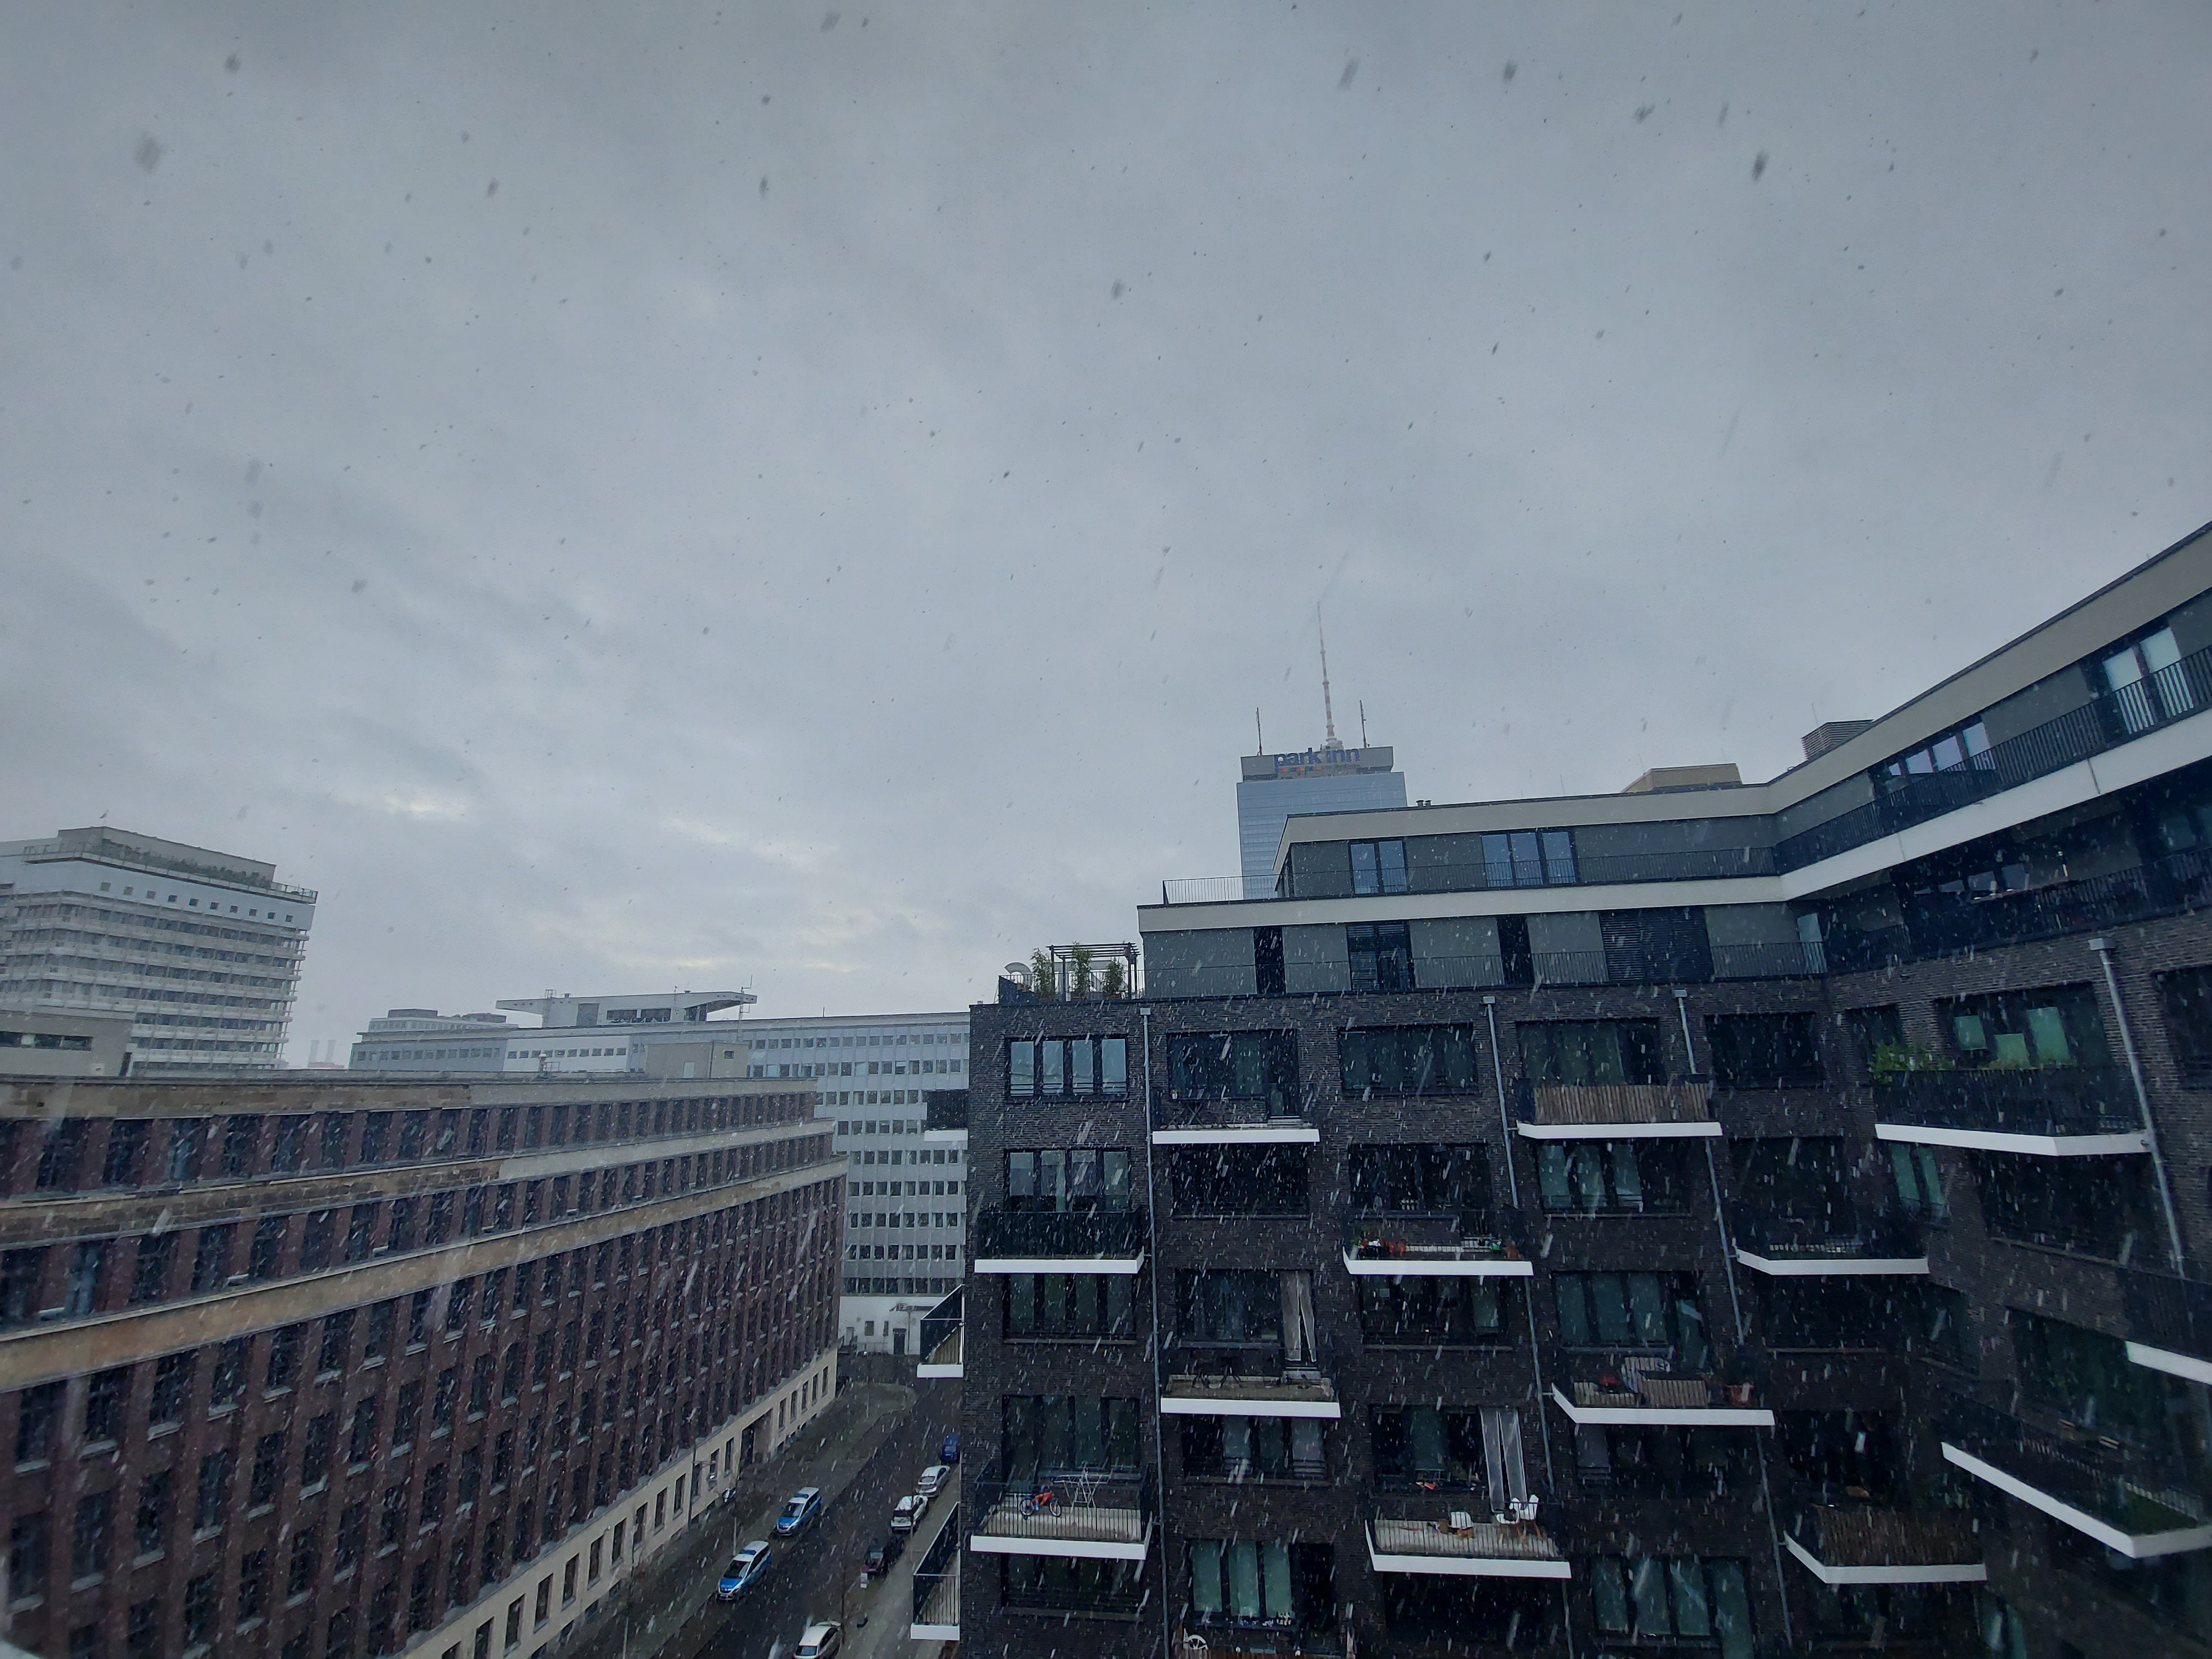
\includegraphics[width = 12cm]{Berlin_winter2020}
	\caption{Winter 2020, Berlin, Germany.}
	\label{fig1}
\end{figure}
Light precipitation (rain $+$ snow) outside the window (see Fig. \ref{fig1})$\ldots$ The room is so quiet that I can even hear my own heartbeat when I lay down: So annoying (see Fig. \ref{fig2})$\ldots$

\begin{figure}[H]
	\centering
	
\includegraphics[width = 12cm]{Arima_Kousei_you_are_in_my_way}
	\caption{Arima Kousei's emotional explosion when performing piano with Nagi, Episode 18: {\it Hearts Come Together}, {\it Your Lie in April} (2014--2015).}
	\label{fig2}
\end{figure}

\begin{quotation}
	``{\it I can't concentrate. I can still hear the sound of the piano. It's in my way. You're in my way, so$\ldots$ Get out of here!}'' - Arima Kousei, {\it Your Lie in April} (2014--2015).
\end{quotation}

I always have this kind of weird feeling\footnote{An indication of bad writing?} when I try to write something \& connect all, or as many as possible, the ideas in my flow of thoughts together, you know? This even does not sound right to me because the question is: {\it How the hell you can organize \& \href{https://en.wikipedia.org/wiki/Connect_the_dots}{connect the dots} when that flow in your head is a real shitty mess?}

In such a situation, as usual, a bad writing habit [no chronological order, switch randomly between English \& Vietnamese\footnote{{\it If the real purpose is to express your thoughts{\tt/}ideas{\tt/}emotions, why does it matter to write under a lot of unnecessary{\tt/}redundant chains{\tt/}constraints{\tt/}criteria?}}, etc.] can be partially accepted \& invoked as an unavoidable replacement to a ``standard'' one: {\it Just let it all out naturally$\ldots$}

Đã mấy tháng nay, mình thường cố ý đi làm trễ khoảng 1 tiếng, để đợi những người khác đến chỗ làm gần đủ hết, vì mình chỉ muốn tránh thủ tục chào hỏi xởi lởi{\tt/}xã giao ``khích lệ tinh thần'' phiền phức mỗi buổi sáng. Mình đánh hơi thấy mùi fake \& bắt đầu trở lên im lặng như một năm về trước. Mình cũng dần dần hiểu được phần nào ý nghĩa của từ ``guồng'' mà các anh lớn hơn với thằng bạn mình hay nhắc tới: Mọi thứ [công việc + cuộc sống cá nhân] bắt đầu lặp đi lặp lại một cách đơn điệu (monotonously), màu sắc cứ dần dần mà phai nhạt ngày qua ngày$\ldots$

À xém chút quên ngữ cảnh, khi những dòng này được viết, mình đã nếm trải 10 tháng đầu tiên của hành trình làm nghiên cứu sinh ở Đức\footnote{Usually called ``PhD'' in general \& ``Doktorand'' in German.} bên Applied Math, cụ thể là về Tối Ưu Hình Dáng\footnote{Dịch thuật ngữ chuyên ngành toán ra tiếng việt thường mang lại cảm giác củ chuối như vậy! Sad$\ldots$} (\href{https://en.wikipedia.org/wiki/Shape_optimization}{Shape Optimization}) cho ống dẫn khí của động cơ đốt trong. Khi mới bắt đầu làm thì mình thấy thích topic này lắm, nhưng đến giữa chừng thì lại bắt đầu chán. {\it Là do mình hay công việc nghiên cứu nó vốn tẻ nhạt như vậy?}$\ldots$

Vào một ngày đông nào đó (vì bữa đó quá đỗi bình thường nên mình chả thèm{\tt/}thể nhớ chính xác là ngày nào) mình lại đạp xe đến chỗ làm, cố gắng tránh né ánh mắt của mọi người. Đến trưa thì đợi ông thầy phụ của mình đi rủ họ ăn chung với nhau, rồi mình lại xách hộp cơm tự nấu đem theo ra khỏi tòa nhà, đến công viên đối diện để ngồi ăn giữa trời tuyết: {\it lủi thủi} \& {\it cô độc}. Vừa ăn trưa mình vừa ngắm chim (ở Berlin chim bồ câu đâu ra cả nùi nùi \& đặc biệt là tụi chim này rất dạng, chắc đất chốn đây hẳn là lành lắm!). Một lát sau mình lại lết lên phòng làm việc. {\it Nặng nề} \& {\it ủ dột}, mình vẫn phải tiếp tục làm những tasks được giao nhưng không hề cảm thấy thích như mọi khi mình được tự ý làm những thứ mình tự chế{\tt/}bày ra nữa. Haizz$\ldots$ Cố làm vậy, rồi từ từ cũng sẽ hết ngày, lại đi về, nấu cơm ăn, xem YouTube đến khi mỏi mắt, rồi ngủ, rồi ngày sau lại lặp lại y như thế: {\it Ôi cái guồng này nó làm mình chán phát điên mất} - mình vừa làm vừa nghĩ vậy$\ldots$

Đợi đến tầm xế chiều, thì cô bạn Maroc ngồi đối diện lưng-lưng (not mặt-mặt) với mình moi ra một hộp Chocolate để tặng mình. Hề cái là cô này phải đợi anh bạn người Đức chung phòng đi lấy{\tt/}nhả nước gì đấy thì cổ mới có dịp để tặng riêng cho mình (phòng mình là phòng toàn PhDs duy nhất của cả nhóm, gồm 3 đứa mình). Tỏ tình? Nah, nhìn lại cái thân hình đang ngày càng trì trệ\footnote{Ironically, I am currently working on Shape Optimization but my body shape gets far \& far away from ``optimal''.} mấy tháng qua của mày đi. Đùa chứ bản nói vì mình đã giúp bản rất nhiều thủ tục giấy tờ - mà mình đã phải vật lộn rất nhiều trong mấy tháng đầu nhờ đợt dịch - khi mới tới nên bản biết hơn (mình đổi từ ``cổ'' sang ``bản'' vì mình để ý tên email riêng của cổ: à, thì ra cô này bằng tuổi mình). Bản nói bản biết ơn mình \& ông thầy phụ của mình lắm, trong mắt cô bạn mới tới thì đây là 2 người tử tế giúp đỡ bản nhiều nhất trong nhóm$\ldots$

{\it Ồ, thì ra vẫn có người trong nhóm xem mình là người tốt{\tt/}tử tế à?} Thật tình thì lúc mình giúp cô bạn thì mình chả nghĩ gì nhiều, giúp thì giúp thôi. Mình là kiểu người ngu dốt kiểu vậy. À không, còn tệ hơn nhiều cơ: {\it a giver}\footnote{\href{https://www.youtube.com/watch?v=YyXRYgjQXX0}{Are you a giver or a taker? | Adam Grant}, TED.}. Việc mình trở thành 1 giver chắc là do ảnh hưởng từ mẹ mình. Hồi nhỏ mẹ mình hay dạy là con cứ tốt với mọi người xung quanh thì họ sẽ tốt lại với con thôi, chứ đừng cứ sống ích kỷ rồi không ai chơi với con hết, đại loại vậy. Đó cũng là bài học đối nhân xử thế đầu tiên của mình \& ảnh hưởng đến tính cách mình rất nhiều$\ldots$

Nghe cô bạn cảm ơn, mình nhìn hộp Chocolate, một chút vui thoáng qua nhưng cũng chợp tắt thật nhanh. Mình không cho phép mình vui lâu hơn vì chắc gì đó là những lời thật lòng, hay {\it chẳng qua chỉ là xã giao với nhau để được giúp nhiều hơn mà thôi?} Vì mình hiểu rằng bất kể mình có tốt bụng \& tử tế cỡ nào đi chăng nữa, cô bạn này sau một thời gian nữa sẽ ghét \& khinh mình vì những lời xuyên tạc từ những người khác trong những bữa ăn trưa tưởng chừng như thân thiện giữa các đồng nghiệp với nhau đó mà thôi$\ldots$

Một lúc sau thì anh bạn Đức về phòng. Anh này hiện đang chí mí cuối năm cuối PhD \& đang bức tốc để chuẩn bị về đích{\tt/}lên đỉnh Olympia, à nhầm, bảo vệ. Mình ngỏ ý chia 50--50 với ảnh, để cho không khí trong phòng 3 đứa mình đỡ căng thẳng. Anh từ chối thẳng, yêu cầu mình để anh ấy yên, anh ta không cần bất cứ thứ gì từ mình. Uầy, vô tình chuốc thêm căng thẳng rồi. Ngu người thật. Đành ăn một mình vậy. Bụng mập càng thêm mập$\ldots$

Cô bạn nói mình lần sau sẽ mua loại ngon hơn, lần này thì chỉ còn loại đó. Có vẻ thật lòng - mình nghĩ. Xem ra mình còn chút hy vọng xót lại vào humanity trong mối quan hệ giữa người với người. Mà nếu cô bạn canh để tặng quà Giáng sinh thì bữa đó là ngày 18 tháng 12, ngày đi làm cuối cùng của năm 2020, giờ mình mới có manh mối để nhớ ra ngày đó. Mùa nghỉ đông đầu tiên kéo dài hơn 40 ngày cuối cùng cũng bắt đầu\ldots

Khoảng thời gian nghỉ đông này rất quý giá để mình đầu tư vào work-life balance lại, bằng cách$\ldots$ làm việc nhiều hơn \& đặc biệt là chỉ làm những thứ mình muốn, chứ không phải những tasks nhàm chán, đôi khi ngu xuẩn, mà ông thầy phụ mình cứ thảy cho suốt mấy tháng qua. Đó là cũng là khoảng thời gian yên tĩnh để mình có thể suy nghĩ về những chuyện đã xảy ra trong những tháng qua. Có vài chuyện mình không tài nào hiểu nổi, đương nhiên vẫn là những câu chuyện muôn thuở về mối quan hệ giữa con người với con người. Mình mà lị: {\it The Trouble Boy}!!$\ldots$ Đại loại là, từ lúc mới đến Berlin tới giờ, bất kể mình giúp đỡ những người khác mỗi khi họ cần, họ đều cư xử toxic ngược lại, thậm chí có anh postDoc còn verbally bully mình. Thế mà mình cứ ảo{\tt/}hoang tưởng là họ hoan nghênh mình tới để làm việc, trao đổi kiến thức \& cống hiến cơ đấy, nhưng thì ra suất Marie--Curie này không dễ ăn{\tt/}handled như mình vẫn tưởng bở. Môi trường học thuật mà thằng ngu này! Mình lại suy nghĩ quá đơn giản rồi. Chán cái đầu nông cạn{\tt/}ngây thơ (naive) của mình thật! Thôi cứ đành ngậm họng lại, tránh tiếp xúc với mọi người (đương nhiên là ngoại trừ boss bự với boss nhỏ, ngu thì ngu chứ chưa muốn bị đuổi!) để khỏi bị bắt nạt, \& giữ năng lượng để tập trung làm việc vậy$\ldots$ Còn 2 năm mấy, 3 năm nữa cơ mà! Đừng có kiểu mới nhập Viện chưa bao lâu mà đã gục{\tt/}tịt ngòi chứ!$\ldots$

Ấy vậy mà, mặc dù đã tập trung làm việc miệt mài, tinh thần \& cảm xúc mình vẫn bị kéo xuống liên tục, \& các mối quan hệ với đồng nghiệp cứ thế càng ngày càng tệ: {\it Thà không có thì tốt biết mấy!} - Mình chợt nghĩ. Cứ thế này thì mình sẽ bị vắt kiệt (drained out{\tt/}\href{https://en.wikipedia.org/wiki/Occupational_burnout}{occupational burnout}) mất. Hóa ra hy vọng, niềm hân hoang, etc. chỉ là những thứ cảm xúc vô nghĩa mình tự tạo ra, để tự huyễn hoặc, \& làm tiền đề cho sự chán chường nặng nề \& thất vọng tột độ mà thôi$\ldots$

Được cái là ông thầy phụ (co-supervisor) của mình rất có tâm. Ổng giúp mình rất nhiều khi mình mới tới Berlin, từ cả nhà cửa, giấy tờ thủ tục, đến hầu hết tất cả các khía cạnh trong công việc. Nhận ra mình đang có dấu hiệu xuống tinh thần, ổng đôn đốc mình làm việc nề nếp, khoa học hơn, giao nhiều tasks hơn, \& rồi cứ 4 giờ chiều mỗi ngày mình sẽ đến tận phòng để gặp \& báo cáo ổng theo mệnh lệnh ở Thư viện chung, trước mặt của các nữ sinh viên đang học Master của nhóm. Thật tình thì đa số mấy tasks ổng giao mấy tháng gần đây có phần ngô nghê \& vớ vẩn thiệt. {\it Hay lúc nào cũng nhảm vậy nhỉ? Hay do mình đã tiến bộ mà không tự nhận thức được?} Không phải chảnh, đơn giản vì mình là người trực tiếp upgrade software, line-by-line, nên mình hiểu rõ nhiều cái technicals mất dạy mà phải tốn có khi cả tháng mới vượt qua được, nên nhiều cái ổng không biết mà chỉ bậy{\tt/}bừa{\tt/}xàm cũng không phải là điều quá ngạc nhiên. Mình là người kiểu vậy: Không quan trọng supervisor khủng (vì họ chỉ tổ bận mà thôi), chỉ cần supervisor có tâm là được. Tình cảm thầy trò vẫn quan trọng hơn là những danh tiếng hào nhoáng (reputation) mà mình chỉ hưởng xoáy chứ không phải có được nhờ chính thực lực của mình.

Tasks ngu thì ngu nhưng kệ vậy, miễn ổng tốt với mình là được rồi, cứ làm nhiệm vụ được giao vậy. Rồi sẽ ổn cả thôi, dù ảm đạm \& cô độc đến cỡ nào đi nữa $\ldots$

Mình chợt nhớ lại 10 tháng trước. {\it Mình làm ở đây mới có 10 tháng thôi mà đã thay đổi nhiều vậy cơ á?} 10 tháng trước, mình lao vào giữa vùng dịch, để làm lại từ đầu lần nữa. Quyết liệt \& dữ dội, tưởng chừng không có gì cản trở được mình nữa, thì mình lại bắt đầu có dấu hiệu gục hệt như một năm trước lúc mình học Master về Pure\footnote{``Pure'', not ``poor''. But, actually, they sound similar. \& that is exactly the reason why I have switched from Pure Math to Applied Math.} Math ở Pháp. Thật tự đáng hổ thẹn \& thất vọng$\ldots$

Khoảng thời gian nghỉ đông tĩnh lặng \& lạnh lẽo giúp mình có thể tập trung suy nghĩ sâu hơn, về nhiều thứ cực kỳ mâu thuẫn đã \& đang diễn ra khiến mình thật sự bối rối \& bắt đầu nghi ngờ. Điều này làm mình chợt nhớ lại cuốn sách \cite{Bancroft_why_he_do,Bancroft_why_he_do_VN} về ``{\it Kẻ thao túng tâm lý{\tt/}bạo hành tinh thần}'', mà mình biết tới nhờ một lần đọc một psychology post về ``{\it Kẻ bạo hành âm thầm}''. Well, thực tình mà nói đây là một cuốn sách về bạo hành gia đình, cả bạo hành thể chất lẫn bạo hành tâm lý nhưng chú trọng đặc biệt về bạo hành tâm lý, cụ thể là tác động từ người chồng gia trưởng lên người vợ lẫn những đứa con đáng thương của ông ta. {\it Daijoubu desu!} Mình vẫn còn con nít mà, nên vẫn có thể áp dụng vế sau lên chính trường hợp của mình được!

{\it Một luồng những suy nghĩ, câu hỏi tự vấn từ sâu trong nội tâm bắt đầu tuôn trào}\footnote{Actually, I have been seriously overthinking about my overthinking problem all the time!$\ldots$ {\it Wait, should I overthink about that also?!!}} $\ldots$

{\it Another flow of thoughts} $\ldots$
\begin{itemize}
	\setlength\itemsep{0em}
	\item {\it Why did almost all of my colleagues treat me so toxic like that despite the fact that I have helped them several times whenever they asked me for my hand. Don't they understand what the term ``grateful'' really means?}
	\item {\it Why does a good person like me have to suffer all these toxic behaviors in lab-environment \& even social isolation?}
	\item {\it Is this world designed for good{\tt/}kind people?}
	\item {\it Does there exist a place on this Earth for all human beings with full of purely good intentions to live \& work?}
	
	In a moment, it seems to me that there is no place for a person with low \href{https://en.wikipedia.org/wiki/Emotional_intelligence}{Emotional Intelligence} (EQ) \& very low \href{https://en.wikipedia.org/wiki/Social_intelligence}{Social Intelligence} (SI) but \href{https://hsperson.com/}{Highly Sensitive} (HSP) like me in this cruel world.    
	\item {\it Why do I have to avoid all these people \& develop psychological problems, especially \href{https://en.wikipedia.org/wiki/Impostor_syndrome}{imposter syndrome}\footnote{The \#1 mental illness in academic{\tt/}lab environment?}?} I have conducted a lot of tasks, even much more than my predecessors, then {\it why do I have to keep suffering?}
	\item {\it Why were I called ``The Lucky Guy''? Why does hardly anybody give a minimum level of respect to me even when I have been conducting such a huge amount of work? Is it because my skin is too yellow to be considered white enough?}
	\item {\it Why do I have to do these stupid{\tt/}bullshit tasks \& report daily to my co-supervisor. \& especially, whenever I refused to do such an unnecessary{\tt/}redundant task, he started to be wildly angry immediately?} But he is a truthfully good, kind, honest, \& enthusiastic co-supervisor, because he has helped me a lot through these tough times in this strange year.
\end{itemize}
I really do not understand: {\it absolutely confused} \& {\it overwhelmed}$\ldots$

{\it Tại sao mình có cảm giác bị đâm lén sau lưng liên tục nhưng không biết chính xác là ai cả? Tại sao ai cũng đối xử mình như thứ rác rưởi mặc dù mình giúp họ khá nhiều? Tại sao mình cảm giác bản thân không đủ tốt \& làm việc chưa đủ cần cù trong khi mình đã làm được những điều mà những người tiền nhiệm ở vị trí của mình chưa từng làm được: ví dụ nâng cấp phần mềm được phát triển \& sử dụng suốt 10 năm trong vòng chưa tới 10 tháng?}

Yeah, everything is so weird, very weird, super weird. This kind of feeling is exactly like there is an invisible ``Black Hole of Truth'' somewhere behind your back. You can feel its existence as a blur, but you cannot see it or touch it directly. So annoying$\ldots$ Very tired$\ldots$ Completely exhausted$\ldots$

- {\it Can you figure out the reason why I hate such a ``Black Hole'' that much?}

- Is it because that hole is black?

- No, you racist fuck! Because$\ldots$ Like the way every matter, e.g. light (`photon') is rapidly sucked towards the `singularity' at the center of a real \href{https://en.wikipedia.org/wiki/Black_hole}{Black Hole}, all truths are also sucked towards this ``Truth Destroyer'' \& then demolished{\tt/}consumed by it.

{\it Có phải mình đang cố đổ lỗi lên mọi người xung quanh để chối bỏ mọi chuyện tệ hại là lỗi của mình không?}

- Không hề.

- Xì{\tt/}hừm{\tt/}hứ{\tt/}etc., thằng nhãi ranh đó lại thế, chả bao giờ biết tự nhận{\tt/}chịu trách nhiệm (take the responsibility), chỉ biết đổ lỗi lên đầu người khác. Xem ra việc làm nghiên cứu sinh tưởng chừng sẽ giúp nó trưởng thành, chín chắn hơn phần nào nhưng giờ nó lại thế, vẫn thế, có khi còn tệ hơn! Đảm bảo nó sẽ mãi là đứa con nít không bao giờ lớn nổi.

- Ừm, có khi nói vậy cũng đúng phần nào$\ldots$

Tới đây thì bạn cần hiểu một điều rằng: {\it khi bạn tự thấu hiểu chính bản thân từ bên trong, thì mọi lời phán xét{\tt/}đàm tiếu bên ngoài không còn quan trọng nữa}$\ldots$

Mình không thể nào nói là mình không quan tâm (I do not care!) tới những lời phán xét như vậy, bởi vì thực sự là mình có quan tâm. Mình quan tâm là vì mình muốn bảo vệ sự thật (lại một hành động ngu xuẩn nữa trong chuỗi dài những hành động ngu xuẩn: scientist wannabe, huh?). \& một trong những bước cốt lõi để bảo vệ sự thật đó là phát hiện những lời giả dối{\tt/}đàm tiếu{\tt/}vu khống (Lie Detector) \& điều chỉnh những lời phát xét bị biến dạng (distorted judgments) do tác dụng của chính cái ``Black Hole of Truth'' gây ra$\ldots$

{\it Bạn biết vì sao nhiều người thích phán xét thế không?} Đó là vì việc phán xét rất dễ: không cần phải suy nghĩ{\tt/}động não nhiều, không cần tốn quá nhiều sức, chỉ cần hướng thẳng tới việc công kích{\tt/}đả thương người khác là bất cứ ngôn từ nào phát ra từ miệng một người tự nhiên{\tt/}tự động{\tt/}mặc định trở thành lời phát xét tiêu cực (đôi khi chết người) ngay lập tức. {\it Thế thì nghe tiêu cực nhỉ? Nhưng nếu bản chất là tiêu cực vậy thì tại sao còn những người muốn làm điều như vậy?} Nhiều là đằng khác! Đó là vì: phán xét tuy rất dễ nhưng đem lại rất nhiều cảm giác sảng khoái cho ``người thẩm phán'': cảm giác tha hồ nếm trải quyền lực{\tt/}sự thống trị  lấn át lên trên nạn nhân để thỏa mãn cái tôi mà không cần tốn nhiều sức lực. Trái lại, việc bình tĩnh suy nghĩ một cách thấu đáo để thực sự hiểu một vấn đề lại khó hơn rất nhiều: đòi hỏi đầu tư nhiều thời gian \& công sức hơn, \& đặc biệt là những kinh nghiệm tích lũy mà thông thường chỉ những người từng trải và{\tt/}hoặc đủ khôn ngoan{\tt/}sáng suốt mới có được. Mặc dù cần đầu tư nhiều như vậy, nhưng điều nực cười là việc thấu cảm (also thấu hiểu, cảm thông) thường không nhận được bất kỳ sự ủng hộ nào từ số đông do ảnh hưởng của tư tưởng bầy đàn{\tt/}hiệu ứng đám đông\footnote{Điều này là đối tượng nghiên cứu chính của nhánh chuyên ngành Tâm lý học đám đông của Tâm lý học xã hội.}. {\it Again, another sad reality}$\ldots$

Uòi uòi uòi, đoạn này hơi bị tâm đắc, dịch lại phát nữa cho bớt sung vại:

{\it Do you know why so many people love judging?} That is because judging is super easy{\tt/}simple: no need to think{\tt/}consider too much \& can be generated effortlessly, the only attempt needed is that you have to concentrate on hurting{\tt/}bullying verbally your victim(s) violently{\tt/}brutally{\tt/}vulnerably, then every single word coming from your mouth will be automatically toxic immediately \& then they form together a deadly judgment. {\it Sound negative, huh? But if the nature of judging is negativity, then why so many people keep doing that?} Although judging is easy, however, in return, it helps them gain a lot of strength \& power: the feeling of tasting the dominance \& several psychological powers over their victim(s) without pending a considerable amount of time \& effort: A {\it hyper-win-lose} situation! On the contrary,
\begin{quotation}
	``{\it In order to be able to think, you have to risk being offensive}.'' - {\sc Jordan B. Peterson}
\end{quotation}
the ability to calm yourself in order to consider{\tt/}contemplate{\tt/}examine events{\tt/}statements{\tt/}situations consciously \& logically\footnote{In reality, the set of non-logical events{\tt/}statements is dense in the set of all events{\tt/}statements, while the set of logical ones, though infinite, has zero measure in that \href{https://en.wikipedia.org/wiki/Universal_set}{universal set}. This pair exists together, both mutually exclusive \& supporting each other simultaneously. Like the way the pair of the rational set $\mathbb{Q}$ \& the irrational one $\mathbb{R}\backslash\mathbb{Q}$ does:
	\begin{itemize}
		\item[(i)] The universal set here is $\mathbb{R}$. The supporting \& mutually exclusive relationships just mentioned can be expressed mathematically by:
		\begin{align*}
			\mathbb{Q}\cup(\mathbb{R}\backslash\mathbb{Q}) = \mathbb{R},\ \mathbb{Q}\cap(\mathbb{R}\backslash\mathbb{Q}) = \emptyset.
		\end{align*}
		\item[(ii)] The set of rationals has Lebesgue measure zero \& their \href{https://en.wikipedia.org/wiki/Cardinality}{cardinality} is the 1st transfinite number, \href{https://en.wikipedia.org/wiki/Aleph_number}{aleph-null} ($\aleph_0$):
		\begin{align*}
			\operatorname{m}_1(\mathbb{Q}) = \operatorname{m}_1(\mathbb{N}) = 0,\ \operatorname{card}(\mathbb{Q}) = \operatorname{card}(\mathbb{N}) = \aleph_0.
		\end{align*}
		\item[(iii)] The cardinality of the set of irrationals is continuum:
		\begin{align*}
			\operatorname{m}_1((\mathbb{R}\backslash\mathbb{Q})\cap[a,b]) = \operatorname{m}_1([a,b]) = b - a,\ \forall a,b\in\mathbb{R}, \mbox{ \& } \operatorname{card}(\mathbb{R}\backslash\mathbb{Q}) = \operatorname{card}(\mathbb{R}) = \mathfrak{c} = 2^{\aleph_0}.
		\end{align*}
\end{itemize}} to connect as many dots as possible, requires much more time \& efforts, especially the expertise{\tt/}experiences, which are usually possessed{\tt/}gained only by hardened and{\tt/}or wise enough individuals. Ironically, in spite of all of these serious investigations, sympathy, empathy, \& humanity have been almost all the time being undervalued{\tt/}underrated{\tt/}underestimated, even ignored from the majority of human beings, which is the prototypical \& fundamental effect of \href{https://dictionary.apa.org/majority-influence}{majority influence}.

\begin{flushright}
	Christmas Eve, Winter 2020. [$-5^\circ$C]--[$-10^\circ$C]. Berlin, Germany.
	
	In the {\it imaginary world} $\mathbb{C}^3$ instead of the {\it real physical world} $\mathbb{R}^3$.
\end{flushright}
Hắn thấy mình đang mệt nhoài, toàn thân rã rời, lê bước trở về phòng riêng trong 1 student studio ở Alexanderflatz\footnote{ {\it Alexander Square}: a large public square \& transport hub in the central Mitte district of Berlin, reputedly the most visited area of Berlin, see \href{https://en.wikipedia.org/wiki/Alexanderplatz}{Wikipedia{\tt/}Alexanderplatz}.}, Berlin--Mitte, sau buổi tối thân mật cùng đồng nghiệp chung team nghiên cứu của hắn. Nói là đồng nghiệp nhưng thật ra không hắn làm việc chung 1 đề tài. Nếu là 1 công việc bên mảng công nghệ hoặc kinh doanh chắc có lẽ sẽ khác. Đây là công việc nghiên cứu. Mỗi người trong team sẽ chịu trách nhiệm 1 mảng nghiên cứu riêng, dù chung 1 research theme, nhưng khó mà làm chung với nhau được. Đấy là cái thất bại đầu tiên của hắn: hắn không tương tác được với đồng nghiệp để tạo ra ý tưởng mới. Nhưng có nên trách hắn không? Hắn chỉ là 1 nghiên cứu sinh bậc tiến sĩ, đồng nghiệp của hắn toàn postdoc -- nghiên cứu sau tiến sĩ, khi mà họ đã rành mảng của họ \& sẵn sàng tương tác với các đồng nghiệp trong nhóm lẫn những đồng nghiệp khác nhóm, thậm chí các giáo sư dạng Head of Research Groups, thì đây là 1 mảng hoàn toàn mới với hắn. Hắn cần thời gian để cày kiến thức nền (background knowledge) -- nhưng đúng ra thì thời gian không cho phép. Hắn đang trong giai đoạn cuối của 1 đề tài sắp nghiệm thu mà các người tiền nhiệm của hắn đã bỏ hẳn. He felt that this project is like a fucking death star which he was still trying to hold on his weak shoulder:
\begin{figure}[H]
	\centering
	
\includegraphics[width = 12cm]{spiral}
	\caption{Rust Cohle's hallucination on The Spiral before the last fight with the Yellow King. \href{https://www.imdb.com/title/tt2356777/}{True Detective} (2014--) [S1.E8: {\it Form \& Void}].}
\end{figure}
Ít ra thì hắn cũng có 1 bài toán nhỏ với thầy của hắn được xuất bản trên 1 tạp chí toán phổ thông nổi tiếng của Đức, tựa tựa tạp chí Toán học \& Tuổi trẻ ở quê nhà của hắn. Hắn mừng lắm. Chẳn phải xuất bản khoa học, nhưng cũng được tính KPI (key performance indicator) để giảm bớt áp lực công việc.

\begin{problem}[Water supply network\footnote{{\sc url}: \url{https://github.com/NQBH/WIAS/blob/master/math_calendar/water_supply_network.pdf}.}, submitted to German {\sc Math Kalendar}, accepted but then rejected]
	Far away in Frozen Kingdom, to guarantee a happy Christmas holiday, Santa Claus \& some elves Alice, Bob, Camille, Dominic, Elsa, Federico, \& Gwen want to set up a water network to supply water to watermills in order to make flour for cookies. Precisely, $m\in\mathbb{N}^\star$ water supply factories denoted by $(F_i)_{i=1}^m$ will supply $n\in\mathbb{N}^\star$ watermills $(W_j)_{j=1}^n$. For each $i = 1,\ldots,m$ \& $j = 1,\ldots,n$, the factory $F_i$ stores water of volume $V_i$ in its own water tank \& is connected to the watermill $W_j$ by an individual empty pipe, denoted by $p_{ij}$ being uniformly cylindrical with the size uniquely characterized by a fixed wall thickness $\delta > 0$, length $l_{ij}$, \& radius $r_{ij}$ of its interior. At the inlet of each pipe $p_{ij}$, a water pump engine is configured to supply water with a constant \emph{volumetric flow rate}\footnote{{\it Volumetric flow rate} of water is defined to be the volume of fluid $V$ which passes during a period of time $t > 0$: $Q\coloneqq\frac{V}{t}$.} $Q_{ij}\ {\rm m}^3${\tt/}{\rm s}.
	\begin{table}[H]
		\centering
		\begin{tabular}{|l|l|}
			\hline
			Notation & Meaning \\
			\hline
			$p_{ij}$ & the uniformly cylindrical straight pipe connecting $F_i$ with $W_j$ \\
			\hline
			$\delta$ & thickness of each pipe in the network \\
			\hline
			$l_{ij}$ & length of the pipe $p_{ij}$ \\
			\hline
			$r_{ij}$ & radius of the interior of pipe $p_{ij}$ \\
			\hline
			$Q_{ij}$ & volumetric flow rate within the pipe $p_{ij}$ \\
			\hline
		\end{tabular}
	\end{table}
	Santa Claus considers the problem that the pipes may get frozen: The longer water flows inside the pipe the more amount of water turns into ice according to the \emph{freezing rule}: ``The water freezes uniformly along the pipe from the wall to the interior \& the thickness of the ice layer is $\tau\alpha$, with $\tau\ge0$ the duration water that has been running through the pipe \& $\alpha > 0$ a constant freezing rate (here we neglect the fact that water arrives at the outlet a bit later than at the inlet). Furthermore, when water freezes, its volume expands by $\approx9\%$.
	
	To prevent pipes from getting broken due to that volume expansion, Santa Clause chooses a fixed small positive number $\varepsilon$ 1st \& requires all the pipes to be designed such that their radii are larger than $\varepsilon$. For each pipe $p_{ij}$, the associated water pump engine will stop pumping if the thickness of the ice layer equals $r_{ij} - \varepsilon$ or the water tank of $F_i$ is empty. When a water pump engine stops, we assume that the remaining water between the ice layer flows immediately to the corresponding watermill, \& we call that pipe \emph{almost frozen}.
	
	Moreover, to build this network of pipes, there is a fixed amount of steel available which can be used to produce at maximum $M_0\ {\rm m}^3$ pipe walls. Santa Claus asks the elves: ``To compute the amount of steel used to build our network, we need to know the total volume of all pipe walls. How can we compute it in terms of the size of the pipes?''
	\item(i) {\sf Amount of necessary steel.} Elf Alice says: ``The total volume of all pipe walls is given by $\delta\sum_{i = 1}^m\sum_{j = 1}^n \pi r_{ij}^2l_{ij}$.''
	
	Santa Claus continues to ask: ``What can be said when there is no pipe getting almost frozen?''
	\item(ii) {\sf Criterion for almost frozen pipes.} Elf Bob says: ``There is no pipe getting almost frozen iff the following inequality holds:
	\begin{equation*}
		\frac{r_{ij} - \varepsilon}{\alpha} > t_i\coloneqq\frac{V_i}{\sum_{j = 1}^n Q_{ij}},\ \forall i = 1,\ldots,m,\,j = 1,\ldots,n.\mbox{''}
	\end{equation*}
	\item(iii) {\sf Total length estimate.} Elf Camille says: ``The \emph{total length} $l\coloneqq\sum_{i = 1}^m\sum_{j = 1}^n l_{ij}$ of all pipes in the network satisfies
	\begin{equation*}
		l < \frac{M_0}{\pi\delta(\delta + 2\varepsilon + 2\alpha\min_{1\le i\le m} t_i)}.\mbox{''}
	\end{equation*}
	\item(iv) {\sf Length estimate.} Elf Dominic says: ``If the total length of all pipes of each factory are equal, i.e., $\sum_{j = 1}^n l_{ij} = l_0$, $\forall i = 1,\ldots,m$ \& a $l_0\in(0,\infty)$, then
	\begin{equation*}
		l_0 < \frac{M_0}{\pi\delta(m\delta + 2m\varepsilon + 2\alpha\sum_{i = 1}^m t_i)}.\mbox{''}
	\end{equation*}
	\item(v) {\sf Capacity estimate.} Elf Elsa says: ``If the total length of all pipes of each factory are equal, the \emph{total capacity} $V$ of all the pipes, defined by
	\begin{equation*}
		\tag{V}
		V\coloneqq\sum_{i = 1}^m\sum_{j = 1}^n \pi r_{ij}^2l_{ij}
	\end{equation*}
	satisfies
	\begin{equation*}
		V > \pi l_0\sum_{i = 1}^m (\varepsilon + \alpha t_i)^2.\mbox{''}
	\end{equation*}
	Santa Claus asks again: ``What can be said if there is no water left in any water tank?''
	\item(vi) {\sf Criterion for empty tanks.} Elf Federico says: ``There is no water left in any want tank iff
	\begin{equation*}
		\sum_{j = 1}^n (r_{ij} - \varepsilon)Q_{ij}\ge\alpha V_i,\ \forall i = 1,\ldots,m.\mbox{''}
	\end{equation*}
	Santa Claus asks: ``In each watermill, bakers will need $10\ {\rm cm}^3$ water to make a cookie. If there is still water in all water tanks after all water pump engines have stopped pumping, how many cookies all watermills can make at maximum?''
	\item(vii) {\sf Amount of cookies.} Elf Gwen says: ``The maximum number of cookies all watermills can produce is given by
	\begin{equation*}
		\sum_{i = 1}^m\sum_{j = 1}^n \left\lfloor10^5\left(Q_{ij}\frac{r_{ij} - \varepsilon}{\alpha} - \frac{\pi}{1.09}r_{ij}^2l_{ij}\right)\right\rfloor.\mbox{''}
	\end{equation*}
	Here $\lfloor x\rfloor$ is the \emph{integral part} of $x\in\mathbb{R}$ which is the largest integer that does not exceed $x$.
	
	Which elves are wrong?
\end{problem}
Actually, no elf is wrong. {\it The only person being wrong is me}.

\begin{quote}
	{\sf Hồng [24; 1st-year Mathematical PhD student]}: Ban đầu thầy tôi bảo đây là 1 tờ báo uy tín về Toán Sơ Cấp (Elementary Mathematics) cho học sinh trung học cơ sở (secondary school) \& trung học phổ thông (high school) của Đức, tương tự như Tạp chí Toán học Tuổi trẻ (abbr., TH\&TT) ở Việt Nam. Tôi nghe mê lắm, nên nhận việc, mặc dù còn nhiều thứ phải làm do tôi đang chuyển từ mảng Giải Tích thuần túy (Mathematical Analysis) sang Toán Tối Ưu (Mathematical Optimization{\tt/}Programming). Thầy tôi bảo cứ làm 1 bài về mạng lưới cung cấp nước (water supply network) với bản chất là quy về việc giải 1 hệ phương trình tuyến tính bình thường (a typical system of linear equations). Như thế thì dễ quá, khó được accept, tôi bảo thầy tôi thế -- đương nhiên bằng tiếng Anh. Nên tôi chế ra bài toán này. Thầy tôi trêu để xem trình độ Toán phổ thông Việt Nam thế nào. Ai ngờ ông ta đã không giải được rồi quê nên quạu đeo. Máu dồn lên mặt đỏ rực, ánh mắt tức bực, sát khí hừng hực. Cuối cùng ông dùng email của ông ta hoặc email của tôi thông báo với Ban Tổ Chức rút bài toán đã được chấp nhận \& sẵn sàng được xuất bản đó.
	
	{\sf Hồng [28; Detective]}: Nhưng sao anh phát hiện được? Đâu có bằng chứng gì?
	
	{\sf Hồng [24; 1st-year Mathematical PhD student]}: Tài khoản GitHub của tôi là bí mật, vì thậm chí tôi còn chả nhớ là đã hứng lên tạo nó vào lúc mới mua laptop đầu năm 2 Đại học. Tôi dùng nó điền bừa vào CV. Nên chỉ có ai có CV của tôi thì mới biết được tài khoản GitHub của tôi. Tức chỉ có tôi \& thầy tôi. Vào đúng ngày Ban Tổ Chức công bố bài, tôi vào Traffic của trang GitHub thì thấy có 1 người khác vào. \& Ban Tổ Chức đã quyết định xóa bài của tôi vì vi phạm yêu cầu là đã có lời giải trên mạng trước. \& chẳng có lời giải nào cả: tôi đơn giản là chỉ để cái đề (problem) lên đấy, không có bất cứ solution nào kèm theo. Tôi cũng chả cho ai biết tài khoản của tôi với cái link ngoằn ngoèo khó kiếm kiểu đó cả. Phải cay cú, hận thù lắm thì mới lục tung cả lên để quyết tìm ra cái link như thế. {\it Mà tôi có làm gì sai chứ?} Tôi chỉ nhất thời chế bừa ra 1 bài toán sơ cấp về tối ưu hóa hệ thống cung cấp nước dành cho học sinh Trung học Phổ thông mà thầy hướng dẫn luận án Tiến sĩ Toán Tối Ưu người Đức của tôi không thể giải ngay được. Chỉ có vậy.
\end{quote}
Sáng Giáng sinh năm ấy hắn dậy sớm, ra siêu thị mua đồ ăn ngon. Lâu lâu tự  biết thưởng cho mình 1 bữa ngon lành thay vì cứ mua đồ giảm giá để tiết kiệm tiền gửi về nhà \& để dành sau này lập gia đình, nuôi con hắn 1 cách chu đáo, cố rút kinh nghiệm từ cha hắn \& cha của cha hắn. 

There have been many broken pieces of memories in his head. Good memories. Bad memories.

Hắn nhớ lại cha hắn. Chợt hiểu ra vài thứ. Có lẽ hắn không có khả năng để tạo hạnh phúc cho người khác. Nếu có khả năng về mặt thuần tình cảm thì cũng chả có vị thế về vật chất. Hắn chấp nhận rồi buông bỏ.

\begin{quote}
	{\sf ? [24]}: {\it Sao mày có thể nghĩ tới chuyện thầy hướng dẫn người Đức đang đố kỵ với mày hả cái thằng ngu dốt đần độn kia?} Người Đức nổi tiếng trung thực, thẳng thắn, tôn trọng công việc hơn mạng sống mà? Thậm chí ông ta trước khi làm Research Scientist, tức cánh tay phải của ông Giám đốc như hiện tại, thì cũng là Junior Professor của Đại học Humboldt đấy? Tích góp kiến thức toán học chừng đó năm mà mày lại nghĩ là ổng đố kỵ nên ngấm ngầm hại mày à? Mày nói ra mà chẳng biết ngượng miệng sao?
	
	{\sf Hồng [24; physicist wannabe]}: Việc tích góp kiến thức nhiều năm cũng na ná việc độ dịch chuyển của 1 người có lợi thế xuất phát sớm thì đương nhiên sẽ bỏ xa 1 kẻ trẻ người non dạ mới đặt chân vô vạch xuất phát \& chổng mông lên chuẩn bị chạy vậy. Nhưng vấn đề ở đây không phải là độ dịch chuyển $\vec{\bf d}$ hay tọa độ ${\bf x}$ trên cuộc đua kiến thức, e.g., về Toán học như anh nói, vấn đề ở đây là vận tốc ${\bf v} = d{\bf x}{\tt/}dt$, à không, tôi xin lỗi, cái quan trọng ở đây là ông thầy của tôi nhìn thấy cái gia tốc ${\bf a} = d{\bf v}{\tt/}dt = d^2{\bf x}{\tt/}dt^2$ đến khác người của tôi. Tôi đã làm việc đến đêm muộn \& không biết ngày nghỉ là gì. Thậm chí vận tốc của gia tốc đó $d^3{\bf x}{\tt/}dt^3$ hoặc gia tốc của gia tốc đó $d^4{\bf x}{\tt/}dt^4$. Anh có hiểu không? Mỗi lần tôi tính ra 1 kết quả hoàn toàn mới, như cái adjoint equation siêu phức tạp của $k$-$\epsilon$ turbulence model mà trước đó chả có ai dám tính tay cả nói chi tính không nổi. Thầy của tôi tỏ ra khó chịu cực kỳ \& kiểm soát vi mô (micro-manage) tôi ngày nhiều hơn. Thậm chí tôi có làm hết \& thầy tôi chỉ hướng dẫn, đưa ra vài mệnh lệnh \& đứng tên chung thì ông ta vẫn khó chịu. Vấn đề không phải là tôi gồng mình làm hết \& ông ta có thể ở không hưởng thụ. Vấn đề là ông ta chả muốn tôi có bất cứ sản phẩm khoa học nào cả \& ông ta quyết tâm phá. Chỉnh vài công thức thành sai hoặc đổi style gõ. Tôi bị chứng rối loạn ám ảnh cưỡng chế (Obsessive--Compulsive Disorder, abbr., OCD) nữa. Tôi không thích điều đó nhưng vẫn im lặng sửa cho đúng vì tôi là học trò, là cấp dưới. Sửa sai không đủ đô nên ông ta tiếp tục xóa vài thư mục lúc tôi đi ăn vì 1 lần sơ suất không chú ý nên bị ông ta phát hiện mật khẩu khi đứng đằng sau lưng tôi mà tôi không hay. Nếu trong não tôi có 1 cái giếng hay 1 mạch nước ngầm mà tất cả sự sáng tạo của tôi từ đó chảy ra, thì ông ta sẽ lấp nó, phá hủy nó. 1 sự tiệt diệt của cội nguồn sáng tạo: ông ta muốn bứng cái gốc sáng tạo của tôi ra, phá hoại đến chừng nào nó không còn sản xuất ra được bất cứ cái gì mang tính sáng tạo nữa thì thôi: He is a {\it Creativity Destroyer}. \& he knows how to do it properly \& even creatively. He is excellent at that shit instead of solving a high school mathematics problem proposed by his own PhD student. I am his 1st PhD student.
\end{quote}
Thế ông ta làm kiểu quái nào mà có thể hủy diệt cái mạch nước ngầm của sự sáng tạo trong não 1 thanh niên sung sức 23--24 tuổi? Chúng tôi sẽ bàn kỹ về điều này hơn ở Sect. \ref{sect: psychological manipulation}: {\it Psychological Manipulation}.

A dark student room in Alex-Wedding-Strasse, opposite the main Police station. No sound. No sign of life. He can't feel anything from himself. He is not presented.

Hắn chợt choàng tỉnh dậy sau cơn mê man, đầu óc mụ mị, nhức như búa bổ. Mình phải tính tay cho xong -- hắn nấu 1 ít rồi ngồi vào bàn \& làm việc. Hắn không muốn những cảm xúc. Hắn cho những thứ đó là cấm kỵ của 1 người làm khoa học. Quá ủy mị. Quá mềm yếu. Hắn cứ lờ đi mặc dù tiềm thức cảnh báo hắn.

\begin{quote}
	God. It's just a fucking simple work. Just get it done. Move to something else.
\end{quote}
Hắn ước gì phiên bản tương lai của hắn sẽ quay trở về giúp hắn, cho hắn 1 lời khuyên hay ho nào đấy hoặc đấm 1 cú trời giáng thẳng vào bộ não ngây thơ của hắn để hắn tỉnh ngộ, thậm chí thức tỉnh. Chả có ai giúp hắn cả. A contradiction in both his drinks \& his subconscious mind. He works in mathematics so long to avoid contradiction, now it comes to his lifestyle, his psyche. Fucking ironic.

Hắn say xưa làm việc. Phòng bên hì hục làm tình. Sự thăng hoa hắn tự cho là đã tìm thấy trong công việc \& sự khoái cảm của bộ trai gái phòng bên hòa hợp, át đi tiếng siren còi hú inh ỏi của đồn cảnh sát. Nhịp nhàng. Giống như vũ điệu reo hò soran, 1 nét văn hóa đẹp của người Nhật. Hắn thấy (chị) Trinh, 1 junior software developer tại Amazon, nhắn. Chắc lại nhờ vả gì đó, chị ta chỉ có thế, chỉ xuất hiện khi cần cái gì đó hoặc tỏ ra hơn cái gì đó rồi tốc biến không báo trước -- hắn thoáng nghĩ. Hắn chưa bao giờ hiểu tại sao bạn bè hắn lại cảnh báo chị ta nhiều đến thế. Hắn theo chủ nghĩa ôn hòa, nên dẫu có bao nhiêu red flags hắn vẫn mặc kệ. Nhưng ai ai cũng bảo nên cẩn thận với chị ta. Hắn nhớ lại trước đây, lúc còn năm 2 Đại học, ở Ký Túc Xá Đại Học Quốc Gia ở Thủ Đức, bạn chung phòng của hắn cũng cảnh báo hắn về 1 đứa chung lớp hắn như thế.

He knock a drink of beer. He didn't like wines. Then he drank a lot of black coffee, the pure type. He always has a very bad eating \& drinking habit.

Beer so he can forget bad shits, coffee so he can focus on the good. Actually a side effect of coffee helps him shit well too. The cure for all the sittings long hours labor work.

Thay vì chịu sự cô đơn, hắn thỏa hiệp với vài con người thuần lợi dụng. 

{\it What is missing? What pieces of the big picture of life do I miss? A little self-esteem? A little understanding about how this real life actually works?}

Eo ơi cái di chúc chết tiệt.

Hắn tự huyền hoặc bản thân với 1 trí nhớ tốt như 1 cỗ máy điện tử, sự ảo tưởng sức mạnh về món quà mà hắn được ban tặng.

Nah, these things so difficult. I get back to my mathematics, my calculus.

\subsection{Why bad things always happen to good people? -- Tại sao người tốt luôn gặp chuyện xấu?}
\textbf{\textsf{Resources -- Tài nguyên.}}
\begin{itemize}
	\item \cite{Kushner_bad_things_good_people}. {\sc Harold S. Kushner}. {\it When Bad Things Happen to Good People}.
\end{itemize}

{\it What is the point of all of this?}

Oh oh, so if I can do all these math, my father's liver cancer will disappear right? He can live right? He can be normal again like nothing happens right?

Fucking bullshit. All of this. Purely fucking bullshit.

Hắn tự hỏi liệu Chí Phèo đã cảm giác thế nào vào cái lúc hắn vừa đi vừa chửi. Cái làng Vũ Đại ngày ấy. Vãi đạn thật.


Then he felt awake. Or more precisely, something inside him awoke. He was not sure about it but totally aware of its presence.

This is a very different battle - the one I can't win now. {\it If you lost a battle within yourself, i.e., inner war(s) in your head, then how the hell you can win any other outer battle?}

He had worked so hard to be able to take all the responsibilities of the only job offered to him, then he got judged to be lazy \& irresponsible in many senses.



This is exactly the definition of a kind of battle which he will lose no matter how.

{\it Do I want to die as a good man? Like my father?} No, I want to die as a wise man. 1st, I need to confront my stupidities.

The man who lost his faith in God finds a way to get insight. The journey of revelation begins.

Oppenheimer Homocunlus

You mean Newton is the fuck boy of science? Yo, no! The player. Like Mozart - the player of musical instruments. Here I mean the player of formulas \& concepts.

My conscious mind has still been working with this idea no matter how I deny \& destroy all pieces of my writings. The day my teacher die, the day I remember my father die. Consonant echoes from the past into the present. 

It is about the passion.

Power of concentration -- black fist in JJK.

\begin{center}\it
	Feeds the dying light, \& brings me back to life\\
	Let the darkness lead us into the light 
	-- Ignite, {\sc Alan Walker}
\end{center}
Then the most dangerous intrusive thought won:

Hay là mình tạm ngưng làm toán mà thử làm nhà văn nhỉ? -- You're fucking kidding me right? Don't fool yourself. Joke on all of us.

Winter that year so cold, colder than before. He felt the damn cold in his own mind \& own heart.

He has no literary gift, not a single gift for conceptual thoughts, just some average mathematical computation skills, not abstract enough to become a Pure Mathematician, not complex or useful enough to become an Applied Mathematician. {\it Who the hell can he become then?}

But the day his son, if he has any, asks him about these, {\it what kind of father is he then?}

I don't know what the fuck do you want. I really have no idea. \& I am so fucking tired to be pretentious. Listen. Pick your pieces up.

Solitude is inevitable.

Đắm mình trong đại dương trầm cảm đủ lâu, hắn cảm thấy 1 sự tự do \& thanh thoát tột cùng, như kiểu đả thông kinh mạch trong \href{https://www.imdb.com/title/tt0373074/}{\it Kung Fu Hustle} (2004) với tựa Việt {\it Tuyệt Đỉnh Kungfu}, nhưng ở đây là đã thông thế giới quan \& nền tảng giá trị của hắn. Nhìn mọi thứ rõ thế này thích thật.

Khi bạn rời khỏi 1 địa hạt nào đó, những người sùng bái, những tín đồ của địa hạt, tôn giáo đó có thể coi bạn như kẻ bại trận (loser), đồ súc vật (animal), thứ rác rưởi (trash), quân phản trắc (traitor), etc., để có lý do tự cho mình cái quyền chà đạp lên bạn. Chả sao cả. Bạn không còn lãnh trách nhiệm mình là 1 mắc xích trong cái luồng công việc ở địa hạt đó nữa. Bạn dành nhiều thời gian hơn cho bản thân, để phát triển bản thân, tự do làm những điều mình thích, bên cạnh việc kiếm tiền trong trường hợp việc kiếm tiền không dính dáng đến sở thích hiện tại của bạn. This is the kind of the ultimate freedom mentioned in \href{https://www.imdb.com/title/tt0137523}{\it Fight Club} (1999).
\begin{quote}\it
	``\& then $\ldots$ something happened. I let go. Lost in oblivion. Dark \& silent \& complete. I found freedom. Losing all hope was freedom.'' -- \href{https://www.imdb.com/title/tt0137523}{\it Fight Club} (1999)
\end{quote}
Naturally \& inevitably, in the autumn of 2021, after the death of his mathematics teacher in high school, in another dark room in The Student Hotel in Vienna, Austria, he decided to fight his primal fears, in the realms of literary -- word \& emotion analysis, \& psychology -- behavior \& emotion analysis, with the help \& guidance of philosophy -- value \& meaning analysis -- so that he can be lost in his flow(s?) of thoughts less frequently, or at least being lost in a positive way this time.

Maybe he never nails it, the kind of thoughts \& writings he always wants to pursue. {\it Is it important though?} Just another lose. He is used to it since he is a loser. But it is still a good try, a way to live aesthetically, spiritually, which means to be able to live properly -- he supposed \& still believes: an initialization of the vague structure of his broken system of beliefs.

\begin{quotation}\it
	``In this world, is the destiny of mankind controlled by some transcendental entity or law? Is it like the hand of God hovering above? At least it is true that man has no control, even over his own will. Man takes up the sword in order to shield the small wound in his heart sustained in a far-off time beyond remembrance. Man wields the sword so that he may die smiling in some far-off time beyond perception.'' -- {\sc Kentaro Miura}, {\it Berserk}, Vol. 1
\end{quotation}
{\sf Tạm dịch}: Trên thế giới này, vận mệnh của loài người có phải do 1 thực thể hay quy luật siêu việt nào đó điều khiển không? Có giống như bàn tay của Chúa đang lơ lửng trên cao không? Ít nhất thì đúng là con người không thể kiểm soát được, ngay cả ý chí của chính mình. Con người cầm kiếm để che chắn vết thương nhỏ trong lòng mình đã phải chịu đựng từ 1 thời gian xa xôi không thể nào quên được. Con người sử dụng thanh kiếm để có thể chết với 1 nụ cười ở 1 thời điểm xa xôi nào đó ngoài tầm nhận thức.

\begin{figure}[H]
	\centering
	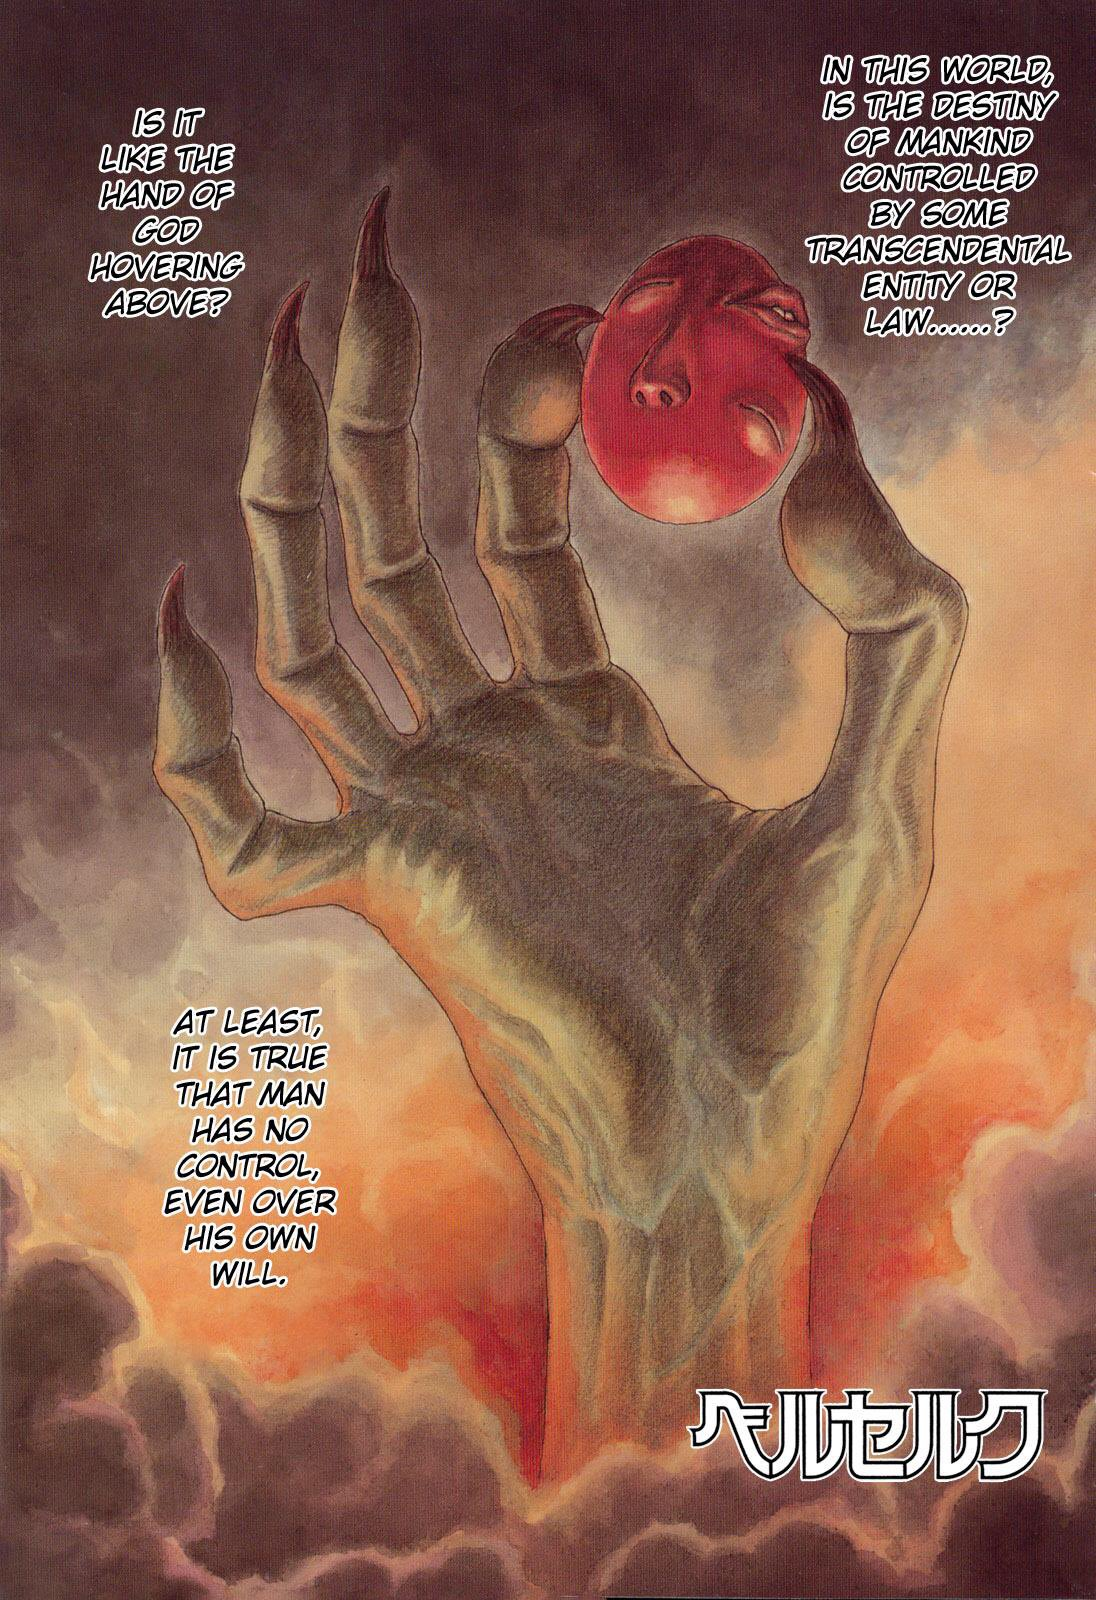
\includegraphics[width = 8cm]{Berserk_behelit_color}
	\caption{The Hand of God holds the Behelit in Berserk.}
\end{figure}

\begin{quotation}\it
	``Providence may guide a man to meet 1 specific person, even if such guidance eventually leads him to darkness. Man simply cannot forsake the beauty of his own chosen path. When will man learn a way to control his soul?'' – {\sc Kentaro Miura}, {\it Berserk}
\end{quotation}
{\sf Tạm dịch}: Mệnh trời có thể chỉ đường 1 người gặp 1 người cụ thể, ngay cả khi sự hướng dẫn đó cuối cùng lại dẫn kẻ đó vào bóng tối. Kẻ đó đơn giản là không thể từ bỏ vẻ đẹp của con đường mình đã chọn. Khi nào con người sẽ học được cách kiểm soát linh hồn của chính mình?
	
\begin{quote}
	{\sf Hồng [?--?; humble philosopher ready to die]}: {\it Do you know what is one of the biggest regrets in life?}
	
	-- Cậu có biết 1 trong những điều đáng tiếc nuối nhất trên đời này là gì không?
	
	{\sf Hồng [23--25; depressed Pure Mathematician wannabe]}: I have no idea. {\it How the hell can I know it?} There are too many regrets in this fucking life in all aspects. What is it according to you?
	
	-- Tôi không biết. Thế đéo nào mà tôi biết được cơ chứ. Có quá nhiều điều để đáng tiếc trong cái cuộc sống chó chết này theo nhiều phương diện. Thế theo ông là cái quái gì?
	
	{\sf Hồng [?--?; humble philosopher ready to die]}: A gifted, talented, or even multi-talented (wo)man without any piece of art, with no contribution \& no legacy for the next generation(s) after him{\tt/}her. What a terrible \& accursed waste of talents \& giftedness!
	
	-- 1 gã{\tt/}ả có tài, thậm chí có nhiều tài hay nhiều loại năng khiếu, nhưng lại không chịu{\tt/}không thể (?) để lại bất cứ tác phẩm nghệ thuật nào, không có 1 chút cống hiến hay truyền lại bất cứ di sản nào cho (các) thế hệ tiếp theo sau hắn{\tt/}ả. 1 sự phí phạm tài năng đến mức kinh khủng \& đáng bị nguyền rủa!
\end{quote}

\section{An Initial Configuration-- 1 Màn{\tt/}Thiết Lập Ban Đầu}
Bằng cách đặt ra 1 số nguyên lý (principles) \& quy tắc (rules), chúng tôi tin là `cuộc thập tự chinh' này sẽ có chỗ để bám níu vào, chúng có tác dụng như những cái mỏ neo, ít nhất để không bị lạc giữa đại dương tri thức mênh mông với những con quái vật của sự vô tri (ignorance monsters) \& những con quỷ của sự ngu dốt \& ác độc (devils of stupidities \& cruelties) chầu chực chờ sẵn dưới đáy đại dương sâu thẳm -- the deep bottom of a dark ocean -- có thể vồ túm lấy ta bất cứ lúc nào khi mà nhận thức của ta bị đánh lừa \& rơi vào trạng thái u mê mất cảnh giác.

\subsection{Rules -- Các quy tắc}
Mỗi người $P$ (abbr., person) có một xuất phát điểm $\{P(t)\}_{0\le t\le t_0}$ khác nhau, được hưởng hoặc bị ép nhồi các nền tảng giáo dục khác nhau, sự tương tác với những người khác nhau, cùng vô vàn những chuyện \& những biến cố họ gặp trong suốt 1 cuộc đời hoàn toàn khác nhau, thành ra nền tảng nhận thức \& xu hướng phát triển nhận thức, cùng sự hình thành các cấu trúc niềm tin \& các hệ giá trị cơ bản cùng thế giới quan của mỗi người hoàn toàn khác nhau.

Quy tắc đầu tiên ở đây là:
\begin{Rule}[On judgment -- Bàn về phán xét]
	Không phán xét, công kích, e.g., dí trên mạng xã hội, bất cứ ai. Cũng không áp đặt ai, thậm chí cả việc áp đặt ai đó không được áp đặt người khác. Tạo cho người khác 1 cảm giác thoải mái tối thiểu khi tiếp xúc.
\end{Rule}

\begin{Rule}[On stalking -- Bàn về rình rập]
	Không quá tò mò vào cuộc sống cá nhân của người khác, e.g., stalk in social media -- rình mò trên các nền tảng mạng xã hội, xâm phạm tài khoản  riêng tư cá nhân bất hợp pháp. Keep healthy boundaries for both.
\end{Rule}

\begin{Rule}[On system reset -- Bàn về khởi động lại hệ thống]
	Một phản tư xa hơn trong tương lai có lẽ là chẳng có hành trình phát triển tự thân nào mà đủ sức chống chọi 1 cách hiệu quả với các tương tác xã hội cả, đặc biệt là các tương tác xấu \& các mối quan hệ độc hại (toxic relationships) cả. Khi đó thì tất cả các ghi chú ở đây sẽ bị xóa. Mọi thứ trở về cấu hình sống nhiều mặt phổ dụng để che giấu bản thân.
\end{Rule} 

\subsection{Goals -- Các mục tiêu}
This writing activity is one of many ways, which is likely to become the main one, to balance between my scientific work \& personal life. I believe some arts will be the tool.

Việc viết lách, theo mình nghĩ, bằng cách này hay cách khác, một lúc nào đó \& theo 1 cách tự nhiên nào đó, cũng sẽ tìm tới những kẻ thích suy nghĩ, những kẻ hay nghĩ nhiều, \& những kẻ mệt mỏi vì cái tật đó, e.g., nhà nghiên cứu, nghiên cứu sinh, các học giả, nói chung là những người làm trong mảng học thuật hoặc phải tiếp xúc nhiều với chữ. Tật hay tài thì chưa biết nhưng ắt hẳn việc viết dùng để sắp xếp mọi thứ trong đầu cho ngăn nắp thì không thể tránh khỏi đối với những người làm việc đầu óc nhiều.

\subsection{Styles -- Các phong cách}

\begin{itemize}
	\item {\it Original style}: khi bắt đầu tự học về nghề viết, chúng tôi tham khảo quyển {\it The Elements of Style} \cite{Strunk_element_style,Strunk_White_element_style} của giáo sư tiếng Anh người Mỹ {\sc William Strunk Jr.} tại Đại học Cornell.
	\item {\it Flexibility like Water}: Tiểu thuyết này không bị ràng buộc bởi duy nhất 1 phong cách viết nào cả. Nếu có đi chăng nữa thì có lẽ đó là {\it phong cách viết tự do -- free style writing}. Đôi khi các bạn sẽ bắt gặp 1 vài đoạn phong cách viết bình dân, đôi khi có những từ ngữ chửi thề tục tĩu kiểu chợ búa như phong cách viết văn của huyền thoại đấm bốc {\sc Mike Tyson} trong quyển {\it Undisputed Truth} \cite{Tyson_Sloman2013}, đôi khi cũng có những đoạn khá hàn lâm học thuật khi bàn về các khái niệm trừu tượng về Khoa học Tự nhiên, hoặc về Tâm lý học \& Triết học. Dáng dấp như vũ điệu twerk của ca sĩ \& nhạc sĩ người Nam Phi {\sc Tyla Laura Seethal} với mệnh danh ``Nữ hoàng nhạc Popiano'' trong bài {\it Water} gây bão trên các bảng xếp hạng âm nhạc 1 thời.
	\begin{quote}
		{\it``Be water, my friend.''} -- {\sc Bruce Lee}
	\end{quote}	
	\item Do kiến thức nền tảng chính của các tác giả là Toán học, nên 1 phần lớn các đoạn văn sẽ được viết với phong cách ngắn gọn, súc tích, các đoạn hội thoại được viết với phong cách kiệm lời, dùng vài từ để diễn đạt như thần giao cách cảm (telepathic style) giữa những người cùng ngành hoặc cận ngành. Bên cạnh đó, với khát vọng chinh phục địa hạt của văn chương, do 2 tác giả đều là những kẻ dốt văn, nên nhiều đoạn sẽ viết dài ra hơn, với hy vọng không lan man \& lạc đề, để phục vụ điều này.
	\item Với mỗi phần (section, subsection, subsubsection), chúng tôi sẽ liệt kê phần {\it Resources -- Tài nguyên} gồm các nguồn tham khảo chính, đa số là sách, bài báo (điện tử), ấn phẩm khoa học, etc., cho phần đó. Mỗi cuốn sách sẽ được trích dẫn kỹ càng để bạn đọc có thể tìm thông tin của chúng ở phần {\it References -- Tài nguyên{\tt/}Tài liệu tham khảo} \ref{ref}. Để kích thích vị giác của độc giả trong việc đọc sách, chúng tôi sẽ kèm ngay theo sau mỗi quyển là 1 thông tin giới thiệu ngắn, đa số lấy từ trang web thương mại điện tử \url{https://www.amazon.com} của công ty công nghệ đa quốc gia của Mỹ {\sf Amazon.com, Inc.} của nhà sáng lập người Mỹ {\sc Jeff Bezos}, cùng vài trích dẫn hay trong sách đó (có thể là highlighted quotes from the book từ chính trang web Amazon hoặc (các) trích dẫn yêu thích trong quyển sách tương ứng của chúng tôi).
	\item I have not read yet, \& unintended to, all the heavy references mentioned in this section, but they seem necessary to be included for the sake of completeness.
	
	-- Tôi đọc, \& cũng không định đọc, tất cả các tài liệu tham khảo được đề cập trong 1 phần nào đó, đơn giản tôi chỉ muốn đọc ``vừa đủ'' để khớp với cảm nhận, nhưng có vẻ khá cần thiết để liệt kê các tài liệu tham khảo đó nhằm đạt được sự hoàn chỉnh.
	\item Each section, subsection needs initiating with {\sf Keywords -- Từ Khóa, Resources -- Tài Nguyên, Goals -- Các Mục Tiêu}.
	
	-- Mỗi phần, phần con sẽ được khởi tạo với {\sf Keywords -- Từ Khóa, Resources -- Tài Nguyên, Goals -- Các Mục Tiêu}.
\end{itemize}

\section{On Writing: Literary writing for a literary retard -- Bàn về việc viết: Học viết văn cho kẻ dốt đặc văn}
\textbf{\textsf{Keywords -- Từ khóa.}} {\it Literary -- văn chương, prose -- văn xuôi, writing style -- văn phong}.

Trước hết, để tôi giải thích cho bạn vì sao tôi là 1 trong những người phù hợp nhất trên cái hành tinh này để viết 1 cái phần có tên là {\it On Writing: Literary writing for a literary retard -- Bàn về việc viết: Học viết văn cho kẻ dốt đặc văn}. Đơn giản vì: tôi là 1 kẻ thiểu năng văn chương đúng nghĩa đen.

\begin{quote}
	{\sf Hồng [4--23.5; typical theoretical agreeable giver]}: But you have to be useful to other people right? You have to write something nice, something educated, something makes people happy, even in a fake way. Whether you are happy when writing or not does not matter.
	
	{\sf Hồng [26--?; critically practical disagreeable writer]}: Fuck off. I write because I like to write, because I need to write to be able to understand myself, \& because I will be good at writing no matter how. I write for myself 1st. Only if I find it useful for other people, I will share to the class of people who need it. You fucking slave! Go fuck yourself.
	
	{\sf Hồng [4--23.5; typical theoretical agreeable giver]}: But you have to be useful to other people \& forget yourself. You have to sacrifice yourself when needed. Only in that way, you can live properly as a good person.
	
	{\sf Hồng [26--?; critically practical disagreeable writer]}: I don't give a single fuck \cite{Manson_giving_fuck,Manson_giving_fuck_vn}. Fucking Jesus Christ!
	
	{\sf Hồng [4--23.5; typical theoretical agreeable giver]}: Hey man. Let me put this matter like this: I know he has been being fixed in the Cross. So he cannot do anything to react or response to your physical action. But please for the mercy of God, don't $\ldots$ Do not do it you $\ldots$ filthy animal.
	
	{\sf Hồng [26--?; critically practical disagreeable writer]}: Oh my fucking gosh! It is true that I am an atheist but what in the bloody hell are you even thinking about my sexuality? Let me alone. Get the fuck out of my head. I need to write.
\end{quote}

\subsection{I want to be a writer -- Tôi muốn trở thành 1 nhà văn}
\label{sect: writer wannabe}
Tên phần này bắt chước tựa đề của quyển {\it I want to be a mathematician: An Automathography} \cite{Halmos1985,Halmos1985_3_parts} (tạm dịch: {\it Tôi muốn trở thành 1 nhà toán học: tự truyện cho nghề làm toán}) của nhà toán học \& nhà triển lãm nghệ thuật về khoa học nổi tiếng người Áo--Hungary {\sc Paul Halmos}.

\begin{goal}
	Transform a writer wannabe into writer.
\end{goal}

\begin{quote}
	{\sf Hồng [25; writer wannabe, literary retard]}: Tôi muốn học viết, anh có cách nào hay sách nào chỉ tôi với.
	
	{\sf Hồng [28--?; writer]}: Nếu anh mới bắt đầu thì tôi nghĩ anh nên đọc quyển {\it The Elements of Style} \cite{Strunk_element_style} (tạm dịch: {\it Các yếu tố của phong cách}) của tác giả người Mỹ {\sc William Strunk Jr.} hoặc bản tái bản có bổ sung \cite{Strunk_White_element_style} của ổng \& đệ tử {\sc E. B. White} để hiểu tầm quan trọng của phong cách viết chuẩn mực, ngắn gọn, súc tích.
	
	{\sf Hồng [25; writer wannabe, literary retard]}: Sau đó thì đến quyển nào? Tại tôi thấy quyển này khá ngắn, \& tôi có thể đọc khá nhanh. Nên tôi nghĩ tôi cần nhiều hơn trong lần `bàn giao tri thức' đầu tiên này. Tôi đoán thế.
	
	{\sf Hồng [28--?; writer]}: Đồng ý là quyển {\it The Elements of Style} khá ngắn, nhưng cần thời gian để cảm thụ các quy tắc. Quyển đấy nhỏ mà có võ. Anh sẽ hiểu ý của tôi sớm thôi khi bắt tay vào viết 1 thứ gì đó của riêng anh.
	
	{\sf Hồng [25; writer wannabe, literary retard]}: Anh thông cảm. Tôi hơi tham vọng về mặt tri thức. Anh có thể gọi là tham lam cũng được. Ambitious \& intellectually greedy. {\it What's so different though?} Anh có thể cho tôi thêm tên vài quyển nữa được không. Phòng trường hợp tôi đọc quyển đầu nhanh quá nên xong, hoặc chán hay khó quá nên (tạm) ngưng.
	
	{\sf Hồng [28--?; writer]}: Chiều ý anh luôn. Tiếp theo là quyển {\it On Writing: A Memoir of the Craft} \cite{King2000,King2010} của nhà văn nổi tiếng về truyện kinh dị người Mỹ {\sc Stephen King}, quyển {\it On Writing Well: The Classic Guide to Writing Nonfiction} \cite{Zinsser2001,Zinsser2016} của {\sc William Zinsser}, đệ tử của {\sc E. B. White}, mà {\sc E. B. White} lại là đệ tử của {\sc William Strunk Jr.}, nên đây là bộ 3 sư phụ--đồ đệ của 3 thế hệ liên tiếp. Sẵn tiện nếu anh muốn viết về quá khứ, kiểu về các kỷ niệm tuổi thơ đẹp đẽ hoặc thậm chí là các ám ảnh tuổi thơ, mà 1 khi trưởng thành anh muốn hiểu, thì nên đọc quyển {\it Writing About Your Life: A Journey into the Past} \cite{Zinsser2005} cũng của {\sc William Zinsser}. Quyển {\it Still Writing: The Perils \& Pleasures of a Creative Life} của {\sc Dani Shapiro} tôi chưa đọc hết nhưng anh cũng nên thử. Tóm lại là anh nên xem các quyển sau:
\end{quote}
\noindent\textbf{\textsf{Resources -- Tài nguyên.}}
\begin{itemize}
	\item \cite{Can_dtnv}. Nguyễn Duy Cần. {\it Để Trở Thành Nhà Văn}.
	\item \cite{Strunk_element_style}. William Strunk Jr. {\it The Elements of Style}.
	\item \cite{Strunk_White_element_style}. William Strunk Jr., E. B. White. {\it The Elements of Style}.
	\item \cite{King2000,King2010}. Stephen King. {\it On Writing: A Memoir of the Craft}.
	\item \cite{Zinsser2001,Zinsser2016}. William Zinsser. {\it On Writing Well: The Classic Guide to Writing Nonfiction}.
	\item \cite{Zinsser2005}. William Zinsser. {\it Writing About Your Life: A Journey into the Past}.
	\item \cite{Shapiro2014}. Dani Shapiro. {\it Still Writing: The Perils \& Pleasures of a Creative Life}.
\end{itemize}

\begin{quote}
	{\sf Hồng [25; writer wannabe, literary retard]}: Biết là hơi ngu \& quá gấp, nhưng có quyển nào nặng đô không? Để tôi bào từ từ.
	
	{\sf Hồng [28--?; writer]}: Các quyển tôi vừa kể là bàn về việc học cách viết cơ bản. Còn nếu anh muốn kiểu thực chiến, bay thẳng vào trận mạc, kiểu trầy da tróc vảy, bầm dập nhừ tử tương để biết cách chiến đấu, thì anh nên tìm đọc tiểu thuyết {\it The Fountainhead} \cite{Rand_fountainhead} của {\sc Ayn Rand} với bản dịch tiếng Việt {\it Suối Nguồn} \cite{Rand_fountainhead_VN} \& tiểu thuyết {\it Infinite Jest} \cite{Wallace_jest} của {\sc William Foster Wallace}. Nói ngắn gọn cho anh dễ hiểu: {\it Uproarious \& close to madness}.
	
	{\sf Hồng [25; writer wannabe, literary retard]}: Nhưng tại sao anh lại biết cần đọc chính xác những quyển này? Thầy anh truyền cho anh?
	
	{\sf Hồng [28--?; writer]}: Không, tôi tự học, đó đến giờ vẫn thế. Tôi vẫn luôn ước có 1 ông thầy chỉ tôi hết những thứ này, nhưng tiếc là sẽ không bao giờ có hoặc ít nhất là tới giờ vẫn chưa có. Mẹo của tôi là tôi sẽ lên trang web Amazon để tìm sách theo 1 chủ đề nào đó. Rồi lựa chọn các quyển với nhiều ratings cao nhất từ trên xuống, lên trang tải tài liệu lậu của Nga \url{https://libgen.is/} để chọn bản tốt nhất, i.e., rõ nhất hoặc đẹp nhất để tải, rồi bắt đầu bào.
	
	{\sf Hồng [25; writer wannabe, literary retard]}: Thế còn các bài báo hay ấn phẩm khoa học, kiểu bên Khoa học Tự nhiên, hoặc các bài báo về Tâm lý học thì sao?
	
	{\sf Hồng [28--?; writer]}: Amazon là trang web cho đại chúng, nên sẽ là 1 thước đo tốt cho thị hiếu của đại đa số người tiêu dùng. Còn những thứ anh nói thiên về hàn lâm, nên đại đa số người sẽ không hiểu \& không muốn hiểu những kiến thức chuyên ngành, thậm chí chuyên ngành hẹp \& rất hẹp, thì anh nên sử dụng Google Scholar, ResearchGate hoặc những thứ tương tự để tạm đo độ ảnh hưởng của tác phẩm hoặc là nhờ những người cùng ngành giới thiệu cho anh thôi. Toán học còn có công cụ Mathscinet hay ZMath để tiện cho các nhà Toán học.
	
	{\sf Hồng [25; writer wannabe, literary retard]}: Cảm ơn anh đã chia sẻ kinh nghiệm cá nhân để tôi đỡ tốn thời gian mài mò. Tự học chưa bao giờ là dễ trong giai đoạn đầu.
	
	{\sf Hồng [28--?; writer]}: Không việc gì. Kiến thức là tài sản chung mà. Việc gì phải ích kỷ, giấu làm của riêng. Tri thức được chia sẻ là 1 trong những chìa khóa dẫn tới hạnh phúc cá nhân của dân tri thức, như câu trích dẫn sau trong tiểu thuyết {\it Into the Wild}:
\end{quote}

\begin{quotation}
	{\it``Happiness only real when shared.''} -- {\sc Christopher McCandless}: {\rm[written into book]}, \href{https://www.imdb.com/title/tt0758758}{\it Into the Wild} (2007)
	
	``It has long been 1 of the contentions of {\sc Alfred Adler} that scientific knowledge must never remain the private property to those who, by virtue of their special training, have been enabled to win new truths from Nature: the value of all knowledge is relative to its usefulness to humanity.'' -- \cite[Translator's Preface, p. vii]{Adler_human_nature}
\end{quotation}

\subsection{Authenticity -- Tính xác thực}

\begin{quote}
	{\sf Hồng [25; writer wannabe, literary retard]}: Lúc tôi mới từ Đức về thì tôi nản lắm. Anh Quang Vinh, nghệ danh Vinhmath, trước tôi 1 khóa có nhắn đểu cho tôi. Anh này cấp 3 chuyên Tin, nhưng lên Đại học thì học ngành Toán-Tin giống tôi. Nếu có thể diễn tả ngắn gọn về ảnh thì tôi nghĩ là: ảnh tính xác suất của 1 sự kiện ra mấy triệu, mấy tỷ mà vẫn tự tin khoe chiến tích tính toán rầm rầm trên mạng xã hội cho các học viên là các bé cấp 2, cấp 3 dễ dụ, dễ bị thao túng. Anh ta không phân biệt được 2 phân môn Xác Suất (Probability) \& Thống Kê (Statistics) có thể do 2 môn này thường được gom chung thành môn Xác Suất Thống Kê cho các ngành không sử dụng Toán học nhiều. Nhưng anh Vinh là sinh viên ngành Toán Tin giống tôi cơ mà. Nói chung chả hiểu. Anh ta nói khá nhiều, về nhiều lĩnh vực \& mỗi lĩnh vực thì nói cũng nhiều. Nói chung là viết dài lắm mà ý hông bao nhiêu. Như thằng Tử, bạn học chung lớp chuyên Toán của tôi hồi cấp 3 hay nói là: ``Xuất tinh ra 1 đống mà toàn là nước, chả có con nòng nọc nào trong đó''. Kiểu kiểu vậy, phép ví von hơi kỳ nhưng chắc anh hiểu ý tôi.
	
	{\sf Hồng [28--?; writer]}: Tôi hiểu. Nhưng ý chính là gì?
	
	{\sf Hồng [25; writer wannabe, literary retard]}: Tôi có thấy 1 lần anh Vinh viết về bà Phượng Hằng \& thói cổ xúy. Những đứa dễ bị thao túng bởi dư luận hò reo tán thưởng inh ỏi. Trong khi những người có xíu phản biện thì ném đá ảnh ầm ầm, lăng nhục đủ kiểu, khiến ảnh phải xóa bài đăng trên mạng xã hội Facebook, bị report nhiều đến nỗi đến mất cả nick, \& còn cạo cả đầu nữa. Chỉ vì 1 cuộc chiến võ mồm trên mạng xã hội mà phải chịu làn sóng phẫn nộ kinh khủng thế. Thế theo anh tại sao anh Vinh lại bị nhiều người ném đá trên mạng \& sỉ nhục không thương tiếc như vậy?
	
	{\sf Hồng [28--?; writer]}: Vấn đề nằm ở {\it tính xác thực -- authenticity} ({\sf[n] the quality of being true or what somebody claims it is}). Anh phải biết rõ ràng anh đang nói cái gì (what) với người khác. Anh phải biết chính xác nơi anh đang đứng (where) cùng với 1 tâm thế khiêm nhường để học hỏi. Nếu anh tỏ ra trịch thượng, kiểu đứng top, đứng nhất là ta đây, còn tụi bây toàn lũ hạ đẳng, thì coi như xong. Chả có cuộc thảo luận nào diễn ra cả. Chỉ là 1 sự phô trương kiến thức phù phiếm, chưa kể kiến thức đó có đúng hay không, như kiểu xác suất mà lớn hơn $1$, à nhầm, xác suất mà có thể đạt tới mấy triệu, mấy tỷ như cỡ mẫu dữ liệu (sample size in Statistics) như anh vừa kể, thì chả ai có kiến thức nể cả. 1 trò hề đúng nghĩa. Bị ném đá, sỉ nhục là chuyện tất yếu.
	
	{\sf Hồng [25; writer wannabe, literary retard]}: Mà điều hóm hỉnh nhất anh biết là gì không? Chính là anh Vinh đăng hình đi ăn với thầy Minh -- người nổi tiếng bắt bớ các giáo viên Toán soạn đề không đúng ngữ pháp tiếng Việt theo ý thầy ấy. Nói nôm na anh cứ hiểu thầy Minh là chuyên gia chuyên trị những ông thầy, bà cô dạy Toán sơ cấp, tức Toán cấp 2, cấp 3, sai, thế đéo nào mà 2 người lại thân nhau, đăng hình bữa tối thân mật như thế lên mạng xã hội?
	
	{\sf Hồng [28--?; writer]}: Anh hiểu nghĩa của câu thành ngữ {\it ``Không vào hang hùm, sao bắt được cọp con''} không? Chỉ đơn giản vậy thôi. Để củng cố quyền lực 1 cách ám mụi bằng cách tỏ ra gần gũi với những tai to mặt lớn để nâng tầm bản thân lên thay vì tự trau dồi bản thân bằng cách tính xác suất lại cho kỹ \& phân biệt rành rọt lại 2 phân môn Xác suất \& Thống kê, để truyền đạt kiến thức đúng cho các học viên chịu theo học mình vì mình giỏi, vì kiến thức của mình, chứ không phải theo vì dễ bị thao túng, quay mòng mòng theo cái dòng dư luận trên mạng xã hội chả biết đi đâu \& về đâu nữa.
	
	{\sf Hồng [25; writer wannabe, literary retard]}: Có thể là 1 tiệm cắt tóc xịn xò để cạo trọc hay nối tóc lại cho đẹp chẳng hạn?
	
	{\sf Hồng [28--?; writer]}: Anh tập trung viết những vấn đề khác giùm tôi \& ít quan tâm mạng xã hội hơn đi. Theo tôi, để học viết tốt, anh cần 1 nơi yên tĩnh, tách biệt với thế giới bên ngoài, nơi những tiếng ồn xe cộ, tiếng con người bon chen tất bật mưu sinh làm anh mất tập trung vào dòng chảy văn chương trong anh nếu giả sử có dòng chảy văn chương nào đó chịu chảy qua cái đồ dốt đặc văn chương như anh. Vào trong rừng ở 1 thời gian không phải là 1 ý tồi. Tùy anh quyết.
	
	{\sf Hồng [25; writer wannabe, literary retard]}: Nhưng tôi sợ ở 1 mình. Không, ý tôi là ở 1 mình đôi khi cũng tốt. Nhưng nếu cô độc quá lâu, thì con người ta sẽ tự nhiên xuất hiện thêm 1 giọng nói trong đầu không kiểm soát được phải hông? Có khi nhiều giọng nói nữa. Chắc anh thừa biết ở 1 mình cô đơn trong phòng kín quá lâu sẽ có tác hại thế nào tới sức khỏe tâm lý.
	
	{\sf Hồng [28--?; writer]}: Bingo!
	
	{\sf Hồng [25; writer wannabe, literary retard]}: Tôi chưa hiểu?
	
	{\sf Hồng [28--?; writer]}: Let solitude invade your entire physical body \& the whole of your mind \& then try to master that voice or these inner voices in your head. Turn those from inner enemies into your allies. You will get it when you have already mastered it.
	
	-- Cứ để sự cô độc gặm nhắm toàn bộ cơ thể vật lý của anh \& toàn bộ tâm trí anh, rồi sau đó cố gắng làm chủ (các) giọng nói trong đầu anh. Biến chúng từ kẻ thù bên trong anh thành đồng minh của anh. Anh rồi sẽ hiểu ý tôi thôi khi đã làm chủ được chúng.
\end{quote}

\subsection{Into the wild \& a peaceful life in the woods -- Tìm về chốn hoang dã \& 1 cuộc sống yên ả trong rừng sâu}
\textbf{\textsf{Resources -- Tài nguyên.}}
\begin{itemize}
	\item \cite{Giang_nature}. {\sc Đặng Hoàng Giang}. {\it Vẻ Đẹp Của Cảnh Sắc Tầm Thường Hay Vì Sao Chúng Ta Cần Thay Đổi Cách Thưởng Thức Thiên Nhiên?}.
	\item \cite{Krakauer_wild}. {\sc Jon Krakauer}. {\it Into The Wild}. Với chuyển thể thành phim \href{https://www.imdb.com/title/tt0758758}{\it Into the Wild} (2007) của đạo diễn người Mỹ {\sc Sean Penn}.
	\item \cite{Thoreau_Walden}. {\sc Henry David Thoreau}. {\it Walden or Life in the Woods}.
	
	Với bản dịch tiếng Việt:
	\item \cite{Thoreau_Walden_VN}. {\sc Henry David Thoreau}. {\it Walden or Life in the Woods: Một Mình Sống Trong Rừng}.
\end{itemize}
Trong phim \href{https://www.imdb.com/title/tt0097165}{\it Dead Poets Society} (1989) có nhắc đến đoạn này trong giờ giảng văn:
\begin{quotation}
	{\it``I went to the woods because I wished to live deliberately, to front only the essential facts of life, \& see if I could not learn what it had to teach, \& not, when I came to die, discover that I had not lived. I did not wish to live what was not life, living is so dear; nor did I wish to practise resignation, unless it was quite necessary. I wanted to live deep \& suck out all the marrow of life, to live so sturdily \& Spartan-like as to put to rout all that was not life, to cut a broad swath \& shave close, to drive life into a corner, \& reduce it to its lowest terms, and, if it proved to be mean, why then to get the whole \& genuine meanness of it, \& publish its meanness to the world; or if it were sublime, to know it by experience, \& be able to give a true account of it in my next excursion.''} -- {\sc Henry David Thoreau}, ``Where I Lived, \& What I Lived For'', Walden \cite{Thoreau_Walden}
\end{quotation}
{\sf Tạm dịch}: Tôi vào rừng sâu vì tôi muốn sống có chủ ý, chỉ đối mặt với những sự thật thiết yếu của cuộc sống, \& liệu xem tôi có thể học được những gì nó [đời sống trong rừng sâu] dạy hay không, \& khi chết đi, tôi mới phát hiện ra rằng mình chưa sống. Tôi không muốn sống 1 cuộc sống không phải là cuộc sống, cuộc sống thật quý giá; tôi cũng không muốn thực hành sự cam chịu, trừ khi điều đó thực sự cần thiết. Tôi muốn sống sâu sắc \& hút hết tủy sống, nhựa sống của cuộc đời, sống thật kiên cường \& giống Spartan đến mức đánh tan tất cả những gì không phải là cuộc sống, cắt 1 đường rộng \& cạo sát, dồn cuộc đời vào 1 góc, \& giảm nó xuống mức thấp nhất, \& nếu nó được chứng minh là hèn hạ thì tại sao lại lấy toàn bộ ý nghĩa đích thực của nó \& công bố ý nghĩa đó của nó với thế giới; hoặc nếu nó là cao siêu, hãy biết nó bằng kinh nghiệm \& có thể tường thuật chân thực về nó trong chuyến du ngoạn tiếp theo của tôi.

FOMO vs. JOMO. Fear of missing out vs. Joy of missing out.

\subsection{I want to write a book -- Tôi muốn viết 1 cuốn sách}

\begin{quote}
	{\sf Hồng [25; writer wannabe]}: Tôi muốn viết 1 cuốn sách nho nhỏ, e.g., 1 tiểu thuyết ngắn. Nhưng tôi mới học viết nên chưa biết phải bắt đầu từ đâu.
	
	{\sf Hồng [25; computer scientist wannabe]}: Anh phải thiết kế cái cuốn sách của anh như 1 chương trình máy tính (computer program), có thể mở rộng thêm các chức năng 1 cách tự do, thoải mái. Chẳng hạn như trong Lập Trình Hướng Đối Tượng (Object-oriented Programming, abbr., OOP). Anh chia ra viết từng module, mỗi module được viết 1 cách khúc chiết, ngắn gọn, súc tích, để cuối cùng có thể ráp lại. Anh phải viết 1 quyển sách như 1 cái phần mềm lớn, có thể dễ dàng bảo trì \& nâng cấp được: easy to maintain \& upgradable.
	
	{\sf Hồng [25; physicist \& machinist\footnote{\href{https://www.imdb.com/title/tt0361862/}{\it The Machinist} (2004), tạm dịch: {\it Người Thợ Máy}.} wannabe]}: Giống như anh thiết kế 1 cỗ máy lớn, có thể nâng cấp lên cấu trúc của cỗ máy. Anh phải thiết kế cấu trúc tổng thể, rồi sau đó thiết kế từng chi tiết nhỏ, vừa vặn vào cỗ máy sao cho cỗ máy đó hoạt động 1 cách trơn tru, hiệu quả. Anh sẽ phải vặn từng con ốc, con vít cho khít, cho chặt. Cuốn sách của anh phải được viết theo kiểu vậy: Phải cực kỳ liên kết \& chặt chẽ.
	
	{\sf Hồng [25; writer wannabe]}: But I am so damn intellectually greedy. Instead of writing a single book, I want to write a whole series of books, or a series of series of books. \& I will.
	
	Tôi khá khó chịu khi các sách về Tâm Lý Học thường để chú thích ở cuối sách. Đối với các nhà Khoa học, đặc biệt là cách nhà Toán học, họ thường dùng footnote hơn. Như thế có thể tra cứu ngay, tiết kiệm thời gian lật hoặc scroll chuột tìm kiếm. Về phương diện này thì Natural Science wins Social Science -- Khoa Học Tự Nhiên chiến thắng Khoa Học Xã Hội trong cách thiết kế \& phong cách viết dễ đọcx. {\sc Donald Erwin Knuth} \& bộ sách huyền thoại {\it The Art of Computer Programming} \cite{Knuth1997,Knuth1998} là 1 ví dụ kinh điển mà tôi nghĩ tôi nên bắt chước để học lỏm.
\end{quote}

\subsubsection{Establish writing habits -- Thiết lập các thói quen viết lách}

\begin{quote}
	{\sf Hồng [28--?; writer]}: Thú thật. Tôi có 1 thói quen cực xấu: Tôi luôn viết lách kiểu tốc ký vào 1 tờ giấy, bất cứ loại giấy gì, thường là giấy A4, nhưng cũng có thể là giấy súc (i.e., giấy vệ sinh). Nếu anh thắc mắc tại sao lại có cuộn giấy súc trên bàn viết lách được đặt ngay trước bàn thờ nhà tôi thì tôi sẽ không giải thích. Có thể là tôi sợ đổ cafe dơ các xấp giấy mới tinh của tôi. Quên. Lạc đề. Thói quen cực xấu khi viết lách của tôi là tôi hay quăng các bản thảo của tôi \& xé chúng. Nếu anh hỏi tại sao thì có lẽ 1 phần trong não, đúng hơn là 1 phần linh hồn của tôi không chấp nhận mong muốn trở thành nhà văn của tôi, chúng bắt tôi làm Toán. Thành ra có 1 sự giằng xé sâu sắc \& quyết liệt ở những lằn ranh giới về lựa chọn nghề nghiệp đó. Tôi không muốn anh phá hủy các bản nháp, bảo thảo chưa công bố của anh như tôi. Nếu tôi giữ lại tất cả các bản thảo mà tôi đã, đang, \& sẽ phá hủy thì cuốn tiểu thuyết mà anh đang đọc sẽ dày lên đáng kể. Tôi nghiêm túc, không hề phóng đại.
	
	{\sf Hồng [25; writer wannabe, literary retard]}: Thế tôi phải làm gì?
	
	{\sf Hồng [28--?; writer]}: Anh gõ ngay lại cái mớ bản nháp của anh vào máy tính, lưu lên mạng, Google Drive cũng khá tốt, nhưng các phần mềm quản lý phiên bản như {\tt git} là tốt nhất. Biến quá trình đó thành thói quen. {\it Why?} Anh sẽ phải viết đi, chỉnh lại nhiều lần. Đó là cái xương sống của nghề viết lách. Nên việc quản lý các phiên bản mang tính sống còn như việc phát triển các bó cơ để cái khung xương của anh có thể di chuyển.
	
	{\sf Hồng [25; writer wannabe, literary retard]}: Nhưng thế đéo mà 1 nhà văn tự nhận như anh lại biết về mấy công cụ bên lập trình đó?
	
	{\sf Hồng [28--?; writer]}: À, chả có gì to tát. Tôi nhờ anh bạn {\sf Hồng [25--?; programmer, computer scientist wannabe]} giúp tôi. Tôi thích kiểu bút mực, giấy trắng truyền thống, nhưng tôi cũng không muốn mù tịt công nghệ mãi cho tới lúc chết được. Nếu cứ như vậy thì chắc chắn sẽ thua với các cây bút trẻ đang lên.
\end{quote}

%------------------------------------------------------------------------------%

\section{Combustion: Order {\it\&}{\tt/}vs. Chaos -- Bùng Cháy: Trật tự {\it\&}{\tt/}vs. Hỗn loạn}
\noindent\textbf{\textsf{Resources -- Tài nguyên.}}
\begin{itemize}
	\item \cite{Peterson_rule}. {\sc Jordan B. Peterson}. {\it 12 Rules for Life: An Antidote to Chaos}.
	\begin{quotation}
		{\it``So, attend carefully to your posture. Quit drooping \& hunching around. Speak your mind. Put your desires forward, as if you had a right to them -- at least the same right as others. Walk tall \& gaze forthrightly ahead. Dare to be dangerous. Encourage the serotonin to flow plentifully through the neural pathways desperate for its calming influence.''}
		
		-- Vì vậy, hãy chú ý cẩn thận đến tư thế của bạn. Đừng ủ rũ \& còng lưng nữa. Nói lên suy nghĩ của bạn. Hãy thể hiện những mong muốn của bạn như thể bạn có quyền đối với chúng - ít nhất là quyền như những người khác. Hãy bước cao \& nhìn thẳng về phía trước. Dám tỏ ra nguy hiểm. Khuyến khích serotonin chảy dồi dào qua các con đường thần kinh đang khao khát tác dụng xoa dịu của nó.
		
		{\it``There is very little difference between the capacity for mayhem \& destruction, integrated, \& strength of character. This is 1 of the most difficult lessons of life.''}
		
		-- Có rất ít sự khác biệt giữa khả năng gây hỗn loạn \& hủy diệt, tích hợp, \& sức mạnh của nhân vật. Đây là 1 trong những bài học khó khăn nhất của cuộc đời.
		
		{\it``It is far better to render Beings in your care competent than to protect them.''}
		
		-- Tốt hơn hết là bạn nên cung cấp năng lực cho các Sinh vật mà bạn chăm sóc hơn là bảo vệ chúng.
		
		{\it``Because they really are rules. \& the foremost rule is that you must take responsibility for your own life. Period.''}
		
		-- Bởi vì chúng thực sự là những quy tắc. \& nguyên tắc quan trọng nhất là bạn phải chịu trách nhiệm về cuộc sống của chính mình. Chấm hết.
	\end{quotation}
	Với bản dịch tiếng Việt:
	\item \cite{Peterson_rule_VN}. {\it 12 Rules for Life: An Antidote to Chaos -- 12 Quy Luật Cuộc Đời: Thần Dược Cho Cuộc Sống Hiện Đại} .
	\item \cite{Peterson_beyond_order}. {\sc Jordan B. Peterson}. {\it Beyond Order: 12 More Rules for Life}.
	\begin{quotation}
		{\it``People remain mentally healthy not merely because of the integrity of their own minds, but because they are constantly being reminded how to think, act, \& speak by those around them.''}
		
		-- Con người giữ được tinh thần khỏe mạnh không chỉ vì sự chính trực trong tâm trí của họ mà còn vì họ thường xuyên được những người xung quanh nhắc nhở về cách suy nghĩ, hành động và nói năng.
		
		{\it``Humility: It is better to presume ignorance \& invite learning than to assume sufficient knowledge \& risk the consequent blindness.''}
		
		-- Khiêm tốn: Thà cho rằng mình là người thiếu hiểu biết \& mời gọi học tập hơn là cho rằng có đủ kiến thức \& có nguy cơ bị mù quáng.
		
		{\it``{\sc Freud} \& {\sc Jung}, with their intense focus on the autonomous individual psyche, placed too little focus on the role of the community in the maintenance of personal mental health.''}
		
		-- {\sc Freud} \& {\sc Jung}, với sự tập trung cao độ vào tâm lý tự chủ của cá nhân, đã tập trung quá ít vào vai trò của cộng đồng trong việc duy trì sức khỏe tâm thần cá nhân.
	\end{quotation}
	Với bản dịch tiếng Việt:
	\item \cite{Peterson_beyond_order_VN}. {\sc Jordan B. Peterson}. {\it Vượt Trên Trật Tự: 12 Quy Tắc Cho Cuộc Sống}.
\end{itemize}

\begin{quote}
	{\sf Hồng [25; 1st year mathematics PhD student; on critical mental breakdown]}: {\it Why is it so hard for a poor but talented boy \& a talented boy but poor to be a good person?} Holy fuck. {\it Why God?} Fucking God. {\it But why me?} Poor me: Fuck you. Poor you: Fuck me. God fucks all of us.
	
	{\sf Madness}: 1 kẻ chỉ giúp bạn vừa đủ, hại khi cần, sẵn sàng hạ bệ bạn, thao túng khiến người khác ghét bạn \& hại bạn thì không thể nào là bạn của bạn. Kẻ đó là kẻ thù của bạn. Tùy vào việc sau khi bạn giơ cờ trắng đầu hàng hoặc giả vờ làm vậy, nếu hắn buông tha thì thôi, giữ bình yên, không chấp niệm. Nhưng nếu hắn quyết tâm diệt bạn thì bạn phải hành động để tự vệ.
	
	{\sf Wrath}: Cái lũ khốn nạn chúng mày có cố gắng hết sức để đập tinh thần của tao bể ra thành từng mảnh vụn thì tao cũng sẽ xây dựng 1 nhân cách trên mỗi mảnh vụn đó rồi đợi khi chúng đủ lớn, tao sẽ ráp chúng lại để thống nhất thành 1 con người mới của tao, rồi phát triển lên tiếp. Chừng nào lũ chúng mày diệt sạch hết cả thảy mảnh vụn đó thì tao mới chết hẳn được.
\end{quote}

\begin{goal}
	Khai thông tâm trí để khiến cái giếng \& mạch nước ngầm của sự sáng tạo chảy trở lại, \& chảy mạnh hơn, với lưu lượng lớn hơn nếu có thể.
\end{goal}
Mỗi đêm trước khi ngủ, giống như hồi bị tẩy chay \& bị cô lập bên Pháp, hắn tự đấm thật mạnh vào mặt, vừa đấm vừa ép bản thân suy nghĩ, ép bản thân tách ra, ép tâm trí tách ra, ép thế giới quan tách ra. Đến khi nào gù bàn tay bắt đầu tê \& mất cảm giác thì thôi. {\it Chỉ có sự tự hủy hoại -- self-destruction{\tt/}self-sabotage -- mới mang lại nền tảng cần thiết (necessary foundation) cho sự tái thiết}.

Split it! Split into Agreeable $\oplus$ Disagreeable \cite{Little_personality,Little_personality_VN}. Split into Giver $\oplus$ Matcher $\oplus$ Taker \cite{Grant_give_take,Grant_give_take_VN}. On career, split into Tutor $\oplus$ Teacher $\oplus$ Scientist. On Scientist part, split into Natural Scientist $\oplus$ Social Scientist:
\begin{itemize}
	\item Split Natural Scientist into Mathematician $\oplus$ Physicist $\oplus$ Computer Scientist $\oplus$ \st{Chemist}
	\begin{verbatim}
		> system warning!
		> fatal error: cannot split build Chemist!
		> not enough knowledge on Advanced Chemistry
	\end{verbatim}
	\item Split Social Scientist into Psychologist $\oplus$ Psychiatrist $\oplus$ Philosopher $\oplus$ (Literary) Writer.
\end{itemize}

\begin{Rule}
	If any part or subpart of these splitting processes is not mature enough, then add {\it wannabe} after it, then raise it until that part is mature enough to eliminate the tail {\it wannabe}.
\end{Rule}
Split into Giver $\oplus$ Matcher $\oplus$ \st{Taker}:
\begin{verbatim}
	> system warning!
	> fatal error: cannot be splitted into Taker!
	> no information & instruction are given; conflict with Dad's will
\end{verbatim}
It is okay. Just split into Giver $\oplus$ Matcher.

{\it What is this bullshit splitting process actually?} Just a combination of {\sf Wrath} \& {\sf Madness}. Full of pains -- various types of pain, \& full of insecurities. This is the fastest way to be able to grow, to be able to reduce or destroy immaturity in order to become mature. This is the fastest way to transform a boy into a man, to transit from boyhood to manhood: This is {\sc Insanity}.

\begin{figure}[H]
	\centering
	
\includegraphics[width = 12cm]{Gojo_awaken}
	\caption{{\sc Gojo Satoru} awakens before the fight with {\sc Toji Fushiguro} \href{https://www.imdb.com/title/tt12343534/}{\it Jujutsu Kaisen} (2020--).}
\end{figure}

\subsection{Divergences: The ultimate split? -- Các đợt phân kỳ: Sự chia tách cuối cùng?}
\begin{flushright}
	\musEighth[\href{https://www.youtube.com/watch?v=_4m02-f9aQs}{Hyori Ittai Lamento for Piano} | Hunter $\times$ Hunter]\musEighth
\end{flushright}

\begin{figure}[H]
	\centering
	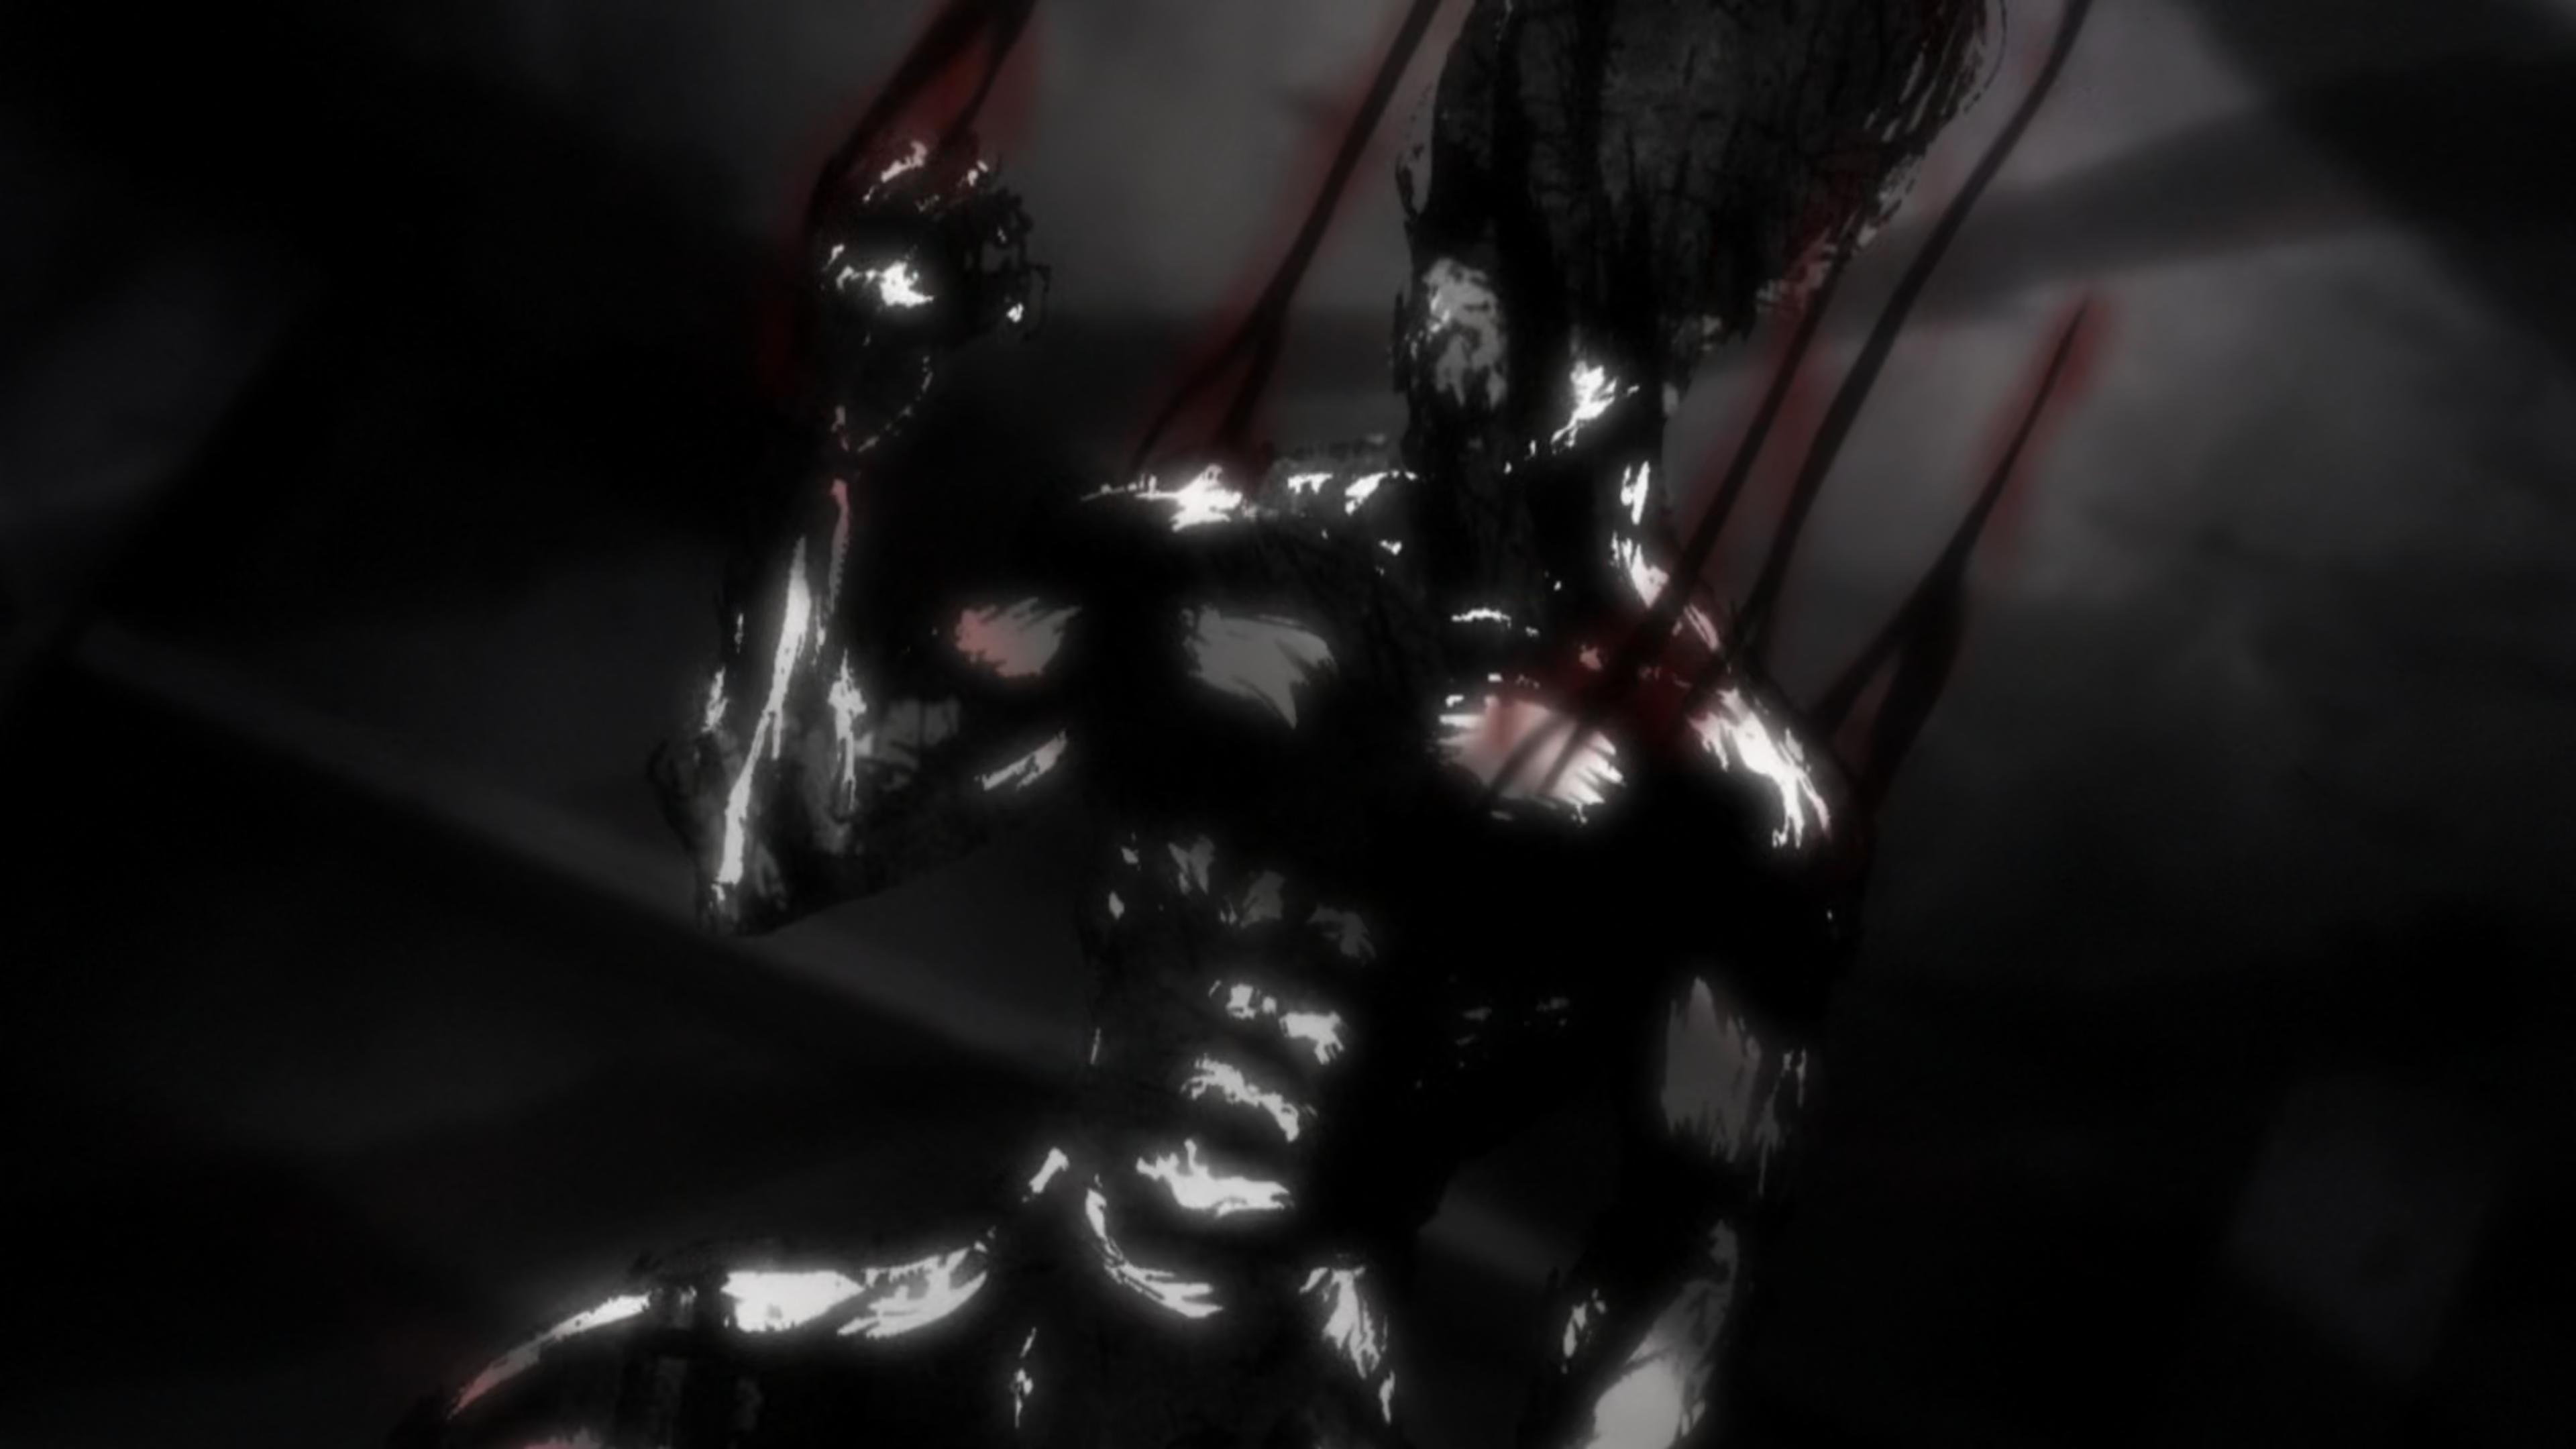
\includegraphics[width = 12cm]{Gon_berserk}
	\caption{Credit: \href{https://www.imdb.com/title/tt3748420/}{Hunter $\times$ Hunter} [S1.E131: Anger $\times$ \& $\times$ Light].}
\end{figure}

\begin{quote}
	{\sf Wrath [25]}: Tao bỏ thời gian, công sức giúp chúng mày. Lúc chúng mày đòi giúp hay kêu cứu, tao gác công việc chính sang 1 bên mà giúp đỡ không đòi hỏi. Không biết ơn tao cũng không chả thèm đòi báo ơn. Tới lúc tao hụt chân, chúng mày đạp không thương tiếc. Chưa kể còn giao việc khiến tao chồng chất công việc, khiến đầu óc mụ mị mà ảnh hưởng tới công việc chính. Chúng mày hại tao thành công rồi bay vào cắn xé không thương tiếc. Sống cái kiểu lấy oán báo ân không bằng con súc sanh. Nếu chúng mày đã không để tao sống trong bình yên mà cứ dí như con chó dại thì tao cũng chả việc gì mà phải tiếp tục nhẫn nhịn để chúng mày sống yên để hại người khác tiếp cả. Tao sẽ dùng chính cách của chúng mày làm với tao để chúng mày nếm thử mùi vị của cái ác khi mà tất cả ranh giới của sự thiện lương đã bị xóa bỏ. {\it I don't care if this is the end of mine}.
	
	{\it Why should I take pain killers, motherfuckers? Do I look like a type of kind person who needs a pain killer?} I want to be the Pain Consumer. I must be.
\end{quote}
Destroy the naive personality -- Hủy diệt nhân cách ngây thơ:
\begin{quote}
	{\sf Unknown entity [?]}: Mày làm ơn ngưng ngay trò dối gạt bản thân mình đi. Mày coi lại tổng thể cái dự án nghiên cứu này đi.
	
	{\sf Hồng [25; depressed mathematics PhD student]}: Nhưng tao mang vai trò tiên phong, tao phải chứng tỏ thực lực của tao cho họ không còn khinh thường tao, màu da của tao, hay dân tao nữa.
	
	{\sf Unknown entity [?]}: Mày nghĩ ông thầy phụ mày để mày làm tiếp sau khi mày vạch trần ổng là kẻ phá hoại nhóm à? Chưa kể ông ta còn tới mức 1 psychopath in the workplace? Sao tới tận bây giờ mà mày vẫn ngây thơ quá vậy?
	
	{\sf Hồng [25; depressed mathematics PhD student]}: Nhưng không làm Toán tiếp thì tao biết làm gì nữa?
	
	{\sf Unknown entity [?]}: Bộ mày chỉ giỏi có món đó chắc? Đừng tự dối gạt bản thân mình nữa. Mày biết điều mày muốn nhất là gì mà. Just say it clearly. Say it.
	
	{\sf Hồng [25; depressed mathematics PhD student]}: Trong sâu thẳm thâm tâm của tao, cho tới tận lúc này, tao vẫn không chắc 1 tấm bằng Tiến sĩ Toán (Mathematics PhD), dẫu thuần túy hay ứng dụng đi chăng nữa (pure or applied), có thể đo được hết khả năng của tao. Tao muốn được công nhận theo cách riêng của tao trên nhiều lĩnh vực, trong địa hạt Toán học \& cả bên ngoài địa hạt Toán học. Không phải kiểu giả làm đủ nghề như {\sc Johnny Sins}.\footnote{Diễn viên phim người lớn của Mỹ, đạo diễn, YouTuber \href{https://en.wikipedia.org/wiki/Johnny_Sins}{Wikipedia{\tt/}Johnny Sins}.} Tao muốn bất cứ thứ gì tao quan tâm \& đụng tới đều trở thành 1 dạng nghệ thuật cả, kiểu {\it Creative Artist} như nhà Toán học người Anh nổi tiếng {\sc Godfrey Harold Hardy} trong quyển {\it A Mathematician's Apology} \cite{Hardy1940,Hardy1992,Hardy2022} (tạm dịch: {\it Lời Xin Lỗi Của 1 Nhà Toán Học}) hay kiểu {\it Dilettante}\footnote{{\it dilettante}: a person who does or studies something but is not serious about it \& does not have much knowledge; a person with a general but superficial interest in any art or a branch of knowledge -- người làm hoặc nghiên cứu điều gì đó nhưng không nghiêm túc về nó \& không có nhiều kiến thức; một người có mối quan tâm chung nhưng hời hợt đối với bất kỳ nghệ thuật hoặc một nhánh kiến thức nào.} như {\sc Blaise Pascal} được mô tả trong quyển {\it Pens\'ees} \cite{Pascal_pensees} (tạm dịch: {\it Suy tư{\tt/}nghĩ}) vậy.
	
	{\sf Hồng's honesty devil [?]}: Chuẩn. Từ giờ trở đi tự mày biết phải làm gì rồi đấy.
	
	{\it``Perfectly balanced. As all things should be.''} -- {\sc Thanos}, Avenger: End Game
\end{quote}
If a human body is a physical vessel in order to contain a soul or multiple souls, then a new persona should be born. It must be. It should be contained in his physical vessel, developed from the past of being a Dark Child.
\begin{quote}
	{\sf Hồng [25; disagreeable]}: Chúng mày có cha có mẹ đầy đủ, chưa kể 1 trong 2 hoặc cả 2 người họ đều là giáo viên, mà chúng mày vẫn chưa được dạy dỗ tử tế về việc làm người \& bài học về lòng trắc ẩn, lòng thấu cảm thì để 1 đứa xuất thân từ gia đình nông dân bần hàn, mất cha sớm như tao dạy dỗ chúng mày.
	
	Nếu cả lũ chúng mày xúm tụm lại để úp sọt tao như 1 lũ Goblins bu lại giết Goblin Slayer (\href{https://www.imdb.com/title/tt8690728/}{\it Goblin Slayer} (2018--2023)) hòng giết cái phần nhân cách ngây thơ đến mức nhu nhược của tao thì cứ tự nhiên mà cắn xé. Tao sẽ xây dựng trên cái xác phần nhân cách ngây thơ đó 1 nhân cách khác đủ mạnh, thậm chí mạnh đến mức có thể diệt sạch tất cả cái phần ác của lũ Goblins chúng mày mà không cần tương tác vật lý. Hỗn chiến kiểu tác động vật lý là cho lũ con nít ranh ấu trĩ, người lớn tẩn nhau ở đấu trường của tâm trí. Chúng mày rồi sẽ phải hiểu điều đó để mà có thể trưởng thành.
\end{quote}

\subsubsection{The Room of Thought -- Căn phòng của Nghĩ Suy}
He enters the realm of Thought, totally \& completely open-minded to feel literally anything that is close to him or come towards him, like a topological object which is ready to open all of its holes, except its asshole because it is still afraid of P. Diddy, to accept anything in order to filter it.

-- Hắn bước vào địa hạt của Nghĩ Suy, hoàn toàn mở tung tâm trí để cảm nhận theo nghĩa đen bất cứ thứ gì gần hắn hay đang tiến về phía hắn, như 1 vật thể tôpô sẵn sàng dạng{\tt/}banh rộng hết tất cả các lỗ, trừ lỗ nhị do hắn vẫn khiếp sợ P. Diddy với \st{dâm} dăm 3 chai Baby Oil, để đón nhận tất cả mọi thứ để lọc chúng.

Từ khoảng 11 tuổi đến 22 tuổi, ai cũng hy vọng hắn sẽ trở nên giàu có, thành công rực rỡ, rồi quay về giúp đỡ những người dân quê, xây dựng đất nước. Ai dè đến lúc 25 tuổi, hắn bị `trầm cảm' nặng. `Trầm cảm' ở đây không phải 1 phép ví von kiểu buồn chán nặng hay giả vờ thế để thu hút sự quan tâm, thương hại từ người khác, mà là trầm cảm theo cái nghĩa chính thống của nó. Hắn cảm thấy suy nhược cơ thể \& suy nhược thần kinh. Bạn có thể phán là nếu suy nhược cơ thể thì chỉ cần ăn đầy đủ chất dinh dưỡng, kèm tập thể dục thường xuyên là sẽ trị được. Đấy là bạn chưa hiểu. That is your ignorance of how human mind actually works -- Đấy là sự thiếu hiểu biết của bạn về việc não bộ con người thực sự hoạt động như thế nào. {\it Suy nhược thần kinh mới là vấn đề cốt lõi}. Nó khiến việc suy nhược cơ thể trở nên khó trị, đúng hơn là bất trị, e.g., ăn vào ói ra hoặc không tiêu hóa được thức ăn tới nơi tới chốn mà phải thải vội ra ngoài: rối loạn tiêu hóa \& suy giảm hệ thống miễn dịch. Kiểu như cái CPU của 1 cái máy tính mà hư thì bạn có tân trang bàn phím cơ xịn xò, chuột gaming đắt tiền, đổi màn hình OLED tối tân thì cả dàn máy vẫn thế, vẫn có vấn đề, bạn phải sửa hoặc thay con CPU. Thay vì tiếp tục học Toán Cao Cấp, hay làm Khoa Học Tự Nhiên, hắn bao lấy mình bởi hàng trăm quyển sách về Tâm Lý Học (psychological books), trị liệu tâm lý (psychotherapy books), Triết Học (philosophical books), có cả các quyển về Thần Học (theology books), \& Tâm Linh (books on spirituality) nữa. Eo ơi cái thằng bé thiên phú Hội Họa \& khá giỏi Toán ngày nào. ``Tưởng giỏi lắm, tài lắm, ai dè cũng dạng hạ đẳng, chẳng thua gì súc sanh!'' Thật đáng thất vọng \& đáng bị khinh bỉ.

Thời đại học, hắn phải sống trong Ký Túc Xá với cái phòng ọp ẹp nhét 10 đứa con trai vào đấy. Từ ``phải'' ở đây do cái hoàn cảnh gia đình \& cái mớ bệnh tâm lý rối nùi của hắn. Căn phòng Ký Túc Xá không có bàn ghế -- như 1 khu ổ chuột thu nhỏ giữa Quận 1 xa xỉ giữa lòng Sài Gòn. Hắn phải mua 1 cái bàn nhựa nhỏ cho con nít, ngồi bẹp dưới sàn nhà khá bẩn, lưng dựa vào 1 thanh sắt chắn khung giường đôi. Hắn ước gì mình có 1 cái bàn đủ rộng để viết. Năm 25 tuổi, hắn từ {\sc á}o trở về căn nhà nhỏ mà cha hắn để lại cho 3 mẹ con. Trước bàn thờ của cha, mẹ hắn có mua 1 cái bàn khá rộng, mua từ tiền hắn gửi về lúc còn làm ở Đức. Hắn thích cái bàn ấy lắm, mặc dù không phải đặt ở góc phòng như kiểu nhà văn kinh dị nổi tiếng người Mỹ {\sc Stephen King} khuyên trong quyển {\it On Writing: A Memoir of the Craft} \cite{King2000,King2010}: Cái bàn gỗ của phòng thờ nhà hắn được đặt ở giữa cái phòng khách chật hẹp. Nhưng hắn thích lắm, cuối cùng cũng có 1 cái bàn đủ rộng để tha hồ viết \& sáng tạo, được ngồi bình thường để lưng không phải bị cong hay bị hằn các lằn đỏ mà thanh sắt chắn giường của Ký Túc Xá để lại lên cái lưng trần của hắn nữa. Hắn thậm chí còn không có phòng ngủ. \& hắn cảm thấy hoàn toàn ổn với điều đó. Hắn trải 1 cái chiếu, mà thật ra đa phần không cần, kế bên cái bàn vừa đủ lớn. Khi đọc sách, nghiên cứu, \& tập tành viết lách đủ mệt hoặc đôi khi ráng đến thấm mệt thì hắn lăn ngay ra ngủ. Ngủ 1 giấc thẳng cẳng, không cần biết trời trăng. Chừng nào thức dậy hắn pha cafe rồi tiếp tục ngồi vào bàn. Cuộc sống lặp đi lặp lại 1 cách đơn điệu như thế kéo dài hơn 3 năm nay. Đối với người khác thì đó là 1 cơn ác mộng kinh khủng của sự  buồn chán, đơn điệu, \& cô độc tột \st{lùn} cùng. Nhưng hắn thích điều đó. Suốt hơn 3 năm nay hắn ít ra khỏi cổng nhà, chỉ đi ra ngoài khi cần hớt tóc, mua cafe, hoặc mua các quyển sách mà không thể mua ở Tiki hoặc Shopee hoặc các nhà sách online được. 1 cuộc sống tịnh tu, nói không với các cuộc họp mặt ăn nhậu với bạn bè, \& nói không với các cuộc ân ái hoan lạc không ngừng nghỉ. \& giờ đây, sau 3 năm bế quan tu luyện, có lẽ hắn đã sẵn sàng để xuất \st{tinh} sơn. Có lẽ vậy.

\subsection{Art \& life -- Nghệ thuật \& cuộc sống}
We need arts for life. -- Chúng ta cần các dạng nghệ thuật cho cuộc sống. An advise for artists by Sir {\sc Ian McKellen}:
\begin{quotation}
	{\it``Practice any art to experience becoming. To find out what's inside you \& make your soul grow.'' -- Sir {\sc Ian McKellen} reads {\sc Kurt Vonnegut}'s inspiring letter to a group of school students.}
	
	-- Thực hành bất kỳ nghệ thuật nào để trải nghiệm sự trở thành. Để tìm ra điều gì bên trong bạn \& khiến tâm hồn bạn phát triển.'' -- Ngài {\sc Ian McKellen} đọc bức thư đầy cảm hứng của {\sc Kurt Vonnegut} gửi cho một nhóm học sinh.
\end{quotation}

\begin{quotation}
	{\it``We don't read \& write poetry because it's cute. We read \& write poetry because we are members of the human race. \& the human race is filled with passion. \& medicine, law, business, engineering, these are noble pursuits \& necessary to sustain life. But poetry, beauty, romance, love, these are what we stay alive for. To quote from Whitman, ``O me! O life! $\ldots$ of the questions of these recurring; of the endless trains of the faithless $\ldots$ of cities filled with the foolish; what good amid these, O me, O life?'' Answer. That you are here - that life exists, \& identity; that the powerful play goes on \& you may contribute a verse. That the powerful play \emph{goes on} \& you may contribute a verse. What will your verse be?''} --  {\sc N. H. Kleinbaum}, \href{https://www.imdb.com/title/tt0097165}{\it Dead Poets Society} (1989)
	
	-- Chúng ta không đọc \& viết thơ vì nó dễ thương. Chúng ta đọc \& làm thơ vì chúng ta là thành viên của loài người. \& loài người tràn đầy đam mê. \& y học, luật, kinh doanh, kỹ thuật, đây là những mục tiêu cao quý \& cần thiết để duy trì sự sống. Nhưng thơ ca, cái đẹp, sự lãng mạn, tình yêu, đó là lý do chúng ta sống sót. Để trích dẫn từ Whitman, ``Ôi tôi! Hỡi cuộc đời! $\ldots$ trong số các câu hỏi định kỳ này; về những chuyến tàu vô tận của những $\ldots$ bất tín của những thành phố đầy rẫy những kẻ ngu ngốc; Điều gì tốt đẹp giữa những điều này, ôi tôi, ôi cuộc đời?'' Trả lời. Rằng bạn đang ở đây - cuộc sống đó tồn tại, \& danh tính; rằng vở kịch mạnh mẽ sẽ tiếp tục \& bạn có thể đóng góp một đoạn thơ. Rằng vở kịch mạnh mẽ \emph{tiếp tục} \& bạn có thể đóng góp một câu thơ. Câu thơ của bạn sẽ là gì?
\end{quotation}

\begin{quote}
	{\sf Hồng [15; 10th grader]}: Năm ấy tôi giải bài Số học ẩu, sai dấu $\pm$ trong cái hằng đẳng thức $a^n\pm b^n$, nên mặc dù dư thời gian mà không chịu kiểm tra kỹ lại. Nếu mà tôi cẩn thận có khi lại Nhất toàn đoàn chứ không phải Nhì đợt Olympic 30 tháng 4 năm 2012 rồi cũng nên.
\end{quote}
2 năm sau đó, hắn ngủ quên trong chiến thắng, đã bản thân không có điều kiện tiếp xúc tài liệu tốt, các diễn đàn toán học như Mathscope \& VMF, do không có điện thoại thông minh, hay máy tính cá nhân, mà còn học tụi bạn cái thói mê gái nên hắn học hành sa sút, luôn trách cha mẹ sao không thể quan tâm hắn như cha mẹ của đám bạn cùng trang lứa lúc nào cũng lên thăm. Lý do chính là vì do hắn không nghe lời cha mẹ học gần trường gần nhà mà thi chuyên để tự thân 1 mình học xa nhà, trong khi đó, bạn Nhất toàn đoàn Olympic 30 tháng 4 năm ấy ẵm 2 Huy chương Vàng Toán Quốc Tế (International Mathematical Olympiads, abbr., IMO) nên hắn tịt mồm, không còn (dám) tiếc nữa. 10 năm sau, bạn này vẫn gặt hát thêm vô số thành công cho nền Toán học của Việt Nam:

\begin{example}[Music \& Mathematics]
	Dr. {\sc Phạm Tuấn Huy}\footnote{\href{https://scholar.google.com.vn/citations?hl=vi&user=MavyE28AAAAJ}{PTH's Google Scholar} \& \href{https://huytuanpham.github.io/}{PTH's GitHub page}. `PTH' here is the abbreviation of his name, not `Phương Trình Hàm'.} -- chàng trai vàng của làng Toán học Việt Nam trưởng thành với Âm nhạc.	
	\begin{itemize}
		\item \href{https://vnexpress.net/chang-trai-vang-toan-hoc-gianh-hoc-bong-clay-4564121.html}{VNExpress{\tt/}Chàng trai vàng Toán học giành học bổng Clay}.
		\item \href{https://vnexpress.net/nguoi-viet-doat-giai-thuong-toan-hoc-denes-k-nig-4742548.html}{VNExpress{\tt/}Người Việt đoạt giải thưởng Toán học Dénes König}.
	\end{itemize}
\end{example}

%------------------------------------------------------------------------------%

\section{Towards the $\Psi$-Flow: Optimal Experiences -- Hướng Đến Dòng Chảy Tâm Lý Học $\Psi$: Các Trải Nghiệm Tối Ưu}
\noindent\textbf{\textsf{Resources -- Tài nguyên.}}
\begin{itemize}
	\item \cite{Csikszentmihalyi_flow}. {\sc Mihaly Csikszentmihalyi}. {\it Flow: The Psychology of Optimal Experience}.
	\begin{quotation}
		{\it``The best moments usually occur when a person's body or mind is stretched to its limits in a voluntary effort to accomplish something difficult \& worthwhile. Optimal experience is thus something that we make happen.''}
		
		-- Những khoảnh khắc tuyệt vời nhất thường xảy ra khi cơ thể hoặc tâm trí của một người bị kéo căng đến giới hạn trong nỗ lực tự nguyện nhằm hoàn thành một điều gì đó khó khăn \& đáng giá. Do đó, trải nghiệm tối ưu là điều chúng ta thực hiện.
		
		{\it``The problem arises when people are so fixated on what they want to achieve that they cease to derive pleasure from the present. When that happens, they forfeit their chance of contentment.''}
		
		-- Vấn đề nảy sinh khi mọi người quá tập trung vào những gì họ muốn đạt được đến mức không còn tìm thấy niềm vui từ hiện tại. Khi điều đó xảy ra, họ mất đi cơ hội hài lòng.
		
		{\it``Enjoyment appears at the boundary between boredom \& anxiety, when the challenges are just balanced with the person's capacity to act.''}
		
		-- Sự thích thú xuất hiện ở ranh giới giữa buồn chán \& lo lắng, khi thử thách vừa đủ cân bằng với khả năng hành động của con người.		
	\end{quotation}
	Với bản dịch tiếng Việt:
	\item \cite{Csikszentmihalyi_flow_VN}. {\sc Mihaly Csikszentmihalyi}. {\it Flow: The Psychology of Optimal Experience -- Dòng Chảy: Tâm Lý Học Hiện Đại Trải Nghiệm Tối Ưu}.
\end{itemize}

\begin{definition}[$\Psi$-flow]
	``\emph{Flow} in \href{https://en.wikipedia.org/wiki/Positive_psychology}{positive psychology}, also known colloquially as being \emph{in the zone} or \emph{locked in}, is the \href{https://en.wikipedia.org/wiki/Mental_state}{mental state} in which a person performing some activity is fully immersed in a feeling of energized focus, full involvement, \& enjoyment in the process of activity. In essence, flow is characterized by the complete absorption in what one does, \& a resulting transformation in one's sense of time. Flow is the melting together of action \& \href{https://en.wikipedia.org/wiki/Consciousness}{consciousness}; the state of finding a balance between a skill \& how challenging that task is. It requires a high level of concentration. Flow is used as a \href{https://en.wikipedia.org/wiki/Coping}{coping} skill for stress \& anxiety when productively pursuing a form of leisure  that matches one's skill set.'' -- \href{https://en.wikipedia.org/wiki/Flow_(psychology)}{Wikipedia{\tt/}flow (psychology)}
\end{definition}

\begin{dinhnghia}[Dòng chảy trong tâm lý học]
	\emph{Dòng chảy} trong tâm lý học tích cực, còn được gọi thông tục là \emph{ở trong vùng} hoặc \emph{bị nhốt}, là trạng thái tinh thần trong đó 1 người thực hiện 1 số hoạt động hoàn toàn đắm chìm trong cảm giác tập trung tràn đầy năng lượng, tham gia trọn vẹn, \& thích thú trong quá trình hoạt động. Về bản chất, dòng chảy được đặc trưng bởi sự tập trung hoàn toàn vào những gì 1 người làm \& dẫn đến sự biến đổi trong nhận thức về thời gian của 1 người. Dòng chảy là sự hòa tan của sự hành động \& ý thức; trạng thái tìm kiếm sự cân bằng giữa 1 kỹ năng \& mức độ thách thức của nhiệm vụ đó. Dòng chảy đỏi hỏi mức độ tập trung cao. Dòng chảy được sử dụng như 1 kỹ năng đối phó với căng thẳng \& lo lắng khi theo đuổi 1 hình thức giải trí phù hợp với kỹ năng của 1 người 1 cách hiệu quả. 
\end{dinhnghia}

\subsection{Passion -- Niềm đam mê}

\begin{example}[{\sc Ros\'e BlackPink}]
	1 số trích dẫn hay của giọng ca chính (main vocal) Ros\'e của nhóm nhạc nữ lớn nhất Hàn Quốc hiện nay:
\end{example}
\begin{quotation}
	{\it``Life is work, \& work is life!''}
	
	-- Cuộc sống là công việc, \& công việc là cuộc sống!
	
	{\it``We grew into something that we didn't even know was possible.''}
	
	-- Chúng tôi đã phát triển thành một thứ mà chúng tôi thậm chí không biết là có thể.
	
	{\it``Singing is kind of like stress relief \& everything just kind of makes sense when I'm doing this.''}
	
	-- Ca hát giống như một cách giải tỏa căng thẳng \& mọi thứ đều trở nên có ý nghĩa khi tôi làm việc này.
	
	{\it``I'd tell myself to not feel pressure about time, that every moment you invest on watching, exploring, studying \& enjoying what you love to do, that all becomes part of becoming what you want to be.''}
	
	-- Tôi tự nhủ rằng đừng cảm thấy áp lực về thời gian, rằng mỗi khoảnh khắc bạn đầu tư vào việc quan sát, khám phá, học tập và tận hưởng những gì bạn thích làm, tất cả đều trở thành một phần của việc trở thành con người bạn muốn trở thành.
	
	{\it``Personal songs take a little more to record, definitely. We had to bring our souls into the recording studio. It was us being very vulnerable. We heard that our fans can kind of feel that.''} -- {\sc Ros\'e BlackPink}
	
	-- Chắc chắn các bài hát cá nhân cần nhiều hơn một chút để thu âm. Chúng tôi phải đem tâm hồn mình vào phòng thu âm. Đó là chúng tôi rất dễ bị tổn thương. Chúng tôi nghe nói rằng người hâm mộ của chúng tôi có thể cảm nhận được điều đó.
\end{quotation}

\begin{quote}
	{\sf Nhân [26; Ros\'e's fanboy]}: Rosé là kiểu cô gái ấm áp, dịu dàng, nhiệt tình với người khác, đầy ắp cờ xanh (full of green flags). Tôi cuồng cô idol nhỏ nhắn này tới mức có thể đợi cô ta đi ca về, sau 1 ngày cống hiến hết mình cho âm nhạc, người mệt mỏi rã rời \& nhễ nhại mồ hôi, \& rồi tôi có thể giúp cô ta làm sạch cơ thể mà không cần đến khăn lau hay nước tắm. Chỉ cô Rosé original tôi mới cuồng đến thế. Còn bất cứ ai copycat Rosé chỉ là copycat, có thể bắt chước mái tóc, vẻ bề ngoài, nhưng không bao giờ bắt chước được tính nết đáng iu, hết nước chấm đến mức muốn chấm mút hết nước của cô idol người Úc.
	
	{\sf Hồng [28; psychologist]}: Có 1 người để ngưỡng mộ, thần tượng là tốt, để giúp cuộc sống anh trở nên màu sắc \& tích cực hơn. Nhưng anh nên cân nhắc tới chuyện cai nghiện sex 1 cách nghiêm túc đi là vừa.
\end{quote}

\begin{example}[{\sc Wei Dongyi -- Vi Đông Dịch}]
	\begin{itemize}
		\item \href{https://www.mathvn.com/2021/07/wei-dongyi-thien-tai-toan-hoc-voi-ve.html}{MathVN{\tt/}{\sc Wei Dongyi} -- thiên tài toán học với vẻ ngoài `ngốc nghếch'}.
	\end{itemize}
\end{example}

%------------------------------------------------------------------------------%

\subsection{Boredom vs. Creativity -- Cơn buồn chán  vs. Sự sáng tạo}
\textbf{\textsf{Resources -- Tài nguyên.}}
\begin{itemize}
	\item \cite{Csikszentmihalyi_creativity}. {\sc Mihaly Csikszentmihalyi}. {\it Creativity: Flow \& the Psychology of Discovery \& Invention}.
	\item \cite{Pascal_pensees}. {\sc Blaise Pascal}. {\it Pens\'ees} (tạm dịch: {\it Suy nghĩ}).
\end{itemize}

\begin{quote}
	``[77] {\it Pride}. Curiosity is only vanity. We usually only want to know something so that we can talk about it; in other words, we would never travel by sea if it meant never talking about it, \& for the sheer pleasure of seeing things we could never hope to describe to others.'' -- \cite[IV. Boredom]{Pascal_pensees}
	
	-- {\it Kiêu căng, tự phụ.} Sự tò mò chỉ là sự phù phiếm. Chúng ta thường chỉ muốn biết điều gì đó để có thể nói về nó; nói cách khác, chúng ta sẽ không bao giờ đi du lịch bằng đường biển nếu điều đó có nghĩa là không bao giờ nói về nó, \& chỉ vì niềm vui tuyệt đối khi được nhìn thấy những điều mà chúng ta không bao giờ có thể hy vọng mô tả được cho người khác.
	
	``[78] {\it Description of man}. Dependence, desire for independence, needs.'' -- \cite[IV. Boredom]{Pascal_pensees}
	
	-- {\it Mô tả về con người}. Sự phụ thuộc, mong muốn độc lập, nhu cầu.
		
	``[79] How tiresome it is to give up pursuits to which we have become attached. A man enjoying a happy home-life has only to see a woman who attracts him, or spend 5 or 6 pleasant days gambling, \& he will be very sorry to go back to what he was doing before. It happens every day.'' -- \cite[IV. Boredom]{Pascal_pensees}
	
	-- Thật mệt mỏi biết bao khi phải từ bỏ những theo đuổi mà chúng ta đã gắn bó. Một người đàn ông đang tận hưởng cuộc sống gia đình hạnh phúc chỉ cần nhìn thấy một người phụ nữ thu hút anh ta, hoặc dành 5 hoặc 6 ngày vui vẻ để đánh bạc, \& anh ta sẽ rất hối hận khi quay lại công việc mình đã làm trước đây. Nó xảy ra hàng ngày.
\end{quote}

***tramdoc.vn on boredom***

%------------------------------------------------------------------------------%

\subsection{Contributions {\it\&} Legacies -- Sự cống hiến {\it\&} Di sản}

\begin{quote}
	{\sf Hồng [25; depressed mathematician wannabe]}: Nhưng tao chưa có bằng PhD, ai sẽ nghe lời tao chứ?
	
	{\sf Nhân [25; DotA2 5k mmr player]}: Mảnh bằng Tiến sĩ hay PhD chỉ là 1 minh chứng cho việc mày có khả năng nghiên cứu. Mày nên đọc bài viết \href{https://cse.buffalo.edu/~hungngo/Vietnamese/phd.html}{\it Tản mạn về mảnh bằng Ph.D}\footnote{{\sc url}: \url{https://cse.buffalo.edu/~hungngo/Vietnamese/phd.html}.} của Prof. {\sc Ngô Quang Hưng}. Cái quan trọng là việc mày cống hiến cái gì \& cống hiến như thế nào. Chẳng hạn, tao chơi DotA2 (abbr., {\it Defense of the Ancients}), 1 game 5 đấu 5. Mày nghĩ rằng chỉ có thằng carry mới được đồng đội tôn trọng à? Không, cái thằng giết nhiều địch hoặc tạo nhiều pha kiến tạo nhất -- {\it The Playmaker} -- mới là thằng khiến đồng đội của hắn tôn trọng, nể phục 1 cách tự nhiên \& nghe các chỉ thị, những lời điều binh của hắn như ``thánh chỉ'', thậm chí mày có chơi 1 con hero support ghẻ đi chăng nữa. Thằng carry hoặc mấy thằng core mà chơi ngu thì đồng đội còn khinh nữa là, nói chi nể. Cái quan trọng không phải role carry hay cores (including Carry, Midlaner, Offlaner), cái quan trọng là sự cống hiến \& tạo chiến thuật cho lối chơi của cả team, của cả tập thể mà mày đang đóng 1 vai trò chủ chốt trong đó.
\end{quote}

\begin{quotation}
	{\it``Never confuse education with intelligence. You can have a Ph.D. \& still be an idiot.''} -- {\sc Richard Feynman}
	
	-- Đừng bao giờ nhầm lẫn giáo dục với trí thông minh. Bạn có thể có bằng tiến sĩ. \& vẫn là một thằng ngốc.	
	
	{\it``When facing society, the man most concerned, the man who is to do the most \& contribute the most, has the least say.} -- \cite{Rand_fountainhead}
	
	-- Khi đối mặt với xã hội, người quan tâm nhất, người phải làm nhiều nhất \& đóng góp nhiều nhất lại là người ít nói nhất.
\end{quotation}
If you want to know more about the legendary physicists {\sc Richard Feynman}, read also:
\begin{itemize}
	\item \cite{Leighton_Feyman_last_journey}. \item \cite{Leighton_Feyman_last_journey_VN}. {\sc Ralph Leighton}. {\it Tuva or Bust! Richard Feynman's Last Journey}.
	
	Với bản dịch tiếng Việt:
	\item \cite{Leighton_Feyman_last_journey_VN}. {\sc Ralph Leighton}. {\it Tuva or Bust! Richard Feynman's Last Journey -- Cuộc Phiêu Lưu Cuối Cùng Của Feynman}.
\end{itemize}


***Aoashi***

\subsection{Convergences: Towards the endless unifications -- Các đợt hội tụ: Tiến tới các sự hợp nhất bất tận}
Walking \& thinking on the common boundaries of different domains with enough knowledge about them obtained from the corresponding divergence processes.

Dạo bước \& suy tư trên các phần biên{\tt/}ranh giới chung của các địa hạt khác nhau, với lượng kiến thức vừa đủ về các địa hạt đó thu được từ các quá trình phân kỳ tương ứng.

%------------------------------------------------------------------------------%

\section{On Research -- Bàn Về Nghiên Cứu}
\label{sect: research}

\subsection{Dirty tricks -- Các thủ đoạn bẩn thỉu}
{\it Phạm vi áp dụng.} Các thủ đoạn dưới đây cũng áp dụng trong môi trường văn phòng, \& các môi trường làm việc trong phòng kín (why?).

\noindent\textbf{\textsf{Resources -- Tài nguyên.}}
\begin{itemize}
	\item \cite{Feibelman2011}. {\sc Peter J. Feibelman}. {\it A PhD Is Not Enough!: A Guide to Survival in Science}.
	\item \cite{Phipps_Gautreys_muu_hen_ke_ban_tap_1}. {\sc Mike Phipps, Colin Gautreys}. {\it Mưu Hèn Kết Bẩn Nơi Công Sở. Tập 1: Nghệ Thuật Nhận Biết \& Phòng Tránh ``Tiểu Nhân'' Trong Công Việc}.
	\item \cite{muu_hen_ke_ban_tap_2}. Alpha Books. {\it Mưu Hèn Kết Bẩn Nơi Công Sở. Tập 2: Nghệ Thuật Thăng Tiến Trong Sự Nghiệp}.
\end{itemize}


\subsubsection{Pretend to borrow documents -- Giả vờ xin tài liệu}
1 văn phòng nghiên cứu viện Weierstrass, Berlin, Đức. Hắn thấy mình đang cặm cụi tính, chợt đồng nghiệp người Anh gốc Ấn Độ của hắn hỏi mượn tài liệu. Hắn chả nghĩ nhiều, cứ gửi qua bản tiếng Đức, kèm luôn cả bản dịch tiếng Anh mà hắn tự soạn, thêm cả ghi chú cá nhân vào đó. Hắn chợt nhớ tới chị Thương, senpai trước hắn 2 khóa, lúc hắn học Master 2. Hắn may mắn được học bổng của 1 viện nghiên cứu Pháp, Henri Lebesgue centre de math\'ematiques\footnote{\url{https://www.lebesgue.fr/en}.}. Chị ta cũng hay xin đề thi \& tài liệu của hắn. Hắn chả nghĩ nhiều nên cho mượn tuốt. Mỗi lần đưa là chỉ sẽ nói đề khó quá, có khi chỉ làm không nổi, cười mỉm, rồi sau lưng hỏi điểm từng đứa. Hắn lúc đó tự hỏi:
\begin{quote}
	{\sf Hồng [22; mathematics Master 2 student]}: Sao chỉ làm nổi nhỉ? Mình thấy chuyện hốt giải nhất Olympic sinh viên toàn quốc còn dễ chịu hơn mấy cái đề master 2 này. Toàn mánh khóe, calculus tricks đủ kiểu. Phải cày liên tục suốt vài năm mới nhớ đủ trick để làm nổi. Trong khi chỉ còn chưa biết là hàm bình phương khả tích $L^2$, thậm chí $L^p$ với $p\in[1,\infty]$, thì được không cho giá trị tại 1 vài điểm, nói đúng hơn là 1 tập có độ đo không (sets with Lebesgue measure zero). Chắc chỉ chỉ đùa cho vui. Chắc thế.
\end{quote}
Tất cả tài liệu hắn đưa cho chị ta, chỉ đều phán: ``Chị thấy cũng dễ mà.'' Hắn khá rành kiểu này, nên chỉ cười mỉm rồi cho qua. Hắn chưa bao giờ muốn gây chuyện.
\begin{quote}
	{\sf Thương [25; 2nd year mathematics PhD student in numerical analysis, sucked at mathematics]}: Chị sẽ nói thầy của tụi mình để em khỏi làm luận văn luôn.
	
	{\sf Hồng [23; mathematics Master 2 student]} nghĩ trong đầu: Đ.M. cái con khốn học dốt tới mức không biết mình dốt mà hám danh, hám quyền. Tối ngày làm mấy cái chuyện nói xấu, đâm thọt sau lưng người khác mà tỏ ra tốt đẹp. Lủng background giải tích thua cả 1 đứa licence năm nhất Đại học mà tự cho mình cái quyền đì, quyền hành xác cái thằng tự kiếm học bổng Master làm từng khâu từ làm hồ sơ {\it \'etudes en France} tới phỏng vấn {\it Campus France}. Làm bẻ mặt dân Việt Nam trước cả lớp toàn mấy thằng Pháp hệ {\it École normale supérieure} (Paris)\footnote{\href{https://en.wikipedia.org/wiki/Ecole_normale_superieure_(Paris)}{Wikipedia{\tt/}École normale supérieure (Paris)}.} (abbr., ENS). Má nó cái con khốn. {\it Fucking stupid soulless talentless eyebrowless ass-licking controlling bitch}!
\end{quote}
Đoạn, hắn im lìm, mặt cúi gầm, không chịu ngẩng lên. Mà đúng ra hắn không thể ngẩng lên. Có cái gì đó đang chết dần chết mòn \& mục rữa bên trong hắn. Không phải khối ung thư kiểu tế bào sinh học, mà là 1 loại `ung thư' khác bên trong tâm trí hắn: {\it Không giống bệnh ung thư ở thể vật lý, sinh học tế bào, bệnh trầm cảm là 1 dạng ung thư về tinh thần \& trí óc}.
\begin{quote}
	{\sf Hồng [23; mathematics Master 2 student]}: \& anh có biết điều khiến tôi vừa sợ, vừa phát điên, \& ám ảnh hơn là gì không?
	
	{\sf Hồng [27--?; psychotherapist -- nhà trị liệu tâm lý]}: Anh cứ việc nói. Tôi sẽ lắng nghe.
	
	{\sf Hồng [23; mathematics Master 2 student]}: Đó là khi tôi nhìn xung quanh cái bữa tiệc ấy, đợi ai đó cản chị ta hay nhắc khéo để ngăn cái hành động ngu xuẩn của chị ta lại. Thì ai nấy cũng nhìn tôi như cái việc tôi đáng bị như thế là hiển nhiên nhất trên trần đời. A fucking crowd of bullies. Tôi có làm gì sai chứ? Tôi chỉ tốt với sai người, \& nhẫn nhịn với nhầm người thôi mà?
\end{quote}

\subsubsection{Verbal bullying -- Bắt nạt lời nói}

\begin{quote}
	{\sf Dương [26; 2nd year mathematics PhD student in mathematical analysis, sucked at coding \& numerics]}: Mày lấy cái cứt gì mà qua được tới đây hả thằng kia?
	
	Ai thèm thuê cái chó như mày? Mẹ chả có cái chó gì cả mà xin được học bổng.
\end{quote}
Hắn chợt hiểu ra cái chuyện hắn giấu nhẹm mấy giải Olympic toán sinh viên toàn quốc là sai. Trước những đứa dốt tới mức không biết họ dốt, hắn hoàn toàn bất lực. {\it Giữ hòa khí á? Chung tay góp sức xây dựng cộng đồng đoàn kết lành mạnh á?} Pure fucking bullshits.

Dần dần, hắn căm ghét những buổi ăn chung tưởng chừng như đoàn kết nhưng toàn mấy thủ đoạn tìm điểm yếu, vạch lá tìm sâu, tỏ vẻ thông minh thượng đẳng, rồi bợ đít xu nịnh nhau như 1 lũ ô hợp. Ngồi cũng chả yên: thiên tai \& bất tài bên trái, người điên \& kẻ vô duyên bên phải.
\begin{quote}
	{\sf Hồng [23; depressed mathematics Master 2 student]}: Trừ vài người tốt bụng \& lành tính như chị Châu, anh Tuấn, anh Hợi, chị Anh ra thì toàn 1 lũ bộ tịch, lúc nào cũng tỏ vẻ bộ tịch đầy giả tạo. Mãi như những đứa con nít chưa lớn nhưng giả vờ trưởng thành để gieo rắc cái ác thuần khiết -- cái thể loại ác không biết điểm dừng của mấy đứa con nít khi làm đau người khác \& tỏ ra ngày càng thích thú khi thấy người khác ngày càng đau \& đứa con nít đó cảm thấy ngày càng có quyền lực đàn áp mọi thứ trên đường đi của chúng. 1 cái ác sơ khai, thuần khiết, non nớt không biết điểm dừng nếu không chịu bất cứ sự trừng phạt nào.
	
	{\sf Jet Black}: {\it``There's nothing as pure \& cruel as a child.''} -- \href{https://www.imdb.com/title/tt0618976}{{\it Cowboy Bebop} [S1.E20: Pierrot le Fou]} (1998--1999)
\end{quote}
-- hắn phán hệt như nhân vật chính không tên trong tiểu thuyết {\it The Catcher In The Rye} \cite{Salinger_catcher_in_rye} của {\sc Jerome David Salinger} với bản dịch tiếng Việt {\it Bắt Trẻ Đồng Xanh} \cite{Salinger_btdx}.

Từ 1 đứa cố gắng sống tốt, trở nên có ích để giúp đỡ mọi người, bất cứ ai cần giúp hắn đều sẵn sàng giúp, giờ đây hắn dần hắc hóa thành 1 kẻ khó chịu. Điều mà sau này hắn nhìn lại thì thấy đó là 1 lẽ tất yếu. Hắn phải giết chết hoặc ít nhất là hạn chế cái phần agreeable -- dễ chịu tới mức quá lành của hắn, bằng cách đặt ra ngưỡng tối đa -- maximum threshold -- thì hắn mới phát triển 1 cách lành mạnh được.

\subsubsection{Micro-envy \& micro-greedy -- Đố kỵ vi mô \& tham lam từng ly từng tý}

\begin{quote}
	{\sf Hồng [27--?; psychiatrist]}: Tại sao anh không tham gia ăn cùng với mọi người mà toàn ăn 1 mình? Những anh chị nghiên cứu sinh Tiến sĩ chắc hẳn sẽ phải đối tốt với học viên Thạc sĩ như anh mới phải lẽ chứ hả?
	
	{\sf Hồng [23; depressed mathematics Master 2 student]}: Họ hơn thua, ganh tỵ từng miếng ăn. Lúc nào tôi ăn họ cũng nhìn vào đĩa thức ăn của tôi cả. Ngắm xem miếng thịt của họ to hơn hoặc bằng miếng của tôi hay không. Nếu miếng thịt của họ to hơn thì họ tạm bằng lòng rồi khịt khịt mũi, chách lưỡi chành chạch, tằng hắng, liếc nhìn nhau kiểu thần giao cách cảm, tỏ vẻ khinh bỉ tôi. Nếu miếng thịt của họ nhỏ hơn tí xíu hoặc thực tế không hề nhỏ hơn nhưng nhận thức của họ khiến họ cảm thấy phần của họ nhỏ hơn của tôi thì họ phát tiết lên. Họ khiến tôi có cảm giác tôi không xứng đáng với đĩa thức ăn trước mặt, không xứng đáng ngồi chung với họ ở cái bàn ăn thiêng liêng chỉ dành cho những người đủ thông minh đó. Tôi mất hẳn vị giác.
	
	{\sf Hồng [27--?; psychiatrist]}: Khoan đã, ý anh nói ``miếng thịt'' là theo nghĩa bóng phải hông? Tức học bổng Master của anh?
	
	{\sf Hồng [23; depressed mathematics Master 2 student]}: Theo nghĩa đen, họ hơn thua cái miếng thịt mà nhà ăn sinh viên phát theo phần cho mỗi người.
	
	{\sf Hồng [27--?; psychiatrist]}: ``Họ'' bao nhiêu tuổi?
	
	{\sf Hồng [23; depressed mathematics Master 2 student]}: Hơn tôi 2--3 tuổi, nếu hơn 3 thì bằng tuổi chị ruột tôi. Nhưng tính tình chả khác gì những đứa con nít to xác với những cái mồm độc ác cả.
	
	{\sf Hồng [24; depressed mathematics PhD student]}: Trường hợp này cũng xảy ra với tôi. Gã người Pháp làm postdoc chung team nghiên cứu với thân hình to lớn lúc nào cũng liếc tôi cả. Mỗi lần tôi đến khu ăn chung với đồng nghiệp là hắn sẽ thét lên ``Dangerous here! Dangerous here!'' để cảnh báo tất cả đồng nghiệp chung phe với hắn hoặc những đồng nghiệp cũng cách ly hắn nhưng hắn ảo tưởng là họ chung phe bắt nạt tụi nghiên cứu sinh Tiến sĩ. Tôi nhận ra là những thành viên của đám bắt nạt cũng chả ưa gì nhau cả, toàn 1 lũ soi mói, chờ thời cơ hạ bệ lẫn nhau. Khi bị đồng nghiệp ngó lơ, bị bơ đi thì hắn sau đó trách tôi tại sao không hòa đồng, không trổ tài nấu ăn cho mọi người xem như cách hắn nướng cái bánh sinh nhật siêu khéo cho đồng nghiệp cùng thưởng thức.
	
	{\sf Hồng [27--?; psychiatrist]}: Gã người Pháp anh nói bao nhiêu tuổi?
	
	{\sf Hồng [24; depressed mathematics PhD student]}: Hơn 40 tuổi, có khi gần 50. Mà tính tình như 1 đứa con nít to xác, cũng với cái mồm ác độc.
	
	{\sf Hồng [27--?; psychiatrist]}: Thế 2 anh có nghĩ là sẽ có thể học hỏi gì từ những kẻ hơn thua miếng ăn theo nghĩa đen này không? Không, hơn thế nữa, 2 anh có nghĩ là có thể trưởng thành trong môi trường mà những kẻ này tỏ vẻ cầm trịch không?
	
	{\sf Hồng [23; depressed mathematics Master 2 student]} \& {\sf Hồng [24; depressed mathematics PhD student]}: Thế chẳng lẽ chúng tôi phải bỏ Toán mới trưởng thành được à? Chúng tôi hoàn toàn có thể hủy diệt cái sự vô học đó của bọn họ. Họ không giỏi tiếng Anh, phát âm bập bẹ không nghe rõ được, kỹ năng máy tính thì cùi bắp, kiến thức Toán của tôi lủng phần Master 1 do phân môn Giải Tích (Mathematical Analysis) đòi hỏi kiến thức nền (background) nhiều hơn hẳn các phân môn khác như Đại Số \& Thống Kê, nhưng họ thì còn tệ hơn: họ lủng cả phần Bachelor; chưa kể học đến năm 2, năm 3 nghiên cứu sinh Tiến sĩ mà không sửa được mấy cái lỗi \LaTeX\ đơn giản, trong khi chúng tôi tự học trong 1 thời gian ngắn cũng sửa trong vài phút là xong. Chúng tôi thừa sức để hủy diệt cái mồm vô học, những lời ác độc đến mất dạy của bọn họ. Nhưng chả bao giờ chúng tôi chọn cách thô lỗ \& vô học đó cả. Chúng tôi không quên rằng chúng tôi đang ở trong môi trường Hàn lâm Học thuật, đề cao tri thức \& đạo đức. Đơn giản vì bản chất con người chúng tôi không phải thế. Nếu làm thế, chúng tôi sợ sẽ biến thành những người mà chúng tôi không ưa hoặc căm ghét mất.
	
	{\sf Hồng [27--?; psychiatrist]}: Ít nhất 2 anh đi tới nơi nào đó mà có thể thưởng thức bữa ăn 1 cách trọn vẹn, không bị soi mói kích cỡ của miếng thịt trên đĩa ăn của anh nữa, thì anh mới có cảm giác ăn ngon miệng lại, lấy lại vị giác tạm thời bị mất đi. Trốn vào chốn rừng sâu để ăn beef steak như các video nấu ăn ngoài trời ở gần nơi có suối hoặc rừng rậm cũng không phải là 1 ý tồi. Bon apetit!
	
	{\sf Hồng [23; depressed mathematics Master 2 student]}: Thằng Dương còn mượn 1 tháng học bổng của tôi nữa, 1000 euro, để gom mua máy tính gì đấy. Hắn đổ thừa cái laptop của hắn. Nhưng muốn code chạy nhanh thì phải cải thiện thuật toán (algorithm) chứ, mà hắn có lương của nghiên cứu sinh mà, nhiều hơn học bổng của tôi, chắc 1700--1800 euro{\tt/}tháng trước thuế, sau thuế còn tầm 1400 euro{\tt/}tháng. Nhưng hắn bắt phải mượn của tụi Master bọn tôi.
	
	{\sf Hồng [27--?; psychiatrist]}: Nhưng tại sao anh lại cho người lạ mượn nhiều tiền đến thế?
	
	{\sf Hồng [23; depressed mathematics Master 2 student]}: Anh Tuấn học chung Master với tôi cũng hỏi y như thế. Mà tôi biết lý do rồi. 1 phần tôi muốn thân với cái nhóm các anh chị nghiên cứu sinh Tiến sĩ, có chị Phương giúp tôi các thủ tục tiếng Pháp lúc mới qua, nên tôi thấy giúp được gì giúp. Nhưng cái thằng chó này chả giúp gì tôi cả, mỗi lần đi chợ chung là hắn thó 1 vài món gì đấy từ túi đi chợ của tôi, mượn tiền mà cái giọng như cướp giật, kiểu giang hồ gangster. Mà nguyên nhân chính á? Chắc là chị Thương có lần cảnh cáo tôi là: ``Nếu em sang đây mà không chơi với ai là chết chắc đấy.'' Chơi thì chơi rồi đấy. Tặng quà, tặng đồ ăn đủ kiểu. Còn bắt phải làm cái đéo gì nữa? Cống nạp tài liệu, bóc lột công sức thì mới gọi là chơi hợp với đám bắt nạt à? Cái con khốn ngu \st{lồn} vãi linh hồn ấy. Cái thể loại gì đéo có chân mày. Xin lỗi tôi hơi xúc động, anh thông cảm.
	
	{\sf Hồng [27--?; psychiatrist]}: Không việc gì, anh cứ thành thật với cảm xúc bản thân.
	
	{\sf Hồng [23; depressed mathematics Master 2 student]}: Học thì dốt mà toàn hăm he dọa nạt tụi Master. Chả hiểu sao được sang đây học PhD. Ngay cả thầy chị ta cũng chả thể chịu nổi cái sự ngu dốt về mặt Toán học của chị ta. Chị ta than với tôi suốt là không hiểu sao chị ta ở cái tòa nhà nghiên cứu Toán lý thuyết (Pure Mathematics) đấy. Cái đó là chuyện tất yếu, chả có background thì sao làm việc ở level nghiên cứu nổi? Rồi cuối cùng thì anh biết đấy. Do không thể tự bản thân xử lý với cái mớ phức cảm tự ti (inferiority complex) mà trong tâm lý học Adler lấy làm 1 trong 2 tâm điểm nghiên cứu, bên cạnh phức cảm thượng đẳng (superiority complex), con khốn \& thằng khốn này phóng chiếu (psychological projection) tất cả những gì tự bản thân biết mình tệ hại nhưng quá hèn nhát nên không dám tự mình thừa nhận, đối diện khuyết điểm để sửa đổi \& cải thiện bản thân mà đổ thẳng lên đầu tôi. Trút sạch không sót 1 giọt độc nào. Tôi có làm gì sai chứ? Chẳng lẽ tôi phải dâng hết học bổng mà tự tôi kiếm được cho đám đó thì tụi nó mới hết cảnh cáo tôi à? Chẳng lẽ tôi phải dùng đến vũ lực như hồi năm nhất Đại học do phải ở chung với 1 thằng siêu khốn nạn ngay lúc cha tôi vừa mới mất để rồi lại bị mấy ông thầy Đại học chớp lấy \& dùng làm điểm yếu lần nữa à? Lại mấy cái chuyện giảng đạo nhảm nhí về bản tính của mấy con vật gì đấy trên kênh Discovery Channel khám phá động vật trong thiên nhiên để rồi 1 đứa tốt tánh như tôi lại phải bị ví như 1 con rắn hay 1 con sói lang nham hiểm, độc địa, ích kỷ, còn những con rắn, con sói nguy hiểm, độc ác thật sự thì lại trở thành con nai tơ ngơ ngác không biết bản thân đã làm gì mà phải mang tiếng ác à? {\it Is this how Reversed Psychology actually works?} Pure fucking bullshit.
	
	{\sf Hồng [28--?; writer]}: Đúng rồi đấy. Anh phải luyện ngữ chửi gieo vần thông minh như 1 bài rap của {\sc Eminem} vậy thì văn phong anh sẽ tiến bộ nhanh thôi.
	
	{\sf Hồng [23; depressed mathematics Master 2 student]}: Anh cút ra chỗ khác giùm tôi. Tôi đang tập trung nói chuyện với nhà trị liệu tâm lý của tôi.
	
	{\sf Hồng [27--?; psychiatrist]}: Cái sai của anh là anh không thiết lập các ranh giới lành mạnh: establish healthy boundaries.
	
	{\sf Hồng [23; depressed mathematics Master 2 student]}: Có khi phải đợi 3 năm nữa, lúc tôi bằng tuổi họ hiện giờ, tôi sẽ có cách nhìn khác.
	
	{\sf Hồng [27--?; psychiatrist]}: Thêm 1 vài năm nữa có khi anh trở thành chuyên viên trị liệu tâm lý không chừng.
\end{quote}
Hắn đeo tai nghe vào, mở gần max volume bài {\it Beautiful} của rapper huyền thoại người Mỹ {\sc Eminem} để chìm sâu vào thế giới hướng nội riêng của hắn:
\begin{multicols}{2}\it\centering
	Lately I've been hard to reach
	
	I've been too long on my own
	
	Everybody has a private world where they can be alone
	
	Are you calling me?
	
	Are you tryin' to get through?
	
	Are you reaching out for me?
	
	I'm reaching out for you
	
	[Verse 1: Eminem]
	
	I'm just so fucking depressed
	
	I just can't seem to get out this slump
	
	If I could just get over this hump
	
	But I need something to pull me out this dump
	
	I took my bruises, took my lumps
	
	Fell down then I got right back up
	
	But I need that spark to get psyched back up
	
	In order for me to pick the mic back up
	
	I don't know how or why or when
	
	I ended up in this position I'm in
	
	I'm starting to feel distant again
	
	So I decided just to pick this pen
	
	Up \& try to make an attempt
	
	To vent, but I just can't admit
	
	Or come to grips with the fact that
	
	I may be done with rap, I need a new outlet
	
	And I know some shit's so hard to swallow
	
	But I just can't sit back \& wallow
	
	In my own sorrow, but I know one fact:
	
	I'll be one tough act to follow
	
	One tough act to follow
	
	I'll be one tough act to follow
	
	Here today, gone tomorrow
	
	But you'd have to walk a thousand miles--
	
	-- {\sc Eminem}, Beautiful
\end{multicols}

\begin{Rule}[On humanity development -- Bàn về phát triển nhân cách]
	Dẫu cho bạn làm bất cứ ngành nghề nào, đừng quên nhiệm vụ chính của việc làm người là phát triển nhân cách 1 cách toàn diện. Đừng phát triển nhân cách theo xu hướng của 1 kẻ khốn nạn, thích bắt nạt bất cứ ai mà bạn cho là dưới cơ hay yếu thế hơn bạn.
\end{Rule}

\subsubsection{Steal books, delete files -- Trộm sách, xóa tập tin}

\begin{question}
	Bạn sẽ làm gì khi phát hiện bạn bè, đồng nghiệp, thậm chí là người quản lý hoặc sếp nếu làm trong môi trường công sở hoặc chính thầy{\tt/}cô, người hướng dẫn, thậm chí giáo sư nếu làm trong mảng học thuật xóa bài hoặc hủy hoại các công trình của bạn?
\end{question}

\subsubsection{Divide to control groups -- Chia rẽ khiến lục đục nội bộ để dễ dàng kiểm soát}
Thay vì phương pháp {\it chia để trị -- divide to conquer} như trong mảng {\it Bất đẳng thức -- Inequality} trong địa hạt của Toán học, phần này bàn về {\it divide to control \& micro-managing -- phương pháp chia rẽ để kiểm soát \& quản lý vi mô}.

\begin{question}
	Trong cuộc chạy đua vũ trang để mưu sinh \& để khẳng định thực lực bản thân, con người ta cần phải tốn hay phải từ bỏ 1 cách phí phạm bao nhiêu phần nhân tính tốt thuần khiết để có thể chiến thắng trên đấu trường vật chất, đấu trường vị thế, cùng nhiều thể loại đấu trường khác, bằng các phương pháp bạo lực, vô đạo đức, các thủ đoạn bẩn thỉu, hèn hạ, etc. để rồi lại thua cuộc trên đấu trường về nhân tính (humanity) \& lương tâm (conscience)?
\end{question}

\subsection{Standards -- Các tiêu chuẩn}
It is kind of funny, ironic, \& sarcastic that the 1st author of this writing is a dropout PhD student from one of the best research institutes of Applied Mathematics in Germany, Europe. Anyhow, it is also a good idea to see from the outside. The perspective of an outsider sometimes may shine some light \& reveal some insight to a dark room.

Khá là hài hước, mỉa mai, \& châm biếm khi mà tác giả đầu tiên của bài viết này lại là 1 nghiên cứu sinh bậc Tiến sĩ bỏ cuộc từ 1 trong các viện nghiên cứu tốt nhất về Toán ứng dụng của Đức. Dù gì đi nữa, cũng sẽ là 1 ý hay khi mà nhìn mọi thứ từ bên ngoài (từ tầm mắt của 1 đứa bỏ học, nghỉ việc ngang). Tầm nhìn của 1 kẻ ngoại lai đôi khi lại có thể chiếu vài tia sáng \& tiết lộ vài cái nhìn sâu sắc hay sự hiểu biết vào 1 căn phòng tối tăm. Đầu tiên chúng ta cần 1 khẩu hiệu cho cuộc diễu hành qua các dãy văn phòng u ám, hôi hám, \& tối tăm.

\vspace{2mm}
\noindent\textsf{\textbf{Slogan -- Khẩu hiệu}}: {\it A single bad publication will lead to endless public humiliations. -- Chỉ cần 1 bài báo, 1 công bố tồi cũng sẽ dẫn đến các cuộc công kích làm nhục công khai không có hồi kết}.

\begin{quote}
	{\sf Thọ [26; 3rd year theoretical mathematics PhD student]}: Anh muốn làm nghiên cứu khoa học ``thực chất'' á.
	
	{\sf Hồng [23; Master 2 student]}: Miẹ cái thằng mặt nọng với cái chất giọng ong ỏng như dư thừa Ostrogen \& thiếu hụt Testosterone.
\end{quote}
Ý ám chỉ các xuất bản mà hắn đã làm là bẩn, mà thực ra tự bản thân hắn thấy nó không đủ chuẩn như hắn mong muốn.

Hắn cũng chả hiểu anh ta cho lắm, chỉ biết nhiều anh chị lớn tuổi hơn than phiền việc bị anh này nhìn đểu. {\it Nhìn đểu là sao cơ chứ?} Thôi, không liên quan tới hắn, nên hắn cứ kệ. Mà cái kiểu đéo gì bất cứ course nào hắn học, thì anh ta đều bảo là dễ cả. {\it Dễ á?} Hắn cày muốn bụp mắt mà chưa thấy có cửa cạnh tranh với mấy anh chị ENS Paris chung lớp để điểm hắn không bị đôn xuống quá đáng. Hắn cũng để ý là ông anh này lúc nào cũng trốn ở 1 góc nào đó để rình rập \& quan sát hắn cả. {\it Tại sao cái con người lúc nào cũng tỏ ra là 1 đàn anh đáng kính với lứa đàn em đi sau, đồng thời là 1 người chồng mẫu mực, thương yêu quan tâm vợ hết mực, dẫu công việc nghiên cứu có gian khổ thế nào đi chăng nữa, lại có đặc tính của 1 kẻ rình rập (stalker) mờ ám \& nham hiểm?}

\begin{quote}
	{\sf Nhân [4--18; farmer boy]}: Nghiên cứu ``thực chất'' là như thế nào?
	
	{\sf Hồng [28--?; applied mathematician]}: Cái quan trọng là sự liên kết giữa các công trình của anh. Kiểu anh trồng 1 cái cây vậy. Cái quan trọng là anh phải giúp cho nhựa cây luồng qua mạch dẫn khắp cái cây, liên kết với nhau, i.e., các chủ đề nghiên cứu của anh phải liên kết với nhau. Nếu anh chỉ nghiên cứu những chủ đề nghiên cứu rời rạc, hoàn toàn tách xa nhau, thì cái đấy không phải trồng cây, mà là gom củi. Có thể anh sẽ tích nhặt được khá nhiều củi, lâu lâu có 1 cây củi to, hoặc được đốn từ loài gỗ quý thì anh thấy sảng khoái, vỗ ngực đùng đùng như 1 con tinh tinh kiểu xem trí khôn của ta đây [{\sc Pride}]. Nhưng nó chỉ đến thế, niềm vui của anh vẫn rời rạc, không hề có sự liên kết \& phát triển [{\sc Disappointment}], chưa kể đến sự kết nối với các cây khác trong rừng hoặc hòa trộn các nhánh nghiên cứu với nhau như phương pháp cấy ghép, chiết cành. Anh sẽ vẫn giàu nhờ tiền bán củi, nhưng sẽ không bao giờ hiểu được cái niềm vui trồng cây đúng nghĩa nếu cứ gom củi kiểu ấy.
\end{quote}

\subsection{Philosophical methodologies -- Các phương pháp luận triết học}
\textbf{\textsf{Resources -- Tài nguyên.}}
\begin{itemize}
	\item \cite{Popper_logic_science}. {\sc Karl Popper}. {\it The Logic of Scientific Discovery}.
	\item \cite{Popper_logic_khoa_hoc}. {\sc Karl Popper}. {\it The Logic of Scientific Discovery -- Logic Của Sự Khám Phá Khoa Học}.
\end{itemize}
Khi phải đối đầu với những thứ thật sự khó nhằn, hoàn toàn nằm ngoài hiểu biết hiện tại của 1 cá nhân, thì 1 cách khá đơn giản là bám víu vào những thứ đã biết rõ, dù có thể lặp đi lặp lại 1 cách đơn điệu \& nhàm chán, nhưng lại có trật tự để cân bằng với hỗn loạn -- tượng trưng cho những điều chưa biết \cite{Peterson_rule,Peterson_rule_VN,Peterson_beyond_order,Peterson_beyond_order_VN}.

\begin{example}[Cf. teaching vs. researching -- So sánh: dạy học vs. nghiên cứu]
	Dạy học bậc phổ thông trở xuống thì ``nhàn'', theo nghĩa là không cần phải nạp quá nhiều kiến thức mới, nhưng phải chú trọng về phương pháp dạy \& truyền đạt kiến thức 1 cách hiệu quả tới các học sinh. Nếu học sinh giỏi, tiếp thu nhanh thì khỏe. Gặp học sinh dốt hoặc đầu gấu thì mệt, đâm ra chán chường, cảm thấy phí phạm thời gian \& nguồn sức lực hạn chế của bản thân.
	
	Nghiên cứu thì lại khác. Trách nhiệm của nghiên cứu là phải đọc thật nhiều, nạp thật nhiều kiến thức để trau dồi bản thân mỗi ngày.***
\end{example}
Tạm phân loại học giả, theo ý cá nhân (sẽ bổ sung thêm):
\begin{itemize}
	\item Học giả làm các mảng, lĩnh vực năng động, với năng suất xuất bản ấn phẩm khoa học cao, thường được trích dẫn nhiều nhờ sự năng động của cộng đồng khoa học tương ứng.
	\item Học giả làm các mảng khó nhằn, trừu tượng, nên tần suất xuất bản ấn phẩm khoa học khá thấp, nhưng các bài này đều ở dạng nặng đô (hardcore vs. softcore), thường ít được trích dẫn vì kén độc giả. Nếu bài báo đó trở thành cornerstone thì lại được trích dẫn nhiều đến rất nhiều, na ná dạng benchmark cases for industrial purposes của loại 1 (data mẫu chuẩn để các người làm nghiên cứu R\&D ở các lĩnh vực công nghiệp dùng).
\end{itemize}
Ưu điểm của loại 1 là đi hội nghị thường xuyên. Mà đa số mấy hội nghị này giàu do dính đến công nghiệp hoặc dịch vụ số hóa (Artificial Intelligence{\tt/}Deep Learning{\tt/}Machine Learning) nên chắc đồ ăn nhiều \& ngon, ít nhất cũng ăn đứt mấy bữa tiệc giản đơn gồm trà, cafe máy cùng vài cái bánh quy như các hội nghị toán lý thuyết ở Pháp mà hồi mình học Master (hay chỉ có mấy chỗ nằm ở rìa của Pháp là vậy nhỉ?). Mà thực ra lúc mấy giáo sư Toán thảo luận với nhau, thay vì nhắm nháp cafe \& ăn bánh quy, vài người lại say xưa thảo luận mà ăn (nhầm?) phấn trắng.

Chắc mình thuộc loại 2, hoặc ít nhất là mình tự ép bản thân thuộc loại 2 (nên gọi là {\it giả học -- fake scholar} thì hợp hơn). Trong khi loại 1 thì tạo cảm giác năng động, tràn trề của sức trẻ, thì loại 2 hoàn toàn ngược lại, mà phần lớn là phải cày background khá nhiều \& nặng, \& 1 trong những cái mệt nhất nhưng rewarding nhất của loại 2 là làm các công trình khoa học liên ngành, kết nối các kết quả mạnh nhất của các lĩnh vực lý thuyết với nhau.

Có 1 bài viết phân loại học giả hay của GS. Nguyễn Tiến Zũng của ĐH Toulouse. Tiếc là sau khi GS Zũng hỗn chiến với bác  Phùng Xuân Nhạ thì website cá nhân \url{http://zung.zetamu.net/} của GS trước bị lỗi font \& giờ có lẽ đã bay màu.

\subsection{Trends \& choices -- Các xu hướng \& lựa chọn}	

\begin{quote}
	{\sf Nhân [23]}: Thế anh có biết những sở thích thời học sinh của 1 người ảnh hưởng thế nào đến xu hướng các lựa chọn chuyên ngành trong tương lai của họ không?
	
	{\sf Hồng [28]}: Tôi không rõ lắm. Cụ thể sao?
	
	{\sf Nhân [23]}: Tui sẽ lấy ví dụ về ngành Toán. Vì nó là cái duy nhất tui rành, ít hơn là rành hơn ối thứ còn lại.
	
	Những học sinh thích giải phương trình, hệ phương trình ở Toán Sơ Cấp nhưng không thích Tin học thường sẽ có xu hướng chọn các ngành lý thuyết trừu tượng, như Đại Số, Hình Học Đại Số. 
	
	Những người thích bất đẳng thức ở Toán Sơ Cấp thường sẽ có xu hướng chọn hướng Giải tích, đặc biệt là hướng Phương Trình Vi Phân Đạo Hàm Riêng (Partial Differential Equations, abbr., PDEs) vì hướng này chủ yếu đánh giá (estimation), chặn (bound), i.e., các bất đẳng thức giữa các không gian hàm. Như vậy, xu hướng thích đánh giá các đại lượng liên quan tới các hàm sơ cấp ở Toán Sơ Cấp thường sẽ phát triển thành niềm đam mê việc đánh giá các đại lượng liên quan đến hàm hoặc các đối tượng toán học trừu tượng hơn.

	1 câu hỏi điển hình của các nhà Giải tích học (mathematical analysts) khi thảo luận các vấn đề toán học liên quan đến PDEs là:
	
	- {\it Do you think it is smooth (or regular) enough? -- Anh nghĩ nó có đủ trơn (hay nhớt) không?}
	
	- {\it It seems a little rough at the initial phase. But it will be smoother later. Oh, now it's already smooth enough for us. Let's do{\tt/}play with it. -- Nhìn có vẻ hơi thô trong giai đoạn đầu (màn dạo đầu?). Nhưng rồi nó sẽ trơn hơn thôi. Ồ nhìn này, nó đủ trơn rồi kìa. Nào, chúng ta cùng xử{\tt/}quất{\tt/}chơi nó (vấn đề giải tích này) thôi}.
	
	Hàm đối tượng trơn chưa đủ, để đặt tốt 1 bài toán, miền xác định, i.e., nơi hàm đó sống, phải đủ trơn nữa, tức là cái mép (boundary $\Gamma\coloneqq\partial\Omega$) của cái miền $\Omega$ phải đủ trơn để xài các công thức tích phân từng phần (integration by parts formulas or Green's identities) để tạo ra dạng yếu (weak formulation or variational formulation). Những miền quá thô, e.g., có các góc nhọn (rough boundaries with corners), kỳ dị (singularities), chỗ nhọn dễ bị đâm (cusps), có nhiều lỗ (holes) hoặc gai (thorns) sẽ không thích hợp để làm chỗ chơi đối với các nghiệm trơn, dẫu mấy cái nghiệm đó có trơn chùi cỡ nào đi chăng nữa, vẫn không đảm bảo an toàn để chơi với chúng. Safety 1st.
	
	Ngoài lề, dù hay thắc mắc với việc đòi hỏi các nghiệm trơn, nghiệm nhớt của phương trình vi phân đạo hàm riêng có đủ trơn, đủ nhớt hay không để mà có thể vô tư chơi với chúng, tuổi thơ của các nhà giải tích cho thấy họ không có liên quan đến bất kỳ về tình dục sớm kiểu con nít quỷ hoặc sống thử, hay lạm dụng tình dục nào cả. Cho nên việc đề xuất những khẳng định kiểu như của {\sc Sigmund Freud}, e.g., các nhà toán học loay hoay với câu hỏi đủ trơn thường có tuổi thơ liên quan đến các vấn đề tình dục sớm do cha mẹ hoặc người tình của họ không quan hệ kín đáo để cho con cái vô tình bắt gặp hoặc các sang chấn tâm lý do chịu lạm dụng tình dục từ sớm; hoặc lý luận kiểu {\sc Malcolm Gladwell} trong quyển {\it Outliers: The Story of Success} \cite{Gladwell2008} hay bản dịch {\it Những Kẻ Xuất Chúng: Cái Nhìn Mới Lạ Về Nguồn Gốc Của Thành Công} \cite{Gladwell_outlier} ngụ ý việc tiếp xúc 1 cách vô thức với các từ gợi hình (gợi dục) tác động đến tiềm thức sâu bên dưới ý thức dẫn đến xu hướng chỉ thích làm với các đối tượng đủ trơn hoặc cuồng với các khái niệm đủ nhớt, etc. là hoàn toàn không có sơ sở.
	
	{\sf Hồng [28]}: {\it What is so wrong with you?}
\end{quote}

\subsection{Signs -- Các dấu hiệu}

\subsubsection{Personal systems of notations, abbreviations, \& conventions}
Bộ (tuple), tập hợp (set), hay hệ thống các ký hiệu, cách viết tắt, \& các quy ước cá nhân -- a personal set{\tt/}system of notations, abbreviations, \& conventions -- của 1 nhà khoa học tự nhiên thiên về lý thuyết hơn là về tính toán engineering thuần ứng dụng, e.g., nhà toán học (mathematicians), nhà vật lý (physicists), nhà khoa học máy tính (computer scientist), etc. là dấu hiệu đầu tiên cho biết trình độ của họ. Đơn giản vì các môn khoa học này có 1 đặc thù là đòi hỏi độ nhất quán (consistency) cực kỳ cao cho nên 1 hệ thống ký hiệu nhất quán, không mâu thuẫn, tiện dụng, không tạo ra bất kỳ sự mơ hồ, mờ mập (confusion) sẽ phản ánh phần nào trình độ của họ. Đấy là dấu hiệu dễ nhận biết đầu tiên -- nhưng còn xa so với mức phán xét -- của 1 người làm khoa học giỏi hoặc ít nhất là có 1 người thầy, người hướng dẫn giỏi.

Riêng các nhà hóa học (chemists) thì có lẽ họ được quy định chung bởi các danh pháp quốc tế như International Union of Pure \& Applied Chemistry (abbr., IUPAC)\footnote{\url{https://en.wikipedia.org/wiki/International_Union_of_Pure_and_Applied_Chemistry}.} nên không{\tt/}chưa thể dùng hệ thống ký hiệu cá nhân để đánh giá sơ bộ. Có lẽ mình nên kết thêm vài đứa bạn chuyên ngành Hóa để hiểu thêm (vừa đủ).

Thus, a good advice for young science students: Build, polish, \& perfect endlessly your personal system of notations \& conventions so well that it will fit perfectly to any of, or at least most of, your research fields. Then you can effortlessly attack each of them, connect them, play with the interaction between them \& beyond, \& even foresee the hidden structure in the realm of abstractness.

Lời khuyên (tự thân) này na ná câu trích dẫn sau của Abraham Lincoln về việc đầu tư khâu chuẩn bị kỹ lưỡng:
\begin{quote}\it
	``Give me 6 hours to chop down a tree \& I will spend the 1st 4 sharpening the axe.'' -- {\sc Abraham Lincoln} (1809--1865) -- 16th President of the United States (1861--1865)
\end{quote}

\subsubsection{Consistency -- Sự nhất quán}

\begin{question}
	Liệu có nên (dấn thân) theo 1 nghề cố định, không chịu{\tt/}thèm nhảy nghề không? 
\end{question}

\begin{figure}[H]
	\centering
	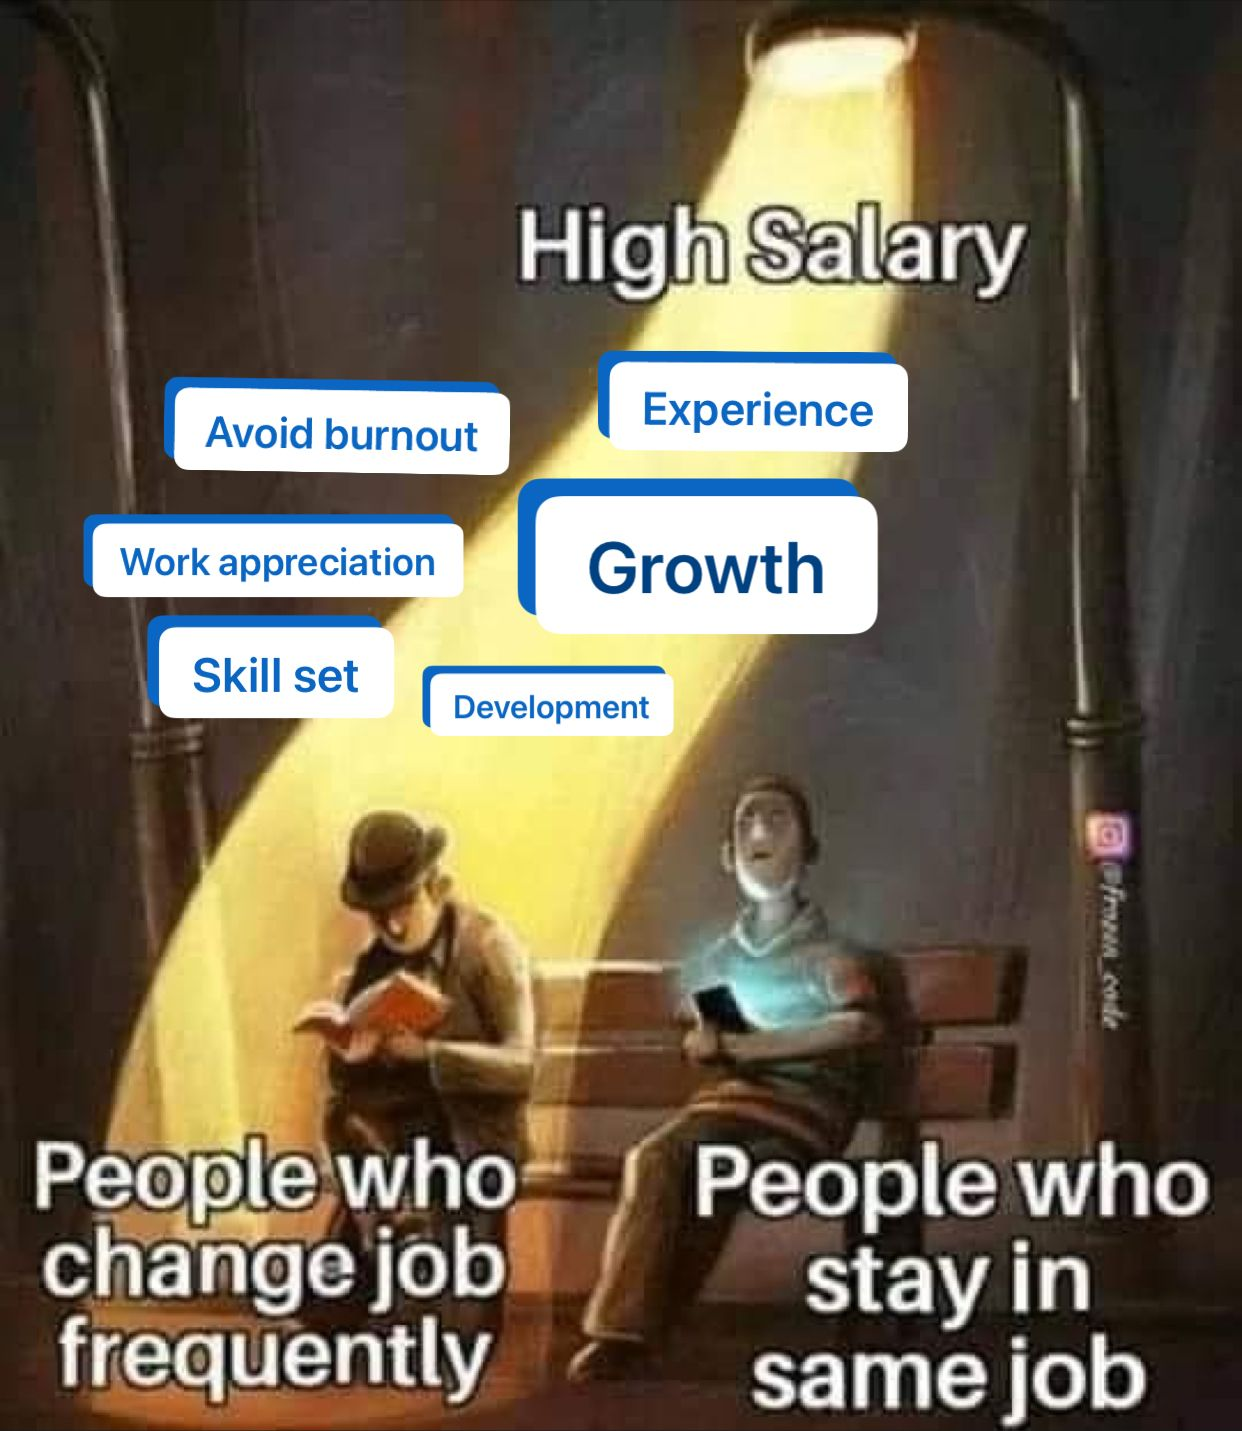
\includegraphics[width = 12cm]{high_salary}
	\caption{Credit: \href{https://www.linkedin.com/posts/judy-soloai_i-didnt-learn-this-in-school-i-learned-activity-7089014937494179840-jTze/}{Linkedin{\tt/}Judy Soloai{\tt/}I didn't learn this in school}.}
\end{figure}
Hiển nhiên 1 câu hỏi khó muôn thở. Khó chịu lẫn khó nhằn theo nhiều nghĩa. Nghĩa thứ nhất là nó không rõ ràng, \& sự không rõ ràng đến từ việc bản thân nó phụ thuộc vào quá nhiều yếu tố không thể xác định hết như các yếu tố về phương diện vật chất, e.g., lương, tài chính; cũng như các yếu tố về phương diện tinh thần, e.g., ý nghĩa công việc, cân bằng công việc--cuộc sống (work-life balance), sự phát triển cá nhân, cùng sự tương tác lẫn nhau giữa các yếu tố trong 2 phương diện đó; \& nếu lùi xa hơn nữa về quá khứ thì chúng cũng phụ thuộc vào nhiều yếu tố ban đầu của 1 cá nhân như điểm xuất phát mà bố mẹ mang lại, hoàn cảnh như khả năng tài chính của gia đình, sự ủng hộ từ dòng họ, \& ảnh hưởng của các mâu thuẫn, xung đột, lục đục nội bộ trong 2 môi trường nền tảng đó.

Tôi không hề nghĩ sẽ cố trả lời 1 cách hoàn hảo câu hỏi này hay giải quyết vấn đề này. Đồng ý là tôi ngu, nhưng chưa ngu đến mức vậy. Chưa kể có bất kỳ câu trả lời nào không (no guarantee of existence), nếu có thì cũng không hề có câu trả lời duy nhất (even if the existence is assumed, the nonuniqueness is still valid), cũng như chưa \& sẽ không chả có câu trả lời nào sẽ thỏa mãn hết tất cả các phương diện giá trị được suy xét ở {\it biểu diễn phân hoạch các giá trị \& ý nghĩa của cuộc đời} ({\it a decomposition of values \& meanings in life}) sẽ được xét đến trong Sect. \ref{sect: bullshit theory on live}: {\it A Bullshit Theory on Living -- 1 Lý Thuyết Nhảm Nhí Về Việc Sống}.

\subsubsection{Accuracy{\tt/}Precision -- Tính chính xác}

\subsubsection{Simplicity -- Sự giản đơn}
We use simplicity to fight difficulty. We do not add more unnecessary complexities \& redundancies to the war because if we do so, we will have to fight ourselves, our entanglements.

\subsubsection{Minimality -- Sự tối giản}
\noindent\textbf{\textsf{Resources -- Tài nguyên.}}
\begin{itemize}
	\item \cite{Chi2022}. {\sc Chi, Nguyễn -- The Present Writer}. {\it Một Cuốn Sách về Chủ Nghĩa Tối Giản}.
\end{itemize}

\begin{quote}
	{\sf Nhân [26--?; Jeet Kune Do practitioner -- môn sinh Tiệt Quyền Đạo]}: Ngôi sao võ thuật {\sc Bruce Lee -- Lý Tiểu Long} (tên khai sinh: {\sc Lý Chấn Phiên}) rất giỏi trong việc đưa ra cú đấm \& cú đá chuẩn xác nhất, hiệu quả nhất, với lực mạnh nhất. {\sc Lý Tiểu Long} học đủ thứ loại võ \& chọn lọc những tinh chất tốt nhất của mỗi loại võ cho riêng môn võ của ông, i.e., Tiệt Quyền Đạo (Jeet Kune Do), tinh giản đến mức tối đa. Chẳng hạn, {\sc Lý Tiểu Long} cho rằng cú đấm xoáy của Karate phí quá nhiều lực do lợi dụng việc xoáy cả cánh tay trong khi trực quyền, i.e., cú đấm thẳng, thì chuyển gần như toàn bộ lực của người ra đòn vào diện tích tiếp xúc (contact area).
	
	{\sf Hồng [25; fluid mechanics researcher -- nghiên cứu sinh Cơ Học Chất Lỏng ]}: Bản chất của điều này là do lãng phí lực phát quyền{\tt/}cước do phải truyền 1 phần vào việc xoáy (rotation) $\boldsymbol{\omega} = \operatorname{curl}{\bf v} = \operatorname{rot}{\bf v} = \nabla\times{\bf v}$ với curl\footnote{\href{https://en.wikipedia.org/wiki/Curl_(mathematics)}{Wikipedia{\tt/}curl (mathematics)}.} là toán tử vector diễn tả độ xoay hay xoáy, còn ký hiệu là rot (i.e., rotation), còn ${\bf v}$ là tốc độ của cú đấm hoặc đòn đá.
	
	{\sf Nhân [26--?; Jeet Kune Do practitioner]}: Đúng đấy, thì ra có thể hiểu được nguyên lý cú đấm của {\sc Lý Tiểu Long} theo cách nhìn của Cơ Học Chất Lỏng của Vật Lý.
	
	{\sf Hồng [25; fluid mechanics researcher]}: Nếu tôi muốn hiểu hơn về môn võ, hay đúng hơn là trường phái võ thuật này (martial art school) thì nên tìm đọc quyển nào?
	
	{\sf Nhân [26--?; Jeet Kune Do practitioner]}: Quyển {\it Tao of Jeet Kune Do} \cite{Lee2011} (tạm dịch: {\it Đạo của Tiệt Quyền Đạo}) do chính {\sc Bruce Lee} viết, tôi chưa nghiệm được tí nào.
	
	{\sf Hồng [26--?; boxing practitioner -- môn sinh đấm bốc]}: Anh có thể tham khảo thêm kỹ thuật cuộn người (body roll) để di chuyển trọng tâm cơ thể (gravity of body) để điều khiển dòng năng lượng (energy flow) vào cú đấm trong môn Quyền Anh. Nó khá là giống với bài Khởi Động cuộn 2 cánh tay di chuyển như làn sóng trong Tiệt Quyền Đạo của {\sc Lý Tiểu Long}.
	
	{\sf Hồng [25; fluid mechanics researcher]}: {\it Mục đích của 2 bài tập chuyển động cơ thể này là gì?}
	
	{\sf Nhân [26--?; Jeet Kune Do practitioner] \& Hồng [27; boxing practitioner]}: Dò tìm dòng chảy khí lực \& dòng chảy năng lượng trong cơ thể bằng độ nhạy cảm của cơ bắp \& sự tập trung tinh tế của trí óc để dồn chúng vào quyền trong môn Quyền Anh \& quyền hoặc cước trong môn Tiệt Quyền Đạo 1 cách tối ưu nhất, i.e., tiết kiệm hao phí lực, tận dụng được tối ưu chuyển động của cơ thể, độ xoay bàn chân \& cả thân người, cắt tất cả các động tác thừa thãi khiến hao phí lực không cần thiết, khiến cho gần như toàn bộ năng lượng được dồn vào đòn đánh.
	
	{\sf Hồng [25; fluid mechanics researcher]}: {\sc Lý Tiểu Long} có học Cơ Học Chất Lỏng hay không mà tự biết phải cực tiểu hóa hàm tạo bởi toán tử xoáy
	\begin{equation}
		\label{curl cost functional}
		\tag{$J_\omega$}
		J_\omega(Q_T,{\bf v}(Q_T))\coloneqq\int_0^T\int_{\Omega_t} |\nabla\times{\bf v}(t,{\bf x})|^2\,{\rm d}{\bf x}\,{\rm d}t
	\end{equation}
	với $T$ là tổng thời gian luyện tập hoặc cận chiến còn $\Omega_t$ là vùng mà người ra đòn đang chiếm lĩnh trong không gian vật lý 3 chiều $\mathbb{R}^3$ tại thời điểm $t\in[0,T]$ \& thay đổi theo thời gian $t$?
	
	{\sf Nhân [26--?; Jeet Kune Do practitioner] \& Hồng [26--?; boxing practitioner]}: Chà, ông ta là thiên tài võ thuật mà. Cần chi phải học mấy cái đó. {\sc Lý Tiểu Long} chỉ cần cảm nhận theo bản năng tự nhiên của ông ta thôi. Luyện 1 cú đá cả ngàn lần. Chỉ cần cái bộ cảm biến cơ bắp siêu nhạy cảm (highly sensitive muscle system) cùng 1 trí tuệ kiểu tư duy phản biện triết học (philosophical critical thinking) đã là quá đủ cho sự ra đời của trường phái võ thuật Jeet Kune Do. Dù là nghiên cứu sinh học thuật, nhưng anh cũng nên thử qua vài món võ thuật như Jeet Kune Do hoặc Boxing, biết đâu lại cần.
\end{quote}

\subsubsection{Critical thinking -- Tư duy phản biện}

\subsubsection{Vigor -- Khí lực, sức mãnh liệt}

\subsubsection{Rigor -- Tính chặt chẽ}

\subsubsection{Tính triệt để}

\begin{example}
	{\sc Fukuzawa Yukichi} (1834--1901) được người Nhật Bản xem như 1 trong những bậc ``khai quốc công thần'' của nước Nhật Bản hiện đại, được tôn vinh là ``Voiltaire của Nhật Bản'' vì tính triệt để, tầm mức vượt trội trong tư tưởng, \& cùng các đồng chí của ông là những người khai sáng tinh thần quốc dân Nhật Bản, đem lại linh hồn, động lực, \& sự hậu thuẫn tinh thần cho công cuộc Duy tân của chính phủ Minh Trị, với hình ảnh ông được in trên đồng tiền có mệnh giá cao nhất ở Nhật: {\rm10000 \textyen}  {\rm\cite{Yukichi_encourage_learn,Yukichi_khuyen_hoc}}.
\end{example}

\subsubsection{Obsession -- Sự ám ảnh}

\begin{quotation}\it
	``There's no talent here, this is hard work. This is an obsession. Talent does not exist, we are all equals as human beings. You could be anyone if you put in the time. You will reach the top, and that's that. I am not talented. I am obsessed.'' -- {\sc Conor McGregor}, Notorious
\end{quotation}

\begin{example}[{\sc Conor McGregor}, mixed martial artist, abbr., MMA champion weight classes]
	
\end{example}

\begin{example}[{\sc Bruce Lee}, Jeet Kune Do founder]
	
\end{example}

\begin{example}[{\sc Mike Tyson} boxer champion]
	
\end{example}

\begin{example}[{\sc David Foster Wallace} writer genius]
	
\end{example}

\subsubsection{Highly sensitive \& Sensational -- Tính nhạy cảm cao \& mức giật gân}

\begin{example}[{\sc David Foster Wallace} writer genius]
	
\end{example}

\begin{example}[{\sc Messi} football genius]
	
\end{example}

\begin{example}[{\sc Bruce Lee}, Jeet Kune Do founder]
	
\end{example}

\begin{quote}
	{\sf Nhân [15--?; nunchaku player -- người chơi côn nhị khúc]}: Khi anh thuần thạo trong việc chơi đùa với cây côn nhị khúc, i.e., sau khi anh đã bị côn đập vào các khớp xương \& đầu đủ nhiều để tự biết mà tinh chỉnh, anh không cần nhìn nữa, anh có thể cảm nhận đầu côn, moment quán tính của nó bởi cổ tay \& các sợi cơ bắp ở phần tay trước của anh. Tôi hoàn toàn có thể múa côn ở tốc độ cực cao trong bóng tối mà không phải lo bất cứ chấn thương nào cả. Có lẽ tôi đã đủ chấn thương rồi, nên đã có đủ kinh nghiệm để từ chối thêm bất cứ chấn thương nào nữa từ côn nhị khúc.
	
	{\sf Hồng [28; psychologist working on habit]}: Điều này giống việc {\sc Michael Phelps} vào vòng đua cuối của giải Olympic Bắc Kinh khi mà kính bơi của anh đầy nước khiến anh không thể thấy bất cứ thứ gì nhưng do 1 quá trình dài của việc hoàn hảo hóa các thói quen, anh có thể ``nhìn'' \& đo được đường đua bằng sải tay dài cùng cấu trúc cơ thể độc nhất vô nhị của anh khiến anh giành WR -- kỷ lục thế giới, lại vô địch 1 lần nữa. Khi bạn đã quá thành thục 1 thứ gì, nhờ thói quen, bạn đưa nó vào quá trình tự động (automatic process) của tâm trí, giúp bạn không cần suy nghĩ nữa, 1 sự thoát ly, bạn thậm chí không cần nhìn kỹ hoặc chuyển sự chú ý vào nó như trong giai đoạn đầu bạn tập luyện thứ đó nữa: {\it An automatic mental machinery \& stable effortless mental mechanism in the flow of working \& racing}.
\end{quote}

\begin{example}[{\sc Michael Phelps}]
	See {\rm\cite{Duhigg_habit}, \cite[pp. 176--184]{Duhigg_habit_VN}}.
\end{example}

\subsubsection{Integrity -- Sự chính trực}

\begin{quotation}
	{\it``Integrity is the ability to stand by an idea. That presupposes the ability to think. Thinking is something one doesn't borrow or pawn.''} -- \cite{Rand_fountainhead}
	
	-- Tính chính trực là khả năng ủng hộ một ý tưởng. Điều đó đòi hỏi khả năng suy nghĩ. Suy nghĩ là thứ người ta không mượn hay cầm đồ.
\end{quotation}

\subsubsection{Visionary -- Nhìn xa trông rộng}

%------------------------------------------------------------------------------%

\section{Dark Psychology $\boldsymbol{\Psi}$ -- Tâm Lý Học Hắc Ám $\boldsymbol{\Psi}$}

\begin{flushright}\it
	``It takes a wolf to catch a wolf.'' -- \href{https://www.imdb.com/title/tt0139654/}{Training Day} (2001)
\end{flushright}
\& it takes a wise man to catch a wolf in sheep-clothing?

\noindent\textbf{\textsf{Resources -- Tài nguyên.}}
\begin{itemize}
	\item \cite{Simon_sheep}. {\sc George Simon Jr.} {\it In Sheep's Clothing: Understanding \& Dealing with Manipulative People}.
	
	Với bản dịch tiếng Việt:
	\item \cite{Simon_sheep_VN}. {\sc George Simon Jr.} {\it In Sheep's Clothing: Understanding and Dealing with Manipulative People -- Sói Đội Lốt Cừu: Kẻ Hiếu Chiến Ngầm \& Các Thủ Thuật Thao Túng Tâm Lý}.
	
	\item \cite{Simon_character}. {\sc George Simon Jr.} {\it Character Disturbance: The Phenomenon of Our Age}.
\end{itemize}
Trước hết, để tôi giải thích cho bạn vì sao tôi lại là 1 trong những người phù hợp nhất trên cái quả đất không hề phẳng này để viết 1 cái phần có tên là {\it Dark Psychology $\boldsymbol{\Psi}$ -- Tâm Lý Học Hắc Ám $\boldsymbol{\Psi}$}. Đơn giản vì: tôi là 1 kẻ khờ -- 1 miếng mồi cực kỳ hấp dẫn đối với những kẻ có tâm lý lệch lạc.

\begin{goal}[Develop $\Psi$-manipulation draft]
	We devote this section to expand our writing: \href{https://github.com/NQBH/elementary_STEM_beyond/blob/main/learning_teaching_research/psychological_manipulation/NQBH_psychological_manipulation.pdf}{Psychological Manipulation -- Thao Túng Tâm Lý}\footnote{{\sc Nguyễn Quản Bá Hồng}. {\it Psychological Manipulation -- Thao Túng Tâm Lý}.\\{\sc url}: \url{https://github.com/NQBH/elementary_STEM_beyond/blob/main/learning_teaching_research/psychological_manipulation/NQBH_psychological_manipulation.pdf}.} written in Dec 2020, after a terrible Christmas eve, \& explain some psychological \& philosophical materials in it.
	
	-- Chúng tôi dùng phần này để mở rộng 1 bài viết cũ của chúng tôi: \href{https://github.com/NQBH/elementary_STEM_beyond/blob/main/learning_teaching_research/psychological_manipulation/NQBH_psychological_manipulation.pdf}{Psychological Manipulation -- Thao Túng Tâm Lý}, được viết hồi tháng Chạp 2020, sau 1 đêm Giáng sinh kinh hoàng.
\end{goal}

\subsection{Psychological manipulation 101 -- Thao túng tâm lý cơ bản}
\label{sect: psychological manipulation}
{\bf Keywords -- Từ khóa.} {\it Psychological manipulation -- thao túng tâm lý, psychological abuse -- lạm dụng tâm lý, emotional abuse -- lạm dụng cảm xúc, mental abuse -- lạm dụng tinh thần,  psychological violence -- bạo lực tâm lý, breaking point -- điểm gãy{\tt/}vỡ{\tt/}nguy kịch, social isolation -- cô lập xã hội, anxiety disorder -- rối loạn lo âu, depression -- trầm cảm}.

\begin{goal}[On $\Psi$-manipulation]
	Understand what ``psychological manipulation' is, why, \& how to detect \& conquer it.
	
	-- Hiểu được thao túng tâm lý là gì, tại sao thao túng tâm lý xảy ra hay tại sao ai đó lại thao túng tâm lý ai khác, \& cách phát hiện{\tt/}nhận diện \& chinh phục nó.
\end{goal}

\noindent\textbf{\textsf{Resources -- Tài nguyên.}}
\begin{itemize}
	\item \cite{Bancroft_why_he_do}. {\sc Lundy Bancroft}. {\it Why Does He Do That?: Inside the Minds of Angry \& Controlling Men}.\footnote{Amazon link: \url{https://www.amazon.com/Why-Does-He-That-Controlling/dp/0425191656}.}
	\begin{quotation}
		{\it``1 of the basic human rights he takes away from you is the right to be angry with him.''}
		
		-- 1 trong những quyền cơ bản của con người mà hắn tước đi của bạn là quyền được tức giận với hắn.
		
		{\it``Abuse \& respect are diametric opposites: You do not respect someone whom you abuse, \& you do not abuse someone whom you respect.''}
		
		-- Lạm dụng \& tôn trọng hoàn toàn trái ngược nhau: Bạn không tôn trọng người mà bạn lạm dụng, \& bạn không lạm dụng người mà bạn tôn trọng.
		
		{\it``Abuse grows from attitudes \& values, not feelings. The roots are ownership, the trunk is entitlement, \& the branches are control.''}
			
		-- Sự lạm dụng phát triển từ thái độ \& giá trị chứ không phải cảm xúc. Gốc là quyền sở hữu, thân là quyền, \& nhánh là quyền kiểm soát.
		
		{\it``Their value system is unhealthy, not their psychology.''}
		
		-- Hệ thống giá trị của họ không lành mạnh, không phải tâm lý của họ.
	\end{quotation}
	Với bản dịch tiếng Việt:
	\item \cite{Bancroft_why_he_do_VN}. {\sc Lundy Bancroft}. {\it Why Does He Do That?: Inside the Minds of Angry \& Controlling Men -- Tại Sao Anh Ta Làm Thế? Giải Mã Tâm Lý Kẻ Bạo Hành}.
	\item \cite{Bon_crowd_psychology}. {\sc Gustave Le Bon}. {\it Psychology of Crowds}.\footnote{Amazon link: \url{https://www.amazon.com/Psychology-Crowds-Gustave-Bon/dp/1907230084}.}
	
	Với bản dịch tiếng Việt:
	\item \cite{Bon_crowd_psychology_VN}. {\sc Gustave Le Bon}. {\it Psychology of Crowds -- Tâm Lý Học Đám Đông}.
	\item \cite{Braiker_string}. {\sc Harriet B. Braiker}. {\it Who's Pulling Your Strings?: How to Break the Cycle of Manipulation and Regain Control of Your Life}.
	
	Với bản dịch tiếng Việt:
	\item \cite{Braiker_string}. {\sc Harriet B. Braiker}. {\it Who's Pulling Your Strings?: How to Break the Cycle of Manipulation and Regain Control of Your Life -- Ai Đang Giật Dây Bạn?: Cách Phá Vỡ Vòng Lặp Thao Túng \& Giành Lại Quyền Kiểm Soát Cuộc Đời}.
\end{itemize}

\begin{itemize}\small\sf
	\item {\it101} [a] relating to a university course that is intended as an introduction to a subject for people who have never studied it before; relating to the basic facts in a particular field or subject.
\end{itemize}
Điển hình 1 người học Toán, đặc biệt là Đại số (Algebra) có thể thành thạo các thao tác đại số (algebraic manipulations) như cộng $+$, trừ $-$, nhân $\cdot$, chia $:$, etc., nhưng liệu người đó có chuẩn bị đủ kiến thức về mặt tâm lý để đối đầu \& phòng chống với 1 dạng manipulation khác ở 1 địa hạt khác xa hoàn toàn với địa hạt của Khoa Học Tự Nhiên nói chung \& của Toán học nói riêng, khi người đó trưởng thành \& bước vào môi trường làm việc không khi mà dạng manipulation ở địa hạt Tâm lý học không hề thuần logic \& hoàn toàn không có quy tắc hay trật tự lớp lang như manipulation của Đại số nữa: {\it A pure form of Chaos Devil}.

\begin{question}[$\psi$-manipulation]
	What is ``psychological manipulation''? Why? \& how to detect \& conquer it? -- Thao túng tâm lý là gì? Tại sao? \& làm cách nào để phát hiện cũng như chống lại nó?
\end{question}

\begin{quotation}\it
	``I just want to protect her. I don't want her to lose it. I don't want her to go through anything I went through. I don't wish that upon anybody.'' -- {\sc Justin Bieber}'s tearful interview about wanting to 'protect' {\sc Billie Eilish} from music industry resurfaces after Diddy's arrest\footnote{\href{https://www.dailymail.co.uk/news/article-13885907/justin-bieber-tearful-interview-resurface-billie-eilish-diddy-arrest.html}{DailyMail{\tt/}{\sc Justin Bieber}'s tearful interview about wanting to `protect' {\sc Billie Eilish} from music industry resurfaces after Diddy's arrest}.}
\end{quotation}
Kẻ thao túng tâm lý là kẻ tiểu nhân, nham hiểm, đê tiện. Tùy vào mức độ thao túng tâm lý thành thạo đến mức nào, mà hậu quả tâm lý, sức khỏe có thể nghiêm trọng đến ngưỡng tương đương, tùy vào sức chống chọi tâm lý \& nhận thức của nạn nhân. Các người sống sót, tạm gọi là {\it (psychological manipulated) survivor}, sau các cuộc thao túng tâm lý nặng có thể trở thành những kẻ mạnh mẽ về tâm lý \& chia sẻ cho những người đang bị thao túng tâm lý khác để có thể trở thành những người sống sót mạnh mẽ như chính họ đã từng trải qua.

\begin{definition}[Manipulation (psychology)]
	``In psychology, \emph{manipulation} is defined as an action designed to influence or control another, usually in an underhanded or unfair manner which facilitates one's personal aims. Methods someone may use to manipulate another person may include seduction, coercive control, suggestion, \href{https://en.wikipedia.org/wiki/Coercion}{coercion}, \& \href{https://en.wikipedia.org/wiki/Blackmail}{blackmail} to induce submission. Usage of the term varies depending on which behavior is specifically included, whether referring to the general population or used in clinical contexts. Manipulation is generally considered a dishonest form of \href{https://en.wikipedia.org/wiki/Social_influence}{social influences} as it is used at the expense of others.'' -- \href{https://en.wikipedia.org/wiki/Manipulation_(psychology)}{Wikipedia{\tt/}manipulation (psychology)}
\end{definition}

\begin{dinhnghia}[Thao túng tâm lý]
	Trong tâm lý học $\Psi$, \emph{thao túng} được định nghĩa là 1 hành động được thiết kế để gây ảnh hưởng hoặc kiểm soát người khác, thường theo cách thức thiếu sáng suốt hoặc không công bằng nhằm tạo điều kiện thuận lợi cho mục tiêu cá nhân của 1 người. Các phương pháp mà ai đó có thể sử dụng để thao túng người khác có thể bao gồm dụ dỗ, kiểm soát cưỡng bức, gợi ý, ép buộc, tống tiền, nhằm buộc phải phục tùng. Cách sử dụng thuật ngữ này khác nhau tùy thuộc vào hành vi nào được đưa vào cụ thể, cho dù đề cập đến dân số nói chung hay được sử dụng trong bối cảnh lâm sàng. Thao túng thường được coi là 1 hình thức không trung thực của ảnh hưởng xã hội, vì thao túng được sử dụng để gây thiệt hại cho người khác.
\end{dinhnghia}

%\begin{example}
%	``Vị sếp tuyên bố ủng hộ nhưng lại ngăn chặn mọi cơ hội tiến lên của nhân viên, tay đồng nghiệp âm thần phá hoại để giành sự ưu ái của ông chủ, người bạn đời nói yêu thương \& quan tâm nhưng dường như kiểm soát cuộc sống của người kia, ***
%\end{example}

\begin{definition}[Psychological manipulation]
	\emph{Psychological manipulation} is a type of \href{https://psychology.wikia.org/wiki/Social_influence}{social influence} that aims to change the \href{https://en.wikipedia.org/wiki/Perception}{perception} or behavior of others through underhanded, \href{https://en.wikipedia.org/wiki/Deceptive}{deceptive}, or even \href{https://psychology.wikia.org/wiki/Abuse}{abusive} tactics (\cite{Braiker_string}). By advancing only the interests of the manipulator, often at the other's expense, such methods could be considered exploitative, abusive, devious, \& deceptive.
\end{definition}

\begin{definition}[Psychological abuse{\tt/}violence, emotional{\tt/}mental abuse ]
	\emph{Psychological abuse}, often called \emph{emotional abuse}, is a form of \href{https://en.wikipedia.org/wiki/Abuse}{abuse}, characterized by a person subjecting or exposing another person to behavior that may result in \href{https://en.wikipedia.org/wiki/Psychological_trauma}{psychological trauma}, including \href{https://en.wikipedia.org/wiki/Anxiety_disorder}{anxiety}, \href{https://en.wikipedia.org/wiki/Chronic_depression}{chronic depression}, or \href{https://en.wikipedia.org/wiki/Post-traumatic_stress_disorder}{post-traumatic stress disorder} (\cite{Dutton1994,Dutton_Goodman_Bennett2000,Thompson_Kaplan1996}). It is often associated with situations of \href{https://en.wikipedia.org/wiki/Abusive_power_and_control}{power imbalance in abusive relationships}, \& may include \href{https://en.wikipedia.org/wiki/Bullying}{bullying}, \href{https://en.wikipedia.org/wiki/Gaslighting}{gaslighting}, \& \href{https://en.wikipedia.org/wiki/Workplace_bullying}{abuse in the workplace} (\cite{Dutton_Goodman_Bennett2000,Thompson_Kaplan1996}). It also may be perpetrated by persons conducting \href{https://en.wikipedia.org/wiki/Torture}{torture}, other \href{https://en.wikipedia.org/wiki/Violence}{violence}, acute or prolonged \href{https://en.wikipedia.org/wiki/Human_rights_abuse}{human rights abuse}, particularly without legal redress such as \href{https://en.wikipedia.org/wiki/Detention_without_trial}{detention without trial}, \href{https://en.wikipedia.org/wiki/False_accusation}{false accusations}, false convictions \& extreme \href{https://en.wikipedia.org/wiki/Defamation}{defamation} such as where perpetrated by state \& media. 
\end{definition}

\begin{definition}[Breaking point (psychology)]
	In human psychology, the \emph{breaking point} is a moment of \href{https://en.wikipedia.org/wiki/Stress_(medicine)}{stress} in which a person breaks down or a situation becomes critical.
\end{definition}
``The intensity of environmental stress necessary to bring this about varies from individual to individual.''

\begin{definition}[Social isolation]
	\emph{Social isolation} is a state of complete or near-complete lack of contact between an individual \& \href{https://en.wikipedia.org/wiki/Society}{society}. It differs from \href{https://en.wikipedia.org/wiki/Loneliness}{loneliness}, which reflects temporary \& involuntary lack of contact with other humans in the world. Social isolation can be an issue for individuals of any age, though symptoms may differ by age group.
\end{definition}
``Social isolation has similar characteristics in both temporary instances \& for those with a historical lifelong isolation cycle. All types of social isolation can include staying home for lengthy periods of time, having no communication with family, acquaintances or friends, and{\tt/}or willfully avoiding any contact with other humans when those opportunities do arise.''

- {\it Ừa thì đành tạm chấp nhận là mày không cố đỗ lỗi lên người khác, thế nhưng mày đang muốn nói điều gì?}

Điều mình đang muốn nói ở đây là: Trong bất kỳ mối quan hệ hay tương tác giữa người với người nào, điển hình ở đây là môi trường làm việc (workplace), khi những trải nghiệm về thực tại của bạn trở nên cực kỳ tệ \& độc hại, trái ngược hẳn với tất cả những viễn cảnh mà bạn đã \& đang mong đợi so với những gì bạn cho đi, kể cả sau khi đã tự nghi ngờ lòng tốt{\tt/}trắc ẩn lẫn kỹ năng{\tt/}thực lực của bản thân (self-doubts, imposter syndrome) đủ lâu để biết chắc rằng bạn tuyệt đối không phải là vấn đề, thì bạn cần phải hiểu một điều rằng: {\it You are not the problem. Instead, you are just another victim}$\ldots$

{\it But the victim of what? I do not understand.} Like the metaphor about the Black Hole of Truth mentioned above, the conflict between your genuine perception \& the toxic reality in any relationships (see, especially, \cite{Bancroft_why_he_do,Bancroft_why_he_do_VN}) and{\tt/}or any working environments, except the case of \href{https://en.wikipedia.org/wiki/Schizophrenia}{schizophrenia}\footnote{Tâm thần phân liệt.} of course, as a matter of fact, indicates the existence of such an invisible truth-destroyer within your environment, which is usually very close to you: {\it a psychological manipulator}$\ldots$

\begin{quotation}
	``{\it The first step in solving a problem is to recognize that it does exist}.'' - Zig Ziglar
\end{quotation}

Actually, I met \& dealt with such a person in the past, 1 year ago when I studied my Master in Pure Math in France. Ironically, although I already had some experience or thought to have it, it took me a lot of months{\tt/}efforts to detect who is the real monster in my current working environment. Sadly, I even paid a lot of trusts \& respects to that manipulator for a long time$\ldots$ Because the situation at this time is much worse for me: a psychological manipulator with a master manipulation skills in a very, very different level$\ldots$
\begin{itemize}
	\item {\it Why do, no matter how many seeds of kindness I have planted \& distributed to others, almost of them still treat me like trash{\tt/}garbage by verbally bulling, distributing toxic behaviors in return, \& even dehumanizing me?}
\end{itemize}
It seems to me that the main objective of a typical psychological manipulator is to destroy his{\tt/}her victim(s)'s confidence \& the ability to work 1st, then ruin his{\tt/}her{\tt/}(their) life later, not physically but psychologically \& mentally. However, in fact, our mental \& physical health are strongly connected \& correlated with each other. Thus, if one of them gets destroyed, then both will be shattered{\tt/}demolished{\tt/}messed up{\tt/}screwed up{\tt/}fucked up at the end anyway. \& this typical psychological manipulator seems to desire to enslave his{\tt/}her victim(s). The interesting point of this process is that it is conducted not immediately, but gradually instead. This makes sense to me. Because if someone suddenly comes to you \& forces you to form a master-slave relationship, you will certainly refuse{\tt/}deny it immediately!\footnote{Won't you?}\,\footnote{However, if that person offers you a chance to become his{\tt/}her master, the situation is far different from the one I am trying to explain here though!} That is exactly the strategy of psychological manipulators: they tighten the rope so slowly{\tt/}gently{\tt/}gradually \& carefully\footnote{Typically, they will, e.g., give some favor(s){\tt/}do some good{\tt/}kind{\tt/}nice stuff(s) whenever you seem, or they thought you seem, to start doubting them and{\tt/}or recognize their pattern of invisible destructive actions{\tt/}behaviors{\tt/}tricks.} that you cannot recognize{\tt/}detect it during a long time\footnote{Or just because I am the only sucker here, guys? {\tt .\_.} Guys?!!}. \& then one day, you become his {\tt private object}\footnote{Instead of the {\tt public class} you deserve!} without any self-awareness left - the special \& critical piece of your character which has been being tricked since a long time ago. That explains the reason why psychologists use the term ``manipulation{\tt/}manipulator'' instead of ``destruction{\tt/}destroyer'' for such kind of action{\tt/}actor{\tt/}actress in this particular context.

The relationship with a psychological manipulator is like a never-ending{\tt/}endless nightmare that no matter how hard you have been struggling to wake up, you just keep going deeper \& deeper to the rock bottom, and$\ldots$
\begin{quotation}
	``{\it I've had a lot of what I thought were rock bottoms, only to discover another, rockier bottom underneath}.'' - BoJack Horseman, {\it BoJack Horseman} (2014--2020).
\end{quotation}
Under several psychological effects of a psychological manipulator, like a black hole, everything gets sucked in \& destroyed brutally. \& even worse, that kind of person absorbs all the lights in our daily life \& then spits all darkness which each of us never wants to experience any single moment in it. All the truths are deformed{\tt/}perturbed{\tt/}twisted via the dark-magic mouth of a psychological manipulator to gradually become a germ of harsh realities in the past of somebody \& nightmare scenarios of life in his{\tt/}her future. Nothing can grow{\tt/}thrive{\tt/}flourish. The necessity to deal with this situation becomes urgent, critical, \& even vital!

{\it - I still do not understand. Your arguments do not make sense to me.}

- Daijoubu! You will understand such a thing (only) when you really suffer from it. Moreover, you should be aware of the fact that even if you do not understand something, or it does not make any sense to you, does not imply it is wrong, because: Not relative like gravity, {\it truth is absolute}.

Back to the question of dealing with a psychological manipulator: {\it What should I do then?} It seems to me at the time I write these lines that there are only 2 options to ``handle'' psychological manipulations:
\begin{enumerate}
	\item {\it Funnily enough, you can actually solve a lot of problems in your life by ignoring them!} Or,
	\item {\it You have to spot that monster{\tt/}parasite{\tt/}Shadow King (Fig. \ref{fig3}) out \& face{\tt/}fight{\tt/}deal with it.}
\end{enumerate}

\begin{figure}[H]
	\centering
	
\includegraphics[width = 12cm]{Shadow_King}
	\caption{Amahl Farouk (Shadow King), {\it Legion} (2017--2019).}
	\label{fig3}
\end{figure}
So the next question is: {\it Which option{\tt/}strategy should I choose?} My intensely personal answer is that your choice will{\tt/}should depend on your own personality trait\footnote{See also, e.g.,
	\begin{itemize}
		\item \href{https://en.wikipedia.org/wiki/Big_Five_personality_traits}{Wikipedia/Big 5 personality traits}.
		\item \href{https://en.wikipedia.org/wiki/Extraversion_and_introversion}{Wikipedia/Extraversion \& introversion}.
		\item \href{https://psychology.wikia.org/wiki/Extraversion_and_introversion}{Psychology Wiki/Extraversion \& introversion}.
		\item \href{https://psychology.wikia.org/wiki/Ambiversion}{Psychology Wiki/Ambiversion}.
		\item \href{https://www.youtube.com/watch?v=pCceO_D4AlY}{Jordan B. Peterson. 2017 Personality 14: Introduction to Traits/Psychometrics/The Big 5}.
		\item \href{https://www.youtube.com/watch?v=qYvXk_bqlBk}{Who are you, really? The puzzle of personality | Brian Little}. TED.
\end{itemize}}.
\begin{quotation}
	``{\it Life is a matter of choices, \& every choice you make makes you}.'' - John C. Maxwell
\end{quotation}
The most important question to me, in the matter of choice in life, is: {\it Are you introvert or extrovert, or in between: ambivert?}

Back to the turning point where we are trying to make a move, the former seems to be the favorite of wise human beings, meanwhile individuals with high integrity absolutely{\tt/}definitely choose the latter\footnote{Cf. Người khôn ngoan vs. kẻ chính trực - câu chuyện muôn thuở không bao giờ có hồi kết.}.

Let me assume that you have just chosen the 1st option: {\it Just ignore all the matters around you, keep working \& living happily in your own}. Sound idealistic, huh? Yeah, everything usually seems naive, simple, idealistic in the 1st glance like that$\ldots$
\begin{quotation}
	``{\it When there is no enemy within, the enemy outside can do you no harm}.'' - African proverb
	
	``{\it It's not always necessary to be strong, but to feel strong}.'' - Chris McCandless, {\it Into the Wild} (2007)
\end{quotation}
Provided you are{\tt/}feel strong inside, you do not care about psychological manipulator(s) anymore: {\it No enemy inside $\Rightarrow$ No enemy outside}. Sound perfect then! But the right{\tt/}real question is: {\it Can you always be strong{\tt/}keep being strong all the time in your life?}
\begin{quotation}
	``{\it Ups \& downs in life are very important to keep us going, because a straight line even in an ECG means we are not alive}.'' - Ratan Tata
\end{quotation}
It does not really matter you want this situation or not, you know? You have to deal with it when you already got involved. {\it Can you ignore the negative, even deadly{\tt/}fatal, effects of psychological \& emotional manipulation? Are you able to work, live, or just even breathe in that toxic atmosphere{\tt/}environment?} When you are{\tt/}feel strong enough, the ignoring-strategy seems to work effortlessly but charmingly. However, the critical point(s) is{\tt/}(are) located in the duration when you are in your downward spiral: {\it Does ignorance really help anymore?} Even assume you can ignore{\tt/}bear it a couple of times: {\it How long then}? {\it How many chances you have left before the ultimate mental breakdown comes to you?}

Furthermore, it is highly likely psychological manipulator(s) will perfectly choose your darkest time to attack \& mess your brain up: {\it A real nightmare begins} $\ldots$

It is kind of scary \& full of crazy shit, you know? Like a mind game$\ldots$ Chottomatte! No, it is actually a mind game, which should not exist in this humanity in the 1st place.

- {\it But why does this kind of redundant mind game exist in the human race?}

- Because of the term ``race'' in that phrase.

It seems that psychological manipulation is just another by-product on the \href{https://en.wikipedia.org/wiki/Human_evolution}{human evolution} at the 1st glance: {\it generally{\tt/}mostly unexpected} \& {\it unnecessary}. But look closer, think deeper: it actually can be {\it totally predicted} \& {\it absolutely unavoidable}.

Hence, this kind of mind game is compulsory{\tt/}mandatory then. The next couple of questions should be:

- {\it Do you want to play it or not (struggle or surrender)? \& if you do, how are you going to play it?}

- The answer lies in the 2nd option: {\it You must hunt them down!$\ldots$}

Let me postulate{\tt/}posit from now on the following assumption:

\begin{assumption}
	You target is to hunt the psychological manipulator(s) down in order to protect your mental health \& emotional{\tt/}physical{\tt/}psychological well-being.
\end{assumption}
So, you really want to reverse this predator-prey situation because you are too tired \& exhausted after having been being a poor prey for a long time, right? {\it How to hunt the predator back down then?}

My answer, at the moment this paragraph is written, is to think harder \& deeper \& keep questioning yourself: Because like in most predator-prey situations, you are the only person who has all the necessary pieces of the big picture. One of the simplest but most effective questions to spot out a psychological manipulator (PM, for short\footnote{But please, do not confuse this abbreviation with {\it Project Manager}, although they coincide in some situations!}) in your living{\tt/}working environment is exactly the title of the famous psychology book \cite{Bancroft_why_he_do,Bancroft_why_he_do_VN}: {\it Why does he do that?}

It seems to me the most fundamental motive of psychologically manipulative behaviors is to gain the dominance \& powers from the victims by making them suffer both mentally \& psychologically, \& then, of course, physically. 

- I am still confused, {\it why is there such a PM in our civilized society?}

- Didn't you see it yet? Because:
\begin{quotation}
	{\it Psychological manipulation is the only way to make a coward become a fucking hero!!!}$\ldots$
\end{quotation}

\begin{quotation}
	``{\it I hate weak people. Weak people$\ldots$ never fight face to face. \& poison well. Despicable. Weak people$\ldots$ They lack patience. They will quickly reap what they sow. I killed people with these `protecting fists'. I blooded my master's previous Soryuu style. I couldn't respect my father's last words. That's right. That's who I wanted to kill}.'' - Akaza, before committing suicide, Chap. 155, {\it Demon Slayer: Kimetsu No Yaiba} (2016--2020).
	
	``{\it Sometimes people try to destroy you, precisely because they recognize your power - not because they don't see it, but because they see it \& they don't want it to exist}.'' - Bell Hooks
\end{quotation}
Ironically also,

\begin{quotation}
	``{\it I see it in the people that do the real work, \& what's sad in a way is that the people that are the most giving, hardworking, \& capable of making this world better, usually don't have the ego \& ambition to be a leader}.'' - Celine, {\it Before Sunset} (2004)
	
	``{\it The world is fucked by unemotional, rational men deciding shit}.'' - Celine, {\it Before Midnight} (2013)
\end{quotation}
Let me introduce the following table to ``approximately model'' the last 2 quotes:\footnote{It will be much clearer{\tt/}more logical{\tt/}more reasonable if you add the 3rd dimension to this two-dimensional personality-trait table: \textbf{Integrity}.}

\begin{table}[h]
	\centering
	\begin{tabular}{|c|c|c|}
		\hline
		{\sc Personalities}& \textbf{Ungifted{\tt/}untalented} & \textbf{Gifted{\tt/}Talented} \\
		\hline
		\textbf{Kind{\tt/}Generous} & an ordinary but lovable giver & an ideal{\tt/}perfect leader (e.g. Hồ Chí Minh) \\
		\hline
		\textbf{Selfish{\tt/}Egocentric} & a psychological manipulator & another fucking Adolf Hitler wannabe!!! \\
		\hline
	\end{tabular}
	\caption{Some combinations of personality traits \& their associated potentially developed characters{\tt/}roles in our ``civilized'' society.}
\end{table}
{\it Nhưng ta có nên đánh giá cả một con người chỉ bằng mỗi tiêu chí rằng cá thể đó có tài hay bất tài hay không?} Nếu câu trả lời là có một cách đồng loại, thì thế giới này sẽ ngày càng trở nên thực dụng \& tình người hay sự thấu cảm rồi cũng sẽ bị phủ lên một màu xám xịt u ám \& đơn điệu$\ldots$

Thực ra thì 1 câu hỏi khác nên xuất hiện sớm hơn trước câu hỏi kiểu dehumanizing đó: {\it Chúng ta có nên đánh giá{\tt/}phán xét ai đó hay không?}
\begin{quotation}
	``{\it You know what's more destructive than a nuclear bomb?$\ldots$ Words}.'' - Kim Jong-un, {\it The Interview} (2014)
\end{quotation}
I am not trying to complicate matters here, alright? Everything is already complicated like that by its own nature. Like the mysterious but fascinating depth in the nature of anything, we cannot measure{\tt/}understand them exactly{\tt/}directly{\tt/}absolutely, we can only try our best to create models which seem reasonable enough to us to reflect partially their insights in a deeper \& clearer way$\ldots$

\begin{quotation}
	``{\it This is real life. It's not perfect, but it's real}.''\footnote{There is no ultimately complete{\tt/}perfect person, since if that person existed, he{\tt/}she would be lack of the incompleteness part(s) at least.} - Jesse, {\it Before Midnight} (2017).
\end{quotation}
Another couple of questions arises: {\it How can we understand the depth of anything in life if they are so complicated like that? Perhaps it would be much better if we stop questioning ourselves?}\footnote{``{\it Life is like riding a bicycle. To keep your balance, you must keep moving}.'' - Albert Einstein}

$\ldots$

- {\it Is this life worth living?}$\ldots$ - Yes!

- {\it Can we atone{\tt/}make amends later for all the bad{\tt/}wrong things we have done in this life after we move into the other side?}
\begin{quote}    
	BoJack Horseman: {\it ``Is it terrifying?''}
	
	Herb Kazzaz: {\it ``No. I don't think so. It's the way it is, you know? Everything must come to an end, the drip finally stops.''}
	
	BoJack Horseman: ``{\it See you on the other side}.''
	
	Herb Kazzaz: ``{\it Oh, BoJack, no, there is no other side. This is it}.'' - BoJack Horseman vs. Herb Kazzaz,  Episode: {\it The View from Halfway Down}, {\it BoJack Horseman} (2014--2020)
\end{quote}
$\ldots$ {\it Just keep thinking \& digging, deeper \& harder. There will be a day that monster will be revealed \& the hidden truth will be exposed}$\ldots$

Cuối cùng thì sau 10 tháng đầu tiên của hành trình nghiên cứu sinh đầy rẫy gian nan \& thử thách, mình cũng giải quyết được vấn đề tâm lý mà mình chịu đựng suốt thời gian qua. Chỉ tiếc là một bài toán Phổ thông nho nhỏ cho tụi học sinh Đức mà mình tự chế bị ầm thầm phá hoại \& không được published online. Tiếc là một thư mục khác trong laptop cá nhân của mình thì bị xóa (do bị ngó password lúc thảo luận mà mình không hề{\tt/}chịu đề phòng) nhằm tạo ra mâu thuẫn giữa 3 đứa PhDs cùng phòng. \& đáng tiếc là một vài đóng góp khác bị phủ nhận công sức tuyệt đối mặc dù mình đã dành nhiều tâm huyết để thực hiện (see, e.g., \cite{phill2018,Young-Powell2018}).

Nhưng giờ thì mọi thứ đã trở nên rõ ràng \& hợp lý hơn rất nhiều. Mình cũng chả trách gì, xem ra cái suất Marie--Curie này chả dễ ngốn tí nào (see the similar situation for this Marie--Curie PhD \cite{FundamentalPessimist2020}). Mình cũng đã giải thích sự tình \& hòa giải với anh bạn Đức khó tánh ở đoạn \fbox{3}, vì mình cảm nhận, thông qua vài hành động của ảnh, cả 2 thằng mình đều là những kẻ chính trực ngu ngốc, khờ dại, \& đáng thương hại. Cả 2 thằng đều bị kẻ thao túng tâm lý giở trò{\tt/}đâm thọt sau lưng, tánh ảnh nóng nên quạo, còn tánh mình hiền nên quỵ.

Ai dè cứ nói thẳng ra là mọi chuyện lại đâu vào đấy. Sau đó căng thẳng của phòng 3 đứa PhDs bọn mình cũng được giải tỏa, \& chìa khóa để giải quyết vấn đề giữa người với người (có lẽ) nằm ở lòng chân thành \& sự thấu cảm. Haizz$\ldots$ chỉ tiếc là cái CV của mình mất đi 1 dòng trong mục Referees. Nhưng vui cái là sau khi giải thích cặn kẽ sự tình với ông thầy chính ({\it real boss}) của mình, bắt đầu từ bây giờ mình sẽ được làm trực tiếp với ổng luôn. Với tại mình nói mình đã upgrade xong software trong thời gian ngắn dị thường (và chỉ ra luôn là nó chạy sai!), thành ra ổng tưởng thằng này bố láo nên bắt mình viết báo cáo! Mặc dù biết là {\it sẽ vả}\footnote{\textbf{sex var}(-iable) in {\tt Unicode/Telex}.} hơn rất nhiều vì phải báo cáo thường xuyên hơn \& phải làm một mình mà không bị ai phá, à nhầm, phụ, nhưng chỉ cần không bị đì{\tt/}kiểm soát{\tt/}thao túng nữa, là cỡ nào mình cũng ráng chơi{\tt/}quất{\tt/}tém hết! Không phải khoe, à mà khoe cũng chả sao, vì ổng là Viện trưởng, phải điều hành rất nhiều thứ nên quá bận, thành ra mới tạo cơ hội cho kẻ hám quyền lộng hành. Mọi thứ làm mình vô cùng confused trước đây cuối cùng cũng đã trở nên sáng tỏ \& hợp lý hẳn!

Nên nhớ rằng, như một phép ví von dở tệ \& làm nổi da gà, không cần biết bạn gieo bao nhiêu hạt giống tốt đẹp vào những mối quan hệ với người khác, kẻ thao túng tâm lý sẽ luôn dùng tiểu xảo{\tt/}thủ đoạn để chúng chết trước khi kịp nảy nầm, sau đó sai khiến{\tt/}thao túng khiến mọi người xung quanh trở nên kỳ thị{\tt/}xung đột \& giẫm đạp một cách tàn nhẫn lên cả bạn \& miếng vườn của bạn. Cách duy nhất để vượt qua điều này là bạn phải tìm{\tt/}săn lùng kẻ phá hoại, nếu không thì tất cả viễn cảnh tươi đẹp mà bạn hy vọng sẽ dần dần tàn lụi \& lần lượt tiêu biến, bao gồm luôn cả bạn!$\ldots$

{\it - Why were I called the Lucky Guy? Were I really lucky?}

- Yeah, I were lucky enough to experience the worst nightmare of a PhD student: the situation in which his{\tt/}her (co-)supervisor is a real master psychological manipulator who always tries to find the way to ruin his{\tt/}her work and{\tt/}or life secretly.

Nevertheless, in return, I have learned a lot from such kind of person.

\begin{quote}\it
	``A wise man can learn more from his enemies than a fool from his friends.'' -- {\sc Niki Lauda}, Rush (2013)
\end{quote}
Love, trust, \& respect are so special. I cannot force{\tt/}manipulate anyone to give these things to me for free: Honestly, I do not have any right to do that \& these things actually need {\it building{\tt/}giving}, instead of {\it forcing{\tt/}taking}$\ldots$ {\it The harder you force someone to love{\tt/}trust{\tt/}respect you, the stronger{\tt/}deeper they hate{\tt/}distrust (mistrust){\tt/}disgust (disrespect) you instead.}

{\it It is all about a well-deserved victory indeed} $\ldots$

\subsubsection{{\color{gray}/* Quick sketches */}}
\fbox{\textbf{13}} I have been using \href{https://github.com}{GitHub} during the beginning of my PhD journey. It seems to me at this moment that \href{https://git-scm.com/}{git} is a perfect tool for blogging! This {\tt git add-commit-push} working style is so perfect to motivate me \& push my workflow in a more disciplined way, which is highly suitable for an undisciplined shitty person like me.

{\it - How many commits have you attempted to push your limit today, man?}

- {\it You mean suicide?} Yeah$\ldots$ a couple of times.

- No, WTF, dude! I mean commit in the {\tt git} sense. {\it What's wrong with your brain, bruh?}

{\it - Why did you remove a necessary supervision from your PhD journey? Don't you want another Vietnamese to be able to get this kind of ``prestigious'' fellowship?}

\begin{quote}
	``{\it I can't concentrate. I can still hear the sound of the piano. It's in my way. You're in my way, so$\ldots$ Get out of here!}'' - Arima Kousei, {\it Your Lie in April}  (2014--2015).
\end{quote}

- No, I did that because I really want it (Fig. \ref{fig4}).
\begin{figure}[H]
	\centering
	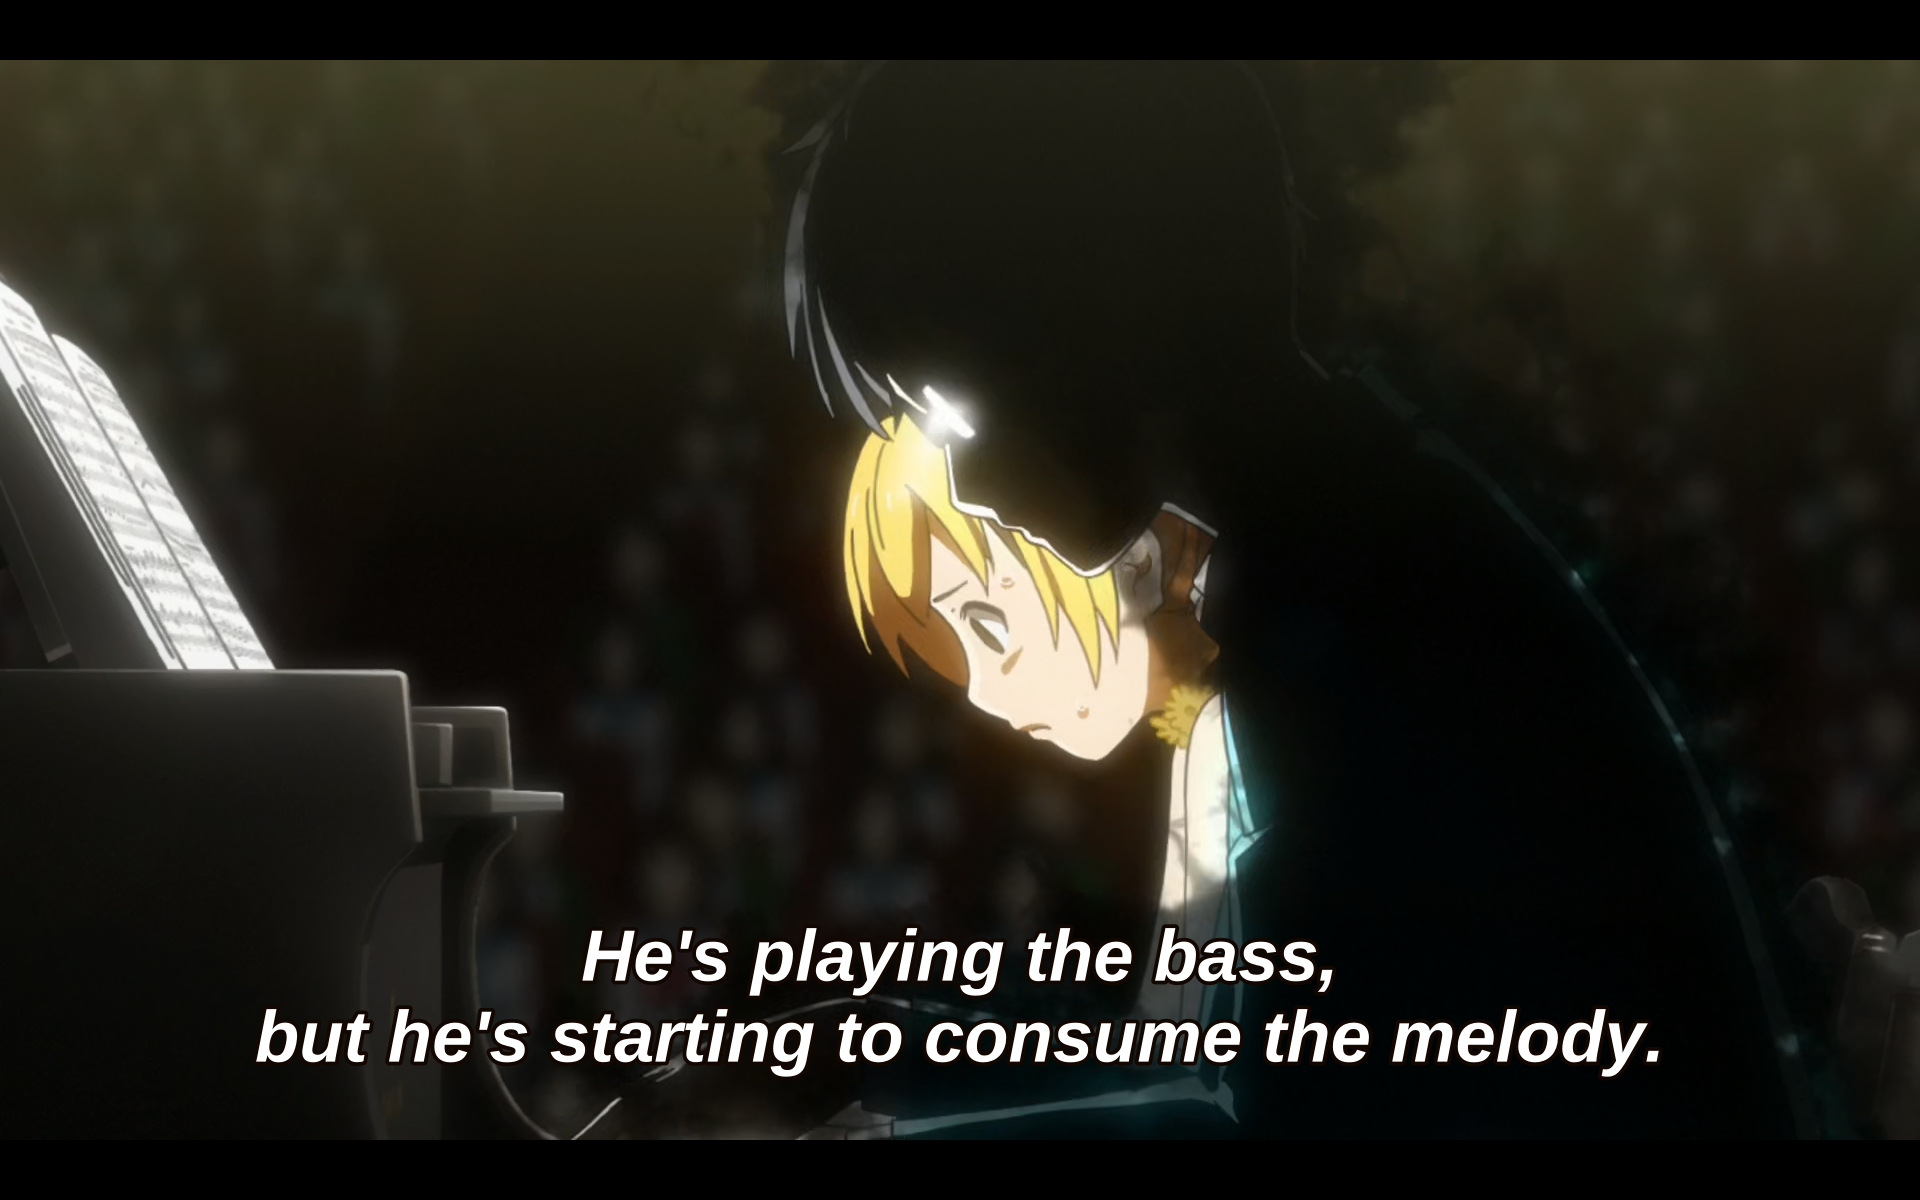
\includegraphics[width = 12cm]{Arima_Kousei_emotional_explosion}
	\caption{Arima Kousei's emotional explosion, {\it Your Lie in April} (2014--2015).}
	\label{fig4}
\end{figure}

{\it - Do you feel ashamed of that?}

\begin{quote}
	``{\it It doesn't matter where you are, it's who you are, that's not gonna change whether you're in California or Maine or New Mexico. You know, you can't escape you}.'' - Penny Carson, {\it BoJack Horseman} (2014--2020)
\end{quote}

- At the moment when you admit that you are stupid, you have eliminated a lot of inner sources of fear\footnote{\href{https://www.youtube.com/watch?v=bb9g9mtDHZo}{How To Beat Fear \& Anxiety | Jordan Peterson | Powerful Life Advice}.} \& shame from yourself: {\it You escaped you}.

{\it - But what if you fail then?}

- {\it Then what? So what?} As long as I have already tried the best of myself, nothing else matters $\ldots$

{\it - Is this world a place for good{\tt/}kind people?}

- No, it is the place for all people, particularly good{\tt/}kind people, but the problem is: if you are, especially, a good person, you have to struggle to protect yourself from the other predators. {\it Do you want to be a prey, which sounds similar to ``afraid'', all your life?} 

My mom used to teach me that if I do good things to other people, they will definitely give good things back. {\it But is this true?} I doubt it. This human race makes me doubt it. However, the question following that one should not be like: {\it Should I become a good{\tt/}kind person or not?} Instead, it should be: {\it I definitely want to be a good{\tt/}kind person, but good{\tt/}kind with whom?}

Like the working principle of {\tt git}, we will encounter a lot of complicated events{\tt/}situations{\tt/}troubles in our life, \& for each of them, we have our own list of choices{\tt/}options, like {\tt branches}. At each turning point, we are able to develop several different future versions of ourselves, of our personality, \& this also affects a lot to our action{\tt/}reaction{\tt/}behaviors{\tt/}character in future.

{\it Then which set of choices is the best? Which branch is the optimal?} Nobody knows the answer (right?). We have to choose according to our considerations{\tt/}perceptions, which are usually based on our own experiences, at that very moment. If that choice works, it will become background{\tt/}fundamental (sometimes self-delusion!) step for the next turning point. \& if it does not, we also have an additional experience for the next turn instead. {\it Nothing is absolutely good or bad, just our perception towards a particular event{\tt/}idea{\tt/}problem{\tt/}situation.}

It seems to me that individuals with high integrity usually attracts mysteriously a lot of troubles, especially in social relationships. So I call each of them, including myself, a ``drama-magnet''.

\begin{quotation}
	``{\it Nhưng cũng có lúc mọi thứ không như là những gì ta muốn. Thế giới này vận hành theo cái cách luôn ghì ta xuống}.'' - Đen Vâu, {\it Bài này chill phết} (2019)
	
	``{\it You pray for rain, you gotta deal with the mud too. That's part of the deal}.'' - Denzel Washington
\end{quotation}
Do not blame yourself as a drama-magnet, you should be proud of it instead!
\\

- Mà bạn êi, bạn nghiên cứu sinh ngành toán sao không lo học toán, mà đi đọc mấy cái tâm lý này chi cho phí thời gian vại?

- À, là vì toán \& tâm lý là 2 ngành học dễ gây trầm cảm nhất, cộng với việc chuyên ngành của mình là toán nữa, nên mình cày luôn tâm lý cho đủ bộ!

- Sugoiii!!!

\subsubsection{{\tt {\color{RubineRed}return} {\color{Purple}<?>}; \}}}
{\tt \small You expect this text to return what?} {\tt 0?}

\paragraph{{\it Emotions}: good{\tt/}bad? {\it Emotionless?}}
\noindent
\fbox{\textbf{17}} We start loving something{\tt/}someone, or being attracted by something{\tt/}someone, because that thing{\tt/} person seems to give us a lot of energy{\tt/}happiness{\tt/}emotions\footnote{E.g., music, movie, sport, subject, relationship, career, etc.} and{\tt/}or reduce{\tt/}release our pain{\tt/}suffering\footnote{E.g., lyrics, sex, alcohol, drugs, etc.}. But after playing with it{\tt/}him{\tt/}her, consuming it{\tt/}him{\tt/}her for a while, we get bored, we find another one, a new source of emotion generators\footnote{Oh my fucking god, Japanese! You always knew it, didn't you?}. \& that will be repeated \& repeated. These emotions are exactly the things that make each of us a human being (Fig. \ref{fig5})$\ldots$

{\it Is emotion a type of energy?} We are always carried{\tt/}driven by our own emotions, deliberately{\tt/}intentionally sometimes \& unconsciously some other times: {\it We live for it, work for it, fight for it, also being taken down because of it}$\ldots$ {\it We are just emotion's slaves: emotion hiders and{\tt/}or emotion seekers}$\ldots$
\begin{quotation}
	``{\it If you place your hopes in anything, they will be betrayed. Promises will go unfulfilled \& faith will let you down}.'' - Mitsuru{\tt/}326, {\it {\sc Darling} in the {\sc Franxx}} (2018)
	
	``{\it Damned human wannabes}.'' - Klaxosaur Princess{\tt/}001 about VIRM after killing Tarsier, {\it {\sc Darling} in the {\sc Franxx}} (2018)
	
	``{\it Is this what living is for you? We believed that by abandoning our ties \& embracing solitude, we could perfect ourselves, make ourselves stronger. Very well. I shall give you every ounce of strength that remains within me. Whether or not you can take over the controls will be up to you. I stake this planet's future on you two}.'' - Klaxosaur Princess{\tt/}001, {\it {\sc Darling} in the {\sc Franxx}} (2018)
	
	``{\it Perhaps some lives only shine when in unison with others}.'' - Klaxosaur Princess{\tt/}001 about Hiro \& Zero Two's bond, {\it {\sc Darling} in the {\sc Franxx}} (2018)
	
	``{\it Decide whether you want to fight or accept your ruin}.'' - Klaxosaur Princess{\tt/}001's last words before she sacrifices herself \& entrusts the world's fate to Hiro \& Zero Two, {\it {\sc Darling} in the {\sc Franxx}} (2018)
\end{quotation}

\begin{figure}[H]
	\centering
	\includegraphics[width = 12cm]{002_more_human}
	\caption{``{\it Hey, darling, do I seem a little more human now?}'' - Zero Two, {\it {\sc Darling} in the {\sc Franxx}} (2018).}
	\label{fig5}
\end{figure}
{\it Greed, Wrath, Pride, Lust, Envy, Sloth, Gluttony - \href{https://en.wikipedia.org/wiki/Seven_deadly_sins}{Seven deadly sins} (7 mối tội đầu)}$\ldots$

{\it Do you{\tt/}I really need that much to be able to \href{https://www.imdb.com/title/tt0454921/}{pursue happiness}?}$\ldots$

To be happy with others, you should be happy in the relationship with yourself 1st\footnote{Not (only) masturbation!}: {\it Happiness can be found not only from the outside, but also from the inside}.

{\it If the ultimate goal of a human being is happiness, can we adjust our attitude and{\tt/}or lower our hopes \& expectations towards anything in order to achieve that in an easier \& more pleasant way?} Perhaps you will have much less achievements, but, in return, the way that you achieve them is much happier, more pleasant \& desirable. {\it Don't you want it that way? Is that a way to increase our Emotional Intelligence ourselves?}

{\it At the end, what really matters for our life?}
\begin{quote}
	{\sf Diane Nguyen}: {\it ``It's too late. What's done is done.''}
	
	{\sf BoJack Horseman} (abbr., BH): {\it ``No.''}
	
	{\sf Diane Nguyen}: {\it ``There's nothing I can do, BoJack. I'm not real. None of this is.''}
	
	{\sf BoJack Horseman}: {\it ``So, what do I do now?''}
	
	{\sf Diane Nguyen}: {\it ``BoJack, it doesn't matter.''}
	
	{\sf BoJack Horseman}: {\it ``Well, if it doesn't matter, can I stay on the phone with you at least?''}
	
	{\sf Diane Nguyen}: {\it ``Okay.''}
	
	{\sf BoJack Horseman}: {\it ``How was your day?''}
	
	{\sf Diane Nguyen}: {\it ``Good.''}
	
	{\sf BoJack Horseman}: {\it ``Yeah?''}
	
	{\sf Diane Nguyen}: {\it ``Yeah. My day was good.''} - BoJack Horseman vs. Diane Nguyen,  Episode: {\it The View from Halfway Down}, {\it BoJack Horseman} (2014--2020)
\end{quote}
Watch e.g., \href{https://www.youtube.com/watch?v=Pt21dU5Pu8g}{BoJack Horseman - The View from Halfway Down}.\hfill$\square$

\begin{flushright}
	{\sc Berlin, Germany}. Jan 2021.
	
	This text is a part of my {\it personal project}: 
	
	{\tt \#Series}: {\sc Lost in Germany}.
\end{flushright}

\begin{quote}
	{\sf Hồng [27--?; psychologist]}: Để tôi tìm cách mô tả cấu trúc của 1 nhóm bắt nạt dẫn đầu \& thao túng bởi 1 kẻ thao túng tâm lý ở mức nguy hiểm vừa: {\it psychological structure of a bullying group controlled by an averaged psychological manipulator}, cho anh hiểu.
	
	{\sf Hồng [11--?; chess player]}: Tôi chả biết gì nhiều ngoài cờ vua hay cờ tướng cả. Có thể sử dụng cờ để cắt nghĩa không? Nếu có thể.
	
	{\sf Hồng [27--?; psychologist]}: Được chứ. Tưởng tượng 1 bàn cờ vua. Vua 1 bên là kẻ thao túng tâm lý (psychological manipulator in the role of predator). Vua bên còn lại sẽ là con mồi (prey) của kẻ thao túng tâm lý. Vị tiểu bạo chúa (the King), tức kẻ thao túng tâm lý sẽ chọn các người có nhân cách thuần tốt, chỉ biết cắm đầu học hoặc làm, dạng ngây thơ, làm con tốt thí, i.e., quân Tốt (Pawn) \& để che chắn khi bất cứ quân nào của đối phương tấn công hắn. Hắn sẽ phải tìm 1 quân Hậu (Queen). Đúng nghĩa \& đúng chức năng của quân Hậu, đây phải là 1 người con gái hoặc phụ nữ có tính tình cộc cằn, thô lỗ, có thể ăn nói ngang ngược, càn quét ngang dọc, ăn xiêng nói xéo, để tấn công con mồi. Ngoài ra cần vài quân Xe (Rook), những người có chút đặc tính tốt \& biết ơn, dạng trung thành, nhưng chửi thề kiểu thô tục như cách đi ngang dọc của quân cờ này. Ngoài ra cần ít nhất 1 quân Ngựa (Knight, or Horse better in this context), 1 con ả dốt tới mức không biết mình dốt, cực kỳ dễ xoay theo chiều gió, ẹo ẹo trước mặt người khác, khiêu vũ cái điệu nhảy ``đàn ông nhạy cảm là đồ hèn, còn phụ nữ sẽ có quyền vì là phái yếu''. [...] Câu hỏi sẽ là: {\it Liệu anh có thể thắng ván cờ này hay không nếu kẻ thao túng tâm lý được phép đi trước, tức là đã nhắm anh làm con mồi \& tấn công anh trước?}
	
	{\sf Hồng [11--?; chess player]}: Tôi không chắc. Nhưng trò chơi trí não (mind game) này có vẻ khó \& hình như không đáng để tôi chơi?
	
	{\sf Hồng [23--?; psychological manipulated survivor]}: Chính xác. Nhưng hắn bắt buộc anh phải tham gia vào cái trò chơi đấu trí hại não này. Cái thời điểm kẻ thao túng tâm lý nhấc con tốt đầu tiên thì hắn sẽ phải thua. Hắn có thể sẽ thắng ván cờ thao túng, khiến con mồi đau khổ, đôi khi đến mức sống dở chết dở, muốn tự tử. Nhưng hắn sẽ thua trên 1 Bàn Cờ lớn hơn, đó là bàn cờ về lương tâm. Tại sao ư? Hắn đã chơi cái trò chơi thao túng quá nhiều ván cờ, nên những ai đủ trưởng thành, chính chắn đã biết tỏng cái mánh hèn hạ của hắn, nên họ sẽ cẩn thận với hắn hơn, không dễ mắc mưu cái trò thao túng bẩn thỉu của hắn nữa. Xét về nghĩa tạo ra các người sống sót điềm tĩnh (calm survivor) \& nghĩa xây dựng cộng đồng tích cực, thì kẻ thao túng tâm lý là 1 kẻ bại trận thực sự: {\it a real loser in the battles of positivity \& building psychologically stable \& positive communities}. Check Mate. Assholes.
\end{quote}

\subsubsection{Signs of psychological manipulators -- Các dấu hiệu của những kẻ thao túng tâm lý}

\begin{itemize}
	\item Kẻ thao túng tâm lý là kẻ xảo quyệt, luôn rình rập con mồi, nên bạn có thể vô tình hoặc hữu ý tìm thấy hắn núp ở 1 góc kín, góc khuất tầm nhìn nào đấy để theo dõi con mồi của hắn hoặc theo dõi bạn trong trường hợp bạn đang bị hắn nhắm tới.
	\item Kẻ thao túng tâm lý là bậc thầy trong việc tìm điểm yếu (Grand Master of seeking weaknesses) của đối phương, \& cực kỳ tài giỏi trong việc khơi dậy những khía cạnh đen tối \& xấu xa nhất của bản chất con người. Điều khá hay là chả có ai dạy 1 cách đàng hoàng cho kẻ thao túng tâm lý cả. Thường hắn sẽ quan sát cách đối xử vợ của cha hắn \& bắt chước theo, rồi phát triển các thủ thuật lên thành kỹ năng thao túng riêng của hắn. Tất cả những sự phát triển theo chiều hướng độc hại của kẻ thao túng tâm lý là dựa vào bản năng sinh tồn tự nhiên của kẻ săn mồi 1 cách hoàn toàn tự nhiên \& thuần túy về mặt sinh học của thuyết tiến hóa Darwin.
	\item Kẻ thao túng tâm lý thường thích tỏa sáng, cực kỳ thích dành trọn spotlight trong mắt mọi người, có thể là 1 nhóm nhỏ, 1 team ở nơi làm việc, hoặc sân khấu nghệ thuật. Kẻ thao túng tâm lý sẽ tỏ ra cực kỳ khó chịu khi ai đó khác ``sáng chói'', thu hút sự chú ý của mọi người hơn hắn, hoặc chỉ vì hắn ta cảm thấy thế. Khi đó, hắn sẽ dùng mọi tiểu xảo để ngắt lời người đang dành được sự chú ý, có thể đẩy vai, hoặc xô vào người đó khiến họ mất thằng bằng \& ngã khỏi vị trí spotlight hắn đang thèm khát. Như 1 đứa con nít thích chiếm trọn sự chú ý của mọi người 1 cách toàn tâm toàn ý, \& sẽ kiếm chuyện, thậm chí đánh nhau với bất cứ đứa con nít nào dành sự chú ý mà đứa bé ích kỷ đấy thèm khát. Tính nết \& cách suy nghĩ lệch lạc này đi theo kẻ thao túng tâm lý đến tuổi trưởng thành, khiến hắn không thể trưởng thành về mặt tâm sinh lý trong 1 cơ thể lớn xác, chỉ trưởng thành về mặt vật lý \& tế bào sinh học.
\end{itemize}
Khi bạn đối mặt với tay sai của 1 kẻ thao túng tâm lý, bạn phải giết hoặc làm suy yếu chính cái phần tốt lành \& phần ngây thơ của bạn, chúng sẽ hồi phục hoặc hồi sinh lại sau khi cuộc chiến đã kết thúc nên bạn cứ yên tâm, bạn phải giáng các đòn tâm lý vào cái phần xấu xí, độc ác mà kẻ thao túng tâm lý khơi gợi \& thúc đẩy sự phát triển ở những tay sai này. Có nghĩa là bạn không hại họ, mà bạn chỉ tấn công cái phần xấu của họ, khiến họ giác ngộ, để cho trống chỗ trong tâm trí \& linh hồn của họ, để cái phần tốt tánh có chỗ để sinh sôi nảy nở trở lại. Bạn thuần hóa tay sai của kẻ thao túng bằng cách đó. Còn nếu họ không còn phần tốt nào, hãy xem tay sai đó ngang hàng với kẻ thao túng tâm lý \& cứ thẳng tay tấn công các đòn đánh tâm lý.

\subsection{The Dark Triad: narcissist, sociopath, \& psychopath -- Bộ 3 đen tối: kẻ ái kỷ, kẻ chống đối xã hội, \& kẻ thái nhân cách}

\subsubsection{Narcissists -- Những kẻ ái kỷ}
\textbf{\textsf{Resources -- Tài nguyên.}}
\begin{itemize}
	\item \cite{MacKenzie2015} {\sc Jackson MacKenzie} (tác giả gay trẻ). {\it Psychopath Free: Recovering from Emotionally Abusive Relationships With Narcissists, Sociopaths, \& Other Toxic People}.
	\item \cite{Hare1999} {\sc Robert D. Hare}. {\it Without Conscience: The Disturbing World of the Psychopaths Among Us} (tạm dịch: {\it Không Lương Tâm: Thế Giới Xáo Trộn Của Những Kẻ Thái Nhân Cách Lẫn Trong Chúng Ta}).
\end{itemize}
\begin{flushright}
	Spring 2021. Berlin, Germany. -- Xuân 2021. Thủ đô Berlin, Đức.
\end{flushright}
Hắn thấy mình đang ngồi ăn gà với (chị) Trinh, để kết thúc 1 ngày đi chơi chung, sau khi ghé vài chỗ ở Friedrichstrasse, gần cái Đồng Hồ Thế Giới -- World Clock\footnote{\href{https://en.wikipedia.org/wiki/World_Clock_(Alexanderplatz)}{Wikipedia{\tt/}World Clock (Alexanderplatz).}} ở Alexanderplatz. Cả 2 ăn gà, tám chuyện, có vài cái đùi nhìn ngon ơi là ngon, cả đùi (chị) Trinh trong đó. 
\begin{quote}
	{\sf Trinh [26{\tt/}27?; Amazon junior software developer; covert aggressive narcissist, demanding taker]}: Không biết Minh Toàn giờ sao rồi ta?
	
	{\sf Hồng [25; mathematics PhD student; still agreeable giver]}: À, hồi năm 2 em có đi thi chung Olympic Toán sinh viên với ảnh ngoài Huế: ảnh siêu giỏi Toán, cả Giải tích lẫn Đại số, Vật Lý nữa, với đọc rất nhiều sách. Chị Thảo mà cho mượn cuốn nào là ảnh bắt xe tới KTX em lấy liền, ngay, \& luôn. Em chưa có điều kiện tiếp xúc nhiều nhưng có nghe chị Thảo nói ảnh đọc (bản dịch tiếng Việt từ bản gốc tiếng Nhật) {\it Rừng Na Uy} \cite{Murakami_rung_Na_Uy} (bản dịch tiếng Anh {\it Norwegian Wood} \cite{Murakami_Norwegian_wood}) của {\sc Haruki Murakami} nữa. Chắc chắn là ảnh hướng nội, giống giống em, mà trùm hơn nhiều mặt.
\end{quote}
Hắn thoáng nghĩ, mặc dù không có nhiều thông tin lắm về anh Toàn trước hắn 1 khóa, nhưng dễ dàng nhận ra anh ta là kiểu người tốt, tuýp thích mấy thứ tư duy sâu sắc, hướng nội như hắn (maybe much more introverted but no way less), ít nói nhưng khi nói thì chắc lắm, nên chả thể nào rơi vào cạm bẫy của con bitch nói chuyện hời hợt thích lợi dụng bằng cách quyến rũ ngấm ngầm ở tầm thông minh bậc cao này được, dẫu 2 người nếu có làm ở chỗ thầy Dũng với nhau hay không đi chăng nữa. Mà tại sao phải làm vậy nhỉ? Có 1 lần hắn sơ suất nộp trễ học bổng rồi lúc lủi thủi về vô tình gặp anh Toàn, ảnh dặn mốt phải làm sớm hơn nên hắn biết ảnh tốt \& muốn trả ơn. Mà thôi, anh Toàn là người đủ thông minh \& sâu sắc nên chắc chả sao, hắn chả cần mắc công cảnh báo giúp chi cho mệt. Hắn xua cái ý nghĩ đó đi rồi ngắm mấy cái đùi mà chèm chẹp mút tiếp: {\it Juiciest Korean angry chickens in Berlin}! Tiềm thức của hắn luôn để ý tới ánh mắt của Trinh ở tầm spherical vision của hắn. Hắn quả thực có 1 spherical vision khá rộng, nên nhiều khi người ta cứ tha hồ liếc hắn mà cứ tưởng hắn đang quay chỗ khác hoặc không hề{\tt/}không thể chú ý đến họ, đặc biệt là những người đeo kính cận -- ánh mắt của họ hằn trên 2 miếng kính trong spherical vision của hắn. Nói chung thì hắn chả hiểu tại sao cái tiềm thức vô lý của hắn cứ chương chướng kiểu khó ở vậy. Mà lúc đó, sau khi check sơ bộ vài thông tin trên Facebook của chị Trinh cũng như chị ta đã check siêu kỹ thông tin của hắn để có thể dễ dàng quá trình ``đồng bộ hóa'' -- ``synchronization'' nhằm khai thác sự đồng cảm 1 cái khéo léo đối với nhiều người khác nhưng lại vụng về đối với hắn, hắn vẫn chả hiểu tại sao chả có ai bằng tuổi của hắn hoặc ít hơn, thêm kính ngữ `chị' (hay `senpai' như tụi Nhật) như hắn khi kêu con mụ này cả. Mãi nửa năm sau đó hắn mới hiểu: {\it 1 khi bạn chơi dơ, chơi bẩn có tiếng thì chả có đách đứa nào thèm nể bạn cả, dẫu cặp đùi bạn có ngon \& mọng nước cỡ nào đi chăng nữa}.

\begin{quote}
	{\sf Hồng [25; mathematics PhD student; agreeable giver wanna change]}: Nhưng đùi thì liên quan gì nhỉ? Mình ưu tiên đạo mông rồi đạo vú cơ mà? Có lẽ gì nó là lựa chọn duy nhất còn sót lại khi mà những kẻ ái kỷ sử dụng thủ thuật đèn ga (gaslighting), thích vu khống nạn nhân, tính tình trẻ con như 1 đứa con nít ích kỷ, nên thường bị trời phạt là dậy thì tâm sinh lý trễ \& thường không có vú. Không chỉ đơn thuần là 1 phép chơi chữ ấu trĩ.
	
	{\sf Hồng [25; psychologist wannabe]}: Khoan. Cái đứa học toán, tôn sùng logic như mày thì hẳn sẽ thừa biết là hình dáng cơ thể không suy ra hay góp phần phân loại tính cách phải không?
	
	{\sf Hồng [25; mathematics PhD student; agreeable giver wanna change]}: Mày chưa nghe câu ``Tâm sinh tướng'' à? Nhìn vào tướng 1 người phụ nữ, mày có thể nhận ra khả năng cao ả ta là 1 con mụ Karen ngay còn gì? Vấn đề ở đây không phải việc suy ra (implication or causation), mà là sự tương quan (correlation) giữa tính cách của 1 người \& dáng mạo, ánh mắt, tâm khí thoát ra, hay khí lực phát ra từ người đó.
	
	{\sf Hồng [25; psychologist wannabe]}: Ừ nhỉ. Cũng đúng đúng. Chắc tao cần quan sát, nghiên cứu 1 tí nhân diện học, \& chiêm nghiệm thêm mới được.
	
	{\sf Hồng [25; mathematics PhD student; agreeable giver wanna change]}: It is extremely sad when you accidentally or deliberately help a narcissist or narcissists. -- Khá buồn khi mày vô tình hoặc hữu ý giúp 1 hay nhiều kẻ ái kỷ.
	
	{\sf Hồng [25; psychologist wannabe]}: Ý mày là sao? Đã trải qua chuyện gì à?
	
	{\sf Hồng [25; mathematics PhD student; agreeable giver wanna change]}: Tao lỡ giúp Trinh. Khi mà tất cả mọi người đều bảo ả ta chưa có bằng Master hay chả học ở nước ngoài mà có thể xin thẳng vào Amazon để làm với mức lương cao. Tao đã bênh vực ả. Chỉ có tao bênh vực ả. Ai cũng đàm tiếu, trêu chọc ả cả. Tao kiểu miễn giỏi thì chớp may mắn có sao. Tao làm vậy vì lúc ở Pháp tao bị tụi đàn anh đàn chị lớn hơn úp sọt. Nên tao biết rõ cảm giác 1 mình ở nước ngoài không có ai giúp có thể tồi tệ \& kinh khủng tới mức nào. Nên tao cố giúp con ả này hết mức có  thể. Tao không muốn ai đó chịu cái mà tao phải chịu trước đây mày ạ. Phán tao ủy mị cũng được, tao chỉ nghĩ thế. Cho dù có bao nhiêu người cảnh báo tao đi chăng nữa, tao cũng sẽ dùng lòng tốt \& sự chân thành của tao để cảm hóa bất cứ ai tao gặp.
	
	Nửa năm sau, tới lúc tao bị trục trặc giấy tờ do các nhân viên bên bộ phận nhân sự quá ghét tao do ông thầy tao dùng email của tao quấy rối họ thì ả ta bắt đầu chơi bẩn kiểu covert aggressive nhiều hơn, với tần suất dày đặc hơn. Đi du lịch đó đây. Hỏi thăm tao đi mấy nước rồi. Con ả chỉ muốn ra nhiều nước hơn tao thôi. Fucking cunt. Tao chỉ ước là chưa từng gặp \& giúp 1 đứa với nhân cách như thế trên cuộc đời này. Ngay đợt dịch Covid. Ngay cái suất Marie--Curie PhD chỉ đến với tao duy nhất 1 lần trong đời. Chắc chắn không có lần thứ 2. Chó má thật! Cuộc đời toàn lắm lũ khốn nạn chuyên làm toàn mấy chuyện khốn nạn. Fuck all those motherfuckers. Muốn sống tốt đéo nổi mày ạ. Con người là cái thứ giống loài chỉ giỏi làm khổ nhau. Toàn 1 lũ khổ dâm. Thấy ai đau khổ thì lập tức cười nhạo cho hả dạ, cho cực sướng chừng nào xuất tinh hoặc bắn dâm thủy tung tóe thì thôi, nghỉ xả hơi rồi tiếp tục giải trí bằng cách hãm hại, chơi mấy trò bẩn thỉu lên đầu lên cổ người khác, đặc biệt là những kẻ trót dại giúp đỡ họ. Fucking {\it sadists}.
	
	{\sf Hồng [25; psychologist wannabe]}: Maybe a tragedy is also a blessing. In psychology, it is all about how you perceive it. -- Có thể 1 bi kịch cũng là 1 phước lành. Trong tâm lý học, điều cốt lõi là mày nhìn nhận 1 việc thế nào.
	
	{\sf Hồng [25; mathematics PhD student; agreeable giver wanna change]}: Ý mày là sao tao chưa hiểu?
	
	{\sf Hồng [25; psychologist wannabe]}: Dùng cái trí nhớ điện tử chó cắn của mày mà nghiên cứu những đứa khuyết tật lương tâm. Nghiên cứu đúng nghĩa: tìm các dấu hiệu (sign), cố gắng xây dựng các đặc trưng (psychological characteristics), tạo các nền móng, xây dựng các bức tường, thành lũy vững chắc để tạo nên đế chế tinh thần (empire of mentalities) trong tâm trí mày, để sau này mày dễ dàng đối phó với các nhân cách thối nát tương tự. Giờ thì cứ đau khổ cho đã đi. Rồi cũng tới lúc gặm nhấm đau khổ đến phát chán, mày sẽ tự vực dậy thôi.
\end{quote}

\paragraph{Signs -- Các dấu hiệu}
\begin{itemize}
	\item Cách xưng hô khá quan trọng. Nếu 1 người sử dụng xưng hô ``ta'' \& ``mi'' với bạn, coi thường, hạ thấp bạn, \& tính tình siêu ít kỷ, chỉ biết quan tâm đến lợi ích của bản thân, có thể đó là 1 dấu hiệu cho biết người đó là kẻ ái kỷ.
	\item Thường ưa dùng các từ dễ thương có vần ``um'', e.g., ``khum'' thay cho ``không'', nghe giống ``cum'', thường thích mượn các con vật dễ thương như ``cừu'' để che đậy bản chất là con sói gian manh, nham hiểm. Có thể phim \href{https://www.imdb.com/title/tt0102926}{\it The Silence of the Lambs} (1991) với tựa Việt {\it Sự Yên Lặng Của Bầy Cừu} có liên quan đến đặc điểm hành vi này.
	\item Đôi khi ra lệnh kẻ khác giúp như cướp giật, bốc lột (dấu hiệu của {\it demanding taker}). Nếu người được nhắm đến có ý định từ chối hoặc ngó lơ, thì kẻ ái kỷ sẽ ra vẻ dễ thương, quyến rũ, e.g., vài tấm hình để lộ 1 phần cơ thể (nhưng không quá hở hang, mà nửa kín nửa hở) hoặc gương mặt gợi tình nhưng lạnh lùng, hấp dẫn kiểu bí ẩn, etc., để dụ con mồi vào cạm bẫy, lưới tình, những cuộc se duyên kết đôi lý tưởng, nhưng sẽ không bao giờ xảy ra hoặc nếu có xảy ra thì cũng sẽ không có tình cảm chân thành vì sự thiếu vắng 1 phần chức năng quan trọng trong cấu trúc não của kẻ ái kỷ liên quan đến sự cảm thông, lòng thấu cảm với người khác, \& đặc biệt là sự thiếu vắng lương tâm (lack of conscience) trong suy nghĩ, động cơ hành động, \& các hành vi biểu hiện ra bên ngoài.
\end{itemize}

\begin{quote}
	{\sf Nhân [25; sex addicted naive boy]:} Nếu có thể miêu tả cảm giác của tui về kẻ ái kỷ, đặc biệt là nữ giới thì có lẽ sẽ là như thế này: 1 con ả ái kỷ sẽ tạo cho anh cảm giác là ả ta có cái \st{lồn} âm vật khít, ngon, \& ngọt nước nhất mà anh từng được biết đến trong đời, \& anh sẽ phải làm nô dịch để ả ta sai này khiến nọ, cầm lên bỏ xuống, lúc quan tâm lúc thờ ơ như 1 món sex toy tự ảo tưởng về giá trị của bản thân, không phải theo nghĩa vật lý hay sinh học, mà theo nghĩa về tâm lý \& tinh thần, \& anh có thể bị tâm thần nếu không biết kiềm chế ham muốn của bản thân đúng mực. Biết tại sao không? Con ả cực kỳ tài trong việc làm cho anh hứng tình rồi bỏ đi để anh thất vọng tột cùng \& đương nhiên là (cả người anh) xìu xuống. Sau 1 số lần lặp đủ nhiều \& mỗi vòng lặp đủ lâu thì bùm: Bất lực hoặc rối loạn cương dương như chơi anh ạ. Chả cần va chạm hay tiếp xúc bằng tay mà làm được đến mức kinh thế. Nghệ không thể tả! Cái kiểu con gái{\tt/}phụ nữ mà anh chỉ muốn hate-fuck or punish-fuck thui chứ không thể nào love-fuck được. Mà dục vọng kiểu căm ghét hay trừng phạt như thế chỉ khiến mọi thứ trở nên tệ hơn mà thui.
	
	{\sf Hồng [28; psychologist]:} Phép ví von hay đấy, mà này, cho tôi góp ý lịch sự nhé: Cậu có thể dùng từ nghe bớt tục hơn được không? \& tiện thể kéo quần lên giúp tôi. Tôi chỉ cần mô tả bằng lời nói, không cần bằng hành động.
	
	{\sf Nhân [25; sex addicted boy]:} [Zip] Sorry, my bad. A female narcissist will give you the impression, \& of course an illusion also, that she has the tightest, juiciest, \& most delicious pussy that you have ever imagined in this world in your entire lifetime; \& you must become 1 of her delusional sex slave so that she can psychologically manipulate you easily \& conveniently, like she can put a little bit of interest sometimes \& completely ignore you most of the time. You are in the role of 1 of her sex toy but not in physical or biological sense, but in mental \& psychological sense. After this crazy cycle of begging for love \& being ignored like a stranger repeats frequently enough \& each cycle lasts long enough, you will surely get erectile dysfunction eventually.
	
	{\sf Hồng [28; psychologist]:} Cậu quả là 1 thằng nhóc nghiện tình dục nhưng sâu sắc về mặt tâm lý của bọn lệch lạc.
	
	{\sf Nhân [25; sex addicted boy]:} Điều đó là tất yếu. Tiếp xúc với 1 kẻ ái kỷ đủ lâu \& cắm đủ sâu là 1 trong các điều kiện cần (necessary condition) để đưa anh tới cái lằn hoặc các lằn (1 lằn hoặc 4 lằn) ranh giới của sự giác giác ngộ kiểu ``từ ấy trong tui bừng nắng hạ. Mặt Trời Chân Lý bắn xuyên chym{\tt/}trym.'' Nếu anh muốn hiểu sâu về mặt tình dục của bọn ái kỷ, anh phải nghiện tình dục đến 1 mức nào đó đủ để thấu hiểu cách bọn chúng suy nghĩ, hành động, \& tương tác với chúng ta. Thế giới quan của bọn ái kỷ khác của chúng ta lắm. Trust me dudes.
\end{quote}

\begin{example}[{\sc Johnny Depp} vs. Amber Heard]
	Vụ ly hôn của Tài tử điện ảnh {\sc Johnny Depp} \& cô vợ ái kỷ Amber Heard với các chẩn đoán về tâm thần nặng như Borderline Personality Disorder. Shit on their bed. Fecal matters.
\end{example}

\paragraph{How to manipulate manipulative narcissists -- Cách thao túng các kẻ ái kỷ thích thao túng}

\begin{quote}
	{\sf Hồng [25; depressed mathematician wannabe; agreeable giver wanna change]}: Anh nói sao? {\it Thao túng những kẻ ái kỷ?} Tôi tưởng những kẻ ái kỷ mới thao túng người khác chứ?
	
	{\sf Hồng [28; psychologist; disagreeable giver]:} Đồng ý là kẻ ái kỷ thường thích thao túng người khác. Nhưng sự ích kỷ quá mức của họ khiến cho người đối diện cảm thấy khó chịu, thành ra sự thao túng trở nên quá hiển nhiên. Điều tôi muốn nói ở đây là 1 mức độ thao túng cao hơn. Cậu tưởng tượng thế này: Lúc cậu đang chịu ảnh hưởng của 1 hay nhiều kẻ ái kỷ, cậu phải nhìn xem ai đã giới thiệu họ tới cậu. Ai đã nắm những sợi dây, thao túng kẻ ái kỷ như 1 con rối, 1 con chó hung dữ nhưng ``trung thành'', móm những lời hạ thấp cậu vào tai họ nhằm khơi dậy tính thượng đẳng ngu dốt, cái bảng xếp hạng súc vật (nên bóc lột: demandingly take from)--người hạ đẳng (nên thuần lợi dụng, bao gồm những con cu ngu ngốc, những thằng nhóc ham đụ nên dễ bị dụ \& dễ bị quyến rũ)--người trung đẳng (nên lợi dụng \& trao đổi))--người thượng đẳng (nên nịnh nọt \& trao đổi), sự hiếu chiến mù quáng của (các) kẻ ái kỷ khiến (các) kẻ ái kỷ chọn cách giao tiếp \& đối xử với cậu. Đồng ý rằng trao lòng tốt cho kẻ ái kỷ là hoang phí. Nhưng quan trọng hơn là xem ai đã mở (các) cái hố đen (blackhole(s) keeper \& opener) để hút tất cả lòng tốt \& sự tích cực, chân thành của cậu. Kẻ giỏi thao túng những kẻ thao túng, tức thao túng các sự thao túng, mới là kẻ tiểu nhân nham hiểm thật sự. Họ sẵn sàng bỏ mặc (các) kẻ ái kỷ khi những kẻ này hoàn thành xuất sắc nhiệm vụ họ bí mật giao, i.e., tấn công \& làm suy yếu cậu, như những con tốt thí, những con chó trung thành tử vì đạo; nhưng nếu cậu thất bại \& giơ cờ trắng xin đầu hàng, những kẻ thao túng bậc cao sẽ tiếp tục làm thân \& hợp tác với (các) kẻ ái kỷ để tiếp tục lăng mạ, sỉ nhục, \& tìm cách hại cậu. 1 vòng lẩn quẩn cho đến khi (các) kẻ ái kỷ này tự nhận thức được chính họ bị thao túng để làm ra các chuyện thao túng bẩn thỉu \& vô đạo đức:
	\begin{figure}[H]
		\centering
		
\includegraphics[width = 8cm]{Neferpitou}
		\caption{{\sf Neferpitou} \href{https://www.imdb.com/title/tt3748420/}{Hunter $\times$ Hunter} [S1.E131: Anger $\times$ \& $\times$ Light].}
	\end{figure}
	\begin{quote}\it
		``If you collect 100 black ants \&  100 red ants \& put them in a glass jar nothing will happen. However, if you shake the jar violently, \&  set it down on the table, the ants will start killing each other. Red ants believe that the black ants are the enemy, \&  the black ants believe the red ants are the enemy – but the real enemy was the person that shook the jar. The same is true in our humanity. Before we fight one another, consider who shook the jar?'' -- \href{https://www.imdb.com/title/tt2442560/}{Peaky Blinders} (2013--2022)
	\end{quote}
	
	{\sf Hồng [28; applied mathematician]}: Moreover, you can generalize psychological manipulation of 1st-order to that of 2nd-order, 3rd-order, etc., $n$th-order with $n\in\mathbb{N}^\star$, as the $n$th-order derivative $f^{(n)}(x) = (f^{(n - 1)})' = (f^{(n - 2)})'' = \ldots$ or multi-integration $\int\int\ldots\int$ with $n$ integration loops.
	
	{\sf Hồng [28; psychologist; disagreeable giver]:} Hey hey. Stop expanding \& generalizing a single pain into multiple more painful pains you sick psycho!
	
	-- Ê ê. Ngưng ngay cái trò mở rộng \& tổng quát hóa 1 nỗi đau riêng lẻ thành nhiều nỗi đau lớn hơn cái thằng tâm thần bệnh hoạn kia. Hỡi ơi thiệt chứ.
\end{quote}

\subsubsection{Sociopaths -- Những kẻ chống đối xã hội}
\textbf{\textsf{Resources -- Tài nguyên.}}
\begin{itemize}
	\item \cite{Stout_sociopath}. {\sc Martha Stout}. {\it The Sociopath Next Door}.
	
	Với bản dịch tiếng Việt:
	\item \cite{Stout_sociopath_VN}. {\sc Martha Stout}. {\it The Sociopath Next Door -- Kẻ Ác Cạnh Bên}.
\end{itemize}

\begin{quote}
	{\sf Hồng [25; mathematician wannabe]}: Đố anh biết xác suất để gặp 1 kẻ chống đối xã hội (sociopath).
	
	{\sf Hồng [26; psychologist wannabe]}: Tôi chỉ biết theo ngôn ngữ của thống kê, theo quyển {\it The Sociopath Next Door} của nhà tâm lý học Harvard \& tác giả người Mỹ {\sc Martha Stout} thì cứ trong khoảng 25 người sẽ có 1 người là sociopath -- kẻ vô lương tâm, không biết hối hận là gì.
	
	{\sf Hồng [25; mathematician wannabe]}: Thế thì quá đơn giản:
	\begin{equation*}
		\mathbb{P}(\psi(P)\in\mbox{Sociopath})\approx\frac{1}{25} = 0.04 = 4\%.
	\end{equation*}
	{\sf Hồng [26; psychologist wannabe]}: Tôi không chắc chính xác không do không phải dân Toán nhưng ít nhất $0.04\in[0,1]\cap\mathbb{Q}$, i.e., 1 số hữu tỷ trong đoạn $[0,1]$, chứ không phải mấy triệu, mấy tỷ như bên Thống kê. Vượt qua tiêu chí đầu tiên, nên có vẻ đúng.
\end{quote}

\subsubsection{Machiavellianism -- Chủ nghĩa xảo quyệt}

\subsubsection{Psychopaths -- Những kẻ thái nhân cách}
\textbf{\textsf{Resources -- Tài nguyên.}}
\begin{itemize}
	\item Quyển {\it Psychopath Free: Recovering from Emotionally Abusive Relationships With Narcissists, Sociopaths, \& Other Toxic People} \cite{MacKenzie2015} của tác giả gay trẻ {\sc Jackson MacKenzie}.
\end{itemize}

\begin{example}[{\sc Justin Bieber} \& P. Diddy]
	Cơn chấn động của giới giải trí xứ Cờ Hoa.
\end{example}

\begin{quote}
	{\sf Nhân [28; sex detoxed boy]}: Anh có biết P. Diddy đi xe đạp không cần yên không? Nhờ rapper ngưỡi Mỹ gốc Phi {\sc 50 Cent} (tên thật: {\sc Curtis James Jackson III}) đá xéo P. Diddy mà tôi mới biết đấy. Laugh my ass off (abbr., LMAO). Fucking savage!
\end{quote}

\subsection{Defense Against the Dark Triad 101 -- Lớp học phòng chống bộ 3 đen tối cơ bản}
Lấy cảm hứng từ bộ môn {\it Phòng chống Nghệ thuật Hắc ám -- Defence Against the Dark Arts} -- dạy các phương pháp \& kỹ thuật chống lại Nghệ thuật Hắc ám \& các sinh vật Hắc ám trong bộ truyện tuổi thơ nổi tiếng {\it Harry Potter} của nhà văn, nhà từ thiện, nhà sản xuất phim \& truyền hình, nhà biên kịch người Anh {\sc J. K. Rowling}, phần này được dùng để mô tả các bước cơ bản để phòng chống nghệ thuật thao túng hắc ám.

\begin{question}[Sign of Dark Triads]
	How to know if a person belongs to the Dark Triads or has a potential to become a member of the Dark Triads Royal Society?
	
	-- Làm cách nào để nhận biết liệu 1 người có nhân cách thuộc dạng Bộ 3 Đen Tối hoặc đang có xu hướng tiến về cái lỗ đen 3 vòi đó?
\end{question}

\begin{question}[Deal with Dark Triads]
	How to deal with Dark Triads? -- Làm thế nào để đối phó với Bộ 3 Đen Tối?
\end{question}

\subsubsection{Intellectual bullying -- Bắt nạt trí tuệ}
When a person decided to bully, but cannot do it physically, he{\tt/}she will intellectually bully.

-- Khi 1 người đã quyết định bắt nạt, nhưng không thể bắt nạt kiểu vật lý do con mồi lớn con hơn, vạm vỡ hơn kẻ bắt nạt--kẻ săn mồi, thì hắn ta{\tt/}ả ta sẽ bắt nạt trí tuệ, để xoa dịu phần thiếu sót của bản thân gây ra bởi phức cảm tự ti, nhưng không dám thừa nhận do sự quá hèn nhát của bản thân.

\begin{quote}
	{\sf Bulliers [$\ge$ 26; mathematics PhDs; too dumb]}: Anh{\tt/}chị chỉ lỡ bắt nạt em có 1 vài lần thôi mà. Tại sao em không thể ngừng chế giễu anh chị được chứ?
	
	{\sf Hồng [25; psychologist wannabe; smart enough]}: 1 vài lần? Hay suốt gần cả 1 năm trời? Rồi sau đó khi em rời Pháp về Việt Nam rồi thì còn rượt theo như 1 con Chihuahua hung dữ cắn không chịu nhả ra?
	
	If you can intellectually bully \& psychologically manipulate me in order to take down my whole scientific career \& almost help me take my own life due to my critical depression, then {\it why the fuck can't you take a single joke about bullying, physical or intellectual or both?} WTF? {\it Who is the prey \& predators? Why can you exchange or reverse our roles in the big stage play without my permission like this? \&  Who the fuck is the weakest, fragilest person here?} Weird as fuck. Ay yo, ay yo. Excuse me. What the fuck?
		
	-- Cái đám bắt nạt kiểu đàn anh--đàn chị, i.e., bầy đàn\footnote{Tâm Lý Học Đám Đông: dumb crowds vs. a monomaniac -- các đám đông ngu ngốc vs. kẻ độc hành.} các anh chị có thể bắt nạt trí tuệ \& thao túng tâm lý nhằm tiêu diệt cả cái sự nghiệp làm Khoa học của em, thậm chí gần như giúp em lấy đi cái mạng của em nhờ vào cơn trầm cảm nặng, thì {\it tại sao các anh chị không thể lấy 1 câu đùa về bắt nạt, vật lý hoặc trí tuệ hoặc cả 2, cơ chứ? Cái đéo gì vậy? ủa rồi ai mới là con mồi, ai là kẻ săn mồi? Tại sao các anh chị lại có thể đổi vai 1 cách nhẹ nhàng trên cái sân khấu lớn này mà không có sự đồng ý của em chứ? Rồi ai mới là kẻ ủy mị, mong manh dễ vỡ ở đây đây?} Chơi ngu, chơi dơ rồi bắt kẻ bị bắt nạt, kẻ bị hại xin lỗi? Thật là ngộ nghĩnh hết sức.
\end{quote}

\subsubsection{Martial art vs. violence -- Võ thuật vs. bạo lực}
Practicing martial arts is 1 of the best solutions for the problem of abusing physical violence. You do not use what you learn from martial arts to hurt people. But you need to be capable of it. You need to be dangerous. You also need to control your danger. So your predators need to consider very carefully before deciding to attack you, physically, mentally, psychologically or any combination of these.

-- Luyện võ là 1 trong những cách giải quyết tốt nhất cho vấn đề lạm dụng bạo lực vật lý. Không phải bạn sẽ sử dụng những gì bạn học được từ võ thuật để làm tổn thương người khác. Mà bạn cần có khả năng, dư sức làm điều đó. Bạn cần phải trở nên nguy hiểm. Bạn cũng cần kiểm soát sự nguy hiểm toát ra từ bạn. Để các kẻ săn mồi của bạn phải suy nghĩ cực kỳ cẩn thận trước khi quyết định tấn công bạn, theo nghĩa vật lý, tinh thần, tâm lý hay bất cứ tổ hợp nào của các phương diện tấn công này.

Có 2 môn võ tôi khuyến khích bạn thử học là Jeet-Kune Do -- Tiệt Quyền Đạo \& Boxing -- Đấm Bốc. {\it Why Jeet-Kune Do?} \& {\it Why Boxing?}

%------------------------------------------------------------------------------%

\subsection{On depression -- Bàn về trầm cảm}
\textbf{\textsf{Resources -- Tài nguyên.}}
\begin{enumerate}
	\item \cite{Eun-Jung_hurt_VN}. {\sc Yoo Eun-Jung}. {\it Không Ai Có Thể Làm Bạn Tổn Thương Trừ Khi Bạn Cho Phép}.
	\item \cite{Giang_dai_duong_den}. {\sc Đặng Hoàng Giang}. {\it Đại Dương Đen: Những Câu Chuyện Từ Thế Giới Của Trầm Cảm}.
	\item \cite{Harper_unfuck_brain}. {\sc Faith G. Harper}. {\it Unfuck Your Brain: Getting Over Anxiety, Depression, Anger, Freak-Outs, and Triggers with science (5-Minute Therapy)}.
	\begin{quotation}
		{\it``Emotions last longer than 90 seconds because we continue to fuel them with our thoughts. We do this by telling ourselves the same stories about the triggering situation over \& over. This is when they stop being emotions \& start becoming moods.''}
		
		-- Cảm xúc tồn tại lâu hơn 90 giây vì chúng ta tiếp tục tiếp thêm năng lượng cho chúng bằng suy nghĩ của mình. Chúng ta làm điều này bằng cách tự kể cho mình những câu chuyện tương tự về tình huống kích hoạt lặp đi lặp lại. Đây là lúc chúng không còn là cảm xúc \& bắt đầu trở thành tâm trạng.
		
		{\it``Taking care of {\sc ourselves} often becomes a luxury we can't afford, rather than a necessity we can't ignore.''}
		
		-- Việc chăm sóc {\sc bản thân mình} thường trở thành một điều xa xỉ mà chúng ta không thể mua được, hơn là một điều cần thiết mà chúng ta không thể bỏ qua.
		
		{\it``Most of the time, it takes about 3 months to reestablish equilibrium after a trauma. That is, after about $90$ days, our emotional sensors are no longer operating at hyper warp speed mode, \& return to normal.''}
		
		-- Thông thường, phải mất khoảng 3 tháng để thiết lập lại trạng thái cân bằng sau chấn thương. Tức là, sau khoảng $90$ ngày, các cảm biến cảm xúc của chúng ta không còn hoạt động ở chế độ siêu tốc độ nữa, \& trở lại bình thường.
	\end{quotation}
	\item \cite{Harper_unfuck_anger}. {\sc Faith G. Harper}. {\it Unfuck Your Anger: Using Science to Understand Frustration, Rage, and Forgiveness (5-Minute Therapy)}.
	\item \cite{Solomon_depression}. {\sc Andrew Solomon}. {\it The Noonday Demon: An Atlas of Depression}.
	\item \cite{Korb_Siegel_upward_spiral}. {\sc Alex Korb, Daniel J. Siegel MD}. {\it The Upward Spiral: Using Neuroscience to Reverse the Course of Depression, One Small Change at a Time}.
\end{enumerate}
Trước hết, để tôi giải thích cho bạn vì sao tôi lại là 1 trong những người phù hợp nhất trên cái quả đất không hề phẳng này để viết 1 cái phần có tên là {\it On depression -- Bàn về trầm cảm}. Đơn giản vì: tôi là 1 siêu kẻ nhạy cảm (highly{\tt/}hyper sensitive person, abbr., HSP as in \cite{Aron_HSP}) nên dễ bị trầm cảm, thậm chí trầm cảm chuyên nghiệp luôn. Không hề giỡn. Tôi cực kỳ nghiêm túc trong vấn đề nhạy cảm mang tên trầm cảm này.

Kids have crushes. Men have girlfriends. Legends have depressions.

\begin{definition}[Depression (mood)]
	``\emph{Depression} is a state of low \href{https://en.wikipedia.org/wiki/Mood_(psychology)}{mood} and aversion to activity. It can affect a person's thoughts, behavior, motivation, \href{https://en.wikipedia.org/wiki/Feeling}{feelings}, and \href{https://en.wikipedia.org/wiki/Subjective_well-being}{sense of well-being}. The core symptom of depression is said to be \href{https://en.wikipedia.org/wiki/Anhedonia}{anhedonia}, which refers to loss of interest or a loss of feeling of pleasure in certain activities that usually bring joy to people. Depressed mood is a symptom of some \href{https://en.wikipedia.org/wiki/Mood_disorders}{mood disorders} such as \href{https://en.wikipedia.org/wiki/Major_depressive_disorder}{major depressive disorder} or \href{https://en.wikipedia.org/wiki/Dysthymia}{dysthymia}; it is a normal temporary reaction to life events, such as the loss of a loved one; and it is also a symptom of some physical diseases and a \href{https://en.wikipedia.org/wiki/Side_effect}{side effect} of some drugs and medical treatments. It may feature sadness, difficulty in thinking and concentration and a significant increase or decrease in appetite and time spent sleeping. People experiencing depression may have feelings of dejection, hopelessness and, sometimes, suicidal thoughts. It can either be short term or long term.'' -- \href{https://en.wikipedia.org/wiki/Depression_(mood)}{Wikipedia{\tt/}depression (mood)}
\end{definition}

\begin{definition}[Anxiety disorder]
	\emph{Anxiety disorders} are a group of \href{https://en.wikipedia.org/wiki/Mental_disorder}{mental disorders} characterized by significant feelings of \href{https://en.wikipedia.org/wiki/Anxiety_(mood)}{anxiety} \& \href{https://en.wikipedia.org/wiki/Fear}{fear}. Anxiety is a worry about future events, while fear is a reaction to current events. These feelings may cause physical symptoms, such as increased heart rate \& shakiness. There are several anxiety disorders, including \href{https://en.wikipedia.org/wiki/Generalized_anxiety_disorder}{generalized anxiety disorder}, \href{https://en.wikipedia.org/wiki/Specific_phobia}{specific phobia}, \href{https://en.wikipedia.org/wiki/Social_anxiety_disorder}{social anxiety disorder}, \href{https://en.wikipedia.org/wiki/Separation_anxiety_disorder}{separation anxiety disorder}, \href{https://en.wikipedia.org/wiki/Agoraphobia}{agoraphobia}, \href{https://en.wikipedia.org/wiki/Panic_disorder}{panic disorder}, \& \href{https://en.wikipedia.org/wiki/Selective_mutism}{selective mutism}. The disorder differs by what results in the symptoms. An individual may have more than one anxiety disorder.
\end{definition}
See the main reference: \cite{APA_DSM5}.

\begin{quote}
	{\sf Hồng [25; mathematician wannabe; on mental breakdown]}: Tôi có đọc được đoạn này trong quyển {\it The Shapes of Things}
	\begin{quote}
		``It is obvious how to go down a hill. As long as you can see \& feel the ground, it is clear which direction to move in order to lower your elevation.'' -- \cite[Sect. 1.2.3: {\it Sequentil Optimization of Shape, Which Way Is Down?}, p. 2]{Walker2015}
	\end{quote}
	Nó khá giống việc bị trầm cảm \& rồi tự hủy hoại bản thân. Anh cứ thế mà đi xuống, đi xuống, chỉ cần cơ thể \& tâm trí anh muốn đi xuống cái downward spiral, nó sẽ giúp anh.
	
	{\sf Hồng [28; psychologist; disagreeable giver]}: Mặt khác, việc đi lên khó hơn hẳn. Anh chả biết hướng nào là ``tối ưu'' cả. Thậm chí cái từ ``tối ưu'' cũng chưa được định nghĩa rõ ràng theo cách nhìn của từng người. Anh không thể nào cảm giác 1 cách hiển nhiên như việc đi xuống cả. Anh phải dò tìm, cố gắng tối ưu mọi khía cạnh trong cả hành động lẫn thế giới quan của anh. Đủ thay đổi về lượng thì sẽ thay đổi về chất. Tiến trình tối ưu hóa bản thân để đi lên về mặt nhận thức không dễ dàng tí nào. \& chính cái điều đó làm cho nó xứng đáng để theo đuổi trong suốt 1 đời người.
\end{quote}
Read also:
\begin{itemize}
	\item \cite{Truong_ke_tim_duong}. {\sc Phan Văn Trường}. {\it Một Đời Như Kẻ Tìm Đường}.
\end{itemize}

\begin{example}[{\sc Robin Williams}]
	
\end{example}

\begin{example}[{\sc Chester Bennington}]
	
\end{example}

\begin{example}[{\sc Jim Carrey}]
	
\end{example}

%------------------------------------------------------------------------------%

\section{On Teaching -- Bàn Về Việc Dạy}
\label{sect: teaching}
\textbf{\textsf{Resources -- Tài nguyên.}}
\begin{enumerate}
	\item {\sc Coursera}'s wildly popular massive open online course {\it``Learning How to Learn''} with the companion book:	
	\item \cite{Oakley_mind_number}. {\sc Barbara Oakley}. {\it A Mind for Numbers: How to Excel at Math \& Science (Even If You Flunked Algebra)}.
	\begin{quotation}
		{\it``A good rule of thumb, when you are 1st learning new concepts, is not to let things go untouched for longer than a day.''}
		
		-- Một nguyên tắc nhỏ, khi bạn lần đầu tiên học các khái niệm mới, là đừng để mọi thứ không được động tới lâu hơn một ngày.
		
		{\it``The harder you push your brain to come up with something creative, the less creative your ideas will be.''}
		
		-- Bạn càng thúc ép bộ não nghĩ ra điều gì đó sáng tạo thì ý tưởng của bạn sẽ càng kém sáng tạo.
		
		{\it``But as long as we are consciously focusing on a problem, we are blocking the diffuse mode.''}
		
		-- Nhưng chừng nào chúng ta còn tập trung một cách có ý thức vào một vấn đề thì chúng ta đang chặn chế độ khuếch tán.
	\end{quotation}
	Với bản dịch tiếng Việt:
	\item \cite{Oakley_mind_number_VN}. {\sc Barbara Oakley}. {\it A Mind for Numbers: How to Excel at Math \& Science (Even If You Flunked Algebra) -- Cách Chinh Phục Toán \& Khoa Học (Ngay Cả Khi Bạn Vừa Trượt Môn Đại Số)}.
	\item \cite{Oakley_Sejnowski_McConville_learn_how_learn}. {\sc Barbara Oakley, Terrence J. Sejnowski, Alistair McConville}. {\it Learning How to Learn: How to Succeed in School Without Spending All Your Time Studying; A Guide for Kids \& Teens}.
	\begin{quotation}
		{\it``When you are trying to learn something new, you must 1st focus intently on it in order to ``turn on'' those parts of the brain \& get the learning process started.''}
		
		-- Khi bạn đang cố gắng học một điều gì đó mới, trước tiên bạn phải tập trung chăm chú vào nó để ``kích hoạt'' những phần đó của não \& khiến bắt đầu quá trình học tập.
		
		{\it``Diffuse mode is when your mind is relaxed \& free. You're thinking about nothing in particular.''}
		
		-- Chế độ khuếch tán là khi tâm trí bạn được thư giãn \& tự do. Bạn đang không nghĩ về điều gì đặc biệt cả.
		
		{\it``When you're using your focused mode, it means that you're paying attention.''}
		
		-- Khi bạn đang sử dụng chế độ tập trung, điều đó có nghĩa là bạn đang chú ý.
	\end{quotation}
	Với bản dịch tiếng Việt:
	\item \cite{Oakley_Sejnowski_McConville_learn_how_learn_VN}. {\sc Barbara Oakley, Terrence J. Sejnowski, Alistair McConville}. {\it Learning How to Learn: How to Succeed in School Without Spending All Your Time Studying; A Guide for Kids \& Teens -- Học Cách Học: Công Cụ Trí Tuệ Mạnh Mẽ Chinh Phục Mọi Môn Học}.
	\item \cite{Oakley_Rogowsky_Sejnowski_McConville_uncommon_sense_teaching}. {\sc Barbara Oakley, Beth Rogowsky, Terrence J. Sejnowski}. {\it Uncommon Sense Teaching: Practical Insights in Brain Science to Help Students Learn}.
	\begin{quotation}
		{\it``People's real problem with memory isn't how much they can store. It's getting the information into or out of memory.''}
		
		-- ``Vấn đề thực sự của chúng ta với trí nhớ không phải là chúng ta có thể lưu trữ bao nhiêu mà là việc nạp \& truy xuất thông tin trong đó.'' -- \cite[p. 19]{Oakley_Rogowsky_Sejnowski_McConville_uncommon_sense_teaching_VN}
		
		{\it``Active learning engages students in the process of learning through activities \&{\tt/}or discussion in class, as opposed to passively listening to an expert. It emphasizes higher-order thinking \& often involves group work.''}
		
		-- Học tập tích cực thu hút học sinh vào quá trình học tập thông qua các hoạt động \&{\tt/}hoặc thảo luận trong lớp, trái ngược với việc thụ động lắng nghe chuyên gia. Nó nhấn mạnh tư duy bậc cao \& thường liên quan đến làm việc nhóm.
		
		{\it``\& this is why instruction that includes multiple opportunities for practice to break up the lesson can be so valuable.''}
		
		-- \& đây là lý do tại sao việc hướng dẫn bao gồm nhiều cơ hội thực hành để chia nhỏ bài học lại có giá trị đến vậy.
	\end{quotation}
	Với bản dịch tiếng Việt:
	\item \cite{Oakley_Rogowsky_Sejnowski_McConville_uncommon_sense_teaching_VN}. {\sc Barbara Oakley, Beth Rogowsky, Terrence J. Sejnowski}. {\it Uncommon Sense Teaching: Practical Insights in Brain Science to Help Students Learn -- Dạy Học Không Theo Lối Mòn: Hiểu Đúng Về Trí Nhớ \& Khoa Học Não Bộ Để Dạy Học Hiệu Quả Trong Mọi Hoàn Cảnh}.
	\item {\sc Peter C. Brown, Henry L. Roediger III, Mark A. McDaniel}. {\it Make It Stick: The Science of Successful Learning}.
	\item {\sc Scott H. Young, James Clear}. {\it Ultralearning: Master Hard Skills, Outsmart the Competition, \& Accelerate Your Career}.
	\item {\sc Alfred Adler}. {\it The Education of Children}.
	\item {\sc Alfred Adler, ?}. {\it Guiding The Child On The Principles of Individual Psychology}.
\end{enumerate}
Trong phần này, chúng tôi sẽ cố gắng giải phẫu 1 số khía cạnh của việc dạy:

\begin{question}
	Làm sao để dạy 1 lũ trẻ ít học, khó dạy, thậm chí mất dạy?
\end{question}

\begin{question}
	Bạn sẽ làm gì khi tình cờ dạy 1 đứa giỏi về môn mà bạn dạy hơn bạn?
\end{question}
Tôi gặp Hồng [nam, 27 tuổi] đang loay hoay viết về buổi trò chuyện của hắn với các thầy cô giáo cũ dưới quê.

\begin{quote}
	{\sf Hồng [28; writer]}: Anh định viết thế nào?
	
	{\sf Hồng [27; NS teacher]}: Khó. Chả dễ. Viết lung tung cho đủ ý thì dễ, mà cho hay, cho trơn tru, đọc bắt tai thì khó quá xá.
	
	{\sf Hồng [28; writer]}: Nếu dạng trò chuyện, tâm sự thì anh có thể tham khảo phong cách đối thoại trong 2 cuốn sách {\it Dám Bị Ghét} \cite{Ichiro_Fumitake_disliked_VN} \& {\it Dám Hạnh Phúc} \cite{Ichiro_Fumitake_happy_VN} của 2 tác giả Nhật Bản {\sc Kishimi Ichiro \& Koga Fumiake}.
	
	{\sf Hồng [27; NS teacher]}: Nội dung gì nhỉ?
	
	{\sf Hồng [28; writer]}: Bàn về thuyết tâm lý học trường phái Adlerian. Nguyên bản là cuốn {\it The Science of Living} \cite{Adler_science_living} của {\sc Alfred Alder}.
	
	{\sf Hồng [27; NS teacher]}: Để tui đọc thử. Hy vọng không phải mấy cái học thuyết nhảm địt chỉ lý thuyết suông mà không tí thực tế.
\end{quote}

Nghe lời tôi khuyên, hắn bắt đầu viết. Cụ thể như sau.

\subsection{Teaching kids in countryside -- Dạy trẻ vùng quê}

\begin{center}
	``Tâm hồn của anh, anh không chắc nó hợp thời đại.
	
	Anh níu những cành cây khô \& mong ngày sau lá rợp trời lại.
	
	Mọi thứ ngày càng phát triển, sao chúng ta càng bị bất an?
	
	Anh sống giữa lòng thành phố, nhưng lại mơ về thị trấn hoang.
	
	Hoài niệm là thứ đồ chơi ta càng lớn lại càng không chán.
	
	Gom từng chút từng chút từng chút như con dã tràng không cần công cán.
	
	Nó là thứ tài sản vô giá, không ai mua \& cũng không bán.
	
	Thấy lẻ loi như con chuồn chuồn, bay chơ vơ trên mặt sông thoáng.
	
	Con người cũng như con chim sáng kiếm ăn chiều bay vào tổ.
	
	Con nào cũng như con nào, chẳng con sướng chẳng con nào khổ.
	
	Con người cũng như con chim, chiều về tổ sáng thì kiếm ăn.
	
	Ngày mải mê đi tìm cơm gạo, đêm co mình dưới một miếng trăng.
	
	Cuội đời là nồi cá kho muốn nó ngon phải kho nhiều lửa.
	
	Có quá nhiều thứ mưu cầu, ta chỉ cần được no nhiều bữa.
	
	Ta nhận của đời quá nhiều, \& ta cần phải cho nhiều nữa.
	
	\& chỉ mong trong những đêm đông mẹ không còn phải ho nhiều nữa.'' -- {\sc Đen Vâu} feat. {\sc Ngọc Linh}, 10 Năm (Lộn Xộn 3)
\end{center}
Tôi tình cờ trò chuyện với Nhân [nam, 26 tuổi], 1 gia sư dạy các môn Tự nhiên như Toán Lý Hóa Tin, bên cạnh công việc nghiên cứu chưa đâu vào đâu của hắn, ở 1 vùng quê hẻo lánh.
\begin{quote}
	{\sf Hồng [27; writer]}: Thế anh thích dạy? Thích công việc gõ đầu trẻ?
	
	{\sf Nhân [26; Natural Science (NS for short) tutor -- gia sư Khoa học Tự nhiên]}: Cũng không hẳn. Không thích cũng không ghét. Thích vài cái \& cũng ghét 1 đống cái. Ban đầu nghe lời chị nên thử dạy, do công việc nghiên cứu bế tắc, hết đường tiến nên tạm lui về. Bế tắc sao thì sau tui sẽ kể chi tiết. Giờ tập trung vô việc dạy cái đã. Không kể liền có khi mất hồi nào không hay.
	
	Trước tui có về trường cấp 3 cũ để tham gia dạy đội tuyển học sinh giỏi của tỉnh nhà, hồi năm nhất, năm 2 Đại học. Đội tuyển chỉ có 6 đứa, chứ chưa được 8 hay 10 như của mấy tỉnh mạnh như Sài Gòn hay Hà Nội. Mà được cái 6 đứa giỏi, ngoan, chịu làm bài. Tui thích lắm, với hồi trước mấy thầy có phụ tiền cho tui lúc tui bị bệnh nên coi như là báo đáp cái ơn.
	
	Dưới quê thì khác hẳn. Mẹ nó cái vùng không có khỉ để ho mà cò cũng chả thèm gáy. Đa số học sinh không được giỏi cho lắm, toàn mấy dạng báo báo, mà chả dạng báo nào giống dạng báo nào. Những đứa vừa giỏi vừa ngoan, đủ trình để tui dạy hết sức, chắc hiếm như đếm số ngón tay của 1 đứa bị cùi.
	
	{\sf Hồng [27; writer]}: Anh cứ bình tĩnh, việc gì phải xỉ vả thế?
	
	{\sf Nhân [26; NS tutor]}: Tùy vào dạy ai, dạy cái gì, \& dạy ở mức độ nào.	
\end{quote}
Nếu có 1 hay các quyển sách giải khiến mọi học sinh, sinh viên có thể giỏi lên thần tốc thì có lẽ giáo, giảng viên, \& những người hành nghề truyền đạt kiến thức sẽ đói chết hết, \& những người viết sách giải sẽ thuê nô lệ tên là {\sc Elon Musk}. Dạy học là cả 1 bầu trời nghệ thuật.

\begin{question}
	How can you define a successful teaching method?
	
	Anh có thể định nghĩ về 1 phương pháp dạy học thành công là như thế nào?
\end{question}
Sự thành công việc dạy không chỉ là giúp học sinh, sinh viên có kiến thức, mà còn về phát triển nhân cách \& cách sống. 1 trong các sự thành công về việc dạy sẽ nên giống như việc người Do Thái dám để sách ngoài đường cho những người qua đường tự do đọc mà không sợ bị ăn cắp vặt vậy. Trong khi ở Mỹ thì khi các đợt loot đồ tràn vào siêu thị, tất cả gian hàng đồ ăn \& cửa hàng về thiết bị điện tử đều thất thủ, trong khi cửa hàng bán sách thì vẫn y nguyên như ban đầu. 1 sự châm biếm đầy sâu sắc về sự khác biệt trong nền tảng của 2 hệ thống giáo dục.

\begin{quote}
	{\sf Students[6--18]}: Sao mấy thầy cô cứ khó chịu chuyện yêu đương? Người lớn chả hiểu gì cả.
	
	{\sf Hồng [27; NS teacher]}: Đấy là góc nhìn của bạn. Còn trẻ tui cũng thế. [...]
	
	Rồi cô ấy tự sát với đứa con trong bụng. Thế bạn còn muốn sống thử không?
\end{quote}

\begin{question}
	Bạn sẽ làm gì, trong tư thế \& với tư cách của 1 người thầy, người cô, nếu phát hiện 1 cuộc bắt nạt học đường trong lớp bạn dạy?
\end{question}

\begin{question}
	Bạn sẽ làm gì, trong tư thế \& với tư cách của 1 người thầy, người cô, nếu phát hiện 1 đứa học sinh ăn cắp đồ của người khác hoặc của chính bạn?
\end{question}

\begin{Rule}[On reading Wikipedia -- Bàn về chăm đọc Wikipedia]
	Dạy học sinh bắt đầu tìm hiểu mọi thứ bằng Google \& chăm đọc Wikipedia tiếng anh nhiều vào, để xem có thể hiểu đến đâu.
\end{Rule}

\textbf{\textsf{Resources -- Tài nguyên.}}
\begin{enumerate}
	\item \cite{Anderson_TED}. {\sc Chris Anderson}. {\it TED Talks: The Official TED Guide to Public Speaking: Tips \& Tricks for Giving Unforgettable Speeches \& Presentations}.
	
	Với bản dịch tiếng Việt:
	\item \cite{Anderson_TED_VN}. {\sc Chris Anderson}. {\it TED Talks: The Official TED Guide to Public Speaking: Tips \& Tricks for Giving Unforgettable Speeches \& Presentations -- Hùng Biện Kiểu TED: Bí Quyết Diễn Thuyết Trước Đám Đông ``Chuẩn'' TED}.
\end{enumerate}

\begin{Rule}[On watching TED Talk]
	
\end{Rule}

\begin{Rule}[On bullying -- Bàn về việc bắt nạt]
	Trước khi bạn quyết định bắt nạt hoặc hãm hại 1 ai đó, tự hỏi bản thân là nếu thay đổi vị trí cho nhau thì bạn có thích bị bắt nạt hay hãm hại như thế không. Hoặc hơn thế, liệu con bạn trong tương lai có thể chịu những hành vi mà bạn đang áp lên người khác, liệu bạn có chịu nổi những gì tương tự sẽ xảy ra với con cái của bạn không?
\end{Rule}

\subsubsection{Teaching uneducated kids -- Nghề chăn báo}
Tui dự định viết ghi chú này từ cuối năm 2020, cho bản thân là chính (self-growth -- phát triển cá nhân\footnote{Xem \href{https://vi.wikipedia.org/wiki/Phat_trien_ca_nhan}{Wikipedia{\tt/}phát triển cá nhân}.}), chứ tui không viết {\it vì ai đó hoặc vì muốn tốt cho người khác}, hoặc để thể hiện hoặc sẽ viết vì mục đích thể hiện cả. Tui đã từng nhiều lần làm thế rồi, nên bây giờ \& từ giờ trở đi tui sẽ không làm thế, bởi tui thấy nó thật vô nghĩa \& tui biết vậy. Đơn giản là nếu chỉ để thể hiện như 1 con ngựa non háo đá, tui sẽ nhanh chóng nhận ra mình ngu dốt, thiếu chín chắn, thùng rỗng kêu to cỡ nào rồi lại tự nhục, rồi xóa, rồi kiếm 1 cái gì khác để thể hiện, rồi lại tự nhận thức được rồi nhục, rồi lại tự xóa. Cái vòng thể hiện-nhục-thể hiện-nhục lẩn quẩn cứ lặp đi lặp lại nếu tui mãi không phát triển nhận thức, nên tui sẽ cắt nó ngay từ đầu. Trong hơn 3 năm qua, kể từ cuối năm 2020 -- lần nói chuyện cuối cùng với thầy Quí - thầy dạy Toán cấp 3 của tui, đến nay, đầu năm 2024, có nhiều điều đã thay đổi trong cách nhìn của tui về hành vi, mục đích, các lựa chọn của bản thân \& quan trọng hơn là những cách nhìn mới về cuộc sống. Có thể tui cũng chỉ đang trải qua những giai đoạn trưởng thành bên trong mà nhiều người bạn hoặc nhiều em ít tuổi hơn tui đã trải qua từ kiếp nào so với 1 đứa trưởng thành về cảm xúc vừa chậm vừa trễ như tui, nhưng cũng đáng để ghi lại.

Ban đầu tui định đặt tên cho ghi chú này là {\it ``Some Topics on Elementary STEM \& Beyond: A Personal, Psychological \& Philosophical Perspective: Vài Vấn Đề Trong STEM Sơ Cấp \& Xa Hơn Thế: 1 Góc Nhìn Cá Nhân, Tâm Lý Học, \& Triết Học.''} nhưng đọc tới đọc lui thấy nó hào nhoáng kiểu tởm quá xá, chưa kể tựa đọc nghe cọp mà nội dung như hạch thì lại áp lực mà phải sửa văn cho hay, cho phù hợp. Thế là tui đọc sách để kiếm 1 cái tên đơn giản để phù hợp. Có vẻ cuốn sách gần nhất với nội dung mà tui định viết là cuốn {\it Bắt Trẻ Đồng Xanh} \cite{Salinger_btdx} của {\sc Jerome David Salinger} (tựa gốc tiếng anh: {\it The Catcher In The Rye} \cite{Salinger_catcher_in_rye}). Tui hay nói đùa với mấy đứa học tui là để làm nghề chăn báo dưới quê thì phải đọc quyển này để hiểu rõ tâm lý chán chường, quậy phá, nông nổi của lũ trẻ, đặc biệt là lũ báo non. Nhưng nếu tui bắt chước theo mà đặt tên cho bài viết của tui là ``Bắt Trẻ Đồng Quê'' hoặc ``Bắt Trẻ Vùng Quê'' thì nghe như pedophile\footnote{Vài thầy giáo trường cấp 2 cũ của tui có sở thích kê sát người rồi hửi học sinh nữ. Vài ông còn làm cho nhiều học sinh nữ có bầu nên tui tuyệt đối tránh điều này. Tui chỉ mê phụ nữ có tuổi hơn kém tui 3 đơn vị, i.e., phải thỏa mãn điều ràng buộc $\rm|age(I) - age(her)|\le3\land\min\{age(I),age(her)\}\ge18$.}, hay Child Trafficking, không khéo lại vô tù nên chả ổn tí nào. Thành ra ``Dạy Trẻ Vùng Quê'' là ổn nhất, ``Dạy Trẻ Đồng Quê'' không hợp lắm vì ``Đồng Quê'' áp chỉ sự nghèo khó nhưng chất phác của dân quê, nhưng giờ thì nhiều nhà ở quê giàu quá nên áp vào lại sai be bét. Cái chính vẫn là mớ tâm lý bất ổn, rối nùi như cái mớ bòng bong, với cách hành xử của bọn trẻ Gen Z với mọi người xung quanh ở quê trong cái thời đại mà mọi công nghệ tiên tiến đều được đáp ứng đủ phần nào để lũ trẻ thoát khỏi cái tuổi thơ rừng rú của tui để ham học, nhưng lại tối ngày đi stalk acc online người khác, xem phim heo, \& đủ thứ chuyện hại não khác làm cho chúng sau này chả tập trung làm được điều gì cho đâu vào đấy. Chính là ở chỗ ấy: {\it tập trung để làm 1 cái gì đó đâu vào đấy}. Cái ấy mới quan trọng cho lũ nhỏ, không phải tiền bạc dư thừa để mua laptop hoặc nguyên dàn PC Gaming siêu xịn để cả lũ con trai lớp 4, 5 túm tụm xem phim heo \& thuộc lòng nhiều tên diễn viên người lớn hơn các ông thầy cô đơn của chúng, trong khi không nhớ nổi 1 công thức toán hoặc giải 1 phương trình đơn giản. Đấy lại là nỗi đau thứ 2 của các ông thầy.

Nói thật tui chả biết phải bắt đầu từ đâu cho đúng cả. Mà ``cho đúng'' có nghĩa là gì hiện tui cũng không rõ \& đương nhiên là chưa thể làm rõ. Có lẽ nên bắt đầu từ các cuộc trò chuyện thường ngày mà tui có. Tui nghĩ đó là cách tự nhiên \& dễ thấm nhất để các điều tui viết tiếp sau trở nên có nghĩa. Tui ép mọi thứ phải có nghĩa vì tui từng mong muốn trở thành 1 nhà toán học, mà 1 trong các nhiệm vụ chính của 1 nhà toán học điển hình là làm có nghĩa các đối tượng nhà toán học đang quan tâm hoặc vừa sáng tạo ra.

\begin{quyuoc}
	Ký hiệu {\rm name[age, personalities]} ám chỉ 1 người tên `name' với tuổi là `age', với (các) tính cách `personalities' đi kèm.
\end{quyuoc}

\begin{quote}
	{\sf Many students, parents, \& teachers}: Sao thầy giỏi vậy mà không dạy chuyên thầy?
	
	{\sf Hồng [28]}: Nói thực là đến tận giờ tui không chắc việc tui dạy chuyên toán có tốt cho học sinh không. Không phải là tui dạy dở, hoặc ít ra tui tự cho bản thân là dư sức dạy kiến thức chuyên, xưa tui định làm khoa học, tức nhà toán học ấy, nên kiến thức toán tui hơi quá dư để dạy toán sơ cấp, tức mấy cái toán cấp 2, cấp 3, chưa tới toán cao cấp ở đại học trở lên, nhưng tiếc là quá thiếu để làm khoa học. Nó cứ {\it lưng lửng} kiểu khó chịu ấy.
	
	Nhưng quan trọng là tui biết tính tui: Tui mà dạy chuyên là tui {\it tham} lắm. Không phải tham tiền, mà là tham kiểu gần như ép học sinh học mấy kiến thức cao về Toán. Nếu lỡ tui làm cho 1 đứa đam mê quá sâu vào toán mà bỏ gần như tất cả các thứ khác, liệu có tốt cho tương lai bạn đó không, trong khi nhà bạn đó nghèo \& cần tìm 1 công việc để nuôi gia đình trước rồi mới tính tới đam mê hoặc phải đè bẹp cả đam mê để mà sống tốt bằng cách giúp đỡ cha mẹ vượt qua hoàn cảnh khó khăn của gia đình?
	
	Quan trọng hơn là, liệu tui có đủ kiến thức ngoài toán, ngoài khoa học, tức hiểu chuyện, hiểu đời, để {\it đủ trách nhiệm} cho việc dạy hay {\it dẫn dắt 1 ai đó lên 1 nền tảng cao hơn} không? Hiện tui thấy là không, mà cái gì tui nhắm không lãnh nổi trách nhiệm thì tui sẽ không làm\footnote{Ít ra hắn cũng có trách nhiệm trong việc vô trách nhiệm -- take responsibility in taking no responsibility.}, lùi 1 bước để nhường cho ai đủ sức lãnh để nó đâu ra đấy, thà đưa tiền cho cha mẹ hết để báo hiếu rồi bản thân nghèo chứ không hại 1 ai cả. Ngu ngu dại dại kiểu ấy. Để xem sao.
\end{quote}

\begin{quote}
	H[12]: Nếu 1 ngày nào đó con nghỉ học thầy ngang như mấy anh chị khác nghỉ rồi quỵt tiền thầy sao thầy?
	
	\textsc{Hồng[28]}: Bạn phải hiểu là học tui chưa bao giờ là bắt buộc, học tui {\it không phải nghĩa vụ} của bạn. Về cơ bản, tui nhận tiền của cha mẹ bạn để lãnh trách nhiệm dạy bạn. Cái nền tảng vẫn là về mặt kinh tế, tức là bán kiến thức, tri thức. Nhưng bạn cần hiểu là: Nếu bạn học ngoan với đàng hoàng thì tui dạy tốt \& bonus thêm luôn phần dạy tâm lý với cách nhìn người, nếu bạn không học đàng hoàng thì tui {\it chỉ làm đủ trách nhiệm dạy cơ bản}, tức là cho đề, kiểm tra lời giải, sửa sai, không có bonus gì thêm về mặt tâm lý, sư phạm, hay đời. 1 ngày nào đó rồi bạn cũng phải học ai khác giỏi hơn tui, cái quan trọng là trong thời gian học tui thì học đàng hoàng, tiến bộ trong bình yên là chính. Không ép buộc, không áp đặt gì cả. Đừng đặt nặng phải học 1 ai đó cho {\it vừa lòng} người đó hay 1 ai đó khác, cũng đừng để ai {\it uy hiếp, áp đặt} bạn phải học họ. Càng bị ép học kiểu đó, càng ghét học, càng khó thoát khỏi kiếp báo.
	
	H[12]: Sao con thấy thầy dạy quá tời hay mà ít người chịu học quá thầy?
	
	\textsc{Hồng[28]}: Tui đặc biệt dạy ít đứa, nhưng tui sẽ biến 1 đứa lớp 6 có mặt bằng nhận thức hơn 1 đứa cấp 3 hoặc 1 đứa sinh viên Đại học tối ngày dìm giá \& nhân phẩm các ông thầy có tâm. Cái đó mới là cái hay.
\end{quote}

Có lẽ không phải chỉ là làm cái gì, đương nhiên chả làm gì thì không ổn tí nào (vì từ từ cơn trầm cảm cũng sẽ kéo đến) mà quan trọng là làm cái gì \& làm cái đó như thế nào.

\begin{itemize}
	\item Né chơi dơ cũng là 1 phần của công việc nghiên cứu.
	\item Life is a series of fuck-around-\&-find-out \& other life-experiments to experience. But remember this, boy: You can change an aggressive \& abusive man. But {\it do not mess with any aggressive woman, especially covert aggressive ones}. 
	\item Never attack anyone when his{\tt/}her life falls apart (read {\it When Things Fall Apart: Heart Advice for Difficult Times} \cite{Chodron_fall_apart,Chodron_fall_apart_VN}).
\end{itemize}

\begin{quote}
	{\sc Albeit Einstein}'s formula for happiness: {\it``A calm \& humble life will bring more happiness than the pursuit of success \& the constant restlessness that comes with it.''} -- \textsc{Albert Einstein}
\end{quote}

\begin{quote}
	{\sf Hồng [28; mathematics teacher, philosopher wannabe]}: 2 bạn biết 2 trong nhiều bí quyết chính để sống khỏe, đi xa 1 cách bền vững là gì hông? ``Đi xa'' ở đây ý là đi học lên cao hơn, hoặc du học, hông phải hóa kiếp. Theo trải nghiệm của tui, thì đó là {\it nấu ăn} với {\it tập thể dục}. Biết là các bạn nếu đậu chuyên, thì sẽ phải ở ký túc xá, mà ký túc xá thường cấm nấu ăn. Tui ở ký túc xá suốt 3 năm cấp 3, thêm 4 năm đại học. Sau 7 năm đó tui chả nấu nướng ra hồn gì. Lúc qua Pháp học Thạc sĩ mới phát hoảng. Tưởng tượng 1 ngày đi mệt hoặc sau này ra đi làm mệt về, mà nấu dở ẹt không nuốt nổi thì đúng nghĩa 1 ngày như quần. Nên bí quyết là tự nấu ăn ngon. Sở trường nấu ăn ngon cũng giúp bạn dễ hòa hợp với các nhóm bạn, từ cấp 3 tới đại học, nhóm đồng nghiệp khi đi làm hơn, kiểu teambuilding, nhất là cộng đồng người Việt nếu đi du học. Người Việt mà, đa số thích nấu ăn. Nếu bạn nấu ngon thì người ta sẽ thích nhờ vả bạn hơn, đương nhiên cũng phải biết giữ giới hạn (keep healthy boundaries). Nếu bạn nấu thì người ta phải mua nguyên liệu, hoặc bạn mua 1 phần nguyên liệu phụ, như rau củ, gia vị, để thịt người ta mua. Chứ đừng tự mua rồi tự nấu hết, rồi rủ cả đám lại ăn. Cái đó là dại, tốt quá chỉ khiến bạn dễ thành đối tượng bị bốc lột, lợi dụng, với bắt nạt hội đồng thôi.
	
	Còn tập thể dục, tới tuổi gần 30 các bạn sẽ thấy. Có thể bạn thuộc thể loại quái thai không cần tập thể dục vẫn khỏe với làm việc như cái máy, tăng lương, thăng cấp vù vù thì tui không chấp. Nhưng với người bình thường không phải dạng cày trâu bò, hoặc quái thai như tui nói thì bạn phải kiếm 1 môn thể dục phù hợp để tạo ra chất dẫn truyền thần kinh để đầu óc bạn tỉnh táo. Có thể là chạy bộ, bạn nên đọc quyển {\it Tôi Nói Gì Khi Nói Về Chạy Bộ} của {\sc Haruki Murakami} \cite{Murakami_run}, đọc cái quyển đó cũng na ná như chạy bộ luôn á. Riêng tui thì thích nhảy dây, nhưng nhảy dây không phải kiểu nữ tính như con gái, đừng đùa. Có 1 sự thật mà ai nhảy dây nhiều mới biết: Tất cả các tay đấm boxing đều phải nhảy dây. Có thể bạn sẽ phản biện, cãi với tui là ``Boxing toàn đấm chả có đá thì cần mẹ gì nhảy dây thầy?'' Sai hoàn toàn: Có thể 1 người không cần nhảy dây để trở thành boxer, nhưng muốn trở thành boxer huyền thoại, thì người đó phải nhảy dây ở 1 mức độ hoàn toàn khác biệt so với thể loại nhảy dây thể dục bạn biết. Bạn có thể search YouTube các clip của {\sc Mike Tyson, Floyd Mayweather, Muhammad Ali}, $\ldots$
	\begin{itemize}
		\item \href{https://www.youtube.com/watch?v=zE9qenTx2oE}{YouTube{\tt/}MMA Knockout{\tt/}[2020] {\it Mike Tyson ``Jumping Rope'' Best Motivation}!}
		\item \href{https://www.youtube.com/watch?v=aPhtkIADFkc}{YouTube{\tt/}Sport.Boxing{\tt/}{\it Mike Tyson ``Jumping Rope'' Best Video}!}
		\item \href{https://www.youtube.com/watch?v=Z5m1O5niSr0}{YouTube{\tt/}FightHype.com{\tt/}{\it Floyd Mayweather displays sick jump rope skills ahead of Marcos Maidana clash}}.
	\end{itemize}
	để biết tui đang nói về cái gì. Điều quan trọng của nhảy dây không chỉ làm cho cơ thể nhanh nhẹn, như tướng agility thay vì tướng strength trong DotA2, mà là {\it sự cân bằng -- balance} trong động tác, chuyển động hợp lý của cơ thể. Cái đó cần cho việc học boxing lẫn việc học cách sống.
	
	Tui chỉ mấy bạn 2 cái này không phải vì tui giỏi 2 thứ đó, mà tại vì tui quá dở 2 thứ đó \& đã phải trả giá, nên tui rút kinh nghiệm từ bản thân tui mà dạy ngược lại cho các bạn hiểu từ sớm. Nói hơi nhục chứ tới giờ tui nấu ăn chả phải ngon, chỉ ở mức tui ăn thấy được, chứ mẹ tui thì No.
	
	Tóm lại, phải nhớ: Tập nấu ăn ngon từ sớm nếu có cơ hội \& thử các môn thể thao coi môn nào phù hợp với mình mà biến nó thành 1 sở thích riêng \& giữ sở thích đó xuyên suốt cuộc đời, hoặc lâu nhất có thể.
\end{quote}
Có 1 trích dẫn hay \& đúng về ý này của 1 giáo sư Toán ở Đại Học Khoa Học Tự Nhiên Hà Nội:
\begin{quote}\it
	``Chạy Marathon $42.195$ km là môn thể thao mà hồi còn nhỏ tôi rất ghét, vì nó nặng nhọc \& buồn chán; nhưng càng trưởng thành thì tôi càng thích. Tôi dần dần hiểu ra rằng Marathon chính là môn thể thao gần với cuộc đời nhất: Nặng nhọc \& buồn chán chính là những thuộc tính của cuộc đời, nói riêng là thuộc tính của việc nghiên cứu khoa học. Khi đã vượt được chừng 30km thì mỗi người chạy marathon chỉ còn đua với chính mình, sự ganh đua với người khác dường như không còn đáng kể.'' -- Prof. {\sc Nguyễn Hữu Việt Hưng}
\end{quote}

\subsection{Design Series: Some Topics in Elementary STEM \& Beyond -- Thiết Kế Chuỗi Tài Liệu \& Sách: 1 Số Chủ Đề STEM Sơ Cấp \& Hơn Thế Nữa}

\begin{goal}[Elementary STEM]
	Write a series of books, documents, essays, etc., on Elementary STEM. Build a strong foundation for it. Establish a stable set of design principles for it.
	
	-- Viết 1 chuỗi gồm các sách, tài liệu, bài luận, etc., về STEM Sơ Cấp. Xây dựng 1 nền tảng vững chắc cho nó. Thiết lập 1 tập hợp ổn định các nguyên lý thiết kế cho nó.
\end{goal}

\begin{goal}[Advanced STEM]
	Write a series of books, documents, essays, etc., on Advanced STEM. Build a strong foundation for it. Establish a stable set of design principles for it. Build bridges for students \& high school STEM teachers to go from the land of Elementary STEM to that of Advanced STEM.
	
	-- Viết 1 chuỗi gồm các sách, tài liệu, bài luận, etc., về STEM Sơ Cấp. Xây dựng 1 nền tảng vững chắc cho nó. Thiết lập 1 tập hợp ổn định các nguyên lý thiết kế cho nó.
\end{goal}

\begin{center}
	{\sf Structure}: \fbox{Elementary STEM \& Beyond $\xleftrightarrow[\text{bridges, generalization}]{\text{principles, specialization}}$ Advanced STEM \& Beyond}
\end{center}
We will plant 2 big trees:
\begin{itemize}
	\item {\it Some Topics in Elementary STEM \& Beyond}.
	
	{\sc url}: \url{https://nqbh.github.io/elementary_STEM/}.
	\item {\it Some Topics in Advanced STEM \& Beyond}.
	
	{\sc url}: \url{https://nqbh.github.io/advanced_STEM/}.
\end{itemize}
\& then try to feed them, develop them, \& connect them so that they can grow together in various strong \& stable ways.

\subsubsection{Design principles -- Các nguyên lý thiết kế}

\begin{enumerate}
	\item Trước khi cho bài tập thêm \& bài tập nâng cao, học sinh nên làm tất cả, hoặc ít nhất hầu hết, các câu hỏi, luyện tập, bài tập trong Sách Giáo Khoa (abbr., SGK) \& Sách Bài Tập (abbr., SBT) của 1 trong 3 hoặc 2 trong 3 hoặc cả 3 bộ SGK hiện nay, gồm: Cánh Diều, Chân Trời Sáng Tạo, \& Kết Nối Tri Thức với Cuộc Sống.
	\item Sử dụng các bài tập nâng cao trong cách Sách tham khảo được chọn 1 cách cực kỳ chọn lọc, vì trên thị trường hiện nay quá nhiều sách tham khảo. Điều đó không xấu với giáo viên \& các người soạn tài liệu. Nhưng đối với học sinh, những người trẻ mới làm giáo viên chưa có kinh nghiệm, thì thực sự không biết nên mua (các) quyển sách tham khảo nào.
	\item Extend \& generalize problems: Khuyến khích học sinh tự mở rộng \& tự tổng quát các vấn đề, e.g., bài toán này thay tất cả các con số cụ thể thành các biến $a,b,c,x,y,z$ thì còn giải được không? Nếu được thì mở rộng các tập số mà các biến vừa mở rộng đó lên, e.g., mở rộng $a,b,c\in\mathbb{N}$ thành $a,b,c\in\mathbb{Z},\mathbb{Q},\mathbb{R}$, thậm chí $\mathbb{C}$ nếu đã hoặc đang học lớp 11.
	\item Dò các bài toán, bài toán ở đây hiểu là 1 bài toán về Toán Sơ Cấp, Vật Lý Sơ Cấp, Hóa Học Sơ Cấp, hoặc Sinh Học Sơ Cấp (e.g., toán di truyền) để xem các bài toán đó có thể lập trình được không (programmable [a] {\sf (of a computer or electrical device) able to accept instructions that control how it operates or functions}).
	\item Các bài toán khó nhất nên được đánh dấu $\star$ -- cách làm đã trở thành truyền thống \& tiêu chuẩn, \& các bài toán tổng quát nhất, đủ tổng quát để chứa nhiều bài toán khác như 1 trường hợp riêng thì nên đóng khung hoặc in đậm để phân biệt với các bài toán khác.
	\item Luôn tạo liên kết (links) giữa các bài viết với nhau trong 1 phân môn, e.g., \& các bài viết khác phân môn với nhau.
	\item Tạo liên kết với Series: Advanced STEM \& Beyond.
	\item Explain some ideas, concepts, terminologies in easy \& funny ways to attract student's attentions -- giải thích, cắt nghĩa 1 số ý tưởng, khái niệm, thuật ngữ theo các lối dễ hiểu \& hóm hỉnh để thu hút sự chú ý của học sinh, sinh viên.
\end{enumerate}

%------------------------------------------------------------------------------%

\subsubsection{Some topics in Elementary Mathematics -- Vài chủ đề trong Toán Sơ Cấp}
Tạm thời, tui không quá đầu tư vào Toán Olympic cho học sinh vùng xa. Tui từng thích Toán Olympic. Nhưng với học sinh đại trà thì đấy là thứ xa xỉ, nên cứ dạy Toán phổ thông trước, chỉ đứa nào cảm nhận được ``Toán Olympic là 1 dạng nghệ thuật hay đỉnh cao của Toán Sơ Cấp'' theo nghĩa nào đấy thì mới bồi dưỡng thêm, không được ép. Giờ mới hiểu dạy Toán Olympic giàu là vì cần nhiều thời gian để người dạy trau dồi kỹ năng, \& những đứa học sinh thích nghệ thuật kiểu này thì thường có tiền chi cho nghệ thuật, y như kiểu người lớn vậy.

Ưu tiên hiện tại vẫn là thúc tụi nhỏ học vững kiến thức trước, lập trình được để cụ thể bài toán \& tự động hóa việc giải bài toán, rồi mới nghĩ tới Toán Olympic sau.

\paragraph{Elementary Mathematics grade 6 -- Toán sơ cấp lớp 6}

\begin{enumerate}
	\item {\it Cheatsheet: Elementary Mathematics Grade 6}.
	
	Folder: {\sf Elementary STEM \& Beyond{\tt/}Elementary Mathematics{\tt/}grade 6{\tt/}natural{\tt/}cheatsheet}: [\href{https://github.com/NQBH/elementary_STEM_beyond/blob/main/elementary_mathematics/grade_6/cheatsheet/NQBH_elementary_mathematics_grade_6_cheatsheet.pdf}{pdf}\footnote{{\sc url}: \url{https://github.com/NQBH/elementary_STEM_beyond/blob/main/elementary_mathematics/grade_6/cheatsheet/NQBH_elementary_mathematics_grade_6_cheatsheet.pdf}.}][\href{https://github.com/NQBH/elementary_STEM_beyond/blob/main/elementary_mathematics/grade_6/cheatsheet/NQBH_elementary_mathematics_grade_6_cheatsheet.tex}{\TeX}\footnote{{\sc url}: \url{https://github.com/NQBH/elementary_STEM_beyond/blob/main/elementary_mathematics/grade_6/cheatsheet/NQBH_elementary_mathematics_grade_6_cheatsheet.tex}.}].
	% NATURAL
	\item {\it Problem: Natural -- Bài Tập: Số Tự Nhiên $\mathbb{N}$}.
	
	Folder: {\sf Elementary STEM \& Beyond{\tt/}Elementary Mathematics{\tt/}grade 6{\tt/}natural{\tt/}problem}: [\href{https://github.com/NQBH/elementary_STEM_beyond/blob/main/elementary_mathematics/grade_6/natural/problem/NQBH_natural_problem.pdf}{pdf}\footnote{{\sc url}: \url{https://github.com/NQBH/elementary_STEM_beyond/blob/main/elementary_mathematics/grade_6/natural/problem/NQBH_natural_problem.pdf}.}][\href{https://github.com/NQBH/elementary_STEM_beyond/blob/main/elementary_mathematics/grade_6/natural/problem/NQBH_natural_problem.tex}{\TeX}\footnote{{\sc url}: \url{https://github.com/NQBH/elementary_STEM_beyond/blob/main/elementary_mathematics/grade_6/natural/problem/NQBH_natural_problem.tex}.}].
	\begin{itemize}
		\item {\it Problem \& Solution: Natural -- Bài Tập \& Lời Giải: Số Tự Nhiên $\mathbb{N}$}.
		
		Folder: {\sf Elementary STEM \& Beyond{\tt/}Elementary Mathematics{\tt/}grade 6{\tt/}natural{\tt/}solution}: [\href{https://github.com/NQBH/elementary_STEM_beyond/blob/main/elementary_mathematics/grade_6/natural/problem/NQBH_natural_solution}{pdf}\footnote{{\sc url}: \url{https://github.com/NQBH/elementary_STEM_beyond/blob/main/elementary_mathematics/grade_6/natural/problem/NQBH_natural_solution.pdf}.}][\href{https://github.com/NQBH/elementary_STEM_beyond/blob/main/elementary_mathematics/grade_6/natural/problem/NQBH_natural_solution.tex}{\TeX}\footnote{{\sc url}: \url{https://github.com/NQBH/elementary_STEM_beyond/blob/main/elementary_mathematics/grade_6/natural/problem/NQBH_natural_solution.tex}.}].
	\end{itemize}
	
	\begin{baitoan}[Tập con của $\mathbb{N}$ chỉ bị chặn 1 phía]
		Cho $a$ là 1 số tự nhiên cho trước. Viết các tập hợp sau theo nhiều cách nhất có thể: (a) Tập hợp các số tự nhiên nhỏ hơn $a$. (b) Tập hợp các số tự nhiên lớn hơn $a$. (c) Tập hợp các số tự nhiên nhỏ hơn hoặc bằng $a$. (d) Tập hợp các số tự nhiên lớn hơn hoặc bằng $a$. (e) Tập hợp các số tự nhiên chẵn nhỏ hơn $a$. (f) Tập hợp các số tự nhiên chẵn lớn hơn $a$. (g) Tập hợp các số tự nhiên chẵn nhỏ hơn hoặc bằng $a$. (h) Tập hợp các số tự nhiên chẵn lớn hơn hoặc bằng $a$. (i) Tập hợp các số tự nhiên lẻ nhỏ hơn $a$. (j) Tập hợp các số tự nhiên lẻ lớn hơn $a$. (k) Tập hợp các số tự nhiên lẻ nhỏ hơn hoặc bằng $a$. (l) Tập hợp các số tự nhiên lẻ lớn hơn hoặc bằng $a$.
	\end{baitoan}
	
	\begin{baitoan}[Tập con của $\mathbb{N}$ bị chặn cả 2 phía]
		Với $a,b$ là 2 số tự nhiên cho trước. Viết các tập hợp sau theo nhiều cách nhất có thể: (a) Tập hợp các số tự nhiên lớn hơn $a$ \& nhỏ hơn $b$. (b) Tập hợp các số tự nhiên lớn hơn hoặc bằng $a$ \& nhỏ hơn $b$. (c) Tập hợp các số tự nhiên lớn hơn $a$ \& nhỏ hơn hoặc bằng $b$. (d) Tập hợp các số tự nhiên lớn hơn hoặc bằng $a$ \& nhỏ hơn hoặc bằng $b$. (e) Tập hợp các số tự nhiên chẵn lớn hơn $a$ \& nhỏ hơn $b$. (f) Tập hợp các số tự nhiên chẵn lớn hơn hoặc bằng $a$ \& nhỏ hơn $b$. (g) Tập hợp các số tự nhiên chẵn lớn hơn $a$ \& nhỏ hơn hoặc bằng $b$. (h) Tập hợp các số tự nhiên chẵn lớn hơn hoặc bằng $a$ \& nhỏ hơn hoặc bằng $b$. (i) Tập hợp các số tự nhiên lẻ lớn hơn $a$ \& nhỏ hơn $b$. (j) Tập hợp các số tự nhiên lẻ lớn hơn hoặc bằng $a$ \& nhỏ hơn $b$. (k) Tập hợp các số tự nhiên lẻ lớn hơn $a$ \& nhỏ hơn hoặc bằng $b$. (l) Tập hợp các số tự nhiên lẻ lớn hơn hoặc bằng $a$ \& nhỏ hơn hoặc bằng $b$.
	\end{baitoan}
	% INTEGER
	\item {\it Problem: Integers $\mathbb{Z}$ -- Bài Tập: Số Nguyên $\mathbb{Z}$}.
	
	Folder: {\sf Elementary STEM \& Beyond{\tt/}Elementary Mathematics{\tt/}grade 6{\tt/}integer{\tt/}problem}: [\href{https://github.com/NQBH/elementary_STEM_beyond/blob/main/elementary_mathematics/grade_6/integer/problem/NQBH_integer_problem.pdf}{pdf}\footnote{{\sc url}: \url{https://github.com/NQBH/elementary_STEM_beyond/blob/main/elementary_mathematics/grade_6/integer/problem/NQBH_integer_problem.pdf}.}][\href{https://github.com/NQBH/elementary_STEM_beyond/blob/main/elementary_mathematics/grade_6/integer/problem/NQBH_integer_problem.tex}{\TeX}\footnote{{\sc url}: \url{https://github.com/NQBH/elementary_STEM_beyond/blob/main/elementary_mathematics/grade_6/integer/problem/NQBH_integer_problem.tex}.}].
	\begin{itemize}
		\item {\it Problem \& Solution: Integers $\mathbb{Z}$ -- Bài Tập \& Lời Giải: Số Nguyên $\mathbb{Z}$}.
		
		Folder: {\sf Elementary STEM \& Beyond{\tt/}Elementary Mathematics{\tt/}grade 6{\tt/}integer{\tt/}solution}: [\href{https://github.com/NQBH/elementary_STEM_beyond/blob/main/elementary_mathematics/grade_6/integer/problem/NQBH_integer_solution.pdf}{pdf}\footnote{{\sc url}: \url{https://github.com/NQBH/elementary_STEM_beyond/blob/main/elementary_mathematics/grade_6/integer/problem/NQBH_integer_solution.pdf}.}][\href{https://github.com/NQBH/elementary_STEM_beyond/blob/main/elementary_mathematics/grade_6/integer/problem/NQBH_integer_solution.tex}{\TeX}\footnote{{\sc url}: \url{https://github.com/NQBH/elementary_STEM_beyond/blob/main/elementary_mathematics/grade_6/integer/problem/NQBH_integer_solution.tex}.}].
	\end{itemize}
	% VISUAL GEO
	\item {\it Problem: Visual Geometry -- Bài Tập: Hình Học Trực Quan}.
	
	Folder: {\sf Elementary STEM \& Beyond{\tt/}Elementary Mathematics{\tt/}grade 6{\tt/}visual geometry{\tt/}problem}: [\href{https://github.com/NQBH/elementary_STEM_beyond/blob/main/elementary_mathematics/grade_6/visual_geometry/problem/NQBH_visual_geometry_problem.pdf}{pdf}\footnote{{\sc url}: \url{https://github.com/NQBH/elementary_STEM_beyond/blob/main/elementary_mathematics/grade_6/visual_geometry/problem/NQBH_visual_geometry_problem.pdf}.}][\href{https://github.com/NQBH/elementary_STEM_beyond/blob/main/elementary_mathematics/grade_6/visual_geometry/problem/NQBH_visual_geometry_problem.tex}{\TeX}\footnote{{\sc url}: \url{https://github.com/NQBH/elementary_STEM_beyond/blob/main/elementary_mathematics/grade_6/visual_geometry/problem/NQBH_visual_geometry_problem.tex}.}].
	\begin{itemize}
		\item {\it Problem \& Solution: Visual Geometry -- Bài Tập \& Lời Giải: Hình Học Trực Quan}.
		
		Folder: {\sf Elementary STEM \& Beyond{\tt/}Elementary Mathematics{\tt/}grade 6{\tt/}visual geometry{\tt/}solution}: [\href{https://github.com/NQBH/elementary_STEM_beyond/blob/main/elementary_mathematics/grade_6/visual_geometry/problem/NQBH_visual_geometry_solution.pdf}{pdf}\footnote{{\sc url}: \url{https://github.com/NQBH/elementary_STEM_beyond/blob/main/elementary_mathematics/grade_6/visual_geometry/problem/NQBH_visual_geometry_solution.pdf}.}][\href{https://github.com/NQBH/elementary_STEM_beyond/blob/main/elementary_mathematics/grade_6/visual_geometry/problem/NQBH_visual_geometry_solution.tex}{\TeX}\footnote{{\sc url}: \url{https://github.com/NQBH/elementary_STEM_beyond/blob/main/elementary_mathematics/grade_6/visual_geometry/problem/NQBH_visual_geometry_solution.tex}.}].
	\end{itemize}
	% PROB STAT
	\item {\it Problem: Probability {\it\&} Statistics -- Bài Tập: Xác Suất {\it\&} Thống Kê}.
	
	Folder: {\sf Elementary STEM \& Beyond{\tt/}Elementary Mathematics{\tt/}grade 6{\tt/}probability \& statistics{\tt/}problem}: [\href{https://github.com/NQBH/elementary_STEM_beyond/blob/main/elementary_mathematics/grade_6/probability_statistics/problem/NQBH_probability_statistics_problem.pdf}{pdf}\footnote{{\sc url}: \url{https://github.com/NQBH/elementary_STEM_beyond/blob/main/elementary_mathematics/grade_6/probability_statistics/problem/NQBH_probability_statistics_problem.pdf}.}][\href{https://github.com/NQBH/elementary_STEM_beyond/blob/main/elementary_mathematics/grade_6/probability_statistics/problem/NQBH_probability_statistics_problem.tex}{\TeX}\footnote{{\sc url}: \url{https://github.com/NQBH/elementary_STEM_beyond/blob/main/elementary_mathematics/grade_6/probability_statistics/problem/NQBH_probability_statistics_problem.tex}.}].
	\begin{itemize}
		\item {\it Problem \& Solution: Probability {\it\&} Statistics -- Bài Tập \& Lời Giải: Xác Suất {\it\&} Thống Kê}.
		
		Folder: {\sf Elementary STEM \& Beyond{\tt/}Elementary Mathematics{\tt/}grade 6{\tt/}probability \& statistics{\tt/}solution}: [\href{https://github.com/NQBH/elementary_STEM_beyond/blob/main/elementary_mathematics/grade_6/probability_statistics/problem/NQBH_probability_statistics_solution.pdf}{pdf}\footnote{{\sc url}: \url{https://github.com/NQBH/elementary_STEM_beyond/blob/main/elementary_mathematics/grade_6/probability_statistics/problem/NQBH_probability_statistics_solution.pdf}.}][\href{https://github.com/NQBH/elementary_STEM_beyond/blob/main/elementary_mathematics/grade_6/probability_statistics/problem/NQBH_probability_statistics_solution.tex}{\TeX}\footnote{{\sc url}: \url{https://github.com/NQBH/elementary_STEM_beyond/blob/main/elementary_mathematics/grade_6/probability_statistics/problem/NQBH_probability_statistics_solution.tex}.}].
	\end{itemize}	
	% FRAC DECIMAL
	\item {\it Problem: Fraction \& Decimal -- Bài Tập: Phân Số {\it\&} Số Thập Phân}.
	
	Folder: {\sf Elementary STEM \& Beyond{\tt/}Elementary Mathematics{\tt/}grade 6{\tt/}fraction, decimal{\tt/}problem}: [\href{https://github.com/NQBH/elementary_STEM_beyond/blob/main/elementary_mathematics/grade_6/fraction_decimal/problem/NQBH_fraction_decimal_problem.pdf}{pdf}\footnote{{\sc url}: \url{https://github.com/NQBH/elementary_STEM_beyond/blob/main/elementary_mathematics/grade_6/fraction_decimal/problem/NQBH_fraction_decimal_problem.pdf}.}][\href{https://github.com/NQBH/elementary_STEM_beyond/blob/main/elementary_mathematics/grade_6/fraction_decimal/problem/NQBH_fraction_decimal_problem.tex}{\TeX}\footnote{{\sc url}: \url{https://github.com/NQBH/elementary_STEM_beyond/blob/main/elementary_mathematics/grade_6/fraction_decimal/problem/NQBH_fraction_decimal_problem.tex}.}].
	\begin{itemize}
		\item {\it Problem \& Solution: Fraction \& Decimal -- Bài Tập \& Lời Giải: Phân Số {\it\&} Số Thập Phân}.
		
		Folder: {\sf Elementary STEM \& Beyond{\tt/}Elementary Mathematics{\tt/}grade 6{\tt/}fraction, decimal{\tt/}solution}: [\href{https://github.com/NQBH/elementary_STEM_beyond/blob/main/elementary_mathematics/grade_6/fraction_decimal/solution/NQBH_fraction_decimal_solution.pdf}{pdf}\footnote{{\sc url}: \url{https://github.com/NQBH/elementary_STEM_beyond/blob/main/elementary_mathematics/grade_6/fraction_decimal/solution/NQBH_fraction_decimal_solution.pdf}.}][\href{https://github.com/NQBH/elementary_STEM_beyond/blob/main/elementary_mathematics/grade_6/fraction_decimal/solution/NQBH_fraction_decimal_solution.tex}{\TeX}\footnote{{\sc url}: \url{https://github.com/NQBH/elementary_STEM_beyond/blob/main/elementary_mathematics/grade_6/fraction_decimal/solution/NQBH_fraction_decimal_solution.tex}.}].
	\end{itemize}
	\begin{baitoan}[{\sf Program}: Irreducible fraction]
		Viết chương trình {\sf Pascal, Python, C{\tt/}C++} để kiểm tra 1 phân số có tối giản với mẫu dương hay chưa, nếu chưa thì tối giản phân số đó.
	\end{baitoan}
	
	\begin{baitoan}[{\sf Program}: Reduce fractions to a common denominator]
		Viết chương trình {\sf Pascal, Python, C{\tt/}C++} để quy đồng các phân số.
	\end{baitoan}
	
	\begin{baitoan}[{\sf Program}: Compare fractions]
		Viết chương trình {\sf Pascal, Python, C{\tt/}C++} để so sánh các phân số.
	\end{baitoan}
	
	\begin{baitoan}[{\sf Program}: Interchange between fraction \& mixed number]
		Viết chương trình {\sf Pascal, Python, C{\tt/}C++} để chuyển đổi giữa hỗn số (âm \& dương) \& phân số.
	\end{baitoan}
	
	\begin{baitoan}[{\sf Program}: Round decimal]
		Viết chương trình {\sf Pascal, Python, C{\tt/}C++} để làm tròn số thập phân với độ chính xác cho trước.
	\end{baitoan}
	
	\begin{baitoan}[{\sf Program}: Interchange between fraction \& decimal]
		Viết chương trình {\sf Pascal, Python, C{\tt/}C++} để chuyển đổi giữa số thập phân \& phân số.
	\end{baitoan}
	
	\begin{baitoan}[{\sf Program}: Interchange between ratio \& percentage]
		Viết chương trình {\sf Pascal, Python, C{\tt/}C++} để chuyển đổi giữa tỷ số \& tỷ số $\%$.
	\end{baitoan}
	
	\begin{baitoan}[{\sf Program}: Interchange between base-$d$ systems]
		Viết chương trình {\sf Pascal, Python, C{\tt/}C++} để chuyển đổi giữa 2 hệ cơ số khác nhau.
	\end{baitoan}
	
	\begin{baitoan}[{\sf Program}: Arithmetic sequence]
		Viết chương trình {\sf Pascal, Python, C{\tt/}C++} để in ra cấp số cộng \& tính tổng của cấp số cộng $\{a + bn\}_{n=0}^{+\infty}$ với số hạng đầu $a\in\mathbb{R}$ \& công sai $b\in\mathbb{R}$ nhập từ bàn phím.
	\end{baitoan}
	
	\begin{baitoan}[{\sf Program}: Geometric sequence]
		Viết chương trình {\sf Pascal, Python, C{\tt/}C++} để in ra cấp số nhân \& tính tổng của cấp số nhân $\{aq^n\}_{n=0}^{+\infty}$ với số hạng đầu $a\in\mathbb{R}$ \& công bội $q\in\mathbb{R}$ nhập từ bàn phím.
	\end{baitoan}
	% 2D GEO	
	\item {\it Problem: Plane Geometry -- Bài Tập: Hình Học Phẳng}.
	
	Folder: {\sf Elementary STEM \& Beyond{\tt/}Elementary Mathematics{\tt/}grade 6{\tt/}plane geometry{\tt/}problem}: [\href{https://github.com/NQBH/elementary_STEM_beyond/blob/main/elementary_mathematics/grade_6/plane_geometry/problem/NQBH_plane_geometry_problem.pdf}{pdf}\footnote{{\sc url}: \url{https://github.com/NQBH/elementary_STEM_beyond/blob/main/elementary_mathematics/grade_6/plane_geometry/problem/NQBH_plane_geometry_problem.pdf}.}][\href{https://github.com/NQBH/elementary_STEM_beyond/blob/main/elementary_mathematics/grade_6/plane_geometry/problem/NQBH_plane_geometry_problem.tex}{\TeX}\footnote{{\sc url}: \url{https://github.com/NQBH/elementary_STEM_beyond/blob/main/elementary_mathematics/grade_6/plane_geometry/problem/NQBH_plane_geometry_problem.tex}.}].
	\begin{itemize}
		\item {\it Problem \& Solution: Plane Geometry -- Bài Tập \& Lời Giải: Hình Học Phẳng}.
		
		Folder: {\sf Elementary STEM \& Beyond{\tt/}Elementary Mathematics{\tt/}grade 6{\tt/}plane geometry{\tt/}solution}: [\href{https://github.com/NQBH/elementary_STEM_beyond/blob/main/elementary_mathematics/grade_6/plane_geometry/solution/NQBH_plane_geometry_solution.pdf}{pdf}\footnote{{\sc url}: \url{https://github.com/NQBH/elementary_STEM_beyond/blob/main/elementary_mathematics/grade_6/plane_geometry/solution/NQBH_plane_geometry_solution.pdf}.}][\href{https://github.com/NQBH/elementary_STEM_beyond/blob/main/elementary_mathematics/grade_6/plane_geometry/solution/NQBH_plane_geometry_solution.tex}{\TeX}\footnote{{\sc url}: \url{https://github.com/NQBH/elementary_STEM_beyond/blob/main/elementary_mathematics/grade_6/plane_geometry/solution/NQBH_plane_geometry_solution.tex}.}].
	\end{itemize}
\end{enumerate}

\paragraph{Elementary Mathematics Grade 7 -- Toán sơ cấp lớp 7}

\begin{enumerate}
	\item Cheatsheet: Elementary Mathematics Grade 7.
	\item {\it Problem: Rational $\mathbb{Q}$ -- Bài Tập: Số Hữu Tỷ $\mathbb{Q}$}.
	
	Folder: {\sf Elementary STEM \& Beyond{\tt/}Elementary Mathematics{\tt/}grade 7{\tt/}rational{\tt/}problem}: [\href{https://github.com/NQBH/elementary_STEM_beyond/blob/main/elementary_mathematics/grade_7/rational/problem/NQBH_rational_problem.pdf}{pdf}\footnote{{\sc url}: \url{https://github.com/NQBH/elementary_STEM_beyond/blob/main/elementary_mathematics/grade_7/rational/problem/NQBH_rational_problem.pdf}.}][\href{https://github.com/NQBH/elementary_STEM_beyond/blob/main/elementary_mathematics/grade_7/rational/problem/NQBH_rational_problem.tex}{\TeX}\footnote{{\sc url}: \url{https://github.com/NQBH/elementary_STEM_beyond/blob/main/elementary_mathematics/grade_7/rational/problem/NQBH_rational_problem.tex}.}].
	\begin{itemize}
		\item {\it Problem \& Solution: Rational $\mathbb{Q}$ -- Bài Tập \& Lời Giải: Số Hữu Tỷ $\mathbb{Q}$}.
		
		Folder: {\sf Elementary STEM \& Beyond{\tt/}Elementary Mathematics{\tt/}grade 7{\tt/}rational{\tt/}solution}: [\href{https://github.com/NQBH/elementary_STEM_beyond/blob/main/elementary_mathematics/grade_7/rational/problem/NQBH_rational_solution.pdf}{pdf}\footnote{{\sc url}: \url{https://github.com/NQBH/elementary_STEM_beyond/blob/main/elementary_mathematics/grade_7/rational/problem/NQBH_rational_solution.pdf}.}][\href{https://github.com/NQBH/elementary_STEM_beyond/blob/main/elementary_mathematics/grade_7/rational/problem/NQBH_rational_solution.tex}{\TeX}\footnote{{\sc url}: \url{https://github.com/NQBH/elementary_STEM_beyond/blob/main/elementary_mathematics/grade_7/rational/problem/NQBH_rational_solution.tex}.}].
	\end{itemize}
	\item {\it Problem: Real $\mathbb{R}$ -- Bài Tập: Số Thực $\mathbb{R}$}.
	
	Folder: {\sf Elementary STEM \& Beyond{\tt/}Elementary Mathematics{\tt/}grade 7{\tt/}real{\tt/}problem}: [\href{https://github.com/NQBH/elementary_STEM_beyond/blob/main/elementary_mathematics/grade_7/real/problem/NQBH_real_problem.pdf}{pdf}\footnote{{\sc url}: \url{https://github.com/NQBH/elementary_STEM_beyond/blob/main/elementary_mathematics/grade_7/real/problem/NQBH_real_problem.pdf}.}][\href{https://github.com/NQBH/elementary_STEM_beyond/blob/main/elementary_mathematics/grade_7/real/problem/NQBH_real_problem.tex}{\TeX}\footnote{{\sc url}: \url{https://github.com/NQBH/elementary_STEM_beyond/blob/main/elementary_mathematics/grade_7/real/problem/NQBH_real_problem.tex}.}].
	\begin{itemize}
		\item {\it Problem \& Solution: Real $\mathbb{R}$ -- Bài Tập \& Lời Giải: Số Thực $\mathbb{R}$}.
		
		Folder: {\sf Elementary STEM \& Beyond{\tt/}Elementary Mathematics{\tt/}grade 7{\tt/}real{\tt/}solution}: [\href{https://github.com/NQBH/elementary_STEM_beyond/blob/main/elementary_mathematics/grade_7/real/problem/NQBH_real_solution.pdf}{pdf}\footnote{{\sc url}: \url{https://github.com/NQBH/elementary_STEM_beyond/blob/main/elementary_mathematics/grade_7/real/problem/NQBH_real_solution.pdf}.}][\href{https://github.com/NQBH/elementary_STEM_beyond/blob/main/elementary_mathematics/grade_7/real/problem/NQBH_real_solution.tex}{\TeX}\footnote{{\sc url}: \url{https://github.com/NQBH/elementary_STEM_beyond/blob/main/elementary_mathematics/grade_7/real/problem/NQBH_real_solution.tex}.}].
	\end{itemize}
	% PRISM
	\item {\it Problem: Rectangular Prism \& Prism -- Bài Tập: Hình Hộp Chữ Nhật \& Hình Lăng Trụ Đứng}.
	
	Folder: {\sf Elementary STEM \& Beyond{\tt/}Elementary Mathematics{\tt/}grade 7{\tt/}prism{\tt/}problem}: [\href{https://github.com/NQBH/elementary_STEM_beyond/blob/main/elementary_mathematics/grade_7/prism/problem/NQBH_prism_problem.pdf}{pdf}\footnote{{\sc url}: \url{https://github.com/NQBH/elementary_STEM_beyond/blob/main/elementary_mathematics/grade_7/prism/problem/NQBH_prism_problem.pdf}.}][\href{https://github.com/NQBH/elementary_STEM_beyond/blob/main/elementary_mathematics/grade_7/prism/problem/NQBH_prism_problem.tex}{\TeX}\footnote{{\sc url}: \url{https://github.com/NQBH/elementary_STEM_beyond/blob/main/elementary_mathematics/grade_7/prism/problem/NQBH_prism_problem.tex}.}].
	\begin{itemize}
		\item {\it Problem \& Solution: Rectangular Prism \& Prism -- Bài Tập \& Lời Giải: Hình Hộp Chữ Nhật \& Hình Lăng Trụ Đứng}.
		
		Folder: {\sf Elementary STEM \& Beyond{\tt/}Elementary Mathematics{\tt/}grade 7{\tt/}prism{\tt/}solution}: [\href{https://github.com/NQBH/elementary_STEM_beyond/blob/main/elementary_mathematics/grade_7/prism/solution/NQBH_prism_solution.pdf}{pdf}\footnote{{\sc url}: \url{https://github.com/NQBH/elementary_STEM_beyond/blob/main/elementary_mathematics/grade_7/prism/solution/NQBH_prism_solution.pdf}.}][\href{https://github.com/NQBH/elementary_STEM_beyond/blob/main/elementary_mathematics/grade_7/prism/solution/NQBH_prism_solution.tex}{\TeX}\footnote{{\sc url}: \url{https://github.com/NQBH/elementary_STEM_beyond/blob/main/elementary_mathematics/grade_7/prism/solution/NQBH_prism_solution.tex}.}].
	\end{itemize}
	% ANGLE PARALLEL LINES
	\item {\it Problem: Angle \& Parallel Lines -- Bài Tập: Góc \& Đường Thẳng Song Song}.
	
	Folder: {\sf Elementary STEM \& Beyond{\tt/}Elementary Mathematics{\tt/}grade 7{\tt/}angle parallel line{\tt/}problem}: [\href{https://github.com/NQBH/elementary_STEM_beyond/blob/main/elementary_mathematics/grade_7/angle_parallel_line/problem/NQBH_angle_parallel_line_problem.pdf}{pdf}\footnote{{\sc url}: \url{https://github.com/NQBH/elementary_STEM_beyond/blob/main/elementary_mathematics/grade_7/angle_parallel_line/problem/NQBH_angle_parallel_line_problem.pdf}.}][\href{https://github.com/NQBH/elementary_STEM_beyond/blob/main/elementary_mathematics/grade_7/angle_parallel_line/problem/NQBH_angle_parallel_line_problem.tex}{\TeX}\footnote{{\sc url}: \url{https://github.com/NQBH/elementary_STEM_beyond/blob/main/elementary_mathematics/grade_7/angle_parallel_line/problem/NQBH_angle_parallel_line_problem.tex}.}].
	\begin{itemize}
		\item {\it Problem \& Solution: Angle \& Parallel Line -- Bài Tập \& Lời Giải: Góc \& Đường Thẳng Song Song}.
		
		Folder: {\sf Elementary STEM \& Beyond{\tt/}Elementary Mathematics{\tt/}grade 7{\tt/}angle parallel line{\tt/}solution}: [\href{https://github.com/NQBH/elementary_STEM_beyond/blob/main/elementary_mathematics/grade_7/angle_parallel_line/solution/NQBH_angle_parallel_line_solution.pdf}{pdf}\footnote{{\sc url}: \url{https://github.com/NQBH/elementary_STEM_beyond/blob/main/elementary_mathematics/grade_7/angle_parallel_line/solution/NQBH_angle_parallel_line_solution.pdf}.}][\href{https://github.com/NQBH/elementary_STEM_beyond/blob/main/elementary_mathematics/grade_7/angle_parallel_line/solution/NQBH_angle_parallel_line_solution.tex}{\TeX}\footnote{{\sc url}: \url{https://github.com/NQBH/elementary_STEM_beyond/blob/main/elementary_mathematics/grade_7/angle_parallel_line/solution/NQBH_angle_parallel_line_solution.tex}.}].
	\end{itemize}
	% PROB STAT
	\item {\it Problem: Probability \& Statistics -- Bài Tập: Xác Suất \& Thống Kê}.
	
	Folder: {\sf Elementary STEM \& Beyond{\tt/}Elementary Mathematics{\tt/}grade 7{\tt/}probability \& statistics{\tt/}problem}: [\href{https://github.com/NQBH/elementary_STEM_beyond/blob/main/elementary_mathematics/grade_7/probability_statistics/problem/NQBH_probability_statistics_problem.pdf}{pdf}\footnote{{\sc url}: \url{https://github.com/NQBH/elementary_STEM_beyond/blob/main/elementary_mathematics/grade_7/probability_statistics/problem/NQBH_probability_statistics_problem.pdf}.}][\href{https://github.com/NQBH/elementary_STEM_beyond/blob/main/elementary_mathematics/grade_7/probability_statistics/problem/NQBH_probability_statistics_problem.tex}{\TeX}\footnote{{\sc url}: \url{https://github.com/NQBH/elementary_STEM_beyond/blob/main/elementary_mathematics/grade_7/probability_statistics/problem/NQBH_probability_statistics_problem.tex}.}].
	\begin{itemize}
		\item {\it Problem \& Solution: Probability \& Statistics -- Bài Tập \& Lời Giải: Xác Suất \& Thống Kê}.
		
		Folder: {\sf Elementary STEM \& Beyond{\tt/}Elementary Mathematics{\tt/}grade 7{\tt/}probability \& statistics{\tt/}solution}: [\href{https://github.com/NQBH/elementary_STEM_beyond/blob/main/elementary_mathematics/grade_7/probability_statistics/solution/NQBH_probability_statistics_solution.pdf}{pdf}\footnote{{\sc url}: \url{https://github.com/NQBH/elementary_STEM_beyond/blob/main/elementary_mathematics/grade_7/probability_statistics/solution/NQBH_probability_statistics_solution.pdf}.}][\href{https://github.com/NQBH/elementary_STEM_beyond/blob/main/elementary_mathematics/grade_7/probability_statistics/solution/NQBH_probability_statistics_solution.tex}{\TeX}\footnote{{\sc url}: \url{https://github.com/NQBH/elementary_STEM_beyond/blob/main/elementary_mathematics/grade_7/probability_statistics/solution/NQBH_probability_statistics_solution.tex}.}].
	\end{itemize}	
	% ALGEBRAIC EXPR	
	
	\item {\it Problem: Algebraic Expression -- Bài Tập: Biểu Thức Đại Số}.
	
	Folder: {\sf Elementary STEM \& Beyond{\tt/}Elementary Mathematics{\tt/}grade 7{\tt/}algebraic expression{\tt/}problem}: [\href{https://github.com/NQBH/elementary_STEM_beyond/blob/main/elementary_mathematics/grade_7/algebraic_expression/problem/NQBH_algebraic_expression_problem.pdf}{pdf}\footnote{{\sc url}: \url{https://github.com/NQBH/elementary_STEM_beyond/blob/main/elementary_mathematics/grade_7/algebraic_expression/problem/NQBH_algebraic_expression_problem.pdf}.}][\href{https://github.com/NQBH/elementary_STEM_beyond/blob/main/elementary_mathematics/grade_7/algebraic_expression/problem/NQBH_algebraic_expression_problem.tex}{\TeX}\footnote{{\sc url}: \url{https://github.com/NQBH/elementary_STEM_beyond/blob/main/elementary_mathematics/grade_7/algebraic_expression/problem/NQBH_algebraic_expression_problem.tex}.}].
	\begin{itemize}
		\item {\it Problem \& Solution: Algebraic Expression -- Bài Tập \& Lời Giải: Biểu Thức Đại Số}.
		
		Folder: {\sf Elementary STEM \& Beyond{\tt/}Elementary Mathematics{\tt/}grade 7{\tt/}algebraic expression{\tt/}solution}: [\href{https://github.com/NQBH/elementary_STEM_beyond/blob/main/elementary_mathematics/grade_7/algebraic_expression/problem/NQBH_algebraic_expression_solution.pdf}{pdf}\footnote{{\sc url}: \url{https://github.com/NQBH/elementary_STEM_beyond/blob/main/elementary_mathematics/grade_7/algebraic_expression/problem/NQBH_algebraic_expression_solution.pdf}.}][\href{https://github.com/NQBH/elementary_STEM_beyond/blob/main/elementary_mathematics/grade_7/algebraic_expression/problem/NQBH_algebraic_expression_solution.tex}{\TeX}\footnote{{\sc url}: \url{https://github.com/NQBH/elementary_STEM_beyond/blob/main/elementary_mathematics/grade_7/algebraic_expression/problem/NQBH_algebraic_expression_solution.tex}.}].
	\end{itemize}
	% CONGRUENT TRIANGLES
	\item {\it Problem: Congruent Triangles -- Bài Tập: Tam Giác Bằng Nhau}.
	
	Folder: {\sf Elementary STEM \& Beyond{\tt/}Elementary Mathematics{\tt/}grade 7{\tt/}congruent triangles{\tt/}problem}: [\href{https://github.com/NQBH/elementary_STEM_beyond/blob/main/elementary_mathematics/grade_7/congruent_triangle/problem/NQBH_congruent_triangle_problem.pdf}{pdf}\footnote{{\sc url}: \url{https://github.com/NQBH/elementary_STEM_beyond/blob/main/elementary_mathematics/grade_7/congruent_triangle/problem/NQBH_congruent_triangle_problem.pdf}.}][\href{https://github.com/NQBH/elementary_STEM_beyond/blob/main/elementary_mathematics/grade_7/congruent_triangle/problem/NQBH_congruent_triangle_problem.tex}{\TeX}\footnote{{\sc url}: \url{https://github.com/NQBH/elementary_STEM_beyond/blob/main/elementary_mathematics/grade_7/congruent_triangle/problem/NQBH_congruent_triangle_problem.tex}.}].
	\begin{itemize}
		\item {\it Problem \& Solution: Congruent Triangles -- Bài Tập \& Lời Giải: Tam Giác Bằng Nhau}.
		
		Folder: {\sf Elementary STEM \& Beyond{\tt/}Elementary Mathematics{\tt/}grade 7{\tt/}congruent triangles{\tt/}solution}: [\href{https://github.com/NQBH/elementary_STEM_beyond/blob/main/elementary_mathematics/grade_7/congruent_triangle/problem/NQBH_congruent_triangle_solution.pdf}{pdf}\footnote{{\sc url}: \url{https://github.com/NQBH/elementary_STEM_beyond/blob/main/elementary_mathematics/grade_7/congruent_triangle/problem/NQBH_congruent_triangle_solution.pdf}.}][\href{https://github.com/NQBH/elementary_STEM_beyond/blob/main/elementary_mathematics/grade_7/congruent_triangle/problem/NQBH_congruent_triangle_solution.tex}{\TeX}\footnote{{\sc url}: \url{https://github.com/NQBH/elementary_STEM_beyond/blob/main/elementary_mathematics/grade_7/congruent_triangle/problem/NQBH_congruent_triangle_solution.tex}.}].
	\end{itemize}
\end{enumerate}

\paragraph{Elementary Mathematics Grade 8 -- Toán sơ cấp lớp 8}

\begin{enumerate}
	\item {\it Cheatsheet: Elementary Mathematics Grade 8}.
	% MULTIVAR POLYNOMIALS
	\item {\it Problem: Multivariate Polynomial $\mathbb{R}[{\bf x}]$ -- Bài Tập: Đa Thức Nhiều Biến $\mathbb{R}[{\bf x}]$}.
	
	Folder: {\sf Elementary STEM \& Beyond{\tt/}Elementary Mathematics{\tt/}grade 8{\tt/}multivariate polynomial{\tt/}problem}: [\href{https://github.com/NQBH/elementary_STEM_beyond/blob/main/elementary_mathematics/grade_8/multivariate_polynomial/problem/NQBH_multivariate_polynomial_problem.pdf}{pdf}\footnote{{\sc url}: \url{https://github.com/NQBH/elementary_STEM_beyond/blob/main/elementary_mathematics/grade_8/multivariate_polynomial/problem/NQBH_multivariate_polynomial_problem.pdf}.}][\href{https://github.com/NQBH/elementary_STEM_beyond/blob/main/elementary_mathematics/grade_8/multivariate_polynomial/problem/NQBH_multivariate_polynomial_problem.tex}{\TeX}\footnote{{\sc url}: \url{https://github.com/NQBH/elementary_STEM_beyond/blob/main/elementary_mathematics/grade_8/multivariate_polynomial/problem/NQBH_multivariate_polynomial_problem.tex}.}].
	\begin{itemize}
		\item {\it Problem \& Solution: Multivariate Polynomial $\mathbb{R}[{\bf x}]$ -- Bài Tập \& Lời Giải: Đa Thức Nhiều Biến $\mathbb{R}[{\bf x}]$}.
		
		Folder: {\sf Elementary STEM \& Beyond{\tt/}Elementary Mathematics{\tt/}grade 8{\tt/}multivariate polynomial{\tt/}solution}: [\href{https://github.com/NQBH/elementary_STEM_beyond/blob/main/elementary_mathematics/grade_8/multivariate_polynomial/problem/NQBH_multivariate_polynomial_solution.pdf}{pdf}\footnote{{\sc url}: \url{https://github.com/NQBH/elementary_STEM_beyond/blob/main/elementary_mathematics/grade_8/multivariate_polynomial/problem/NQBH_multivariate_polynomial_solution.pdf}.}][\href{https://github.com/NQBH/elementary_STEM_beyond/blob/main/elementary_mathematics/grade_8/multivariate_polynomial/problem/NQBH_multivariate_polynomial_solution.tex}{\TeX}\footnote{{\sc url}: \url{https://github.com/NQBH/elementary_STEM_beyond/blob/main/elementary_mathematics/grade_8/multivariate_polynomial/problem/NQBH_multivariate_polynomial_solution.tex}.}].
	\end{itemize}
	% ALGEBRAIC RATIONAL FRACS
	\item {\it Problem: Algebraic \& Rational Fractions -- Bài Tập: Phân Thức Đại Số \& Phân Thức Đại Số Hữu Tỷ}.
	
	Folder: {\sf Elementary STEM \& Beyond{\tt/}Elementary Mathematics{\tt/}grade 8{\tt/}algebraic \& rational fractions{\tt/}problem}: [\href{https://github.com/NQBH/elementary_STEM_beyond/blob/main/elementary_mathematics/grade_8/algebraic_rational_fractions/problem/NQBH_algebraic_rational_fractions_problem.pdf}{pdf}\footnote{{\sc url}: \url{https://github.com/NQBH/elementary_STEM_beyond/blob/main/elementary_mathematics/grade_8/algebraic_rational_fractions/problem/NQBH_algebraic_rational_fractions_problem.pdf}.}][\href{https://github.com/NQBH/elementary_STEM_beyond/blob/main/elementary_mathematics/grade_8/algebraic_rational_fractions/problem/NQBH_algebraic_rational_fractions_problem.tex}{\TeX}\footnote{{\sc url}: \url{https://github.com/NQBH/elementary_STEM_beyond/blob/main/elementary_mathematics/grade_8/algebraic_rational_fractions/problem/NQBH_algebraic_rational_fractions_problem.tex}.}].
	\begin{itemize}
		\item {\it Problem \& Solution: Algebraic \& Rational Fractions -- Bài Tập \& Lời Giải: Phân Thức Đại Số \& Phân Thức Đại Số Hữu Tỷ}.
		
		Folder: {\sf Elementary STEM \& Beyond{\tt/}Elementary Mathematics{\tt/}grade 8{\tt/}algebraic \& rational fractions{\tt/}solution}: [\href{https://github.com/NQBH/elementary_STEM_beyond/blob/main/elementary_mathematics/grade_8/algebraic_rational_fractions/problem/NQBH_algebraic_rational_fractions_solution.pdf}{pdf}\footnote{{\sc url}: \url{https://github.com/NQBH/elementary_STEM_beyond/blob/main/elementary_mathematics/grade_8/algebraic_rational_fractions/problem/NQBH_algebraic_rational_fractions_solution.pdf}.}][\href{https://github.com/NQBH/elementary_STEM_beyond/blob/main/elementary_mathematics/grade_8/algebraic_rational_fractions/problem/NQBH_algebraic_rational_fractions_solution.tex}{\TeX}\footnote{{\sc url}: \url{https://github.com/NQBH/elementary_STEM_beyond/blob/main/elementary_mathematics/grade_8/algebraic_rational_fractions/problem/NQBH_algebraic_rational_fractions_solution.tex}.}].
	\end{itemize}
	% 1ST-ORDER FUNC	
	\item {\it Problem: 1st-Order Function -- Bài Tập: Hàm Số Bậc Nhất $y = ax + b$, $a,b\in\mathbb{R}$, $a\ne0$}.
	
	Folder: {\sf Elementary STEM \& Beyond{\tt/}Elementary Mathematics{\tt/}grade 8{\tt/}1st-order function{\tt/}problem}: [\href{https://github.com/NQBH/elementary_STEM_beyond/blob/main/elementary_mathematics/grade_8/1st_order_function/problem/NQBH_1st_order_function_problem.pdf}{pdf}\footnote{{\sc url}: \url{https://github.com/NQBH/elementary_STEM_beyond/blob/main/elementary_mathematics/grade_8/1st_order_function/problem/NQBH_1st_order_function_problem.pdf}.}][\href{https://github.com/NQBH/elementary_STEM_beyond/blob/main/elementary_mathematics/grade_8/1st_order_function/problem/NQBH_1st_order_function_problem.tex}{\TeX}\footnote{{\sc url}: \url{https://github.com/NQBH/elementary_STEM_beyond/blob/main/elementary_mathematics/grade_8/1st_order_function/problem/NQBH_1st_order_function_problem.tex}.}].
	\begin{itemize}
		\item {\it Problem \& Solution: 1st-Order Function -- Bài Tập \& Lời Giải: Hàm Số Bậc Nhất $y = ax + b$, $a,b\in\mathbb{R}$, $a\ne0$}.
		
		Folder: {\sf Elementary STEM \& Beyond{\tt/}Elementary Mathematics{\tt/}grade 8{\tt/}1st-order function{\tt/}solution}: [\href{https://github.com/NQBH/elementary_STEM_beyond/blob/main/elementary_mathematics/grade_8/1st_order_function/solution/NQBH_1st_order_function_solution.pdf}{pdf}\footnote{{\sc url}: \url{https://github.com/NQBH/elementary_STEM_beyond/blob/main/elementary_mathematics/grade_8/1st_order_function/solution/NQBH_1st_order_function_solution.pdf}.}][\href{https://github.com/NQBH/elementary_STEM_beyond/blob/main/elementary_mathematics/grade_8/1st_order_function/solution/NQBH_1st_order_function_solution.tex}{\TeX}\footnote{{\sc url}: \url{https://github.com/NQBH/elementary_STEM_beyond/blob/main/elementary_mathematics/grade_8/1st_order_function/solution/NQBH_1st_order_function_solution.tex}.}].
	\end{itemize}
	\item {\it Problem: Regular Triangular Pyramids {\it\&} Regular Quadrilateral Pyramids -- Bài Tập: Hình Chóp Tam Giác Đều {\it\&} Hình Chóp Tứ Giác Đều}.
	
	Folder: {\sf Elementary STEM \& Beyond{\tt/}Elementary Mathematics{\tt/}grade 8{\tt/}pyramid{\tt/}problem}: [\href{https://github.com/NQBH/elementary_STEM_beyond/blob/main/elementary_mathematics/grade_8/pyramid/problem/NQBH_pyramid_problem.pdf}{pdf}\footnote{{\sc url}: \url{https://github.com/NQBH/elementary_STEM_beyond/blob/main/elementary_mathematics/grade_8/pyramid/problem/NQBH_pyramid_problem.pdf}.}][\href{https://github.com/NQBH/elementary_STEM_beyond/blob/main/elementary_mathematics/grade_8/pyramid/problem/NQBH_pyramid_problem.tex}{\TeX}\footnote{{\sc url}: \url{https://github.com/NQBH/elementary_STEM_beyond/blob/main/elementary_mathematics/grade_8/pyramid/problem/NQBH_pyramid_problem.tex}.}].
	\begin{itemize}
		\item {\it Problem \& Solution: Regular Triangular Pyramids \& Regular Quadrilateral Pyramids -- Bài Tập \& Lời Giải: Hình Chóp Tam Giác Đều \& Hình Chóp Tứ Giác Đều}.
		
		Folder: {\sf Elementary STEM \& Beyond{\tt/}Elementary Mathematics{\tt/}grade 8{\tt/}pyramid{\tt/}solution}: [\href{https://github.com/NQBH/elementary_STEM_beyond/blob/main/elementary_mathematics/grade_8/pyramid/solution/NQBH_pyramid_solution.pdf}{pdf}\footnote{{\sc url}: \url{https://github.com/NQBH/elementary_STEM_beyond/blob/main/elementary_mathematics/grade_8/pyramid/solution/NQBH_pyramid_solution.pdf}.}][\href{https://github.com/NQBH/elementary_STEM_beyond/blob/main/elementary_mathematics/grade_8/pyramid/solution/NQBH_pyramid_solution.tex}{\TeX}\footnote{{\sc url}: \url{https://github.com/NQBH/elementary_STEM_beyond/blob/main/elementary_mathematics/grade_8/pyramid/solution/NQBH_pyramid_solution.tex}.}].		
	\end{itemize}	
	\begin{center}
		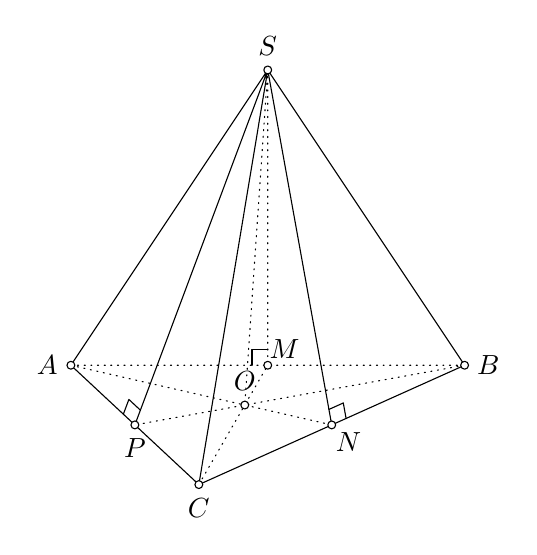
\begin{tikzpicture}[join=round,cap=round]
			\def\a{2.5}
			\pgfmathsetmacro\b{\a *cos(60) + .5}
			\path
			(180:\a) coordinate (A)
			(-120:\b) coordinate (C)
			(0:\a) coordinate (B)
			(90:1.5*\a) coordinate (S)
			($(A)!.5!(B)$) coordinate (M)
			($(B)!.5!(C)$) coordinate (N)
			($(C)!.5!(A)$) coordinate (P)
			(intersection of A--N and B--P) coordinate (O);
			\draw pic[draw,angle radius=2mm]{right angle = A--M--S};
			\draw pic[draw,angle radius=2mm]{right angle = B--N--S};
			\draw pic[draw,angle radius=2mm]{right angle = A--P--S};
			\draw[dotted] (A)--(B) (S)--(M) (A)--(N) (B)--(P) (C)--(M) (S)--(O);
			\draw (A)--(C)--(B)--(S)--cycle (S)--(C) (S)--(P) (S)--(N);
			\foreach \x in {} \draw[fill=white] (\x) circle (.05);
			\foreach \x/\g in {A/180,B/0,C/-90,S/90,M/45,N/-45,P/-90,O/90} \draw[fill=white] (\x) circle (.05) + (\g:.3) node{$\x$};
		\end{tikzpicture}
	\end{center}
	% TRIANGLE QUADRILATERAL
	\item {\it Problem: Triangles \& Quadrilaterals -- Bài Tập: Tam Giác \& Tứ Giác}.
	
	Folder: {\sf Elementary STEM \& Beyond{\tt/}Elementary Mathematics{\tt/}grade 8{\tt/}triangle quadrilateral{\tt/}problem}: [\href{https://github.com/NQBH/elementary_STEM_beyond/blob/main/elementary_mathematics/grade_8/triangle_quadrilateral/problem/NQBH_triangle_quadrilateral_problem.pdf}{pdf}\footnote{{\sc url}: \url{https://github.com/NQBH/elementary_STEM_beyond/blob/main/elementary_mathematics/grade_8/triangle_quadrilateral/problem/NQBH_triangle_quadrilateral_problem.pdf}.}][\href{https://github.com/NQBH/elementary_STEM_beyond/blob/main/elementary_mathematics/grade_8/triangle_quadrilateral/problem/NQBH_triangle_quadrilateral_problem.tex}{\TeX}\footnote{{\sc url}: \url{https://github.com/NQBH/elementary_STEM_beyond/blob/main/elementary_mathematics/grade_8/triangle_quadrilateral/problem/NQBH_triangle_quadrilateral_problem.tex}.}].
	\begin{itemize}
		\item {\it Problem \& Solution: Triangles \& Quadrilaterals -- Bài Tập \& Lời Giải: Tam Giác \& Tứ Giác}.
		
		Folder: {\sf Elementary STEM \& Beyond{\tt/}Elementary Mathematics{\tt/}grade 8{\tt/}triangle quadrilateral{\tt/}solution}: [\href{https://github.com/NQBH/elementary_STEM_beyond/blob/main/elementary_mathematics/grade_8/triangle_quadrilateral/solution/NQBH_triangle_quadrilateral_solution.pdf}{pdf}\footnote{{\sc url}: \url{https://github.com/NQBH/elementary_STEM_beyond/blob/main/elementary_mathematics/grade_8/triangle_quadrilateral/solution/NQBH_triangle_quadrilateral_solution.pdf}.}][\href{https://github.com/NQBH/elementary_STEM_beyond/blob/main/elementary_mathematics/grade_8/triangle_quadrilateral/solution/NQBH_triangle_quadrilateral_solution.tex}{\TeX}\footnote{{\sc url}: \url{https://github.com/NQBH/elementary_STEM_beyond/blob/main/elementary_mathematics/grade_8/triangle_quadrilateral/solution/NQBH_triangle_quadrilateral_solution.tex}.}].
	\end{itemize}
	% PROB STAT
	\item {\it Problem: Probability \& Statistics -- Bài Tập: Xác Suất \& Thống Kê}.
	
	Folder: {\sf Elementary STEM \& Beyond{\tt/}Elementary Mathematics{\tt/}grade 8{\tt/}probability \& statistics{\tt/}problem}: [\href{https://github.com/NQBH/elementary_STEM_beyond/blob/main/elementary_mathematics/grade_8/probability_statistics/problem/NQBH_probability_statistics_problem.pdf}{pdf}\footnote{{\sc url}: \url{https://github.com/NQBH/elementary_STEM_beyond/blob/main/elementary_mathematics/grade_8/probability_statistics/problem/NQBH_probability_statistics_problem.pdf}.}][\href{https://github.com/NQBH/elementary_STEM_beyond/blob/main/elementary_mathematics/grade_8/probability_statistics/problem/NQBH_probability_statistics_problem.tex}{\TeX}\footnote{{\sc url}: \url{https://github.com/NQBH/elementary_STEM_beyond/blob/main/elementary_mathematics/grade_8/probability_statistics/problem/NQBH_probability_statistics_problem.tex}.}].
	\begin{itemize}
		\item {\it Problem \& Solution: Probability \& Statistics -- Bài Tập \& Lời Giải: Xác Suất \& Thống Kê}.
		
		Folder: {\sf Elementary STEM \& Beyond{\tt/}Elementary Mathematics{\tt/}grade 8{\tt/}probability \& statistics{\tt/}solution}: [\href{https://github.com/NQBH/elementary_STEM_beyond/blob/main/elementary_mathematics/grade_8/probability_statistics/solution/NQBH_probability_statistics_solution.pdf}{pdf}\footnote{{\sc url}: \url{https://github.com/NQBH/elementary_STEM_beyond/blob/main/elementary_mathematics/grade_8/probability_statistics/solution/NQBH_probability_statistics_solution.pdf}.}][\href{https://github.com/NQBH/elementary_STEM_beyond/blob/main/elementary_mathematics/grade_8/probability_statistics/solution/NQBH_probability_statistics_solution.tex}{\TeX}\footnote{{\sc url}: \url{https://github.com/NQBH/elementary_STEM_beyond/blob/main/elementary_mathematics/grade_8/probability_statistics/solution/NQBH_probability_statistics_solution.tex}.}].
	\end{itemize}
	% LINEAR EQN
	\item {\it Problem: 1st-Order Polynomial Equation with 1 Variable $ax + b = 0$ -- Bài Tập: Phương Trình Bậc Nhất 1 Ẩn $ax + b = 0$}.
	
	Folder: {\sf Elementary STEM \& Beyond{\tt/}Elementary Mathematics{\tt/}grade 8{\tt/}1st-order polynomial equation 1 variable{\tt/}problem}: [\href{https://github.com/NQBH/elementary_STEM_beyond/blob/main/elementary_mathematics/grade_8/1st_order_polynomial_equation_1_variable/problem/NQBH_1st_order_polynomial_equation_1_variable_problem.pdf}{pdf}\footnote{{\sc url}: \url{https://github.com/NQBH/elementary_STEM_beyond/blob/main/elementary_mathematics/grade_8/1st_order_polynomial_equation_1_variable/problem/NQBH_1st_order_polynomial_equation_1_variable_problem.pdf}.}][\href{https://github.com/NQBH/elementary_STEM_beyond/blob/main/elementary_mathematics/grade_8/1st_order_polynomial_equation_1_variable/problem/NQBH_1st_order_polynomial_equation_1_variable_problem.tex}{\TeX}\footnote{{\sc url}: \url{https://github.com/NQBH/elementary_STEM_beyond/blob/main/elementary_mathematics/grade_8/1st_order_polynomial_equation_1_variable/problem/NQBH_1st_order_polynomial_equation_1_variable_problem.tex}.}].
	\begin{itemize}
		\item {\it Problem \& Solution: 1st-Order Polynomial Equation with 1 Variable $ax + b = 0$ -- Bài Tập \& Lời Giải: Phương Trình Bậc Nhất 1 Ẩn $ax + b = 0$}.
		
		Folder: {\sf Elementary STEM \& Beyond{\tt/}Elementary Mathematics{\tt/}grade 8{\tt/}1st-order polynomial equation 1 variable{\tt/}solution}: [\href{https://github.com/NQBH/elementary_STEM_beyond/blob/main/elementary_mathematics/grade_8/1st_order_polynomial_equation_1_variable/solution /NQBH_1st_order_polynomial_equation_1_variable_solution.pdf}{pdf}\footnote{{\sc url}: \url{https://github.com/NQBH/elementary_STEM_beyond/blob/main/elementary_mathematics/grade_8/1st_order_polynomial_equation_1_variable/solution /NQBH_1st_order_polynomial_equation_1_variable_solution.pdf}.}][\href{https://github.com/NQBH/elementary_STEM_beyond/blob/main/elementary_mathematics/grade_8/1st_order_polynomial_equation_1_variable/solution /NQBH_1st_order_polynomial_equation_1_variable_solution.tex}{\TeX}\footnote{{\sc url}: \url{https://github.com/NQBH/elementary_STEM_beyond/blob/main/elementary_mathematics/grade_8/1st_order_polynomial_equation_1_variable/solution /NQBH_1st_order_polynomial_equation_1_variable_solution.tex}.}].
	\end{itemize}
	% SIMILAR TRIANGLE
	\item {\it Problem: Similar Triangles \& Similar Shapes -- Bài Tập: Tam Giác Đồng Dạng \& Hình Đồng Dạng}.
	
	Folder: {\sf Elementary STEM \& Beyond{\tt/}Elementary Mathematics{\tt/}grade 8{\tt/}similar triangle{\tt/}problem}: [\href{https://github.com/NQBH/elementary_STEM_beyond/blob/main/elementary_mathematics/grade_8/similar_triangle/problem/NQBH_similar_triangle_problem.pdf}{pdf}\footnote{{\sc url}: \url{https://github.com/NQBH/elementary_STEM_beyond/blob/main/elementary_mathematics/grade_8/similar_triangle/problem/NQBH_similar_triangle_problem.pdf}.}][\href{https://github.com/NQBH/elementary_STEM_beyond/blob/main/elementary_mathematics/grade_8/similar_triangle/problem/NQBH_similar_triangle_problem.tex}{\TeX}\footnote{{\sc url}: \url{https://github.com/NQBH/elementary_STEM_beyond/blob/main/elementary_mathematics/grade_8/similar_triangle/problem/NQBH_similar_triangle_problem.tex}.}].
	\begin{itemize}
		\item {\it Problem \& Solution: Similar Triangles \& Similar Shapes -- Bài Tập \& Lời Giải: Tam Giác Đồng Dạng \& Hình Đồng Dạng}.
		
		Folder: {\sf Elementary STEM \& Beyond{\tt/}Elementary Mathematics{\tt/}grade 8{\tt/}similar triangle{\tt/}solution}: [\href{https://github.com/NQBH/elementary_STEM_beyond/blob/main/elementary_mathematics/grade_8/similar_triangle/solution/NQBH_similar_triangle_solution.pdf}{pdf}\footnote{{\sc url}: \url{https://github.com/NQBH/elementary_STEM_beyond/blob/main/elementary_mathematics/grade_8/similar_triangle/solution/NQBH_similar_triangle_solution.pdf}.}][\href{https://github.com/NQBH/elementary_STEM_beyond/blob/main/elementary_mathematics/grade_8/similar_triangle/solution/NQBH_similar_triangle_solution.tex}{\TeX}\footnote{{\sc url}: \url{https://github.com/NQBH/elementary_STEM_beyond/blob/main/elementary_mathematics/grade_8/similar_triangle/solution/NQBH_similar_triangle_solution.tex}.}].
	\end{itemize}
\end{enumerate}

\paragraph{Elementary Mathematics Grade 9 -- Toán sơ cấp lớp 9}

\begin{enumerate}
	\item {\it Cheatsheet: Elementary Mathematics Grade 9}.
	
	Folder: {\sf Elementary STEM \& Beyond{\tt/}Elementary Mathematics{\tt/}grade 9{\tt/}cheatsheet}: [\href{https://github.com/NQBH/elementary_STEM_beyond/blob/main/elementary_mathematics/grade_9/cheatsheet/NQBH_cheatsheet_mathematics_grade_9.pdf}{pdf}\footnote{{\sc url}: \url{https://github.com/NQBH/elementary_STEM_beyond/blob/main/elementary_mathematics/grade_9/cheatsheet/NQBH_cheatsheet_mathematics_grade_9.pdf}.}][\href{https://github.com/NQBH/elementary_STEM_beyond/blob/main/elementary_mathematics/grade_9/cheatsheet/NQBH_cheatsheet_mathematics_grade_9.tex}{\TeX}\footnote{{\sc url}: \url{https://github.com/NQBH/elementary_STEM_beyond/blob/main/elementary_mathematics/grade_9/cheatsheet/NQBH_cheatsheet_mathematics_grade_9.tex}.}].
	% LINEAR SYSTEM 1ST-ORDER EQNS
	\item {\it Problem: System of 1st-Order Equations -- Bài Tập: Hệ Phương Trình Bậc Nhất $A{\bf x} = {\bf b}$}.
	
	Folder: {\sf Elementary STEM \& Beyond{\tt/}Elementary Mathematics{\tt/}grade 9{\tt/}system of 1st-order equations{\tt/}problem}: [\href{https://github.com/NQBH/elementary_STEM_beyond/blob/main/elementary_mathematics/grade_9/system_1st_order_equations/problem/NQBH_system_1st_order_equations_problem.pdf}{pdf}\footnote{{\sc url}: \url{https://github.com/NQBH/elementary_STEM_beyond/blob/main/elementary_mathematics/grade_9/system_1st_order_equations/problem/NQBH_system_1st_order_equations_problem.pdf}.}][\href{https://github.com/NQBH/elementary_STEM_beyond/blob/main/elementary_mathematics/grade_9/system_1st_order_equations/problem/NQBH_system_1st_order_equations_problem.tex}{\TeX}\footnote{{\sc url}: \url{https://github.com/NQBH/elementary_STEM_beyond/blob/main/elementary_mathematics/grade_9/system_1st_order_equations/problem/NQBH_system_1st_order_equations_problem.tex}.}].
	\begin{itemize}
		\item {\it Problem \& Solution: System of 1st-Order Equations -- Bài Tập \& Lời Giải: Hệ Phương Trình Bậc Nhất $A{\bf x} = {\bf b}$}.
		
		Folder: {\sf Elementary STEM \& Beyond{\tt/}Elementary Mathematics{\tt/}grade 9{\tt/}system of 1st-order equations{\tt/}solution}: [\href{https://github.com/NQBH/elementary_STEM_beyond/blob/main/elementary_mathematics/grade_9/system_1st_order_equations/solution/NQBH_system_1st_order_equations_solution.pdf}{pdf}\footnote{{\sc url}: \url{https://github.com/NQBH/elementary_STEM_beyond/blob/main/elementary_mathematics/grade_9/system_1st_order_equations/solution/NQBH_system_1st_order_equations_solution.pdf}.}][\href{https://github.com/NQBH/elementary_STEM_beyond/blob/main/elementary_mathematics/grade_9/system_1st_order_equations/solution/NQBH_system_1st_order_equations_solution.tex}{\TeX}\footnote{{\sc url}: \url{https://github.com/NQBH/elementary_STEM_beyond/blob/main/elementary_mathematics/grade_9/system_1st_order_equations/solution/NQBH_system_1st_order_equations_solution.tex}.}].
	\end{itemize}
	% 1ST-ORDER INEQUATION
	\item {\it Problem: Inequality \& 1st-Order Inequation of 1 Unknown -- Bài Tập: Bất Đẳng Thức \& Bất Phương Trình Bậc Nhất 1 Ẩn}.
	
	Folder: {\sf Elementary STEM \& Beyond{\tt/}Elementary Mathematics{\tt/}grade 9{\tt/}1st-order inequation{\tt/}problem}: [\href{https://github.com/NQBH/elementary_STEM_beyond/blob/main/elementary_mathematics/grade_9/1st_order_inequation/problem/NQBH_1st_order_inequation_problem.pdf}{pdf}\footnote{{\sc url}: \url{https://github.com/NQBH/elementary_STEM_beyond/blob/main/elementary_mathematics/grade_9/1st_order_inequation/problem/NQBH_1st_order_inequation_problem.pdf}.}][\href{https://github.com/NQBH/elementary_STEM_beyond/blob/main/elementary_mathematics/grade_9/1st_order_inequation/problem/NQBH_1st_order_inequation_problem.tex}{\TeX}\footnote{{\sc url}: \url{https://github.com/NQBH/elementary_STEM_beyond/blob/main/elementary_mathematics/grade_9/1st_order_inequation/problem/NQBH_1st_order_inequation_problem.tex}.}].
	\begin{itemize}
		\item {\it Problem \& Solution: Inequality \& 1st-Order Inequation of 1 Unknown -- Bài Tập \& Lời Giải: Bất Đẳng Thức \& Bất Phương Trình Bậc Nhất 1 Ẩn}.
		
		Folder: {\sf Elementary STEM \& Beyond{\tt/}Elementary Mathematics{\tt/}grade 9{\tt/}1st-order inequation{\tt/}solution}: [\href{https://github.com/NQBH/elementary_STEM_beyond/blob/main/elementary_mathematics/grade_9/1st_order_inequation/solution/NQBH_1st_order_inequation_solution.pdf}{pdf}\footnote{{\sc url}: \url{https://github.com/NQBH/elementary_STEM_beyond/blob/main/elementary_mathematics/grade_9/1st_order_inequation/solution/NQBH_1st_order_inequation_solution.pdf}.}][\href{https://github.com/NQBH/elementary_STEM_beyond/blob/main/elementary_mathematics/grade_9/1st_order_inequation/solution/NQBH_1st_order_inequation_solution.tex}{\TeX}\footnote{{\sc url}: \url{https://github.com/NQBH/elementary_STEM_beyond/blob/main/elementary_mathematics/grade_9/1st_order_inequation/solution/NQBH_1st_order_inequation_solution.tex}.}].
	\end{itemize}
	% ROOT
	\item {\it Problem: Root $\sqrt{f(x)},\sqrt[3]{f(x)},\sqrt[n]{f(x)}$ -- Bài Tập: Căn Thức $\sqrt{f(x)},\sqrt[3]{f(x)},\sqrt[n]{f(x)}$}.
	
	Folder: {\sf Elementary STEM \& Beyond{\tt/}Elementary Mathematics{\tt/}grade 9{\tt/}root{\tt/}problem}: [\href{https://github.com/NQBH/elementary_STEM_beyond/blob/main/elementary_mathematics/grade_9/root/problem/NQBH_root_problem.pdf}{pdf}\footnote{{\sc url}: \url{https://github.com/NQBH/elementary_STEM_beyond/blob/main/elementary_mathematics/grade_9/root/problem/NQBH_root_problem.pdf}.}][\href{https://github.com/NQBH/elementary_STEM_beyond/blob/main/elementary_mathematics/grade_9/root/problem/NQBH_root_problem.tex}{\TeX}\footnote{{\sc url}: \url{https://github.com/NQBH/elementary_STEM_beyond/blob/main/elementary_mathematics/grade_9/root/problem/NQBH_root_problem.tex}.}].
	\begin{itemize}
		\item {\it Problem \& Solution: Root $\sqrt{f(x)},\sqrt[3]{f(x)},\sqrt[n]{f(x)}$ -- Bài Tập \& Lời Giải: Căn Thức $\sqrt{f(x)},\sqrt[3]{f(x)}$, $\sqrt[n]{f(x)}$}.
		
		Folder: {\sf Elementary STEM \& Beyond{\tt/}Elementary Mathematics{\tt/}grade 9{\tt/}root{\tt/}solution}: [\href{https://github.com/NQBH/elementary_STEM_beyond/blob/main/elementary_mathematics/grade_9/root/solution/NQBH_root_solution.pdf}{pdf}\footnote{{\sc url}: \url{https://github.com/NQBH/elementary_STEM_beyond/blob/main/elementary_mathematics/grade_9/root/solution/NQBH_root_solution.pdf}.}][\href{https://github.com/NQBH/elementary_STEM_beyond/blob/main/elementary_mathematics/grade_9/root/solution/NQBH_root_solution.tex}{\TeX}\footnote{{\sc url}: \url{https://github.com/NQBH/elementary_STEM_beyond/blob/main/elementary_mathematics/grade_9/root/solution/NQBH_root_solution.tex}.}].
	\end{itemize}	
	% TRIGONOMETRY
	\item {\it Problem: Trigonometry in Triangles -- Bài Tập: Hệ Thức Lượng Trong Tam Giác $\sin\alpha,\cos\alpha$, $\tan\alpha,\cot\alpha$}.
	
	Folder: {\sf Elementary STEM \& Beyond{\tt/}Elementary Mathematics{\tt/}grade 9{\tt/}trigonometry triangle{\tt/}problem}: [\href{https://github.com/NQBH/elementary_STEM_beyond/blob/main/elementary_mathematics/grade_9/trigonometry/problem/NQBH_trigonometry_problem.pdf}{pdf}\footnote{{\sc url}: \url{https://github.com/NQBH/elementary_STEM_beyond/blob/main/elementary_mathematics/grade_9/trigonometry/problem/NQBH_trigonometry_problem.pdf}.}][\href{https://github.com/NQBH/elementary_STEM_beyond/blob/main/elementary_mathematics/grade_9/trigonometry/problem/NQBH_trigonometry_problem.tex}{\TeX}\footnote{{\sc url}: \url{https://github.com/NQBH/elementary_STEM_beyond/blob/main/elementary_mathematics/grade_9/trigonometry/problem/NQBH_trigonometry_problem.tex}.}].
	
	\begin{baitoan}[{\sf Program}: Trigonometry in right triangles]
		Cho $\Delta ABC$ vuông tại $A$. (a) {\rm(Tính độ dài cạnh, đường cao, hình chiếu trong tam giác vuông)} Cho trước 2 yếu tố trong $6 + 15 = 21$ yếu tố gồm 6 số $a,b,c,b',c',h$ \& $C_6^2 = 15$ tỷ số của chúng:
		\begin{equation*}
			\frac{a}{b},\frac{a}{c},\frac{a}{b'},\frac{a}{c'},\frac{a}{h},\frac{b}{c},\frac{b}{b'},\frac{b}{c'},\frac{b}{h},\frac{c}{b'},\frac{c}{c'},\frac{c}{h},\frac{b'}{c'},\frac{b'}{h},\frac{c'}{h}.
		\end{equation*}
		Tìm công thức của 4 số còn lại theo 2 số đã cho. (b) Cho trước 2 trong $14 + 91 = 105$ yếu tố gồm 14 số $a,b,c$, $b',c',h$, $m_a,m_b,m_c$, $d_a,d_b,d_c$, $p,S$, \& $C_{14}^2 = 91$ tỷ số của chúng, với $d_a,d_b,d_c$ lần lượt là 3 đường phân giác ứng với $BC,CA,AB$. Tính 12 số còn lại theo 2 số đã cho. Viết các chương trình {\sf Pascal, Python, C{\tt/}C++} để giải bài toán.
	\end{baitoan}
	
	\begin{itemize}
		\item {\it Problem \& Solution: Trigonometry in Triangles -- Bài Tập \& Lời Giải: Hệ Thức Lượng Trong Tam Giác $\sin\alpha,\cos\alpha,\tan\alpha,\cot\alpha$}.
		
		Folder: {\sf Elementary STEM \& Beyond{\tt/}Elementary Mathematics{\tt/}grade 9{\tt/}trigonometry triangle{\tt/}solution}: [\href{https://github.com/NQBH/elementary_STEM_beyond/blob/main/elementary_mathematics/grade_9/trigonometry/solution/NQBH_trigonometry_solution.pdf}{pdf}\footnote{{\sc url}: \url{https://github.com/NQBH/elementary_STEM_beyond/blob/main/elementary_mathematics/grade_9/trigonometry/solution/NQBH_trigonometry_solution.pdf}.}][\href{https://github.com/NQBH/elementary_STEM_beyond/blob/main/elementary_mathematics/grade_9/trigonometry/solution/NQBH_trigonometry_solution.tex}{\TeX}\footnote{{\sc url}: \url{https://github.com/NQBH/elementary_STEM_beyond/blob/main/elementary_mathematics/grade_9/trigonometry/solution/NQBH_trigonometry_solution.tex}.}].
	\end{itemize}
	% CIRCLE
	\item {\it Problem: Circle -- Bài Tập: Đường Tròn}.
	
	Folder: {\sf Elementary STEM \& Beyond{\tt/}Elementary Mathematics{\tt/}grade 9{\tt/}circle{\tt/}problem}: [\href{https://github.com/NQBH/elementary_STEM_beyond/blob/main/elementary_mathematics/grade_9/circle/problem/NQBH_circle_problem.pdf}{pdf}\footnote{{\sc url}: \url{https://github.com/NQBH/elementary_STEM_beyond/blob/main/elementary_mathematics/grade_9/circle/problem/NQBH_circle_problem.pdf}.}][\href{https://github.com/NQBH/elementary_STEM_beyond/blob/main/elementary_mathematics/grade_9/circle/problem/NQBH_circle_problem.tex}{\TeX}\footnote{{\sc url}: \url{https://github.com/NQBH/elementary_STEM_beyond/blob/main/elementary_mathematics/grade_9/circle/problem/NQBH_circle_problem.tex}.}].
	\begin{itemize}
		\item {\it Problem \& Solution: Circle -- Bài Tập \& Lời Giải: Đường Tròn}.
		
		Folder: {\sf Elementary STEM \& Beyond{\tt/}Elementary Mathematics{\tt/}grade 9{\tt/}circle{\tt/}solution}: [\href{https://github.com/NQBH/elementary_STEM_beyond/blob/main/elementary_mathematics/grade_9/circle/solution/NQBH_circle_solution.pdf}{pdf}\footnote{{\sc url}: \url{https://github.com/NQBH/elementary_STEM_beyond/blob/main/elementary_mathematics/grade_9/circle/solution/NQBH_circle_solution.pdf}.}][\href{https://github.com/NQBH/elementary_STEM_beyond/blob/main/elementary_mathematics/grade_9/circle/solution/NQBH_circle_solution.tex}{\TeX}\footnote{{\sc url}: \url{https://github.com/NQBH/elementary_STEM_beyond/blob/main/elementary_mathematics/grade_9/circle/solution/NQBH_circle_solution.tex}.}].
	\end{itemize}
	% PROB STAT
	\item {\it Problem: Probability \& Statistics -- Bài Tập: Xác Suất \& Thống Kê}.
	
	Folder: {\sf Elementary STEM \& Beyond{\tt/}Elementary Mathematics{\tt/}grade 9{\tt/}probability \& statistics{\tt/}problem}: [\href{https://github.com/NQBH/elementary_STEM_beyond/blob/main/elementary_mathematics/grade_9/probability_statistics/problem/NQBH_probability_statistics_problem.pdf}{pdf}\footnote{{\sc url}: \url{https://github.com/NQBH/elementary_STEM_beyond/blob/main/elementary_mathematics/grade_9/probability_statistics/problem/NQBH_probability_statistics_problem.pdf}.}][\href{https://github.com/NQBH/elementary_STEM_beyond/blob/main/elementary_mathematics/grade_9/probability_statistics/problem/NQBH_probability_statistics_problem.tex}{\TeX}\footnote{{\sc url}: \url{https://github.com/NQBH/elementary_STEM_beyond/blob/main/elementary_mathematics/grade_9/probability_statistics/problem/NQBH_probability_statistics_problem.tex}.}].
	\begin{itemize}
		\item {\it Problem \& Solution: Probability \& Statistics -- Bài Tập \& Lời Giải: Xác Suất \& Thống Kê}.
		
		Folder: {\sf Elementary STEM \& Beyond{\tt/}Elementary Mathematics{\tt/}grade 9{\tt/}probability \& statistics{\tt/}solution}: [\href{https://github.com/NQBH/elementary_STEM_beyond/blob/main/elementary_mathematics/grade_9/probability_statistics/solution/NQBH_probability_statistics_solution.pdf}{pdf}\footnote{{\sc url}: \url{https://github.com/NQBH/elementary_STEM_beyond/blob/main/elementary_mathematics/grade_9/probability_statistics/solution/NQBH_probability_statistics_solution.pdf}.}][\href{https://github.com/NQBH/elementary_STEM_beyond/blob/main/elementary_mathematics/grade_9/probability_statistics/solution/NQBH_probability_statistics_solution.tex}{\TeX}\footnote{{\sc url}: \url{https://github.com/NQBH/elementary_STEM_beyond/blob/main/elementary_mathematics/grade_9/probability_statistics/solution/NQBH_probability_statistics_solution.tex}.}].
	\end{itemize}
	% QUADRATIC EQN	
	\item {\it Problem: 2nd-Order Function. Quadratic Equation -- Bài Tập: Hàm Số Bậc 2 $y = ax^2$. Phương Trình Bậc 2 1 Ẩn $ax^2 + bx + c = 0$}.
	
	Folder: {\sf Elementary STEM \& Beyond{\tt/}Elementary Mathematics{\tt/}grade 9{\tt/}2nd-order function, quadratic equation{\tt/}problem}: [\href{https://github.com/NQBH/elementary_STEM_beyond/blob/main/elementary_mathematics/grade_9/2nd_order_function/problem/NQBH_2nd_order_function_problem.pdf}{pdf}\footnote{{\sc url}: \url{https://github.com/NQBH/elementary_STEM_beyond/blob/main/elementary_mathematics/grade_9/2nd_order_function/problem/NQBH_2nd_order_function_problem.pdf}.}][\href{https://github.com/NQBH/elementary_STEM_beyond/blob/main/elementary_mathematics/grade_9/2nd_order_function/problem/NQBH_2nd_order_function_problem.tex}{\TeX}\footnote{{\sc url}: \url{https://github.com/NQBH/elementary_STEM_beyond/blob/main/elementary_mathematics/grade_9/2nd_order_function/problem/NQBH_2nd_order_function_problem.tex}.}].
	\begin{itemize}
		\item {\it Problem \& Solution: 2nd-Order Function. Quadratic Equation -- Bài Tập \& Lời Giải: Hàm Số Bậc 2 $y = ax^2$. Phương Trình Bậc 2 1 Ẩn $ax^2 + bx + c = 0$}.
		
		Folder: {\sf Elementary STEM \& Beyond{\tt/}Elementary Mathematics{\tt/}grade 9{\tt/}2nd-order function, quadratic equation{\tt/}solution}: [\href{https://github.com/NQBH/elementary_STEM_beyond/blob/main/elementary_mathematics/grade_9/2nd_order_function/solution/NQBH_2nd_order_function_solution.pdf}{pdf}\footnote{{\sc url}: \url{https://github.com/NQBH/elementary_STEM_beyond/blob/main/elementary_mathematics/grade_9/2nd_order_function/solution/NQBH_2nd_order_function_solution.pdf}.}][\href{https://github.com/NQBH/elementary_STEM_beyond/blob/main/elementary_mathematics/grade_9/2nd_order_function/solution/NQBH_2nd_order_function_solution.tex}{\TeX}\footnote{{\sc url}: \url{https://github.com/NQBH/elementary_STEM_beyond/blob/main/elementary_mathematics/grade_9/2nd_order_function/solution/NQBH_2nd_order_function_solution.tex}.}].
	\end{itemize}
	% CIRCUMCIRCLE INCIRCLE	
	\item {\it Problem: Circumcircle {\it\&} Incircle -- Bài Tập: Đường Tròn Ngoại Tiếp {\it\&} Đường Tròn Nội Tiếp}.
	
	Folder: {\sf Elementary STEM \& Beyond{\tt/}Elementary Mathematics{\tt/}grade 9{\tt/}circumcircle \& incircle{\tt/}problem}: [\href{https://github.com/NQBH/elementary_STEM_beyond/blob/main/elementary_mathematics/grade_9/circumcircle_incircle/problem/NQBH_circumcircle_incircle_problem.pdf}{pdf}\footnote{{\sc url}: \url{https://github.com/NQBH/elementary_STEM_beyond/blob/main/elementary_mathematics/grade_9/circumcircle_incircle/problem/NQBH_circumcircle_incircle_problem.pdf}.}][\href{https://github.com/NQBH/elementary_STEM_beyond/blob/main/elementary_mathematics/grade_9/circumcircle_incircle/problem/NQBH_circumcircle_incircle_problem.tex}{\TeX}\footnote{{\sc url}: \url{https://github.com/NQBH/elementary_STEM_beyond/blob/main/elementary_mathematics/grade_9/circumcircle_incircle/problem/NQBH_circumcircle_incircle_problem.tex}.}].
	\begin{itemize}
		\item {\it Problem \& Solution: Circumcircle \& Incircle -- Bài Tập \& Lời Giải: Đường Tròn Ngoại Tiếp \& Đường Tròn Nội Tiếp}.
		
		Folder: {\sf Elementary STEM \& Beyond{\tt/}Elementary Mathematics{\tt/}grade 9{\tt/}circumcircle \& incircle{\tt/}solution}: [\href{https://github.com/NQBH/elementary_STEM_beyond/blob/main/elementary_mathematics/grade_9/circumcircle_incircle/solution/NQBH_circumcircle_incircle_solution.pdf}{pdf}\footnote{{\sc url}: \url{https://github.com/NQBH/elementary_STEM_beyond/blob/main/elementary_mathematics/grade_9/circumcircle_incircle/solution/NQBH_circumcircle_incircle_solution.pdf}.}][\href{https://github.com/NQBH/elementary_STEM_beyond/blob/main/elementary_mathematics/grade_9/circumcircle_incircle/solution/NQBH_circumcircle_incircle_solution.tex}{\TeX}\footnote{{\sc url}: \url{https://github.com/NQBH/elementary_STEM_beyond/blob/main/elementary_mathematics/grade_9/circumcircle_incircle/solution/NQBH_circumcircle_incircle_solution.tex}.}].
	\end{itemize}
	% REGULAR POLYGONS
	\item {\it Problem: Regular Polygons -- Bài Tập: Đa Giác Đều}.
	
	Folder: {\sf Elementary STEM \& Beyond{\tt/}Elementary Mathematics{\tt/}grade 9{\tt/}regular polygon{\tt/}problem}: [\href{https://github.com/NQBH/elementary_STEM_beyond/blob/main/elementary_mathematics/grade_9/regular_polygon/problem/NQBH_regular_polygon_problem.pdf}{pdf}\footnote{{\sc url}: \url{https://github.com/NQBH/elementary_STEM_beyond/blob/main/elementary_mathematics/grade_9/regular_polygon/problem/NQBH_regular_polygon_problem.pdf}.}][\href{https://github.com/NQBH/elementary_STEM_beyond/blob/main/elementary_mathematics/grade_9/regular_polygon/problem/NQBH_regular_polygon_problem.tex}{\TeX}\footnote{{\sc url}: \url{https://github.com/NQBH/elementary_STEM_beyond/blob/main/elementary_mathematics/grade_9/regular_polygon/problem/NQBH_regular_polygon_problem.tex}.}].
	\begin{itemize}
		\item {\it Problem \& Solution: Regular Polygons -- Bài Tập \& Lời Giải: Đa Giác Đều}.
		
		Folder: {\sf Elementary STEM \& Beyond{\tt/}Elementary Mathematics{\tt/}grade 9{\tt/}regular polygon{\tt/}solution}: [\href{https://github.com/NQBH/elementary_STEM_beyond/blob/main/elementary_mathematics/grade_9/regular_polygon/solution/NQBH_regular_polygon_solution.pdf}{pdf}\footnote{{\sc url}: \url{https://github.com/NQBH/elementary_STEM_beyond/blob/main/elementary_mathematics/grade_9/regular_polygon/solution/NQBH_regular_polygon_solution.pdf}.}][\href{https://github.com/NQBH/elementary_STEM_beyond/blob/main/elementary_mathematics/grade_9/regular_polygon/solution/NQBH_regular_polygon_solution.tex}{\TeX}\footnote{{\sc url}: \url{https://github.com/NQBH/elementary_STEM_beyond/blob/main/elementary_mathematics/grade_9/regular_polygon/solution/NQBH_regular_polygon_solution.tex}.}].
	\end{itemize}
	% CYLINDER CONE SPHERE	
	\item {\it Problem: Cylinder, Cone, Sphere -- Bài Tập: Hình Trụ, Hình Nón, Hình Cầu}.
	\begin{center}
		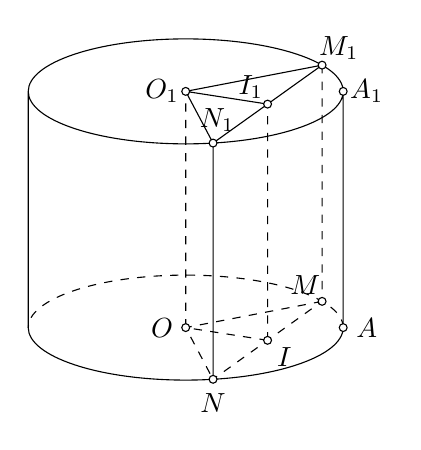
\begin{tikzpicture}
			\def\r{2}
			\def\h{3}
			\def\gM{30}
			\def\gN{-80}
			\path
			(0:0) coordinate (O)
			(0:\r) coordinate (A)
			(180:\r) coordinate (B)
			(A) arc (0:\gM:{\r} and {\r/3}) coordinate (M)
			(A) arc (0:\gN:{\r} and {\r/3}) coordinate (N)
			($(M)!.5!(N)$) coordinate (I)
			\foreach \x in {O,A,B,M,N,I}{(\x)++(90:\h) coordinate (\x_1)};
			\draw[dashed]
			(I)--(O)--(O_1) (M)--(O)--(N) (M_1)--(M)--(N) (I)--(I_1) (A) arc (0:180:{\r} and {\r/3});
			\draw (A) arc (0:-180:{\r} and {\r/3}) (O_1) ellipse ({\r} and {\r/3}) (A)--(A_1) (B)--(B_1) (N)--(N_1) (O_1)--(I_1) (O_1)--(M_1)--(N_1)--cycle;
			\foreach \x/\g in {A/0,A_1/0,O/180,O_1/180,I/-45,M/135,N/-90,M_1/45,N_1/80,I_1/135} \draw[fill=white] (\x) circle (.05) + (\g:.3) node{$\x$};
		\end{tikzpicture}
		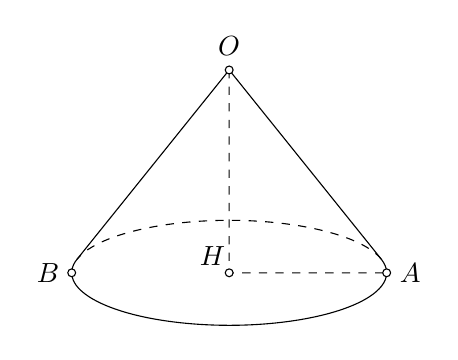
\begin{tikzpicture}
			\def\r{2}
			\def\gM{15}
			\path
			(0:0) coordinate (H)
			(0:\r) coordinate (A)
			(180:\r) coordinate (B)
			(A) arc (0:\gM:{\r} and {\r/3}) coordinate (M)--([turn]0:1mm) coordinate (Mt)
			(B) arc (180:180-\gM:{\r} and {\r/3}) coordinate (M')--([turn]0:1mm) coordinate (M't)
			(intersection of M--Mt and M'--M't) coordinate (O);
			\draw[dashed] (O)--(H)--(A) (M) arc (\gM:180-\gM:{\r} and {\r/3});
			\draw (M') arc (180-\gM:360+\gM:{\r} and {\r/3}) (M)--(O)--(M');
			\foreach \x/\g in {A/0,B/180,O/90,H/135} \draw[fill=white] (\x) circle (.05) + (\g:.3) node{$\x$};
		\end{tikzpicture}
		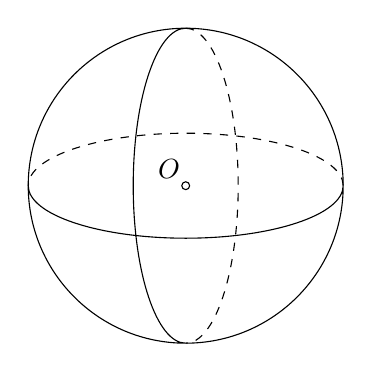
\begin{tikzpicture}
			\def\r{2}
			\path (0:0) coordinate (O);
			\draw[dashed] (0:\r) arc (0:180:{\r} and {\r/3}) (90:\r) arc (90:-90:{\r/3} and {\r});
			\draw (O) circle (\r) (180:\r) arc (180:360:{\r} and {\r/3}) (90:\r) arc (90:270:{\r/3} and {\r});
			\foreach \x/\g in {O/135} \draw[fill=white] (\x) circle (.05) + (\g:.3) node{$\x$};
		\end{tikzpicture}
	\end{center}
	Folder: {\sf Elementary STEM \& Beyond{\tt/}Elementary Mathematics{\tt/}grade 9{\tt/}cylinder, cone, sphere{\tt/}problem}: [\href{https://github.com/NQBH/elementary_STEM_beyond/blob/main/elementary_mathematics/grade_9/cylinder_cone_sphere/problem/NQBH_cylinder_cone_sphere_problem.pdf}{pdf}\footnote{{\sc url}: \url{https://github.com/NQBH/elementary_STEM_beyond/blob/main/elementary_mathematics/grade_9/cylinder_cone_sphere/problem/NQBH_cylinder_cone_sphere_problem.pdf}.}][\href{https://github.com/NQBH/elementary_STEM_beyond/blob/main/elementary_mathematics/grade_9/cylinder_cone_sphere/problem/NQBH_cylinder_cone_sphere_problem.tex}{\TeX}\footnote{{\sc url}: \url{https://github.com/NQBH/elementary_STEM_beyond/blob/main/elementary_mathematics/grade_9/cylinder_cone_sphere/problem/NQBH_cylinder_cone_sphere_problem.tex}.}].
	\begin{itemize}
		\item  {\it Problem \& Solution: Cylinder, Cone, Sphere -- Bài Tập \& Lời Giải: Hình Trụ, Hình Nón, Hình Cầu}.
		
		Folder: {\sf Elementary STEM \& Beyond{\tt/}Elementary Mathematics{\tt/}grade 9{\tt/}cylinder, cone, sphere{\tt/}solution}: [\href{https://github.com/NQBH/elementary_STEM_beyond/blob/main/elementary_mathematics/grade_9/cylinder_cone_sphere/solution/NQBH_cylinder_cone_sphere_solution.pdf}{pdf}\footnote{{\sc url}: \url{https://github.com/NQBH/elementary_STEM_beyond/blob/main/elementary_mathematics/grade_9/cylinder_cone_sphere/solution/NQBH_cylinder_cone_sphere_solution.pdf}.}][\href{https://github.com/NQBH/elementary_STEM_beyond/blob/main/elementary_mathematics/grade_9/cylinder_cone_sphere/solution/NQBH_cylinder_cone_sphere_solution.tex}{\TeX}\footnote{{\sc url}: \url{https://github.com/NQBH/elementary_STEM_beyond/blob/main/elementary_mathematics/grade_9/cylinder_cone_sphere/solution/NQBH_cylinder_cone_sphere_solution.tex}.}].
	\end{itemize}
\end{enumerate}

\paragraph{Elementary Mathematics Grade 10 -- Toán sơ cấp lớp 10}

\begin{enumerate}
	\item {\it Cheatsheet: Elementary Mathematics Grade 10}.
	
	Folder: {\sf Elementary STEM \& Beyond{\tt/}Elementary Mathematics{\tt/}grade 10{\tt/}cheatsheet}: [\href{.pdf}{pdf}\footnote{{\sc url}: \url{.pdf}.}][\href{.tex}{\TeX}\footnote{{\sc url}: \url{.tex}.}].
	% PROP SET
	\item {\it Problem: Proposition \& Set -- Bài Tập: Mệnh Đề \& Tập Hợp}.
	
	Folder: {\sf Elementary STEM \& Beyond{\tt/}Elementary Mathematics{\tt/}grade 10{\tt/}proposition \& set{\tt/}problem}: [\href{https://github.com/NQBH/elementary_STEM_beyond/blob/main/elementary_mathematics/grade_10/proposition_set/problem/NQBH_proposition_set_problem.pdf}{pdf}\footnote{{\sc url}: \url{https://github.com/NQBH/elementary_STEM_beyond/blob/main/elementary_mathematics/grade_10/proposition_set/problem/NQBH_proposition_set_problem.pdf}.}][\href{https://github.com/NQBH/elementary_STEM_beyond/blob/main/elementary_mathematics/grade_10/proposition_set/problem/NQBH_proposition_set_problem.tex}{\TeX}\footnote{{\sc url}: \url{https://github.com/NQBH/elementary_STEM_beyond/blob/main/elementary_mathematics/grade_10/proposition_set/problem/NQBH_proposition_set_problem.tex}.}].
	\begin{itemize}
		\item {\it Problem \& Solution: Proposition \& Set -- Bài Tập \& Lời Giải: Mệnh Đề \& Tập Hợp}.
		
		Folder: {\sf Elementary STEM \& Beyond{\tt/}Elementary Mathematics{\tt/}grade 10{\tt/}proposition \& set{\tt/}solution}: [\href{https://github.com/NQBH/elementary_STEM_beyond/blob/main/elementary_mathematics/grade_10/proposition_set/solution/NQBH_proposition_set_solution.pdf}{pdf}\footnote{{\sc url}: \url{https://github.com/NQBH/elementary_STEM_beyond/blob/main/elementary_mathematics/grade_10/proposition_set/solution/NQBH_proposition_set_solution.pdf}.}][\href{https://github.com/NQBH/elementary_STEM_beyond/blob/main/elementary_mathematics/grade_10/proposition_set/solution/NQBH_proposition_set_solution.tex}{\TeX}\footnote{{\sc url}: \url{https://github.com/NQBH/elementary_STEM_beyond/blob/main/elementary_mathematics/grade_10/proposition_set/solution/NQBH_proposition_set_solution.tex}.}].
	\end{itemize}
	% LINEAR SYS INEQNS
	\item {\it Problem: Inequation \& Linear System of Inequations -- Bài Tập: Bất Phương Trình \& Hệ Bất Phương Trình}.
	
	Folder: {\sf Elementary STEM \& Beyond{\tt/}Elementary Mathematics{\tt/}grade 10{\tt/}linear system inequations{\tt/}problem}: [\href{https://github.com/NQBH/elementary_STEM_beyond/blob/main/elementary_mathematics/grade_10/linear_system_inequations/problem/NQBH_linear_system_inequations_problem.pdf}{pdf}\footnote{{\sc url}: \url{https://github.com/NQBH/elementary_STEM_beyond/blob/main/elementary_mathematics/grade_10/linear_system_inequations/problem/NQBH_linear_system_inequations_problem.pdf}.}][\href{https://github.com/NQBH/elementary_STEM_beyond/blob/main/elementary_mathematics/grade_10/linear_system_inequations/problem/NQBH_linear_system_inequations_problem.tex}{\TeX}\footnote{{\sc url}: \url{https://github.com/NQBH/elementary_STEM_beyond/blob/main/elementary_mathematics/grade_10/linear_system_inequations/problem/NQBH_linear_system_inequations_problem.tex}.}].
	\begin{itemize}
		\item {\it Problem \& Solution: Inequation \& Linear System of Inequations -- Bài Tập \& Lời Giải: Bất Phương Trình \& Hệ Bất Phương Trình}.
		
		Folder: {\sf Elementary STEM \& Beyond{\tt/}Elementary Mathematics{\tt/}grade 10{\tt/}linear system inequations{\tt/}solution}: [\href{https://github.com/NQBH/elementary_STEM_beyond/blob/main/elementary_mathematics/grade_10/linear_system_inequations/solution/NQBH_linear_system_inequations_solution.pdf}{pdf}\footnote{{\sc url}: \url{https://github.com/NQBH/elementary_STEM_beyond/blob/main/elementary_mathematics/grade_10/linear_system_inequations/solution/NQBH_linear_system_inequations_solution.pdf}.}][\href{https://github.com/NQBH/elementary_STEM_beyond/blob/main/elementary_mathematics/grade_10/linear_system_inequations/solution/NQBH_linear_system_inequations_solution.tex}{\TeX}\footnote{{\sc url}: \url{https://github.com/NQBH/elementary_STEM_beyond/blob/main/elementary_mathematics/grade_10/linear_system_inequations/solution/NQBH_linear_system_inequations_solution.tex}.}].
	\end{itemize}
	% FUNC GRAPH
	\item {\it Problem: Function \& Graph  -- Bài Tập: Hàm Số \& Đồ Thị}.
	
	Folder: {\sf Elementary STEM \& Beyond{\tt/}Elementary Mathematics{\tt/}grade 10{\tt/}function graph{\tt/}problem}: [\href{https://github.com/NQBH/elementary_STEM_beyond/blob/main/elementary_mathematics/grade_10/function_graph/problem/NQBH_function_graph_problem.pdf}{pdf}\footnote{{\sc url}: \url{https://github.com/NQBH/elementary_STEM_beyond/blob/main/elementary_mathematics/grade_10/function_graph/problem/NQBH_function_graph_problem.pdf}.}][\href{https://github.com/NQBH/elementary_STEM_beyond/blob/main/elementary_mathematics/grade_10/function_graph/problem/NQBH_function_graph_problem.tex}{\TeX}\footnote{{\sc url}: \url{https://github.com/NQBH/elementary_STEM_beyond/blob/main/elementary_mathematics/grade_10/function_graph/problem/NQBH_function_graph_problem.tex}.}].
	\begin{itemize}
		\item {\it Problem \& Solution: Function \& Graph  -- Bài Tập \& Lời Giải: Hàm Số \& Đồ Thị}.
		
		Folder: {\sf Elementary STEM \& Beyond{\tt/}Elementary Mathematics{\tt/}grade 10{\tt/}function graph{\tt/}solution}: [\href{https://github.com/NQBH/elementary_STEM_beyond/blob/main/elementary_mathematics/grade_10/function_graph/solution/NQBH_function_graph_solution.pdf}{pdf}\footnote{{\sc url}: \url{https://github.com/NQBH/elementary_STEM_beyond/blob/main/elementary_mathematics/grade_10/function_graph/solution/NQBH_function_graph_solution.pdf}.}][\href{https://github.com/NQBH/elementary_STEM_beyond/blob/main/elementary_mathematics/grade_10/function_graph/solution/NQBH_function_graph_solution.tex}{\TeX}\footnote{{\sc url}: \url{https://github.com/NQBH/elementary_STEM_beyond/blob/main/elementary_mathematics/grade_10/function_graph/solution/NQBH_function_graph_solution.tex}.}].
	\end{itemize}
	% TRIGONOMETRY
	\item {\it Problem: Trigonometrical Identities in Triangles -- Bài Tập: Hệ Thức Lượng Trong Tam Giác}.
	
	Folder: {\sf Elementary STEM \& Beyond{\tt/}Elementary Mathematics{\tt/}grade 10{\tt/}trigonometry{\tt/}problem}: [\href{https://github.com/NQBH/elementary_STEM_beyond/blob/main/elementary_mathematics/grade_10/trigonometry/problem/NQBH_trigonometry_problem.pdf}{pdf}\footnote{{\sc url}: \url{https://github.com/NQBH/elementary_STEM_beyond/blob/main/elementary_mathematics/grade_10/trigonometry/problem/NQBH_trigonometry_problem.pdf}.}][\href{https://github.com/NQBH/elementary_STEM_beyond/blob/main/elementary_mathematics/grade_10/trigonometry/problem/NQBH_trigonometry_problem.tex}{\TeX}\footnote{{\sc url}: \url{https://github.com/NQBH/elementary_STEM_beyond/blob/main/elementary_mathematics/grade_10/trigonometry/problem/NQBH_trigonometry_problem.tex}.}].
	\begin{itemize}
		\item {\it Problem \& Solution: Trigonometrical Identities in Triangles -- Bài Tập \& Lời Giải: Hệ Thức Lượng Trong Tam Giác}.
		
		Folder: {\sf Elementary STEM \& Beyond{\tt/}Elementary Mathematics{\tt/}grade 10{\tt/}trigonometry{\tt/}solution}: [\href{https://github.com/NQBH/elementary_STEM_beyond/blob/main/elementary_mathematics/grade_10/trigonometry/solution/NQBH_trigonometry_solution.pdf}{pdf}\footnote{{\sc url}: \url{https://github.com/NQBH/elementary_STEM_beyond/blob/main/elementary_mathematics/grade_10/trigonometry/solution/NQBH_trigonometry_solution.pdf}.}][\href{https://github.com/NQBH/elementary_STEM_beyond/blob/main/elementary_mathematics/grade_10/trigonometry/solution/NQBH_trigonometry_solution.tex}{\TeX}\footnote{{\sc url}: \url{https://github.com/NQBH/elementary_STEM_beyond/blob/main/elementary_mathematics/grade_10/trigonometry/solution/NQBH_trigonometry_solution.tex}.}].
	\end{itemize}
	{\it A bridge between Elementary Algebra \& Elementary Geometric $+$ Trigonometric -- Nhịp cầu nối giữa Đại Số Sơ Cấp với Hình Học Sơ Cấp \& Lượng giác}: Các yếu tố hình học \& lượng giác của tam giác, e.g., cạnh $a,b,c$, đường cao $h_a,h_b,h_c$, đường trung tuyến $m_a,m_b,m_c$, đường phân giác trong $l_a,l_b,l_c$, các bán kính đường tròn nội tiếp $r$, ngoại tiếp $R$, bàng tiếp $r_a,r_b,r_c,\ldots$ \& các tỷ số lượng giác $\sin,\cos,\tan,\cot,\ldots$ các góc $\angle A,\angle B,\angle C$ của tam giác, chính là các nghiệm của phương trình bậc 3 (3rd-degree polynomial equation or cubic equation) mà các hệ số phụ thuộc vào 3 yếu tố cơ bản $p,R,r$, lần lượt là nửa chu vi, bán kính đường tròn ngoại tiếp, nội tiếp của tam giác, see \cite{Phuong_Quan_ptb3_htl}.
	% VECTOR
	\item {\it Problem: Vector -- Bài Tập: Vector}.
	
	Folder: {\sf Elementary STEM \& Beyond{\tt/}Elementary Mathematics{\tt/}grade 10{\tt/}vector{\tt/}problem}: [\href{https://github.com/NQBH/elementary_STEM_beyond/blob/main/elementary_mathematics/grade_10/vector/problem/NQBH_vector_problem.pdf}{pdf}\footnote{{\sc url}: \url{https://github.com/NQBH/elementary_STEM_beyond/blob/main/elementary_mathematics/grade_10/vector/problem/NQBH_vector_problem.pdf}.}][\href{https://github.com/NQBH/elementary_STEM_beyond/blob/main/elementary_mathematics/grade_10/vector/problem/NQBH_vector_problem.tex}{\TeX}\footnote{{\sc url}: \url{https://github.com/NQBH/elementary_STEM_beyond/blob/main/elementary_mathematics/grade_10/vector/problem/NQBH_vector_problem.tex}.}].
	\begin{itemize}
		\item {\it Problem \& Solution: Vector -- Bài Tập \& Lời Giải: Vector}.
		
		Folder: {\sf Elementary STEM \& Beyond{\tt/}Elementary Mathematics{\tt/}grade 10{\tt/}vector{\tt/}solution}: [\href{https://github.com/NQBH/elementary_STEM_beyond/blob/main/elementary_mathematics/grade_10/vector/solution/NQBH_vector_solution.pdf}{pdf}\footnote{{\sc url}: \url{https://github.com/NQBH/elementary_STEM_beyond/blob/main/elementary_mathematics/grade_10/vector/solution/NQBH_vector_solution.pdf}.}][\href{https://github.com/NQBH/elementary_STEM_beyond/blob/main/elementary_mathematics/grade_10/vector/solution/NQBH_vector_solution.tex}{\TeX}\footnote{{\sc url}: \url{https://github.com/NQBH/elementary_STEM_beyond/blob/main/elementary_mathematics/grade_10/vector/solution/NQBH_vector_solution.tex}.}].
	\end{itemize}
	% COMBINATORICS
	\item {\it Problem: Combinatorics -- Bài Tập: Đại Số Tổ Hợp}.
	
	Folder: {\sf Elementary STEM \& Beyond{\tt/}Elementary Mathematics{\tt/}grade 10{\tt/}combinatorics{\tt/}problem}: [\href{https://github.com/NQBH/elementary_STEM_beyond/blob/main/elementary_mathematics/grade_10/combinatorics/problem/NQBH_combinatorics_problem.pdf}{pdf}\footnote{{\sc url}: \url{https://github.com/NQBH/elementary_STEM_beyond/blob/main/elementary_mathematics/grade_10/combinatorics/problem/NQBH_combinatorics_problem.pdf}.}][\href{https://github.com/NQBH/elementary_STEM_beyond/blob/main/elementary_mathematics/grade_10/combinatorics/problem/NQBH_combinatorics_problem.tex}{\TeX}\footnote{{\sc url}: \url{https://github.com/NQBH/elementary_STEM_beyond/blob/main/elementary_mathematics/grade_10/combinatorics/problem/NQBH_combinatorics_problem.tex}.}].
	\begin{itemize}
		\item {\it Problem \& Solution: Combinatorics -- Bài Tập \& Lời Giải: Đại Số Tổ Hợp}.
		
		Folder: {\sf Elementary STEM \& Beyond{\tt/}Elementary Mathematics{\tt/}grade 10{\tt/}combinatorics{\tt/}solution}: [\href{https://github.com/NQBH/elementary_STEM_beyond/blob/main/elementary_mathematics/grade_10/combinatorics/solution/NQBH_combinatorics_solution.pdf}{pdf}\footnote{{\sc url}: \url{https://github.com/NQBH/elementary_STEM_beyond/blob/main/elementary_mathematics/grade_10/combinatorics/solution/NQBH_combinatorics_solution.pdf}.}][\href{https://github.com/NQBH/elementary_STEM_beyond/blob/main/elementary_mathematics/grade_10/combinatorics/solution/NQBH_combinatorics_solution.tex}{\TeX}\footnote{{\sc url}: \url{https://github.com/NQBH/elementary_STEM_beyond/blob/main/elementary_mathematics/grade_10/combinatorics/solution/NQBH_combinatorics_solution.tex}.}].
	\end{itemize}
	% PROB & STAT
	\item {\it Problem: Probability \& Statistics -- Bài Tập: Xác Suất \& Thống Kê}.
	
	Folder: {\sf Elementary STEM \& Beyond{\tt/}Elementary Mathematics{\tt/}grade 10{\tt/}probability \& statistics{\tt/}problem}: [\href{https://github.com/NQBH/elementary_STEM_beyond/blob/main/elementary_mathematics/grade_10/probability_statistics/problem/NQBH_probability_statistics_problem.pdf}{pdf}\footnote{{\sc url}: \url{https://github.com/NQBH/elementary_STEM_beyond/blob/main/elementary_mathematics/grade_10/probability_statistics/problem/NQBH_probability_statistics_problem.pdf}.}][\href{https://github.com/NQBH/elementary_STEM_beyond/blob/main/elementary_mathematics/grade_10/probability_statistics/problem/NQBH_probability_statistics_problem.tex}{\TeX}\footnote{{\sc url}: \url{https://github.com/NQBH/elementary_STEM_beyond/blob/main/elementary_mathematics/grade_10/probability_statistics/problem/NQBH_probability_statistics_problem.tex}.}].
	\begin{itemize}
		\item {\it Problem \& Solution: Probability \& Statistics -- Bài Tập \& Lời Giải: Xác Suất \& Thống Kê}.
		
		Folder: {\sf Elementary STEM \& Beyond{\tt/}Elementary Mathematics{\tt/}grade 10{\tt/}probability \& statistics{\tt/}solution}: [\href{https://github.com/NQBH/elementary_STEM_beyond/blob/main/elementary_mathematics/grade_10/probability_statistics/solution/NQBH_probability_statistics_solution.pdf}{pdf}\footnote{{\sc url}: \url{https://github.com/NQBH/elementary_STEM_beyond/blob/main/elementary_mathematics/grade_10/probability_statistics/solution/NQBH_probability_statistics_solution.pdf}.}][\href{https://github.com/NQBH/elementary_STEM_beyond/blob/main/elementary_mathematics/grade_10/probability_statistics/solution/NQBH_probability_statistics_solution.tex}{\TeX}\footnote{{\sc url}: \url{https://github.com/NQBH/elementary_STEM_beyond/blob/main/elementary_mathematics/grade_10/probability_statistics/solution/NQBH_probability_statistics_solution.tex}.}].
	\end{itemize}
	% 2D COORDINATE
	\item {\it Problem: 2D Method of Cartesian Coordinates -- Bài Tập: Phương Pháp Tọa Độ Cartesian Trong Mặt Phẳng}.
	
	Folder: {\sf Elementary STEM \& Beyond{\tt/}Elementary Mathematics{\tt/}grade 10{\tt/}2D method of coordinate{\tt/}problem}: [\href{https://github.com/NQBH/elementary_STEM_beyond/blob/main/elementary_mathematics/grade_10/2D_method_coordinate/problem/NQBH_2D_method_coordinate_problem.pdf}{pdf}\footnote{{\sc url}: \url{https://github.com/NQBH/elementary_STEM_beyond/blob/main/elementary_mathematics/grade_10/2D_method_coordinate/problem/NQBH_2D_method_coordinate_problem.pdf}.}][\href{https://github.com/NQBH/elementary_STEM_beyond/blob/main/elementary_mathematics/grade_10/2D_method_coordinate/problem/NQBH_2D_method_coordinate_problem.tex}{\TeX}\footnote{{\sc url}: \url{https://github.com/NQBH/elementary_STEM_beyond/blob/main/elementary_mathematics/grade_10/2D_method_coordinate/problem/NQBH_2D_method_coordinate_problem.tex}.}].
	\begin{itemize}
		\item {\it Problem \& Solution: 2D Method of Cartesian Coordinates -- Bài Tập \& Lời Giải: Phương Pháp Tọa Độ Cartesian Trong Mặt Phẳng}.
		
		Folder: {\sf Elementary STEM \& Beyond{\tt/}Elementary Mathematics{\tt/}grade 10{\tt/}2D method of coordinate{\tt/}solution}: [\href{https://github.com/NQBH/elementary_STEM_beyond/blob/main/elementary_mathematics/grade_10/2D_method_coordinate/solution/NQBH_2D_method_coordinate_solution.pdf}{pdf}\footnote{{\sc url}: \url{https://github.com/NQBH/elementary_STEM_beyond/blob/main/elementary_mathematics/grade_10/2D_method_coordinate/solution/NQBH_2D_method_coordinate_solution.pdf}.}][\href{https://github.com/NQBH/elementary_STEM_beyond/blob/main/elementary_mathematics/grade_10/2D_method_coordinate/solution/NQBH_2D_method_coordinate_solution.tex}{\TeX}\footnote{{\sc url}: \url{https://github.com/NQBH/elementary_STEM_beyond/blob/main/elementary_mathematics/grade_10/2D_method_coordinate/solution/NQBH_2D_method_coordinate_solution.tex}.}].
	\end{itemize}
	% INDUCTION
	\item {\it Problem: Mathematical Induction \& Newton Binomial -- Bài Tập: Phương Pháp Quy Nạp Toán Học \& Nhị Thức Newton}.
	
	Folder: {\sf Elementary STEM \& Beyond{\tt/}Elementary Mathematics{\tt/}grade 10{\tt/}induction{\tt/}problem}: [\href{https://github.com/NQBH/elementary_STEM_beyond/blob/main/elementary_mathematics/grade_10/induction/problem/NQBH_mathematical_induction_problem.pdf}{pdf}\footnote{{\sc url}: \url{https://github.com/NQBH/elementary_STEM_beyond/blob/main/elementary_mathematics/grade_10/induction/problem/NQBH_mathematical_induction_problem.pdf}.}][\href{https://github.com/NQBH/elementary_STEM_beyond/blob/main/elementary_mathematics/grade_10/induction/problem/NQBH_mathematical_induction_problem.tex}{\TeX}\footnote{{\sc url}: \url{https://github.com/NQBH/elementary_STEM_beyond/blob/main/elementary_mathematics/grade_10/induction/problem/NQBH_mathematical_induction_problem.tex}.}].
	\begin{itemize}
		\item {\it Problem \& Solution: Mathematical Induction \& Newton Binomial -- Bài Tập \& Lời Giải: Phương Pháp Quy Nạp Toán Học \& Nhị Thức Newton}.
		
		Folder: {\sf Elementary STEM \& Beyond{\tt/}Elementary Mathematics{\tt/}grade 10{\tt/}induction{\tt/}solution}: [\href{https://github.com/NQBH/elementary_STEM_beyond/blob/main/elementary_mathematics/grade_10/induction/solution/NQBH_mathematical_induction_solution.pdf}{pdf}\footnote{{\sc url}: \url{https://github.com/NQBH/elementary_STEM_beyond/blob/main/elementary_mathematics/grade_10/induction/solution/NQBH_mathematical_induction_solution.pdf}.}][\href{https://github.com/NQBH/elementary_STEM_beyond/blob/main/elementary_mathematics/grade_10/induction/solution/NQBH_mathematical_induction_solution.tex}{\TeX}\footnote{{\sc url}: \url{https://github.com/NQBH/elementary_STEM_beyond/blob/main/elementary_mathematics/grade_10/induction/solution/NQBH_mathematical_induction_solution.tex}.}].
	\end{itemize}
	% CONICS
	\item {\it Problem: 3 Conics -- Bài Tập: 3 Đường Conic}.
	
	Folder: {\sf Elementary STEM \& Beyond{\tt/}Elementary Mathematics{\tt/}grade 10{\tt/}conic{\tt/}problem}: [\href{https://github.com/NQBH/elementary_STEM_beyond/blob/main/elementary_mathematics/grade_10/conic/problem/NQBH_conics_problem.pdf}{pdf}\footnote{{\sc url}: \url{https://github.com/NQBH/elementary_STEM_beyond/blob/main/elementary_mathematics/grade_10/conic/problem/NQBH_conics_problem.pdf}.}][\href{https://github.com/NQBH/elementary_STEM_beyond/blob/main/elementary_mathematics/grade_10/conic/problem/NQBH_conics_problem.tex}{\TeX}\footnote{{\sc url}: \url{https://github.com/NQBH/elementary_STEM_beyond/blob/main/elementary_mathematics/grade_10/conic/problem/NQBH_conics_problem.tex}.}].
	\begin{itemize}
		\item {\it Problem \& Solution: 3 Conics -- Bài Tập \& Lời Giải: 3 Đường Conic}.
		
		Folder: {\sf Elementary STEM \& Beyond{\tt/}Elementary Mathematics{\tt/}grade 10{\tt/}conic{\tt/}solution}: [\href{https://github.com/NQBH/elementary_STEM_beyond/blob/main/elementary_mathematics/grade_10/conic/solution/NQBH_conics_solution.pdf}{pdf}\footnote{{\sc url}: \url{https://github.com/NQBH/elementary_STEM_beyond/blob/main/elementary_mathematics/grade_10/conic/solution/NQBH_conics_solution.pdf}.}][\href{https://github.com/NQBH/elementary_STEM_beyond/blob/main/elementary_mathematics/grade_10/conic/solution/NQBH_conics_solution.tex}{\TeX}\footnote{{\sc url}: \url{https://github.com/NQBH/elementary_STEM_beyond/blob/main/elementary_mathematics/grade_10/conic/solution/NQBH_conics_solution.tex}.}].
	\end{itemize}
\end{enumerate}

\paragraph{Elementary Mathematics Grade 11 -- Toán sơ cấp lớp 11}

\begin{enumerate}
	\item {\it Cheatsheet: Elementary Mathematics Grade 11}.
	\item {\it Problem: Trigonometric Functions \& Trigonometric Equations -- Bài Tập: Hàm Số Lượng Giác \& Phương Trình Lượng Giác}.
	
	Folder: {\sf Elementary STEM \& Beyond{\tt/}Elementary Mathematics{\tt/}grade 11{\tt/}trigonometrical equations{\tt/}problem}: [\href{https://github.com/NQBH/elementary_STEM_beyond/blob/main/elementary_mathematics/grade_11/trigonometric_equation/problem/NQBH_trigonometric_equation_problem.pdf}{pdf}\footnote{{\sc url}: \url{https://github.com/NQBH/elementary_STEM_beyond/blob/main/elementary_mathematics/grade_11/trigonometric_equation/problem/NQBH_trigonometric_equation_problem.pdf}.}][\href{https://github.com/NQBH/elementary_STEM_beyond/blob/main/elementary_mathematics/grade_11/trigonometric_equation/problem/NQBH_trigonometric_equation_problem.tex}{\TeX}\footnote{{\sc url}: \url{https://github.com/NQBH/elementary_STEM_beyond/blob/main/elementary_mathematics/grade_11/trigonometric_equation/problem/NQBH_trigonometric_equation_problem.tex}.}].
	\begin{itemize}
		\item {\it Problem \& Solution: Trigonometric Functions \& Trigonometric Equations -- Bài Tập \& Lời Giải: Hàm Số Lượng Giác \& Phương Trình Lượng Giác}.
		
		Folder: {\sf Elementary STEM \& Beyond{\tt/}Elementary Mathematics{\tt/}grade 11{\tt/}trigonometrical equations{\tt/}solution}: [\href{https://github.com/NQBH/elementary_STEM_beyond/blob/main/elementary_mathematics/grade_11/trigonometric_equation/solution/NQBH_trigonometric_equation_solution.pdf}{pdf}\footnote{{\sc url}: \url{https://github.com/NQBH/elementary_STEM_beyond/blob/main/elementary_mathematics/grade_11/trigonometric_equation/solution/NQBH_trigonometric_equation_solution.pdf}.}][\href{https://github.com/NQBH/elementary_STEM_beyond/blob/main/elementary_mathematics/grade_11/trigonometric_equation/solution/NQBH_trigonometric_equation_solution.tex}{\TeX}\footnote{{\sc url}: \url{https://github.com/NQBH/elementary_STEM_beyond/blob/main/elementary_mathematics/grade_11/trigonometric_equation/solution/NQBH_trigonometric_equation_solution.tex}.}].
	\end{itemize}
	% PROGRESSIONS
	\item {\it Problem: Arithmetic \& Geometric Progressions -- Bài Tập: Cấp Số Cộng \& Cấp Số Nhân}.
	
	Folder: {\sf Elementary STEM \& Beyond{\tt/}Elementary Mathematics{\tt/}grade 11{\tt/}progression{\tt/}problem}: [\href{https://github.com/NQBH/elementary_STEM_beyond/blob/main/elementary_mathematics/grade_11/progression/problem/NQBH_progression_problem.pdf}{pdf}\footnote{{\sc url}: \url{https://github.com/NQBH/elementary_STEM_beyond/blob/main/elementary_mathematics/grade_11/progression/problem/NQBH_progression_problem.pdf}.}][\href{https://github.com/NQBH/elementary_STEM_beyond/blob/main/elementary_mathematics/grade_11/progression/problem/NQBH_progression_problem.tex}{\TeX}\footnote{{\sc url}: \url{https://github.com/NQBH/elementary_STEM_beyond/blob/main/elementary_mathematics/grade_11/progression/problem/NQBH_progression_problem.tex}.}].
	\begin{itemize}
		\item {\it Problem \& Solution: Arithmetic \& Geometric Progressions -- Bài Tập \& Lời Giải: Cấp Số Cộng \& Cấp Số Nhân}.
		
		Folder: {\sf Elementary STEM \& Beyond{\tt/}Elementary Mathematics{\tt/}grade 11{\tt/}progression{\tt/}solution}: [\href{https://github.com/NQBH/elementary_STEM_beyond/blob/main/elementary_mathematics/grade_11/progression/solution/NQBH_progression_solution.pdf}{pdf}\footnote{{\sc url}: \url{https://github.com/NQBH/elementary_STEM_beyond/blob/main/elementary_mathematics/grade_11/progression/solution/NQBH_progression_solution.pdf}.}][\href{https://github.com/NQBH/elementary_STEM_beyond/blob/main/elementary_mathematics/grade_11/progression/solution/NQBH_progression_solution.tex}{\TeX}\footnote{{\sc url}: \url{https://github.com/NQBH/elementary_STEM_beyond/blob/main/elementary_mathematics/grade_11/progression/solution/NQBH_progression_solution.tex}.}].
	\end{itemize}
	% LIMIT
	\item {\it Problem: Limit $\lim$ \& Continuous Function -- Bài Tập: Giới Hạn $\lim$ \& Hàm Số Liên Tục}.
	
	Folder: {\sf Elementary STEM \& Beyond{\tt/}Elementary Mathematics{\tt/}grade 11{\tt/}limit{\tt/}problem}: [\href{https://github.com/NQBH/elementary_STEM_beyond/blob/main/elementary_mathematics/grade_11/limit/problem/NQBH_limit_problem.pdf}{pdf}\footnote{{\sc url}: \url{https://github.com/NQBH/elementary_STEM_beyond/blob/main/elementary_mathematics/grade_11/limit/problem/NQBH_limit_problem.pdf}.}][\href{https://github.com/NQBH/elementary_STEM_beyond/blob/main/elementary_mathematics/grade_11/limit/problem/NQBH_limit_problem.tex}{\TeX}\footnote{{\sc url}: \url{https://github.com/NQBH/elementary_STEM_beyond/blob/main/elementary_mathematics/grade_11/limit/problem/NQBH_limit_problem.tex}.}].
	\begin{itemize}
		\item {\it Problem \& Solution: Limit $\lim$ \& Continuous Function -- Bài Tập \& Lời Giải: Giới Hạn $\lim$ \& Hàm Số Liên Tục}.
		
		Folder: {\sf Elementary STEM \& Beyond{\tt/}Elementary Mathematics{\tt/}grade 11{\tt/}limit{\tt/}solution}: [\href{https://github.com/NQBH/elementary_STEM_beyond/blob/main/elementary_mathematics/grade_11/limit/solution/NQBH_limit_solution.pdf}{pdf}\footnote{{\sc url}: \url{https://github.com/NQBH/elementary_STEM_beyond/blob/main/elementary_mathematics/grade_11/limit/solution/NQBH_limit_solution.pdf}.}][\href{https://github.com/NQBH/elementary_STEM_beyond/blob/main/elementary_mathematics/grade_11/limit/solution/NQBH_limit_solution.tex}{\TeX}\footnote{{\sc url}: \url{https://github.com/NQBH/elementary_STEM_beyond/blob/main/elementary_mathematics/grade_11/limit/solution/NQBH_limit_solution.tex}.}].
	\end{itemize}
	% PARALLEL
	\item {\it Problem: Line \& Plane in 3D Space. Parallel Relation -- Bài Tập: Đường Thẳng \& Mặt Phẳng Trong Không Gian. Quan Hệ Song Song}.
	
	Folder: {\sf Elementary STEM \& Beyond{\tt/}Elementary Mathematics{\tt/}grade 11{\tt/}parallel{\tt/}problem}: [\href{https://github.com/NQBH/elementary_STEM_beyond/blob/main/elementary_mathematics/grade_11/parallel/problem/NQBH_parallel_problem.pdf}{pdf}\footnote{{\sc url}: \url{https://github.com/NQBH/elementary_STEM_beyond/blob/main/elementary_mathematics/grade_11/parallel/problem/NQBH_parallel_problem.pdf}.}][\href{https://github.com/NQBH/elementary_STEM_beyond/blob/main/elementary_mathematics/grade_11/parallel/problem/NQBH_parallel_problem.tex}{\TeX}\footnote{{\sc url}: \url{https://github.com/NQBH/elementary_STEM_beyond/blob/main/elementary_mathematics/grade_11/parallel/problem/NQBH_parallel_problem.tex}.}].
	\begin{itemize}
		\item {\it Problem \& Solution: Line \& Plane in 3D Space. Parallel Relation -- Bài Tập \& Lời Giải: Đường Thẳng \& Mặt Phẳng Trong Không Gian. Quan Hệ Song Song}.
		
		Folder: {\sf Elementary STEM \& Beyond{\tt/}Elementary Mathematics{\tt/}grade 11{\tt/}parallel{\tt/}solution}: [\href{https://github.com/NQBH/elementary_STEM_beyond/blob/main/elementary_mathematics/grade_11/parallel/solution/NQBH_parallel_solution.pdf}{pdf}\footnote{{\sc url}: \url{https://github.com/NQBH/elementary_STEM_beyond/blob/main/elementary_mathematics/grade_11/parallel/solution/NQBH_parallel_solution.pdf}.}][\href{https://github.com/NQBH/elementary_STEM_beyond/blob/main/elementary_mathematics/grade_11/parallel/solution/NQBH_parallel_solution.tex}{\TeX}\footnote{{\sc url}: \url{https://github.com/NQBH/elementary_STEM_beyond/blob/main/elementary_mathematics/grade_11/parallel/solution/NQBH_parallel_solution.tex}.}].
	\end{itemize}
	% PROB & STAT
	\item {\it Problem: Probability \& Statistics -- Bài Tập: Xác Suất \& Thống Kê}.
	
	Folder: {\sf Elementary STEM \& Beyond{\tt/}Elementary Mathematics{\tt/}grade 11{\tt/}probability \& statistics{\tt/}problem}: [\href{https://github.com/NQBH/elementary_STEM_beyond/blob/main/elementary_mathematics/grade_11/probability_statistics/problem/NQBH_probability_statistics_problem.pdf}{pdf}\footnote{{\sc url}: \url{https://github.com/NQBH/elementary_STEM_beyond/blob/main/elementary_mathematics/grade_11/probability_statistics/problem/NQBH_probability_statistics_problem.pdf}.}][\href{https://github.com/NQBH/elementary_STEM_beyond/blob/main/elementary_mathematics/grade_11/probability_statistics/problem/NQBH_probability_statistics_problem.tex}{\TeX}\footnote{{\sc url}: \url{https://github.com/NQBH/elementary_STEM_beyond/blob/main/elementary_mathematics/grade_11/probability_statistics/problem/NQBH_probability_statistics_problem.tex}.}].
	\begin{itemize}
		\item {\it Problem \& Solution: Probability \& Statistics -- Bài Tập \& Lời Giải: Xác Suất \& Thống Kê}.
		
		Folder: {\sf Elementary STEM \& Beyond{\tt/}Elementary Mathematics{\tt/}grade 11{\tt/}probability \& statistics{\tt/}solution}: [\href{https://github.com/NQBH/elementary_STEM_beyond/blob/main/elementary_mathematics/grade_11/probability_statistics/solution/NQBH_probability_statistics_solution.pdf}{pdf}\footnote{{\sc url}: \url{https://github.com/NQBH/elementary_STEM_beyond/blob/main/elementary_mathematics/grade_11/probability_statistics/solution/NQBH_probability_statistics_solution.pdf}.}][\href{https://github.com/NQBH/elementary_STEM_beyond/blob/main/elementary_mathematics/grade_11/probability_statistics/solution/NQBH_probability_statistics_solution.tex}{\TeX}\footnote{{\sc url}: \url{https://github.com/NQBH/elementary_STEM_beyond/blob/main/elementary_mathematics/grade_11/probability_statistics/solution/NQBH_probability_statistics_solution.tex}.}].
	\end{itemize}	
	% EXP LOG
	\item {\it Problem: Exponentiation \& Logarithm -- Bài Tập: Hàm Số Mũ \& Hàm Số Logarith}.
	
	Folder: {\sf Elementary STEM \& Beyond{\tt/}Elementary Mathematics{\tt/}grade 11{\tt/}exp log{\tt/}problem}: [\href{https://github.com/NQBH/elementary_STEM_beyond/blob/main/elementary_mathematics/grade_11/exponentiation_logarithm/problem/NQBH_exponentiation_logarithm_problem.pdf}{pdf}\footnote{{\sc url}: \url{https://github.com/NQBH/elementary_STEM_beyond/blob/main/elementary_mathematics/grade_11/exponentiation_logarithm/problem/NQBH_exponentiation_logarithm_problem.pdf}.}][\href{https://github.com/NQBH/elementary_STEM_beyond/blob/main/elementary_mathematics/grade_11/exponentiation_logarithm/problem/NQBH_exponentiation_logarithm_problem.tex}{\TeX}\footnote{{\sc url}: \url{https://github.com/NQBH/elementary_STEM_beyond/blob/main/elementary_mathematics/grade_11/exponentiation_logarithm/problem/NQBH_exponentiation_logarithm_problem.tex}.}].
	\begin{itemize}
		\item {\it Problem \& Solution: Exponentiation \& Logarithm -- Bài Tập \& Lời Giải: Hàm Số Mũ \& Hàm Số Logarith}.
		
		Folder: {\sf Elementary STEM \& Beyond{\tt/}Elementary Mathematics{\tt/}grade 11{\tt/}exp log {\tt/}solution}: [\href{https://github.com/NQBH/elementary_STEM_beyond/blob/main/elementary_mathematics/grade_11/exponentiation_logarithm/solution/NQBH_exponentiation_logarithm_solution.pdf}{pdf}\footnote{{\sc url}: \url{https://github.com/NQBH/elementary_STEM_beyond/blob/main/elementary_mathematics/grade_11/exponentiation_logarithm/solution/NQBH_exponentiation_logarithm_solution.pdf}.}][\href{https://github.com/NQBH/elementary_STEM_beyond/blob/main/elementary_mathematics/grade_11/exponentiation_logarithm/solution/NQBH_exponentiation_logarithm_solution.tex}{\TeX}\footnote{{\sc url}: \url{https://github.com/NQBH/elementary_STEM_beyond/blob/main/elementary_mathematics/grade_11/exponentiation_logarithm/solution/NQBH_exponentiation_logarithm_solution.tex}.}].
	\end{itemize}
	% DERIVATIVE
	\item {\it Problem: Derivative -- Bài Tập: Đạo Hàm}.
	
	Folder: {\sf Elementary STEM \& Beyond{\tt/}Elementary Mathematics{\tt/}grade 11{\tt/}derivative{\tt/}problem}: [\href{https://github.com/NQBH/elementary_STEM_beyond/blob/main/elementary_mathematics/grade_11/derivative/problem/NQBH_derivative_problem.pdf}{pdf}\footnote{{\sc url}: \url{https://github.com/NQBH/elementary_STEM_beyond/blob/main/elementary_mathematics/grade_11/derivative/problem/NQBH_derivative_problem.pdf}.}][\href{https://github.com/NQBH/elementary_STEM_beyond/blob/main/elementary_mathematics/grade_11/derivative/problem/NQBH_derivative_problem.tex}{\TeX}\footnote{{\sc url}: \url{https://github.com/NQBH/elementary_STEM_beyond/blob/main/elementary_mathematics/grade_11/derivative/problem/NQBH_derivative_problem.tex}.}].
	\begin{itemize}
		\item {\it Problem \& Solution: Derivative -- Bài Tập \& Lời Giải: Đạo Hàm}.
		
		Folder: {\sf Elementary STEM \& Beyond{\tt/}Elementary Mathematics{\tt/}grade 11{\tt/}derivative{\tt/}solution}: [\href{https://github.com/NQBH/elementary_STEM_beyond/blob/main/elementary_mathematics/grade_11/derivative/solution/NQBH_derivative_solution.pdf}{pdf}\footnote{{\sc url}: \url{https://github.com/NQBH/elementary_STEM_beyond/blob/main/elementary_mathematics/grade_11/derivative/solution/NQBH_derivative_solution.pdf}.}][\href{https://github.com/NQBH/elementary_STEM_beyond/blob/main/elementary_mathematics/grade_11/derivative/solution/NQBH_derivative_solution.tex}{\TeX}\footnote{{\sc url}: \url{https://github.com/NQBH/elementary_STEM_beyond/blob/main/elementary_mathematics/grade_11/derivative/solution/NQBH_derivative_solution.tex}.}].
	\end{itemize}
	% ORTHOGONALITY
	\item {\it Problem: Perpendicular Relation in 3D Space. Orthographic Projection -- Bài Tập: Quan Hệ Vuông Góc Trong Không Gian 3D. Phép Chiếu Vuông Góc}.
	
	Folder: {\sf Elementary STEM \& Beyond{\tt/}Elementary Mathematics{\tt/}grade 11{\tt/}orthogonality{\tt/}problem}: [\href{https://github.com/NQBH/elementary_STEM_beyond/blob/main/elementary_mathematics/grade_11/orthogonality/problem/NQBH_orthogonality_problem.pdf}{pdf}\footnote{{\sc url}: \url{https://github.com/NQBH/elementary_STEM_beyond/blob/main/elementary_mathematics/grade_11/orthogonality/problem/NQBH_orthogonality_problem.pdf}.}][\href{https://github.com/NQBH/elementary_STEM_beyond/blob/main/elementary_mathematics/grade_11/orthogonality/problem/NQBH_orthogonality_problem.tex}{\TeX}\footnote{{\sc url}: \url{https://github.com/NQBH/elementary_STEM_beyond/blob/main/elementary_mathematics/grade_11/orthogonality/problem/NQBH_orthogonality_problem.tex}.}].
	\begin{itemize}
		\item {\it Problem \& Solution: Perpendicular Relation in 3D Space. Orthographic Projection -- Bài Tập \& Lời Giải: Quan Hệ Vuông Góc Trong Không Gian 3D. Phép Chiếu Vuông Góc}.
		
		Folder: {\sf Elementary STEM \& Beyond{\tt/}Elementary Mathematics{\tt/}grade 11{\tt/}orthogonality{\tt/}solution}: [\href{https://github.com/NQBH/elementary_STEM_beyond/blob/main/elementary_mathematics/grade_11/orthogonality/solution/NQBH_orthogonality_solution.pdf}{pdf}\footnote{{\sc url}: \url{https://github.com/NQBH/elementary_STEM_beyond/blob/main/elementary_mathematics/grade_11/orthogonality/solution/NQBH_orthogonality_solution.pdf}.}][\href{https://github.com/NQBH/elementary_STEM_beyond/blob/main/elementary_mathematics/grade_11/orthogonality/solution/NQBH_orthogonality_solution.tex}{\TeX}\footnote{{\sc url}: \url{https://github.com/NQBH/elementary_STEM_beyond/blob/main/elementary_mathematics/grade_11/orthogonality/solution/NQBH_orthogonality_solution.tex}.}].
	\end{itemize}
	% GEO TRANSFORM
	\item {\it Problem: Geometrical Transformation -- Bài Tập: Phép Biến Hình Phẳng}.
	
	Folder: {\sf Elementary STEM \& Beyond{\tt/}Elementary Mathematics{\tt/}grade 11{\tt/}geometrical transformation{\tt/}problem}: [\href{https://github.com/NQBH/elementary_STEM_beyond/blob/main/elementary_mathematics/grade_11/geometrical_transformation/problem/NQBH_geometrical_transformation_problem.pdf}{pdf}\footnote{{\sc url}: \url{https://github.com/NQBH/elementary_STEM_beyond/blob/main/elementary_mathematics/grade_11/geometrical_transformation/problem/NQBH_geometrical_transformation_problem.pdf}.}][\href{https://github.com/NQBH/elementary_STEM_beyond/blob/main/elementary_mathematics/grade_11/geometrical_transformation/problem/NQBH_geometrical_transformation_problem.tex}{\TeX}\footnote{{\sc url}: \url{https://github.com/NQBH/elementary_STEM_beyond/blob/main/elementary_mathematics/grade_11/geometrical_transformation/problem/NQBH_geometrical_transformation_problem.tex}.}].
	\begin{itemize}
		\item {\it Problem \& Solution: Geometrical Transformation -- Bài Tập \& Lời Giải: Phép Biến Hình Phẳng}.
		
		Folder: {\sf Elementary STEM \& Beyond{\tt/}Elementary Mathematics{\tt/}grade 11{\tt/}geometrical transformation{\tt/}solution}: [\href{https://github.com/NQBH/elementary_STEM_beyond/blob/main/elementary_mathematics/grade_11/geometrical_transformation/solution/NQBH_geometrical_transformation_solution.pdf}{pdf}\footnote{{\sc url}: \url{https://github.com/NQBH/elementary_STEM_beyond/blob/main/elementary_mathematics/grade_11/geometrical_transformation/solution/NQBH_geometrical_transformation_solution.pdf}.}][\href{https://github.com/NQBH/elementary_STEM_beyond/blob/main/elementary_mathematics/grade_11/geometrical_transformation/solution/NQBH_geometrical_transformation_solution.tex}{\TeX}\footnote{{\sc url}: \url{https://github.com/NQBH/elementary_STEM_beyond/blob/main/elementary_mathematics/grade_11/geometrical_transformation/solution/NQBH_geometrical_transformation_solution.tex}.}].		
	\end{itemize}
	% GRAPH THEORY
	\item {\it Problem: Graph Theory -- Bài Tập: Lý Thuyết Đồ Thị}.
	
	Folder: {\sf Elementary STEM \& Beyond{\tt/}Elementary Mathematics{\tt/}grade 11{\tt/}graph theory{\tt/}problem}: [\href{https://github.com/NQBH/elementary_STEM_beyond/blob/main/elementary_mathematics/grade_11/graph_theory/problem/NQBH_graph_theory_problem.pdf}{pdf}\footnote{{\sc url}: \url{https://github.com/NQBH/elementary_STEM_beyond/blob/main/elementary_mathematics/grade_11/graph_theory/problem/NQBH_graph_theory_problem.pdf}.}][\href{https://github.com/NQBH/elementary_STEM_beyond/blob/main/elementary_mathematics/grade_11/graph_theory/problem/NQBH_graph_theory_problem.tex}{\TeX}\footnote{{\sc url}: \url{https://github.com/NQBH/elementary_STEM_beyond/blob/main/elementary_mathematics/grade_11/graph_theory/problem/NQBH_graph_theory_problem.tex}.}].
	\begin{itemize}
		\item {\it Problem \& Solution: Graph Theory -- Bài Tập \& Lời Giải: Lý Thuyết Đồ Thị}.
		
		Folder: {\sf Elementary STEM \& Beyond{\tt/}Elementary Mathematics{\tt/}grade 11{\tt/}graph theory{\tt/}solution}: [\href{https://github.com/NQBH/elementary_STEM_beyond/blob/main/elementary_mathematics/grade_11/graph_theory/solution/NQBH_graph_theory_solution.pdf}{pdf}\footnote{{\sc url}: \url{https://github.com/NQBH/elementary_STEM_beyond/blob/main/elementary_mathematics/grade_11/graph_theory/solution/NQBH_graph_theory_solution.pdf}.}][\href{https://github.com/NQBH/elementary_STEM_beyond/blob/main/elementary_mathematics/grade_11/graph_theory/solution/NQBH_graph_theory_solution.tex}{\TeX}\footnote{{\sc url}: \url{https://github.com/NQBH/elementary_STEM_beyond/blob/main/elementary_mathematics/grade_11/graph_theory/solution/NQBH_graph_theory_solution.tex}.}].
	\end{itemize}
	% TECH DRAW
	\item {\it Problem: Technical Drawing -- Bài Tập: Vẽ Kỹ Thuật}.
	
	Folder: {\sf Elementary STEM \& Beyond{\tt/}Elementary Mathematics{\tt/}grade 11{\tt/}technical drawing{\tt/}problem}: [\href{https://github.com/NQBH/elementary_STEM_beyond/blob/main/elementary_mathematics/grade_11/technical_drawing/problem/NQBH_technical_drawing_problem.pdf}{pdf}\footnote{{\sc url}: \url{https://github.com/NQBH/elementary_STEM_beyond/blob/main/elementary_mathematics/grade_11/technical_drawing/problem/NQBH_technical_drawing_problem.pdf}.}][\href{https://github.com/NQBH/elementary_STEM_beyond/blob/main/elementary_mathematics/grade_11/technical_drawing/problem/NQBH_technical_drawing_problem.tex}{\TeX}\footnote{{\sc url}: \url{https://github.com/NQBH/elementary_STEM_beyond/blob/main/elementary_mathematics/grade_11/technical_drawing/problem/NQBH_technical_drawing_problem.tex}.}].
	\begin{itemize}
		\item {\it Problem \& Solution: Technical Drawing -- Bài Tập \& Lời Giải: Vẽ Kỹ Thuật}.
		
		Folder: {\sf Elementary STEM \& Beyond{\tt/}Elementary Mathematics{\tt/}grade 11{\tt/}technical drawing{\tt/}solution}: [\href{https://github.com/NQBH/elementary_STEM_beyond/blob/main/elementary_mathematics/grade_11/technical_drawing/solution/NQBH_technical_drawing_solution.pdf}{pdf}\footnote{{\sc url}: \url{https://github.com/NQBH/elementary_STEM_beyond/blob/main/elementary_mathematics/grade_11/technical_drawing/solution/NQBH_technical_drawing_solution.pdf}.}][\href{https://github.com/NQBH/elementary_STEM_beyond/blob/main/elementary_mathematics/grade_11/technical_drawing/solution/NQBH_technical_drawing_solution.tex}{\TeX}\footnote{{\sc url}: \url{https://github.com/NQBH/elementary_STEM_beyond/blob/main/elementary_mathematics/grade_11/technical_drawing/solution/NQBH_technical_drawing_solution.tex}.}].
	\end{itemize}
\end{enumerate}

\paragraph{Elementary Mathematics Grade 12 -- Toán sơ cấp lớp 12}

\begin{enumerate}
	\item {\it Cheatsheet: Elementary Mathematics Grade 12}.
	% FUNC SURVEY
	\item {\it Problem: Application of Derivative to Survey \& Draw Graph of Functions -- Bài Tập: Ứng Dụng Đạo Hàm Để Khảo Sát \& Vẽ Đồ Thị Của Hàm Số}.
	
	Folder: {\sf Elementary STEM \& Beyond{\tt/}Elementary Mathematics{\tt/}grade 12{\tt/}derivative application{\tt/}problem}: [\href{https://github.com/NQBH/elementary_STEM_beyond/blob/main/elementary_mathematics/grade_12/derivative_application/problem/NQBH_derivative_application_problem.pdf}{pdf}\footnote{{\sc url}: \url{https://github.com/NQBH/elementary_STEM_beyond/blob/main/elementary_mathematics/grade_12/derivative_application/problem/NQBH_derivative_application_problem.pdf}.}][\href{https://github.com/NQBH/elementary_STEM_beyond/blob/main/elementary_mathematics/grade_12/derivative_application/problem/NQBH_derivative_application_problem.tex}{\TeX}\footnote{{\sc url}: \url{https://github.com/NQBH/elementary_STEM_beyond/blob/main/elementary_mathematics/grade_12/derivative_application/problem/NQBH_derivative_application_problem.tex}.}].
	\begin{itemize}
		\item {\it Problem \& Solution: Application of Derivative to Survey \& Draw Graph of Functions -- Bài Tập \& Lời Giải: Ứng Dụng Đạo Hàm Để Khảo Sát \& Vẽ Đồ Thị Của Hàm Số}.
		
		Folder: {\sf Elementary STEM \& Beyond{\tt/}Elementary Mathematics{\tt/}grade 12{\tt/}derivative application{\tt/}solution}: [\href{https://github.com/NQBH/elementary_STEM_beyond/blob/main/elementary_mathematics/grade_12/derivative_application/solution/NQBH_derivative_application_solution.pdf}{pdf}\footnote{{\sc url}: \url{https://github.com/NQBH/elementary_STEM_beyond/blob/main/elementary_mathematics/grade_12/derivative_application/solution/NQBH_derivative_application_solution.pdf}.}][\href{https://github.com/NQBH/elementary_STEM_beyond/blob/main/elementary_mathematics/grade_12/derivative_application/solution/NQBH_derivative_application_solution.tex}{\TeX}\footnote{{\sc url}: \url{https://github.com/NQBH/elementary_STEM_beyond/blob/main/elementary_mathematics/grade_12/derivative_application/solution/NQBH_derivative_application_solution.tex}.}].
	\end{itemize}
	% 3D VECTOR
	\item {\it Problem: Coordinates of Vectors in 3D Space -- Bài Tập: Tọa Độ Của Vector Trong Không Gian}.
	
	Folder: {\sf Elementary STEM \& Beyond{\tt/}Elementary Mathematics{\tt/}grade 12{\tt/}3D vector{\tt/}problem}: [\href{https://github.com/NQBH/elementary_STEM_beyond/blob/main/elementary_mathematics/grade_12/3D_vector/problem/NQBH_3D_vector_problem.pdf}{pdf}\footnote{{\sc url}: \url{https://github.com/NQBH/elementary_STEM_beyond/blob/main/elementary_mathematics/grade_12/3D_vector/problem/NQBH_3D_vector_problem.pdf}.}][\href{https://github.com/NQBH/elementary_STEM_beyond/blob/main/elementary_mathematics/grade_12/3D_vector/problem/NQBH_3D_vector_problem.tex}{\TeX}\footnote{{\sc url}: \url{https://github.com/NQBH/elementary_STEM_beyond/blob/main/elementary_mathematics/grade_12/3D_vector/problem/NQBH_3D_vector_problem.tex}.}].
	\begin{itemize}
		\item {\it Problem \& Solution: Coordinates of Vectors in 3D Space -- Bài Tập \& Lời Giải: Tọa Độ Của Vector Trong Không Gian}.
		
		Folder: {\sf Elementary STEM \& Beyond{\tt/}Elementary Mathematics{\tt/}grade 12{\tt/}3D vector {\tt/}solution}: [\href{https://github.com/NQBH/elementary_STEM_beyond/blob/main/elementary_mathematics/grade_12/3D_vector/solution/NQBH_3D_vector_solution.pdf}{pdf}\footnote{{\sc url}: \url{https://github.com/NQBH/elementary_STEM_beyond/blob/main/elementary_mathematics/grade_12/3D_vector/solution/NQBH_3D_vector_solution.pdf}.}][\href{https://github.com/NQBH/elementary_STEM_beyond/blob/main/elementary_mathematics/grade_12/3D_vector/solution/NQBH_3D_vector_solution.tex}{\TeX}\footnote{{\sc url}: \url{https://github.com/NQBH/elementary_STEM_beyond/blob/main/elementary_mathematics/grade_12/3D_vector/solution/NQBH_3D_vector_solution.tex}.}].
	\end{itemize}
	% STATISTICAL SAMPLE
	\item {\it Problem: Statistical Sample -- Bài Tập: Các Số Đặc Trưng Đo Mức Độ Phân Tán Cho Mẫu Số Liệu Ghép Nhóm}.
	
	Folder: {\sf Elementary STEM \& Beyond{\tt/}Elementary Mathematics{\tt/}grade 12{\tt/}statistical sample{\tt/}problem}: [\href{https://github.com/NQBH/elementary_STEM_beyond/blob/main/elementary_mathematics/grade_12/statistical_sample/problem/NQBH_probability_statistics_problem.pdf}{pdf}\footnote{{\sc url}: \url{https://github.com/NQBH/elementary_STEM_beyond/blob/main/elementary_mathematics/grade_12/statistical_sample/problem/NQBH_probability_statistics_problem.pdf}.}][\href{https://github.com/NQBH/elementary_STEM_beyond/blob/main/elementary_mathematics/grade_12/statistical_sample/problem/NQBH_probability_statistics_problem.tex}{\TeX}\footnote{{\sc url}: \url{https://github.com/NQBH/elementary_STEM_beyond/blob/main/elementary_mathematics/grade_12/statistical_sample/problem/NQBH_probability_statistics_problem.tex}.}].
	\begin{itemize}
		\item {\it Problem \& Solution: Statistical Sample -- Bài Tập \& Lời Giải: Các Số Đặc Trưng Đo Mức Độ Phân Tán Cho Mẫu Số Liệu Ghép Nhóm}.
		
		Folder: {\sf Elementary STEM \& Beyond{\tt/}Elementary Mathematics{\tt/}grade 12{\tt/}statistical sample{\tt/}solution}: [\href{https://github.com/NQBH/elementary_STEM_beyond/blob/main/elementary_mathematics/grade_12/statistical_sample/solution/NQBH_probability_statistics_solution.pdf}{pdf}\footnote{{\sc url}: \url{https://github.com/NQBH/elementary_STEM_beyond/blob/main/elementary_mathematics/grade_12/statistical_sample/solution/NQBH_probability_statistics_solution.pdf}.}][\href{https://github.com/NQBH/elementary_STEM_beyond/blob/main/elementary_mathematics/grade_12/statistical_sample/solution/NQBH_probability_statistics_solution.tex}{\TeX}\footnote{{\sc url}: \url{https://github.com/NQBH/elementary_STEM_beyond/blob/main/elementary_mathematics/grade_12/statistical_sample/solution/NQBH_probability_statistics_solution.tex}.}].
	\end{itemize}
	% INTEGRAL
	\item {\it Problem: Antiderivative \& Integral -- Bài Tập: Nguyên Hàm \& Tích Phân}.
	
	Folder: {\sf Elementary STEM \& Beyond{\tt/}Elementary Mathematics{\tt/}grade 12{\tt/}integral{\tt/}problem}: [\href{https://github.com/NQBH/elementary_STEM_beyond/blob/main/elementary_mathematics/grade_12/integral/problem/NQBH_integral_problem.pdf}{pdf}\footnote{{\sc url}: \url{https://github.com/NQBH/elementary_STEM_beyond/blob/main/elementary_mathematics/grade_12/integral/problem/NQBH_integral_problem.pdf}.}][\href{https://github.com/NQBH/elementary_STEM_beyond/blob/main/elementary_mathematics/grade_12/integral/problem/NQBH_integral_problem.tex}{\TeX}\footnote{{\sc url}: \url{https://github.com/NQBH/elementary_STEM_beyond/blob/main/elementary_mathematics/grade_12/integral/problem/NQBH_integral_problem.tex}.}].
	\begin{itemize}
		\item {\it Problem \& Solution: Antiderivative \& Integral -- Bài Tập \& Lời Giải: Nguyên Hàm \& Tích Phân}.
		
		Folder: {\sf Elementary STEM \& Beyond{\tt/}Elementary Mathematics{\tt/}grade 12{\tt/}integral{\tt/}solution}: [\href{https://github.com/NQBH/elementary_STEM_beyond/blob/main/elementary_mathematics/grade_12/integral/solution/NQBH_integral_solution.pdf}{pdf}\footnote{{\sc url}: \url{https://github.com/NQBH/elementary_STEM_beyond/blob/main/elementary_mathematics/grade_12/integral/solution/NQBH_integral_solution.pdf}.}][\href{https://github.com/NQBH/elementary_STEM_beyond/blob/main/elementary_mathematics/grade_12/integral/solution/NQBH_integral_solution.tex}{\TeX}\footnote{{\sc url}: \url{https://github.com/NQBH/elementary_STEM_beyond/blob/main/elementary_mathematics/grade_12/integral/solution/NQBH_integral_solution.tex}.}].
	\end{itemize}
	% 3D PLANE LINE SPHERE EQNS IN 3D SPACE
	\item {\it Problem: Equations of Plane, Line, {\it\&} Sphere in 3D Space -- Bài Tập: Phương Trình Mặt Phẳng, Đường Thẳng, Mặt Cầu Trong Không Gian}.
	
	Folder: {\sf Elementary STEM \& Beyond{\tt/}Elementary Mathematics{\tt/}grade 12{\tt/}plane, line, sphere equations{\tt/}problem}: [\href{https://github.com/NQBH/elementary_STEM_beyond/blob/main/elementary_mathematics/grade_12/3D_plane_line_sphere_equation/problem/NQBH_3D_plane_line_sphere_equation_problem.pdf}{pdf}\footnote{{\sc url}: \url{https://github.com/NQBH/elementary_STEM_beyond/blob/main/elementary_mathematics/grade_12/3D_plane_line_sphere_equation/problem/NQBH_3D_plane_line_sphere_equation_problem.pdf}.}][\href{https://github.com/NQBH/elementary_STEM_beyond/blob/main/elementary_mathematics/grade_12/3D_plane_line_sphere_equation/problem/NQBH_3D_plane_line_sphere_equation_problem.tex}{\TeX}\footnote{{\sc url}: \url{https://github.com/NQBH/elementary_STEM_beyond/blob/main/elementary_mathematics/grade_12/3D_plane_line_sphere_equation/problem/NQBH_3D_plane_line_sphere_equation_problem.tex}.}].
	\begin{itemize}
		\item {\it Problem \& Solution: Equations of Plane, Line, {\it\&} Sphere in 3D Space -- Bài Tập \& Lời Giải: Phương Trình Mặt Phẳng, Đường Thẳng, Mặt Cầu Trong Không Gian}.
		
		Folder: {\sf Elementary STEM \& Beyond{\tt/}Elementary Mathematics{\tt/}grade 12{\tt/}plane, line, sphere equations{\tt/}solution}: [\href{https://github.com/NQBH/elementary_STEM_beyond/blob/main/elementary_mathematics/grade_12/3D_plane_line_sphere_equation/solution/NQBH_3D_plane_line_sphere_equation_solution.pdf}{pdf}\footnote{{\sc url}: \url{https://github.com/NQBH/elementary_STEM_beyond/blob/main/elementary_mathematics/grade_12/3D_plane_line_sphere_equation/solution/NQBH_3D_plane_line_sphere_equation_solution.pdf}.}][\href{https://github.com/NQBH/elementary_STEM_beyond/blob/main/elementary_mathematics/grade_12/3D_plane_line_sphere_equation/solution/NQBH_3D_plane_line_sphere_equation_solution.tex}{\TeX}\footnote{{\sc url}: \url{https://github.com/NQBH/elementary_STEM_beyond/blob/main/elementary_mathematics/grade_12/3D_plane_line_sphere_equation/solution/NQBH_3D_plane_line_sphere_equation_solution.tex}.}].
	\end{itemize}
	% CONDITIONAL PROBABILITY
	\item {\it Problem: Conditional Probability -- Bài Tập: Xác Suất Có Điều Kiện}.
	
	Folder: {\sf Elementary STEM \& Beyond{\tt/}Elementary Mathematics{\tt/}grade 12{\tt/}conditional probability{\tt/}problem}: [\href{https://github.com/NQBH/elementary_STEM_beyond/blob/main/elementary_mathematics/grade_12/conditional_probability/problem/NQBH_conditional_probability_problem.pdf}{pdf}\footnote{{\sc url}: \url{https://github.com/NQBH/elementary_STEM_beyond/blob/main/elementary_mathematics/grade_12/conditional_probability/problem/NQBH_conditional_probability_problem.pdf}.}][\href{https://github.com/NQBH/elementary_STEM_beyond/blob/main/elementary_mathematics/grade_12/conditional_probability/problem/NQBH_conditional_probability_problem.tex}{\TeX}\footnote{{\sc url}: \url{https://github.com/NQBH/elementary_STEM_beyond/blob/main/elementary_mathematics/grade_12/conditional_probability/problem/NQBH_conditional_probability_problem.tex}.}].
	\begin{itemize}
		\item {\it Problem \& Solution: Conditional Probability -- Bài Tập \& Lời Giải: Xác Suất Có Điều Kiện}.
		
		Folder: {\sf Elementary STEM \& Beyond{\tt/}Elementary Mathematics{\tt/}grade 12{\tt/}conditional probability{\tt/}solution}: [\href{https://github.com/NQBH/elementary_STEM_beyond/blob/main/elementary_mathematics/grade_12/conditional_probability/solution/NQBH_conditional_probability_solution.pdf}{pdf}\footnote{{\sc url}: \url{https://github.com/NQBH/elementary_STEM_beyond/blob/main/elementary_mathematics/grade_12/conditional_probability/solution/NQBH_conditional_probability_solution.pdf}.}][\href{https://github.com/NQBH/elementary_STEM_beyond/blob/main/elementary_mathematics/grade_12/conditional_probability/solution/NQBH_conditional_probability_solution.tex}{\TeX}\footnote{{\sc url}: \url{https://github.com/NQBH/elementary_STEM_beyond/blob/main/elementary_mathematics/grade_12/conditional_probability/solution/NQBH_conditional_probability_solution.tex}.}].
	\end{itemize}
	% DISCRETE RANDOM VARIABLE	
	\item {\it Problem: Discrete Random Variable \& Its Characteristics -- Bài Tập: Biến Ngẫu Nhiên Rời Rạc. Các Số Đặc Trưng Của Biến Ngẫu Nhiên Rời Rạc}.
	
	Folder: {\sf Elementary STEM \& Beyond{\tt/}Elementary Mathematics{\tt/}grade 12{\tt/}discrete random variable{\tt/}problem}: [\href{https://github.com/NQBH/elementary_STEM_beyond/blob/main/elementary_mathematics/grade_12/discrete_random_variable/problem/NQBH_discrete_random_variable_problem.pdf}{pdf}\footnote{{\sc url}: \url{https://github.com/NQBH/elementary_STEM_beyond/blob/main/elementary_mathematics/grade_12/discrete_random_variable/problem/NQBH_discrete_random_variable_problem.pdf}.}][\href{https://github.com/NQBH/elementary_STEM_beyond/blob/main/elementary_mathematics/grade_12/discrete_random_variable/problem/NQBH_discrete_random_variable_problem.tex}{\TeX}\footnote{{\sc url}: \url{https://github.com/NQBH/elementary_STEM_beyond/blob/main/elementary_mathematics/grade_12/discrete_random_variable/problem/NQBH_discrete_random_variable_problem.tex}.}].
	\begin{itemize}
		\item {\it Problem \& Solution: Discrete Random Variable \& Its Characteristics -- Bài Tập \& Lời Giải: Biến Ngẫu Nhiên Rời Rạc. Các Số Đặc Trưng Của Biến Ngẫu Nhiên Rời Rạc}.
		
		Folder: {\sf Elementary STEM \& Beyond{\tt/}Elementary Mathematics{\tt/}grade 12{\tt/}discrete random variable{\tt/}solution}: [\href{https://github.com/NQBH/elementary_STEM_beyond/blob/main/elementary_mathematics/grade_12/discrete_random_variable/solution/NQBH_discrete_random_variable_solution.pdf}{pdf}\footnote{{\sc url}: \url{https://github.com/NQBH/elementary_STEM_beyond/blob/main/elementary_mathematics/grade_12/discrete_random_variable/solution/NQBH_discrete_random_variable_solution.pdf}.}][\href{https://github.com/NQBH/elementary_STEM_beyond/blob/main/elementary_mathematics/grade_12/discrete_random_variable/solution/NQBH_discrete_random_variable_solution.tex}{\TeX}\footnote{{\sc url}: \url{https://github.com/NQBH/elementary_STEM_beyond/blob/main/elementary_mathematics/grade_12/discrete_random_variable/solution/NQBH_discrete_random_variable_solution.tex}.}].
	\end{itemize}
	% OPT
	\item {\it Problem: Mathematical Optimization -- Bài Tập: Ứng Dụng Toán Học Để Giải Quyết 1 Số Bài Toán Tối Ưu}.
	
	Folder: {\sf Elementary STEM \& Beyond{\tt/}Elementary Mathematics{\tt/}grade 12{\tt/}optimization{\tt/}problem}: [\href{https://github.com/NQBH/elementary_STEM_beyond/blob/main/elementary_mathematics/grade_12/optimization/problem/NQBH_optimization_problem.pdf}{pdf}\footnote{{\sc url}: \url{https://github.com/NQBH/elementary_STEM_beyond/blob/main/elementary_mathematics/grade_12/optimization/problem/NQBH_optimization_problem.pdf}.}][\href{https://github.com/NQBH/elementary_STEM_beyond/blob/main/elementary_mathematics/grade_12/optimization/problem/NQBH_optimization_problem.tex}{\TeX}\footnote{{\sc url}: \url{https://github.com/NQBH/elementary_STEM_beyond/blob/main/elementary_mathematics/grade_12/optimization/problem/NQBH_optimization_problem.tex}.}].
	\begin{itemize}
		\item {\it Problem \& Solution: Mathematical Optimization -- Bài Tập \& Lời Giải: Ứng Dụng Toán Học Để Giải Quyết 1 Số Bài Toán Tối Ưu}.
		
		Folder: {\sf Elementary STEM \& Beyond{\tt/}Elementary Mathematics{\tt/}grade 12{\tt/}optimization{\tt/}solution}: [\href{https://github.com/NQBH/elementary_STEM_beyond/blob/main/elementary_mathematics/grade_12/optimization/solution/NQBH_optimization_solution.pdf}{pdf}\footnote{{\sc url}: \url{https://github.com/NQBH/elementary_STEM_beyond/blob/main/elementary_mathematics/grade_12/optimization/solution/NQBH_optimization_solution.pdf}.}][\href{https://github.com/NQBH/elementary_STEM_beyond/blob/main/elementary_mathematics/grade_12/optimization/solution/NQBH_optimization_solution.tex}{\TeX}\footnote{{\sc url}: \url{https://github.com/NQBH/elementary_STEM_beyond/blob/main/elementary_mathematics/grade_12/optimization/solution/NQBH_optimization_solution.tex}.}].
	\end{itemize}
	% FINANCE
	\item {\it Problem: Applications in Mathematical Finance -- Bài Tập: Ứng Dụng Toán Học Trong 1 Số Vấn Đề Liên Quan Đến Tài Chính}.
	
	Folder: {\sf Elementary STEM \& Beyond{\tt/}Elementary Mathematics{\tt/}grade 12{\tt/}finance{\tt/}problem}: [\href{https://github.com/NQBH/elementary_STEM_beyond/blob/main/elementary_mathematics/grade_12/finance/problem/NQBH_finance_problem.pdf}{pdf}\footnote{{\sc url}: \url{https://github.com/NQBH/elementary_STEM_beyond/blob/main/elementary_mathematics/grade_12/finance/problem/NQBH_finance_problem.pdf}.}][\href{https://github.com/NQBH/elementary_STEM_beyond/blob/main/elementary_mathematics/grade_12/finance/problem/NQBH_finance_problem.tex}{\TeX}\footnote{{\sc url}: \url{https://github.com/NQBH/elementary_STEM_beyond/blob/main/elementary_mathematics/grade_12/finance/problem/NQBH_finance_problem.tex}.}].
	\begin{itemize}
		\item {\it Problem \& Solution: Applications in Mathematical Finance -- Bài Tập \& Lời Giải: Ứng Dụng Toán Học Trong 1 Số Vấn Đề Liên Quan Đến Tài Chính}.
		
		Folder: {\sf Elementary STEM \& Beyond{\tt/}Elementary Mathematics{\tt/}grade 12{\tt/}finance{\tt/}solution}: [\href{https://github.com/NQBH/elementary_STEM_beyond/blob/main/elementary_mathematics/grade_12/finance/solution/NQBH_finance_solution.pdf}{pdf}\footnote{{\sc url}: \url{https://github.com/NQBH/elementary_STEM_beyond/blob/main/elementary_mathematics/grade_12/finance/solution/NQBH_finance_solution.pdf}.}][\href{https://github.com/NQBH/elementary_STEM_beyond/blob/main/elementary_mathematics/grade_12/finance/solution/NQBH_finance_solution.tex}{\TeX}\footnote{{\sc url}: \url{https://github.com/NQBH/elementary_STEM_beyond/blob/main/elementary_mathematics/grade_12/finance/solution/NQBH_finance_solution.tex}.}].
	\end{itemize}
\end{enumerate}

\paragraph{Elementary Mathematics for High School Students -- Toán Sơ Cấp THPT}

\begin{enumerate}
	% SOLVABLE POLYNOMIAL EQNS
	\item {\it Some Classes of Solvable Polynomial Equations via Quadratic \& Cubic Equations -- Một Số Lớp Phương Trình Bậc Cao Giải Được Nhờ Phương Trình Bậc 2 \& Phương Trình Bậc 3}.
	
	Folder: {\sf Elementary STEM \& Beyond{\tt/}Elementary Mathematics{\tt/}solvable polynomial equations{\tt/}problem}: [\href{https://github.com/NQBH/elementary_STEM_beyond/blob/main/elementary_mathematics/solvable_equation/NQBH_some_solvable_polynomials.pdf}{pdf}\footnote{{\sc url}: \url{https://github.com/NQBH/elementary_STEM_beyond/blob/main/elementary_mathematics/solvable_equation/NQBH_some_solvable_polynomials.pdf}.}][\href{https://github.com/NQBH/elementary_STEM_beyond/blob/main/elementary_mathematics/solvable_equation/NQBH_some_solvable_polynomials.tex}{\TeX}\footnote{{\sc url}: \url{https://github.com/NQBH/elementary_STEM_beyond/blob/main/elementary_mathematics/solvable_equation/NQBH_some_solvable_polynomials.tex}.}].
	% CBT VMO
	\item {\it Short VMO 2017 Training Course at Bến Tre High School for Gifted Students}.
	
	Folder: {\sf Elementary STEM \& Beyond{\tt/}Elementary Mathematics{\tt/}CBT VMO2017}: [\href{https://github.com/NQBH/elementary_STEM_beyond/blob/main/elementary_mathematics/CBT_VMO_training/NQBH_CBT_VMO_2017_training.pdf}{pdf}\footnote{{\sc url}: \url{https://github.com/NQBH/elementary_STEM_beyond/blob/main/elementary_mathematics/CBT_VMO_training/NQBH_CBT_VMO_2017_training.pdf}.}][\href{https://github.com/NQBH/elementary_STEM_beyond/blob/main/elementary_mathematics/CBT_VMO_training/NQBH_CBT_VMO_2017_training.tex}{\TeX}\footnote{{\sc url}: \url{https://github.com/NQBH/elementary_STEM_beyond/blob/main/elementary_mathematics/CBT_VMO_training/NQBH_CBT_VMO_2017_training.tex}.}].
	% EQN INEQN
	\item {\it Problem: Equation \& Inequation -- Bài Tập: Phương Trình \& Bất Phương Trình}.
	
	Folder: {\sf Elementary STEM \& Beyond{\tt/}Elementary Mathematics{\tt/}equation \& inequation{\tt/}problem}: [\href{https://github.com/NQBH/elementary_STEM_beyond/blob/main/elementary_mathematics/equation_inequation/problem/NQBH_equation_inequation_problem.pdf}{pdf}\footnote{{\sc url}: \url{https://github.com/NQBH/elementary_STEM_beyond/blob/main/elementary_mathematics/equation_inequation/problem/NQBH_equation_inequation_problem.pdf}.}][\href{https://github.com/NQBH/elementary_STEM_beyond/blob/main/elementary_mathematics/equation_inequation/problem/NQBH_equation_inequation_problem.tex}{\TeX}\footnote{{\sc url}: \url{https://github.com/NQBH/elementary_STEM_beyond/blob/main/elementary_mathematics/equation_inequation/problem/NQBH_equation_inequation_problem.tex}.}].
	\begin{itemize}
		\item {\it Problem \& Solution: Equation \& Inequation -- Bài Tập \& Lời Giải: Phương Trình \& Bất Phương Trình}.
		
		Folder: {\sf Elementary STEM \& Beyond{\tt/}Elementary Mathematics{\tt/}equation \& inequation{\tt/}solution}: [\href{https://github.com/NQBH/elementary_STEM_beyond/blob/main/elementary_mathematics/equation_inequation/solution/NQBH_equation_inequation_solution.pdf}{pdf}\footnote{{\sc url}: \url{https://github.com/NQBH/elementary_STEM_beyond/blob/main/elementary_mathematics/equation_inequation/solution/NQBH_equation_inequation_solution.pdf}.}][\href{https://github.com/NQBH/elementary_STEM_beyond/blob/main/elementary_mathematics/equation_inequation/solution/NQBH_equation_inequation_solution.tex}{\TeX}\footnote{{\sc url}: \url{https://github.com/NQBH/elementary_STEM_beyond/blob/main/elementary_mathematics/equation_inequation/solution/NQBH_equation_inequation_solution.tex}.}].
	\end{itemize}
	% FUNC EQN
	\item {\it Functional Equation -- Phương Trình Hàm}.
	
	Folder: {\sf Elementary STEM \& Beyond{\tt/}Elementary Mathematics{\tt/}functional equation}: [\href{https://github.com/NQBH/elementary_STEM_beyond/blob/main/elementary_mathematics/functional_equation/NQBH_functional_equation.pdf}{pdf}\footnote{{\sc url}: \url{https://github.com/NQBH/elementary_STEM_beyond/blob/main/elementary_mathematics/functional_equation/NQBH_functional_equation.pdf}.}][\href{https://github.com/NQBH/elementary_STEM_beyond/blob/main/elementary_mathematics/functional_equation/NQBH_functional_equation.tex}{\TeX}\footnote{{\sc url}: \url{https://github.com/NQBH/elementary_STEM_beyond/blob/main/elementary_mathematics/functional_equation/NQBH_functional_equation.tex}.}].
	% INEQUALITY
	\item {\it Elementary Inequality -- Bất Đẳng Thức Sơ Cấp}.
	
	Folder: {\sf Elementary STEM \& Beyond{\tt/}Elementary Mathematics{\tt/}inequality}: [\href{https://github.com/NQBH/elementary_STEM_beyond/blob/main/elementary_mathematics/inequality/NQBH_inequality.pdf}{pdf}\footnote{{\sc url}: \url{https://github.com/NQBH/elementary_STEM_beyond/blob/main/elementary_mathematics/inequality/NQBH_inequality.pdf}.}][\href{https://github.com/NQBH/elementary_STEM_beyond/blob/main/elementary_mathematics/inequality/NQBH_inequality.tex}{\TeX}\footnote{{\sc url}: \url{https://github.com/NQBH/elementary_STEM_beyond/blob/main/elementary_mathematics/inequality/NQBH_inequality.tex}.}].
	\begin{itemize}
		\item {\it A Substitution \& Its Application To Prove Inequalities -- 1 Cách Đổi Biến \& Ứng Dụng Trong Chứng Minh Bất Đẳng Thức}.
		
		Xuất hiện dưới phiên bản ngắn hơn trong {\sc Trần Nam Dũng} et al. {\it Kỷ Yếu Gặp Gỡ Toán Học Miền Nam 2014} cùng với thầy {\sc Nguyễn Văn Quí}.
		
		Folder: {\sf Elementary STEM \& Beyond{\tt/}Elementary Mathematics{\tt/}inequality}: [\href{https://github.com/NQBH/elementary_STEM_beyond/blob/main/elementary_mathematics/inequality/substitution/NQBH_a_substitution_in_proving_inequality.pdf}{pdf}\footnote{{\sc url}: \url{https://github.com/NQBH/elementary_STEM_beyond/blob/main/elementary_mathematics/inequality/substitution/NQBH_a_substitution_in_proving_inequality.pdf}.}][\href{https://github.com/NQBH/elementary_STEM_beyond/blob/main/elementary_mathematics/inequality/substitution/NQBH_a_substitution_in_proving_inequality.tex}{\TeX}\footnote{{\sc url}: \url{https://github.com/NQBH/elementary_STEM_beyond/blob/main/elementary_mathematics/inequality/substitution/NQBH_a_substitution_in_proving_inequality.tex}.}].
	\end{itemize}
\end{enumerate}

\subsubsection{Bridges from Elementary Mathematics to Advanced Mathematics -- Các cầu nối từ Toán Sơ Cấp lên Toán Cao Cấp}
\textbf{\textsf{Resources -- Tài nguyên.}}
\begin{enumerate}
	\item \cite{Andreescu_Dospinescu2010}. {\sc Titu Andreescu, Gabriel Dospinescu}. {\it Problems From The Book}. {\sf Tạm dịch}: {\it Các Vấn Đề Từ Quyển Sách}.
	\item \cite{Andreescu_Mortici_Tetiva2017}. {\sc Titu Andreescu, Cristinel Mortici, Marian Tetiva}. {\it Mathematical Bridges}. {\sf Tạm dịch}: {\it Các Cầu Nối Của Toán Học}.
\end{enumerate}

%------------------------------------------------------------------------------%

\subsubsection{Some topics in Elementary Physics -- Vài chủ đề trong Vật Lý Sơ Cấp}
Trong các tờ bài tập Toán tui sưu tầm từ các sách, tui có thêm vài bài cá nhân vào đó. Các bài này không quá khó, nhưng kiểu mở rộng, tổng quát bài toán hoặc 1 bài toán mở mà tui chưa thử giải trước khi quăng cho học sinh.

\begin{quote}
	{\sf Hữu Nhân [12; 6th grader]}: Con thấy nó trừu tượng quá nên bắt đầu ngáo ngáo thầy.
	\vspace{2mm}
	
	{\sf Trung Nhân [28; physics teacher]}: Tui có nhớ là bạn sẽ chọn đi sâu vào môn Toán hoặc Vật Lý, 1 trong 2 cái đó. Tui quan sát cách suy luận của bạn. Tui nghĩ bạn thích những thứ cụ thể, vẽ sơ đồ được, tính toán được, quậy quậy, mò mò, vọc vọc được, ít trừu tượng như mấy bài toán này. Nên tui nghĩ nên định hướng bạn theo Bách Khoa, đương nhiên vẫn tùy cha mẹ bạn quyết định, lời khuyên của tui chỉ là gợi ý. Nếu bạn thương cha mẹ, muốn sớm nuôi cha mẹ thì đừng nên theo Toán lý thuyết như tui, đặc biệt là đừng theo Vật lý lý thuyết. Để coi thời gian tới bạn phát triển sao.
\end{quote}

\paragraph{Elementary Physics Grade 7 -- Vật lý sơ cấp lớp 7}

\begin{enumerate}
	\item {\it Problem: Mechanical Motion -- Bài Tập: Chuyển Động Cơ}.
	
	Folder: {\sf Elementary STEM \& Beyond{\tt/}Elementary Physics{\tt/}grade 7{\tt/}mechanical motion{\tt/}problem}:
	
	[\href{https://github.com/NQBH/elementary_STEM_beyond/blob/main/elementary_physics/grade_7/mechanical_motion/problem/NQBH_mechanical_motion_problem.pdf}{pdf}\footnote{{\sc url}: \url{https://github.com/NQBH/elementary_STEM_beyond/blob/main/elementary_physics/grade_7/mechanical_motion/problem/NQBH_mechanical_motion_problem.pdf}.}][\href{https://github.com/NQBH/elementary_STEM_beyond/blob/main/elementary_physics/grade_7/mechanical_motion/problem/NQBH_mechanical_motion_problem.tex}{\TeX}\footnote{{\sc url}: \url{https://github.com/NQBH/elementary_STEM_beyond/blob/main/elementary_physics/grade_7/mechanical_motion/problem/NQBH_mechanical_motion_problem.tex}.}].
	\item {\it Problem \& Solution: Mechanical Motion -- Bài Tập \& Lời Giải: Chuyển Động Cơ}.
	
	Folder: {\sf Elementary STEM \& Beyond{\tt/}Elementary Physics{\tt/}grade 7{\tt/}mechanical motion{\tt/}solution}:
	
	[\href{https://github.com/NQBH/elementary_STEM_beyond/blob/main/elementary_physics/grade_7/mechanical_motion/problem/NQBH_mechanical_motion_solution.pdf}{pdf}\footnote{{\sc url}: \url{https://github.com/NQBH/elementary_STEM_beyond/blob/main/elementary_physics/grade_7/mechanical_motion/problem/NQBH_mechanical_motion_solution.pdf}.}][\href{https://github.com/NQBH/elementary_STEM_beyond/blob/main/elementary_physics/grade_7/mechanical_motion/problem/NQBH_mechanical_motion_solution.tex}{\TeX}\footnote{{\sc url}: \url{https://github.com/NQBH/elementary_STEM_beyond/blob/main/elementary_physics/grade_7/mechanical_motion/problem/NQBH_mechanical_motion_solution.tex}.}].
\end{enumerate}

\paragraph{Elementary Physics Grade 8 -- Vật lý sơ cấp lớp 8}

\begin{enumerate}
	\item {\it Problem: Pressure -- Bài Tập: Áp Suất}.
	
	Folder: {\sf Elementary STEM \& Beyond{\tt/}Elementary Physics{\tt/}grade 8{\tt/}pressure{\tt/}problem}: [\href{https://github.com/NQBH/elementary_STEM_beyond/blob/main/elementary_physics/grade_8/pressure/problem/NQBH_pressure_problem.pdf}{pdf}\footnote{{\sc url}: \url{https://github.com/NQBH/elementary_STEM_beyond/blob/main/elementary_physics/grade_8/pressure/problem/NQBH_pressure_problem.pdf}.}][\href{https://github.com/NQBH/elementary_STEM_beyond/blob/main/elementary_physics/grade_8/pressure/problem/NQBH_pressure_problem.tex}{\TeX}\footnote{{\sc url}: \url{https://github.com/NQBH/elementary_STEM_beyond/blob/main/elementary_physics/grade_8/pressure/problem/NQBH_pressure_problem.tex}.}].
	\item {\it Problem \& Solution: Pressure -- Bài Tập \& Lời Giải: Áp Suất}.
	
	Folder: {\sf Elementary STEM \& Beyond{\tt/}Elementary Physics{\tt/}grade 8{\tt/}pressure{\tt/}solution}: [\href{https://github.com/NQBH/elementary_STEM_beyond/blob/main/elementary_physics/grade_8/pressure/problem/NQBH_pressure_solution.pdf}{pdf}\footnote{{\sc url}: \url{https://github.com/NQBH/elementary_STEM_beyond/blob/main/elementary_physics/grade_8/pressure/problem/NQBH_pressure_solution.pdf}.}][\href{https://github.com/NQBH/elementary_STEM_beyond/blob/main/elementary_physics/grade_8/pressure/problem/NQBH_pressure_solution.tex}{\TeX}\footnote{{\sc url}: \url{https://github.com/NQBH/elementary_STEM_beyond/blob/main/elementary_physics/grade_8/pressure/problem/NQBH_pressure_solution.tex}.}].
\end{enumerate}

\paragraph{Elementary Physics Grade 9 -- Vật lý sơ cấp lớp 9}

\paragraph{Elementary Physics Grade 10 -- Vật lý sơ cấp lớp 10}

\begin{enumerate}
	% KINEMATIC
	\item {\it Problem: Kinematic -- Bài Tập: Chuyển Động Học}.
	
	Folder: {\sf Elementary STEM \& Beyond{\tt/}Elementary Physics{\tt/}grade 10{\tt/}kinematic{\tt/}problem}: [\href{https://github.com/NQBH/elementary_STEM_beyond/blob/main/elementary_physics/grade_10/kinematic/problem/NQBH_kinematic_problem.pdf}{pdf}\footnote{{\sc url}: \url{https://github.com/NQBH/elementary_STEM_beyond/blob/main/elementary_physics/grade_10/kinematic/problem/NQBH_kinematic_problem.pdf}.}][\href{https://github.com/NQBH/elementary_STEM_beyond/blob/main/elementary_physics/grade_10/kinematic/problem/NQBH_kinematic_problem.tex}{\TeX}\footnote{{\sc url}: \url{https://github.com/NQBH/elementary_STEM_beyond/blob/main/elementary_physics/grade_10/kinematic/problem/NQBH_kinematic_problem.tex}.}].
	\item {\it Problem \& Solution: Kinematic -- Bài Tập \& Lời Giải: Chuyển Động Học}.
	
	Folder: {\sf Elementary STEM \& Beyond{\tt/}Elementary Physics{\tt/}grade 10{\tt/}kinematic{\tt/}solution}: [\href{https://github.com/NQBH/elementary_STEM_beyond/blob/main/elementary_physics/grade_10/kinematic/solution/NQBH_kinematic_solution.pdf}{pdf}\footnote{{\sc url}: \url{https://github.com/NQBH/elementary_STEM_beyond/blob/main/elementary_physics/grade_10/kinematic/solution/NQBH_kinematic_solution.pdf}.}][\href{https://github.com/NQBH/elementary_STEM_beyond/blob/main/elementary_physics/grade_10/kinematic/solution/NQBH_kinematic_solution.tex}{\TeX}\footnote{{\sc url}: \url{https://github.com/NQBH/elementary_STEM_beyond/blob/main/elementary_physics/grade_10/kinematic/solution/NQBH_kinematic_solution.tex}.}].
	% DYNAMICS
	\item {\it Problem: Dynamics -- Bài Tập: Động Lực Học}.
	
	Folder: {\sf Elementary STEM \& Beyond{\tt/}Elementary Physics{\tt/}grade 10{\tt/}dynamics{\tt/}problem}: [\href{https://github.com/NQBH/elementary_STEM_beyond/blob/main/elementary_physics/grade_10/dynamics/problem/NQBH_dynamics_problem.pdf}{pdf}\footnote{{\sc url}: \url{https://github.com/NQBH/elementary_STEM_beyond/blob/main/elementary_physics/grade_10/dynamics/problem/NQBH_dynamics_problem.pdf}.}][\href{https://github.com/NQBH/elementary_STEM_beyond/blob/main/elementary_physics/grade_10/dynamics/problem/NQBH_dynamics_problem.tex}{\TeX}\footnote{{\sc url}: \url{https://github.com/NQBH/elementary_STEM_beyond/blob/main/elementary_physics/grade_10/dynamics/problem/NQBH_dynamics_problem.tex}.}].
	
	\item {\it Problem \& Solution: Dynamics -- Bài Tập \& Lời Giải: Động Lực Học}.
	
	Folder: {\sf Elementary STEM \& Beyond{\tt/}Elementary Physics{\tt/}grade 10{\tt/}dynamics{\tt/}solution}: [\href{https://github.com/NQBH/elementary_STEM_beyond/blob/main/elementary_physics/grade_10/dynamics/solution/NQBH_dynamics_solution.pdf}{pdf}\footnote{{\sc url}: \url{https://github.com/NQBH/elementary_STEM_beyond/blob/main/elementary_physics/grade_10/dynamics/solution/NQBH_dynamics_solution.pdf}.}][\href{https://github.com/NQBH/elementary_STEM_beyond/blob/main/elementary_physics/grade_10/dynamics/solution/NQBH_dynamics_solution.tex}{\TeX}\footnote{{\sc url}: \url{https://github.com/NQBH/elementary_STEM_beyond/blob/main/elementary_physics/grade_10/dynamics/solution/NQBH_dynamics_solution.tex}.}].
	% ENERGY
	\item {\it Problem: Energy, Work, \it\& Productivity -- Bài Tập: Năng Lượng, Công, {\it\&} Công Suất}.
	
	Folder: {\sf Elementary STEM \& Beyond{\tt/}Elementary Physics{\tt/}grade 10{\tt/}energy{\tt/}problem}: [\href{https://github.com/NQBH/elementary_STEM_beyond/blob/main/elementary_physics/grade_10/energy/problem/NQBH_energy_problem.pdf}{pdf}\footnote{{\sc url}: \url{https://github.com/NQBH/elementary_STEM_beyond/blob/main/elementary_physics/grade_10/energy/problem/NQBH_energy_problem.pdf}.}][\href{https://github.com/NQBH/elementary_STEM_beyond/blob/main/elementary_physics/grade_10/energy/problem/NQBH_energy_problem.tex}{\TeX}\footnote{{\sc url}: \url{https://github.com/NQBH/elementary_STEM_beyond/blob/main/elementary_physics/grade_10/energy/problem/NQBH_energy_problem.tex}.}].
	
	\item {\it Problem \& Solution: Energy, Work, \it\& Productivity -- Bài Tập \& Lời Giải: Năng Lượng, Công, {\it\&} Công Suất}.
	
	Folder: {\sf Elementary STEM \& Beyond{\tt/}Elementary Physics{\tt/}grade 10{\tt/}energy{\tt/}solution}: [\href{https://github.com/NQBH/elementary_STEM_beyond/blob/main/elementary_physics/grade_10/energy/solution/NQBH_energy_solution.pdf}{pdf}\footnote{{\sc url}: \url{https://github.com/NQBH/elementary_STEM_beyond/blob/main/elementary_physics/grade_10/energy/solution/NQBH_energy_solution.pdf}.}][\href{https://github.com/NQBH/elementary_STEM_beyond/blob/main/eleomentummentary_physics/grade_10/energy/solution/NQBH_energy_solution.tex}{\TeX}\footnote{{\sc url}: \url{https://github.com/NQBH/elementary_STEM_beyond/blob/main/elementary_physics/grade_10/energy/solution/NQBH_energy_solution.tex}.}].
	% MOMENTUM
	\item {\it Problem: Momentum -- Bài Tập: Động Lượng}.
	
	PDF: {\sc url}: \url{https://github.com/NQBH/elementary_STEM_beyond/blob/main/elementary_physics/grade_10/momentum/problem/NQBH_momentum_problem.pdf}.
	
	Folder: {\sf Elementary STEM \& Beyond{\tt/}Elementary Physics{\tt/}grade 10{\tt/}momentum{\tt/}problem}: [\href{https://github.com/NQBH/elementary_STEM_beyond/blob/main/elementary_physics/grade_10/momentum/problem/NQBH_momentum_problem.pdf}{pdf}\footnote{{\sc url}: \url{https://github.com/NQBH/elementary_STEM_beyond/blob/main/elementary_physics/grade_10/momentum/problem/NQBH_momentum_problem.pdf}.}][\href{https://github.com/NQBH/elementary_STEM_beyond/blob/main/elementary_physics/grade_10/momentum/problem/NQBH_momentum_problem.tex}{\TeX}\footnote{{\sc url}: \url{https://github.com/NQBH/elementary_STEM_beyond/blob/main/elementary_physics/grade_10/momentum/problem/NQBH_momentum_problem.tex}.}].
	
	\item {\it Problem \& Solution: Momentum -- Bài Tập \& Lời Giải: Động Lượng}.
	
	Folder: {\sf Elementary STEM \& Beyond{\tt/}Elementary Physics{\tt/}grade 10{\tt/}momentum{\tt/}solution}: [\href{https://github.com/NQBH/elementary_STEM_beyond/blob/main/elementary_physics/grade_10/momentum/solution/NQBH_momentum_solution.pdf}{pdf}\footnote{{\sc url}: \url{https://github.com/NQBH/elementary_STEM_beyond/blob/main/elementary_physics/grade_10/momentum/solution/NQBH_momentum_solution.pdf}.}][\href{https://github.com/NQBH/elementary_STEM_beyond/blob/main/elementary_physics/grade_10/momentum/solution/NQBH_momentum_solution.tex}{\TeX}\footnote{{\sc url}: \url{https://github.com/NQBH/elementary_STEM_beyond/blob/main/elementary_physics/grade_10/momentum/solution/NQBH_momentum_solution.tex}.}].
	% CIRCULAR MOTION
	\item {\it Problem: Circular Motion -- Bài Tập: Chuyển Động Tròn}.
	
	Folder: {\sf Elementary STEM \& Beyond{\tt/}Elementary Physics{\tt/}grade 10{\tt/}circular motion{\tt/}problem}: [\href{https://github.com/NQBH/elementary_STEM_beyond/blob/main/elementary_physics/grade_10/circular_motion/problem/NQBH_circular_motion_problem.pdf}{pdf}\footnote{{\sc url}: \url{https://github.com/NQBH/elementary_STEM_beyond/blob/main/elementary_physics/grade_10/circular_motion/problem/NQBH_circular_motion_problem.pdf}.}][\href{https://github.com/NQBH/elementary_STEM_beyond/blob/main/elementary_physics/grade_10/circular_motion/problem/NQBH_circular_motion_problem.tex}{\TeX}\footnote{{\sc url}: \url{https://github.com/NQBH/elementary_STEM_beyond/blob/main/elementary_physics/grade_10/circular_motion/problem/NQBH_circular_motion_problem.tex}.}].
	
	\item {\it Problem \& : Circular Motion -- Bài Tập \& Lời Giải: Chuyển Động Tròn}.
	
	Folder: {\sf Elementary STEM \& Beyond{\tt/}Elementary Physics{\tt/}grade 10{\tt/}circular motion{\tt/}solution}: [\href{https://github.com/NQBH/elementary_STEM_beyond/blob/main/elementary_physics/grade_10/circular_motion/solution/NQBH_circular_motion_solution.pdf}{pdf}\footnote{{\sc url}: \url{https://github.com/NQBH/elementary_STEM_beyond/blob/main/elementary_physics/grade_10/circular_motion/solution/NQBH_circular_motion_solution.pdf}.}][\href{https://github.com/NQBH/elementary_STEM_beyond/blob/main/elementary_physics/grade_10/circular_motion/solution/NQBH_circular_motion_solution.tex}{\TeX}\footnote{{\sc url}: \url{https://github.com/NQBH/elementary_STEM_beyond/blob/main/elementary_physics/grade_10/circular_motion/solution/NQBH_circular_motion_solution.tex}.}].
	% DEFORMATION
	\item {\it Problem: Deformation of Solids. Pressure of Fluids -- Bài Tập: Biến Dạng Của Vật Rắn. Áp Suất Của Chất Lỏng}.
	
	Folder: {\sf Elementary STEM \& Beyond{\tt/}Elementary Physics{\tt/}grade 10{\tt/}deformation{\tt/}problem}: [\href{https://github.com/NQBH/elementary_STEM_beyond/blob/main/elementary_physics/grade_10/deformation/problem/NQBH_deformation_solid_pressure_fluid_problem.pdf}{pdf}\footnote{{\sc url}: \url{https://github.com/NQBH/elementary_STEM_beyond/blob/main/elementary_physics/grade_10/deformation/problem/NQBH_deformation_solid_pressure_fluid_problem.pdf}.}][\href{https://github.com/NQBH/elementary_STEM_beyond/blob/main/elementary_physics/grade_10/deformation/problem/NQBH_deformation_solid_pressure_fluid_problem.tex}{\TeX}\footnote{{\sc url}: \url{https://github.com/NQBH/elementary_STEM_beyond/blob/main/elementary_physics/grade_10/deformation/problem/NQBH_deformation_solid_pressure_fluid_problem.tex}.}].
	
	\item {\it Problem \& Solution: Deformation of Solids. Pressure of Fluids -- Bài Tập \& Lời Giải: Biến Dạng Của Vật Rắn. Áp Suất Của Chất Lỏng}.
	
	Folder: {\sf Elementary STEM \& Beyond{\tt/}Elementary Physics{\tt/}grade 10{\tt/}deformation{\tt/}solution}: [\href{https://github.com/NQBH/elementary_STEM_beyond/blob/main/elementary_physics/grade_10/deformation/solution/NQBH_deformation_solid_pressure_fluid_solution.pdf}{pdf}\footnote{{\sc url}: \url{https://github.com/NQBH/elementary_STEM_beyond/blob/main/elementary_physics/grade_10/deformation/solution/NQBH_deformation_solid_pressure_fluid_solution.pdf}.}][\href{https://github.com/NQBH/elementary_STEM_beyond/blob/main/elementary_physics/grade_10/deformation/solution/NQBH_deformation_solid_pressure_fluid_solution.tex}{\TeX}\footnote{{\sc url}: \url{https://github.com/NQBH/elementary_STEM_beyond/blob/main/elementary_physics/grade_10/deformation/solution/NQBH_deformation_solid_pressure_fluid_solution.tex}.}].
\end{enumerate}

\paragraph{Elementary Physics Grade 11 -- Vật lý sơ cấp lớp 11}

\paragraph{Elementary Physics Grade 12 -- Vật lý sơ cấp lớp 12}

%------------------------------------------------------------------------------%

\subsubsection{Some Topics in Elementary Computer Science -- Vài chủ đề trong Khoa Học Máy Tính}
\textbf{\textsf{Resources -- Tài nguyên.}}
\begin{enumerate}
	\item \cite{Duc_200_BT_Python}. {\sc Nguyễn Tiến Đức}. {\it Tuyển Tập 200 Bài Tập Lập Trình Bằng Ngôn Ngữ Python}.
	\item \cite{Phuong_project_Euler}. {\sc Hồ Đắc Phương}. {\it Các Bài Toán Project Euler}.
	\item \cite{TL_chuyen_Tin_quyen_1}. {\sc Hồ Sĩ Đàm, Đỗ Đức Đông, Lê Minh Hoàng, Nguyễn Thanh Hùng}. {\it Tài Liệu Chuyên Tin Học Quyển 1}.
	\item \cite{TL_chuyen_Tin_quyen_2}. {\sc Hồ Sĩ Đàm, Đỗ Đức Đông, Lê Minh Hoàng, Nguyễn Thanh Hùng}. {\it Tài Liệu Chuyên Tin Học Quyển 2}.
	\item \cite{TL_chuyen_Tin_quyen_3}. {\sc Hồ Sĩ Đàm, Đỗ Đức Đông, Lê Minh Hoàng, Nguyễn Thanh Hùng}. {\it Tài Liệu Chuyên Tin Học Quyển 3}.
	\item \cite{TL_chuyen_Tin_BT_quyen_1}. {\sc Hồ Sĩ Đàm, Đỗ Đức Đông, Lê Minh Hoàng, Nguyễn Thanh Hùng}. {\it Tài Liệu Chuyên Tin Học Bài Tập Quyển 1}.
	\item \cite{TL_chuyen_Tin_BT_quyen_2}. {\sc Hồ Sĩ Đàm, Đỗ Đức Đông, Lê Minh Hoàng, Nguyễn Thanh Hùng}. {\it Tài Liệu Chuyên Tin Học Bài Tập Quyển 2}.
	\item \cite{TL_chuyen_Tin_BT_quyen_3}. {\sc Hồ Sĩ Đàm, Đỗ Đức Đông, Lê Minh Hoàng, Nguyễn Thanh Hùng}. {\it Tài Liệu Chuyên Tin Học Bài Tập Quyển 3}.
	\item \cite{Giang_sang_tao_lap_trinh}. {\sc Nguyễn Ngọc Giang}. {\it Sáng Tạo Trong Toán Lập Trình}.
	\item \cite{Trung_THCS_Tin}. {\sc Vương Thành Trung}. {\it Tuyển Tập Đề Thi Học Sinh Giỏi Cấp Tỉnh Trung Học Cơ Sở \& Đề Thi Vào Lớp 10 Chuyên Tin Môn Tin Học}. {\sc url}: \url{https://github.com/NQBH/elementary_STEM_beyond/tree/main/elementary_computer_science/VTT_THCS}.
	\item \cite{Trung_THPT_Tin}. {\sc Vương Thành Trung}. {\it Tuyển Tập Đề Thi Học Sinh Giỏi Trung Học Phổ Thông Môn Tin Học}. {\sc url}: \url{https://github.com/NQBH/elementary_STEM_beyond/tree/main/elementary_computer_science/VTT_THPT}.
	\item \cite{Trung_HSG_THPT_Tin}. {\sc Vương Thành Trung}. {\it Tuyển Tập Đề Thi Học Sinh Giỏi Cấp Tỉnh Trung Học Phổ Thông Tin Học}.
	\item \cite{VietSTEM2021}. {\sc Học Viện VietSTEM}. {\it Sách Luyện Thi Hội Thi Tin Học Trẻ  với Python Bảng B: Thi Kỹ Năng Lập Trình Cấp Trung Học Cơ Sở}.
	\item \cite{VietSTEM2022}. {\sc Học Viện VietSTEM}. {\it Lập Trình với Python (Hành Trang Cho Tương Lai)}.
\end{enumerate}
Some questions:
\begin{enumerate}
	\item Bài toán này có thể code được không?
	\item Có thể mở rộng 1 nhóm bài toán thành 1 bài tin được không?
	\item Phần nào của bài toán mà code cỡ nào cũng không được, tức chỉ giải được theo kiểu toán chứ giải kiểu Tin thì khó. Còn dạng bài nào thì chỉ giải kiểu Tin thì dễ, giải kiểu Toán lại khó?
\end{enumerate}
Bài tập lập trình:
\begin{enumerate}
	\item {\it Problems in Elementary Computer Science -- Bài Tập Tin Học Sơ Cấp}.
	
	Folder: {\sf Elementary STEM \& Beyond{\tt/}Elementary Computer Science{\tt/}problem}: [\href{https://github.com/NQBH/elementary_STEM_beyond/blob/main/elementary_computer_science/problem/NQBH_elementary_computer_science_problem.pdf}{pdf}\footnote{{\sc url}: \url{https://github.com/NQBH/elementary_STEM_beyond/blob/main/elementary_computer_science/problem/NQBH_elementary_computer_science_problem.pdf}.}][\href{https://github.com/NQBH/elementary_STEM_beyond/blob/main/elementary_computer_science/problem/NQBH_elementary_computer_science_problem.tex}{\TeX}\footnote{{\sc url}: \url{https://github.com/NQBH/elementary_STEM_beyond/blob/main/elementary_computer_science/problem/NQBH_elementary_computer_science_problem.tex}.}].
	\item {\it Problem \& Solution: Elementary Computer Science -- Bài Tập \& Lời Giải: Tin Học Sơ Cấp}.
	
	Folder: {\sf Elementary STEM \& Beyond{\tt/}Elementary Computer Science{\tt/}solution}: [\href{https://github.com/NQBH/elementary_STEM_beyond/blob/main/elementary_computer_science/problem/NQBH_elementary_computer_science_solution.pdf}{pdf}\footnote{{\sc url}: \url{https://github.com/NQBH/elementary_STEM_beyond/blob/main/elementary_computer_science/problem/NQBH_elementary_computer_science_solution.pdf}.}][\href{https://github.com/NQBH/elementary_STEM_beyond/blob/main/elementary_computer_science/problem/NQBH_elementary_computer_science_solution.tex}{\TeX}\footnote{{\sc url}: \url{https://github.com/NQBH/elementary_STEM_beyond/blob/main/elementary_computer_science/problem/NQBH_elementary_computer_science_solution.tex}.}].
\end{enumerate}

%------------------------------------------------------------------------------%

\subsubsection{Some Topics in Elementary Chemistry -- Vài chủ đề trong Hóa Học Sơ Cấp}
Tôi có thử xài 2 gói {\tt mchem, chemfig} để vẽ công thức hóa hữu cơ, nhưng có vẻ mất nhiều thời gian.

\begin{question}
	Có cấu trúc hóa học nào mà có thể phát triển 1 bài toán hơi hớm tổ hợp đếm bên mấy hợp chất hữu cơ không?
\end{question}

%------------------------------------------------------------------------------%

\subsubsection{Miscellaneous}
\hrule
\begin{multicols}{2}\small
	{\it ``What are you doing actually?''} ``I am writing a book.'' {\it ``About what?''} ``I don't know yet.'' {\it ``Huh? You want to write a book but you don't know specifically what to write yet? How can that be?''} ``Everything starts with a sheer will to write, I suppose.'' {\it ``What a joke!''} ``Yeah, let my innocent Infinite Jest \footnote{{\it Infinite Jest} is the name of a book written by \textsc{David Foster Wallace}, a genius, suicide in ??.} begin.''
	\columnbreak
	
	{\it ``Thực sự là mày đang làm gì vậy?''} ``Tui đang viết 1 cuốn sách.'' {\it ``Về cái gì?''} ``Tui cũng chưa biết nữa.'' {\it ``Hả, mày muốn viết 1 cuốn sách nhưng mày chưa biết viết cụ thể về cái gì? Sao có thể được?''} ``Mọi thứ đều bắt đầu với 1 quyết tâm để viết, tui giả dụ vậy.'' {\it ``Đúng là 1 trò hề!''} ``Ừa, cứ để Trò Hề Vô Hạn nhưng vô hại này bắt đầu.''	
\end{multicols}
\hrule
\noindent
\begin{verbatim}
	nqbh@nqbh-mind:~$ reboot
\end{verbatim}

\paragraph{How to solve it vs. How to sell it? - Cách giải 1 bài toán vs. Cách kinh doanh 1 bài toán: Bài học kinh doanh.}
It is not about how much money you can give \&{\tt/}or will give to your children, to each of your son(s) \& your daughter(s). It is how you teach them to use properly \& appropriately every single penny in that amount of money you decided to give them.

-- Không quan trọng anh có thể cho \&{\tt/}hoặc sẽ cho các con của anh, chia phần như thế nào cho (các) đứa con trai, (các) đứa con gái của anh. Cái chuyện quan trọng là anh sẽ dạy chúng cách xài từng cắc bạc trong cái mớ tiền anh cho chúng đúng cách \& hợp lý thế nào.

Tôi chứng kiến nhiều nhà cực giàu, i.e., cực kỳ thành công về mặt vật chất, nhà lầu cao tầng, biệt thự, xe hơi, xe du lịch, etc. đủ cả. Nói chung là tiền bạc không còn là vấn đề nữa. Thế mà các con của họ vẫn cảm thấy khố. \& việc dạy con không thành công khiến họ cảm thấy đau khổ gấp bội: {\it Tại sao ta giàu thế này, dư sức nuôi vài trăm đứa con, có thể cho chúng bất cứ thứ gì để chúng có thể học giỏi hơn gấp trăm, gấp ngàn lần các đứa bạn giẻ rách xuất thân từ các gia đình nghèo kiết xác. Nhưng các con ta lại học thua xa lũ con nhà nghèo khố rách áo ôm? Ta không hiểu. Vì ta không hiểu nên ta phải ép con ta học sống, học chết, chừng nào không còn thua con bất cứ ai nữa ta mới thôi, à không, ta mới nghỉ xã hơi, chừng nào bớt mệt ta sẽ ép các con ta học giỏi hơn con giáo viên.}

\& thế đấy, 1 vài tâm hồn non nớt của trẻ thơ bị bóp ngạt thở chết. Chúng không chết về mặt vật lý, mà chết về mặt tinh thần. Lúc nào ngồi học cũng ngồi với tư thế chán chường, đôi khi vật vã, cảm thấy nhạy cảm khi bất cứ ai giỏi hơn chúng, cảm thấy ganh tỵ \& xẩu hổ kết hợp khi thầy cô cưng hay chiều bất cứ ai hơn chúng. {\it``Sao thầy cô cứ chỉ cưng mấy đứa giỏi?''}

Trước hết, để tôi giải thích vì sao nhiều hoặc đa số thầy cô thường chỉ cưng mấy đứa giỏi. Vì những học sinh giỏi sẽ làm cho học cảm thấy thành công về mặt giảng dạy. Học sinh tiếp thu được \& giỏi suy ra giáo viên phải giỏi. Giáo viên sẽ cảm thấy 1 sự cải thiện, tiến bộ về mặt tinh thần, \& sẽ kéo theo về mặt vật chất (e.g., có nhiều học sinh tìm tới học \& phụ huynh tìm tới giáo viên có nhiều học sinh giỏi đó để gửi con). Về mặt triết học, dạy học là 1 nghề khá nhàm chán về mặt tri thức, vì kiến thức phổ thông thường lặp đi lặp lại. Nếu 1 trong những nhu cầu nguyên thủy, cơ bản nhất của con người là tìm cái gì đó mới mới trong cuộc sống của họ, thì cái gì mới trong việc dạy học? Chính là phương pháp dạy học mới để truyền đạt 1 kiến thức cũ, 1 phát hiện mới về 1 kiến thức phổ thông (mà đôi khi kiến thức này lại là quá cũ nếu học cao lên, hoặc là 1 trường hợp riêng của 1 lý thuyết tổng quát nào đó sẽ chỉ được học sau Đại Học, i.e., chỉ được gặp khi học Thạc Sĩ, Tiến Sĩ, \& sau Tiến Sĩ, hoặc may mắn bắt gặp khi tự học), 1 học sinh giỏi theo kiểu mới. Đấy là niềm vui của việc đi dạy: phát hiện các học sinh giỏi mới. Nhu cầu về sự thay đổi liên tục của con người khiến các thầy cô giỏi thường chú ý nhiều hơn các học sinh giỏi, xuất sắc, đôi khi ít quan tâm hơn hoặc khiến các học sinh chậm hiểu hơn cảm thấy không được quan tâm như 1 vài cá thế nổi trội. Sự xấu hổ, ganh tỵ, đố kỵ phát sinh ngay chỗ này. Liệu cha mẹ của đứa trẻ đầy đố kỵ đó, \& giáo viên của chúng có đủ kiến thức về mặt tâm sinh lý để đứa trẻ có tâm hồn non nớt đó vượt qua cái phức cảm tự ti đáng nguyền rủa? Hay để mặc cho cái phức cảm tự ti đó phát triển 1 cách tự do để rồi mãi vài năm sau, hay vài chục năm sau phát triển thành 1 thứ gì đó xấu xa vẫn đang gặm nhấm linh hồn của vật chủ, khiến vật chủ suy nhược, \& rồi quyết định gây hại cho các cá thể xung quanh hoặc cả cộng động vật chủ đó đang sinh sống trong đó?
	
%------------------------------------------------------------------------------%

\subsection{Parental role in child development -- Vai trò của cha mẹ trong sự phát triển của con cái}
Tôi dò hỏi Nhân về blackground của gia đình \& sự dạy dỗ của cha mẹ tác động lên sự phát triển của con cái họ thế nào.
\begin{quote}
	{\sf Hồng [28; psychologist]}: Tôi muốn thu thập vài dữ liệu để thống kê về tác động của cha mẹ lên sự phát triển tích cách \& tâm sinh lý của con cái. Anh có ý gì không?

	{\sf Nhân [26; NS tutor]}: Không hiếm trong dân gian những câu thành ngữ: ``Cha nào con nấy'', ``Hổ phụ sinh hổ tử'' hay English idiom ``Like father like son''. Không vào hang cọp sao bóp được cọp con. Kiểu vậy.
	
	{\sf Hồng [28; psychologist]}: Anh liều mạng vào hang cọp chỉ để bóp con cọp con thôi á? Sao anh liều cả tính mạng để đổi lấy cái ít giá trị như vậy?
	
	{\sf Nhân [26; NS tutor]}: Nếu bắt trúng con cọp dễ thương thì cũng xứng đáng lắm á. Mà chỉ ví von thui, anh đừng đi vô cái hang đầy cọp đó sâu quá. Dơ với nguy hiểm lắm. Trong lúc dạy, tui có soi, à nhầm, quan sát nhẹ mối tương quan của cha mẹ với con cái để đưa ra vài kết luận sau.
	
	{\sf Hồng [28; psychologist]}: Nhưng đấy chỉ là 1 vài trường hợp, có nghĩa là cỡ dữ liệu mẫu rất nhỏ (data sample with small size), thông tin cực kỳ hạn chế. Sao mà anh đưa đến kết luận được?
	
	{\sf Nhân [26; NS tutor]}: Cái hay là ở chỗ đó, cái trí nhớ điên khùng của tui giúp tui liên hệ lại khá nhiều các bạn bè, các anh chị hồi thời tui còn đi học. Phải chi nó bớt tệ đi, có khi tui lại nhớ được hết, nếu chịu để ý, không chừng. Nên thành ra cỡ mẫu có khi lại khá lớn, ít nhất là đủ lớn để bóp, không, để xài. Nói chung là nên thay kết luận thành phỏng đoán cho hợp lý \& không bị bắt bẻ.
	
	{\sf Hồng [28; pychologist]}: Anh hạn chế giúp tôi mấy trò đùa lại. Nghiêm túc lên. Cái phỏng đoán anh vừa nói là dự đoán thống kê. Thế vẫn là cái trí nhớ ảnh như trên phim ấy à.
	
	{\sf Nhân [26; NS tutor]}: Không, trí nhớ ảnh (photographic memory) ấy chỉ là khái niệm do phim ảnh thuần túy tưởng tượng ra thôi. Thực tế chỉ có trí nhớ điện tử (eidetic memory). Anh có xem phim Hannibal chứ? Cảnh *** tìm đến tên
	
	{\sf Hồng [28; pychologist]}: Có vẻ không thích hợp cho lắm khi bàn về phim ăn thịt người trong lúc làm khảo sát về sự phát triển của trẻ em, anh nhể?
	
	{\sf Nhân [26; NS tutor]}: À ừ nhỉ. Sở thích của tui hơi quái. Này nhé. Theo tui quan sát.
	\begin{itemize}
		\item Những đứa trẻ lớn lên trong gia đình nghèo, nhưng được giáo dục tốt, thường sẽ rất để ý chuyện tiền bạc, đặc biệt là tiền nợ người khác.
		\item Những đứa trẻ lớn lên trong các gia đình kinh doanh, giàu có, tài phiệt, lại thường giả sử mọi người phải phục vụ cho mình. Kiểu ta đây là vua chúa. Chúng ép tui phải dạy miễn phí, không là report, hoặc gieo tiếng xấu, tiếng oán cho lũ bạn để không ai dám vô học tui nữa.
		\item 
	\end{itemize}
	{\sf Hồng [28; pychologist]}: Là sao nhỉ? Người giàu thì mặc định phải phóng khoáng về mặt tiền bạc? Còn người nghèo thì thường tiết kiệm chứ hả?
	
	{\sf Nhân [26; NS tutor]}: Cái ngược ngạo ở chỗ đấy. 
	
	But, there is always an important jump right there. Like the jump over discontinuous in the shock wave solution of hyperbolic equations. You can see it right? Or at least feel it. Let me demonstrate it in an easier way so that you can comprehend.
	
	Excellent movies are always some steps ahead of science, why? Because they are made by gifted people, people with high sensitivity, they measure by their own sensitive functions, something deep inside their brain, their cognitive structure brain.
	
	You scientists always doubt them, consider them as mad men. But the right times will come, they are so damn right. Cinematic is the higher revelation of human nature.
	
	{\sf Nhân [26; NS tutor]}: Chính tui đây cũng là 1 ví dụ cho việc cha mẹ xây dựng nền tảng tính cách nào cho con cái. Cha tui là dân lao động chân tay ít học, dù có làm tới trưởng khoa 1 bệnh viện thời chiến nhưng chỉ học lớp bình dân học vụ. Tính toán vài phép tính đơn giản cũng sai. Nói chung là ổng mà làm kế toán công ty nào thì công ty đó xác định phá sản. Chả hiểu sao con của ổng kế thừa gen từ ai mà mê toán. Tui ngó kỹ hết mấy ông hàng xóm rồi nên cũng yên tâm. Được cái cha tui ổng thích vẽ, không đẹp đẽ gì nhưng vẽ vời nhiều, ổng thích nói lái, chế thơ tục, mấy câu đùa dâm dục. \& anh xem giờ tui như thế này đây. Chưa kể về xu hướng tính dục nữa. Tui còn nhỏ ngây thơ nên xem thử các đĩa phim trong túp lều của cha tui, \& giờ đây tui như thừa Testosterone vậy. Nản. Toàn bị gái dụ, đặc biệt là mấy con ái kỷ (narcissists) lợi dụng cái xu hướng tính dục đó mà quay vòng vòng như cái vibrator châu Phi rung lắc như The Rumble trong \href{https://www.imdb.com/title/tt2560140}{\it Attack on Titan} (2013--2023) vậy. Anh có thể tưởng tượng nổi không?
		
	{\sf Hồng [28; pychologist]}: Tôi từ chối tưởng tượng. Mặc dù không phải kiến thức có thể đưa vào sách giáo dục phổ thông hay tài liệu giáo dục giới tính cho lắm nhưng rất bổ ích. Cảm ơn anh vì đã dành thời gian quý báu.
\end{quote}
Hắn nói rồi ghi chép lại vào quyển sổ tay của hắn như gã trai drop-out Đại học trong \href{https://www.imdb.com/title/tt0159145/}{\it Golden Boy} (1995--1996) trên chiếc xe đạp của hắn, làm đủ nghề bán thời gian để học hỏi \& từ chối cám dỗ bởi phụ nữ: All healthy sex jokes are good for life. Healthy jokes, even dark ones, are vital for life.

\begin{example}[\sc Blaise Pascal]\rm
	Trong quyển {\it Pense\'e} \cite{Pascal_pensees}
\end{example}

\begin{example}[\sc Mike ``Iron'' Tyson]\rm
	Trong quyển {\it Undisputed Truth} \cite{Tyson_Sloman2013}, tay đấm thép Mike ``Iron'' Tyson
\end{example}

\begin{quote}
	{\sf Parents [30--60; poor]}: Anh chị không giàu nên không lo được cho con. Thôi thì để con tự lo tới đâu hay tới đó á thầy.
	
	{\sf Hồng [28; educator]}: Anh chị phải cho các con anh chị 1 điểm xuất phát đủ tốt để chúng có thể lựa chọn làm 1 người tốt. Có nghĩa là con anh chưa chắc sẽ là 1 người tốt. Nhưng anh phải giúp con anh để chúng có quyền quyết định làm 1 người tốt, thậm chí chỉ cần thỉnh thoảng tốt thôi chứ không cần lúc nào cũng phải tốt. Bởi bản thân việc lúc nào cũng phải tốt chứa đầy rẫy sự nguy hiểm từ những kẻ ganh tỵ \& đầy đố kỵ. Anh hiểu ý tôi không?
	
	{\sf Parents [30--60; rich]}: Anh chị chỉ cần làm lụng giàu lên là con anh chị sẽ đỡ khổ hơn khối đứa khác. Không cần dạy bảo gì nhiều. Chỉ cần giàu là giải quyết được khối chuyện.
	
	{\sf Hồng [28; educator]}: Thế còn mặt bằng nhận thức của con anh chị? Nếu không may 1 xui xẻo hay tai nạn nào đấy khiến anh chị không thể tiếp tục lo cho con chu đáo như hiện tại thì con anh chị bắt buộc phải tự lo cho bản thân. Thế anh chị đã dạy được cho chúng cách sinh tồn trong xã hội khắc nghiệt này chưa?
\end{quote}

\subsection{Courage to be happy, to be disliked, \& to take responsibility -- Dám hạnh phúc, dám bị ghét, \& dám lãnh trách nhiệm}
Tên của phần này lấy cảm hứng từ tựa đề của 2 quyển sách về kỹ năng sống của 2 tác giả Nhật Bản cùng bản dịch tiếng Việt:
\begin{enumerate}
	\item \cite{Ichiro_Fumitake_disliked}. {\sc Kishimi Ichiro \& Koga Fumiake}. {\it The Courage to Be Disliked: The Japanese Phenomenon That Shows You How to Change Your Life \& Achieve Real Happiness}. Với bản dịch tiếng Việt:
	\item \cite{Ichiro_Fumitake_disliked_VN}. {\sc Kishimi Ichiro \& Koga Fumiake}. {\it The Courage to Be Disliked: The Japanese Phenomenon That Shows You How to Change Your Life \& Achieve Real Happiness -- Dám Bị Ghét}.
	\item \cite{Ichiro_Fumitake_happy}. {\sc Kishimi Ichiro \& Koga Fumiake}. {\it The Courage to Be Happy: Discover the Power of Positive Psychology \& Choose Happiness Every Day}. Với bản dịch tiếng Việt:
	\item \cite{Ichiro_Fumitake_happy_VN}. {\sc Kishimi Ichiro \& Koga Fumiake}. {\it The Courage to Be Happy: Discover the Power of Positive Psychology \& Choose Happiness Every Day -- Dám Hạnh Phúc}.
\end{enumerate}
1 trong những điều khó nhất trong giáo dục tính cách của trẻ là hình thành tính dám nhận trách nhiệm trong mọi việc. Nếu làm được, có thể xem như việc giáo dục đã thành công theo nghĩa tâm lý học về nhân cách \& nghĩa về nhân sinh.

\begin{question}[On taking responsibility -- Bàn về việc nhận trách nhiệm]
	Khi nào nên nhận trách nhiệm? Phải nhận trách nhiệm ở mức bao nhiêu? Khi nào nên từ chối trách nhiệm?
\end{question}
Mỗi khi tôi, trong vai trò là 1 gia sư hoặc 1 giáo viên, thấy 1 đứa đang không tập trung, bày đủ trò để thể hiện nhằm mục đích với đám bạn, đặc biệt là với tôi, thì tôi sẽ không quan tâm. Sau 1 hồi thu hút sự chú ý của tôi thất bại, đứa trẻ bắt đầu nhìn tôi \& tỏ vẻ không hiểu nguyên nhân thất bại trong việc thu hút sự chú ý của tôi.

\begin{quote}
	{\sf Hồng [25--28; elementary STEM tutor{\tt/}teacher]}: Thật ra học hay không là quyền tự do của bạn. Tôi càng ép học thì bạn sẽ càng lo ra. Kiểu miễn có luật gì thì bạn sẽ phá ngay cái luật đó. Nhưng bạn phải hiểu 1 điều: Tôi vẫn nhận tiền học phí đều đều, \& không phải lãnh hậu quả trực tiếp từ việc bạn mất căn bản, học dốt, rồi điểm kém. Người lãnh trách nhiệm chính là bạn, \& cha mẹ bạn. Cha mẹ bạn có thể chửi tôi dạy kiểu gì mà bạn không tiến bộ. Tôi không quan tâm. Nhưng nhớ 1 điều: cái vòng lặp của thói quen không chịu tập trung sẽ diễn ra 1 lần nữa trong vài chục năm nữa. Tức bạn sẽ vô tình dạy con bạn các thói quen xấu trong việc học, bọn chúng sẽ bị tiêm nhiễm 1 cách ngấm ngầm từ việc quan sát, có ý thức không vô ý thức, hành vi của bạn. Khi đó bạn sẽ hiểu cảm giác bất lực của cha mẹ bạn bây giờ. Nhưng bạn không thể chửi con bạn. Bạn làm cha, làm mẹ mà không làm gương cho con cái thì lấy cái gì mà bắt chúng chịu học? Đúng hông? Cứ như thế, cái vòng lặp này sẽ lặp lại lên con, lên cháu, lên chắt, lên chút, lên chít, i.e., cả hậu duệ của bạn trong tương lai. Sự nguy hiểm của việc lặp đi lặp lại của những thói quen xấu nằm ở chỗ nó sẽ là suy yếu cả cái gia phả phía sau của bạn. Nên học hay không tùy bạn. Trách nhiệm tôi chỉ là phát tài liệu, bạn tự học hay không là quyền của bạn. Tôi có thể quan tâm hoặc không. Đấy là quyền của tôi.
\end{quote}
{\it Thế cái vòng tròn lẩn quẩn vô trách nhiệm ấy nguy hiểm như thế nào?} 1 sáng sớm nọ, khi tôi còn đang ngáy ngủ. Bỗng dưng 1 tiếng thét vang lên: Cách nhà tôi tầm 5 phút đi bộ, con trai lớn, 37 tuổi (hơn tôi đúng 10 tuổi, nên tôi 27 tuổi khi đang viết dòng này), của 1 bà cô tôi quen biết từ nhỏ treo cổ tự tử trong đêm, bỏ lại 2 đứa con nhỏ lớp 6, lớp 7 nheo nhóc. Tiếng thét là của người mẹ. Người cha thì chết điếng nên không la lên được. Chả rõ treo cổ khi nào, lúc phát hiện thì mặt đã tụ máu bầm tím, miệng sùi bọt mép. Sau khi định thần lại, người cha, người mẹ mới nhận ra việc chuẩn bị đi tới cái chết đã có nhiều dấu hiệu báo trước trong vài ngày trước đó. Đấy không phải là 1 gia đình nghèo khó, mà cực kỳ giàu là đằng khác. Cha mẹ làm nghề chăn nuôi quy mô lớn \& cho mướn mặt bằng phòng học để các giáo viên trường cấp 2, cấp 3 có thể dạy thêm với số lượng lớn, với sức chứa tối đa tầm 50--60 đứa mỗi lớp học. Đây là câu hỏi quan trọng mà tôi sẽ không tách riêng ra thành Question như thường lệ: {\it Bạn kinh doanh, bạn giàu có nứt vách để làm gì khi mà bạn không thể dạy con, khiến con đua đòi rồi cuối cùng trầm cảm tới mức phải tìm đến cái chết để giải thoát?} Đây là 1 câu hỏi ám ảnh tôi suốt vài tháng sau đó. Người anh cả tự tử đó thường chơi các trò chơi của con nít với tôi \& chị tôi lúc nhỏ, e.g., nhảy dây, leo cây dừa, trốn tìm. Việc anh ra đi với cái tin nhắn với nội dung đại loại kiểu ``Con xin lỗi mẹ. Con có lỗi với mẹ nhiều lắm.'' viết sai chính tả do không được học hành đàng hoàng khiến tôi bứt rứt mãi. Liệu trách nhiệm của người làm giáo dục chỉ là cung cấp kiến thức sách sở, hàn lâm học thuật, để rồi thiếu xót 1 phần lớn trong phát triển nhân cách của trẻ, tức dạy về ổn định tâm lý, xây dựng đời sống cảm xúc \& tinh thần, etc., khiến cái phần khiếm khuyết đó ngày càng lớn dần theo thời gian, được nuôi dưỡng với các thói hư tật xấu của đám bạn ăn chơi hút chích, vay mượn bạc nóng của xã hội đen, để rồi cuối cùng cái thảm cảnh kẻ đầu bạc tiễn kẻ đầu xanh, các đứa con nheo nhóc cùng người vợ đã ly thân{\tt/}ly hôn phải tiễn cha \& chồng, lớp học thêm trở thành nhà tang lễ hay bình địa? {\it Chúng ta, với vai trò những người làm giáo dục, đang dạy học sinh, đặc biệt là các học sinh học dốt, học sinh cá biệt cái quái gì vậy?}

\subsection{On teaching growth -- Dạy về trưởng thành}

\begin{quote}
	{\sf Student [13; 7th grader, Hitler's fangay]}: Dạ con đủ 18 tuổi là trưởng thành rồi muốn làm gì làm phải hông thầy?
	
	{\sf Hồng [28; mathematics teacher; philosopher wannabe]}: Bậy bậy. Mà bạn đang nói về dạng trưởng thành nào? Trưởng thành về thể xác hay về tâm sinh lý? Trưởng thành về thể xác dễ, chỉ cần ăn uống, ngủ nghỉ đầy đủ là tới tuổi sẽ tự lột xác. Còn trưởng thành về tâm sinh lý khó hơn nhiều. Bạn sẽ dễ dàng gặp những người 40 mấy, 50 mấy tuổi mà tính cách vẫn trẻ con. Nhưng bạn cũng có thể gặp những đứa trẻ ra đời sớm để bương chải do hoàn cảnh gia đình, những đứa đó va chạm với đời sớm nên thường có cơ hội trưởng thành sớm hơn.
	
	{\sf Student [13; 7th grader, Hitler's fangay]}: Vậy có cách nào mà trưởng thành nhanh lên không thầy?
	
	{\sf Hồng [28; mathematics teacher; philosopher wannabe]}: Có chứ. Bản chất của trưởng thành là gì? Là đau khổ. Nhưng chỉ đúng 1 phần chứ chưa đúng hẳn. Có những người vẫn đau khổ tới già vẫn chưa trưởng thành. Tôi nghĩ đau khổ là điều kiện cần của trưởng thành. Còn điều kiện đủ là người đó chiêm nghiệm để học được bài học gì từ những đau khổ đó để có kinh nghiệm để mà có thể sống tiếp 1 cách ngày càng trọn vẹn hơn. Nói 1 cách ví von là như thế này, có nhiều cây cảnh trong nhà, dẫu bạn có tưới chúng bằng những loại nước tinh khiết nhất, bón chúng bằng những loại phân tốt nhất, cho chúng hưởng ánh ban mai, chúng vẫn yếu ớt \& dần dần lụi tàn. Nhưng có nhiều cây, chả cần quan tâm chăm sóc gì cả, cứ quăng đại ra mưa gió, sấm chớm ầm ầm, có khi chúng lại bắt đầu nảy mầm. Đấy là cái sức sống mãnh liệt vượt qua mọi sự cản trở \& nghịch cảnh. 
	
	{\sf Student [13; 7th grader, Hitler's fangay]}: Con người có thể trưởng thành như cây cối không thầy?
	
	{\sf Hồng [28; mathematics teacher; philosopher wannabe]}: [{\it Trời đang mưa tầm tã}] Cũng có. Bạn có thể chạy thẳng ra ngoài trời, 1 cú sét sẽ giúp bạn trưởng thành 1 cách nhanh chóng. Như 1 cú sốc trời giáng khiến mọi tế bào bắt buộc phải lớn lên.
	
	{\sf Student [13; 7th grader, Hitler's fangay]}: Trưởng thành theo phong cách người thực vật.
	
	{\sf Hồng [28; mathematics teacher; philosopher wannabe]}: Rau củ được nấu nhừ bằng dòng điện tích electron tươi ngon đúng nghĩa. Just joking. Don't do it.
\end{quote}

\subsection{On specialization \& generalization -- Bàn về đặc biệt hóa \& tổng quát hóa}

\begin{enumerate}\sf\small
	\item \textbf{specialization} [n] the process of becoming an expert in a particular area of work, study or business; the fact of spending more time on one area of work, etc. than on others; specialization (in something) a particular area of work, study or business which somebody spends more time on than on other areas.
	\item \textbf{generalization} [n] a general statement that is based on only a few facts or examples; the act of making such statements.
\end{enumerate}

\noindent\textbf{\textsf{Resources -- Tài nguyên.}}
\begin{enumerate}
	\item \cite{Polya2014}. George Polya. {\it How to Solve It}. {\sf Tạm dịch}: {\it Giải 1 Bài Toán Như Thế Nào?}
\end{enumerate}

\begin{quote}
	{\sf Hồng [27; STEM teacher]}: Khi dạy học sinh bất cứu mảng gì mới, tôi bắt chúng đặc biệt hóa (specialization) để xét các trường hợp đặc biệt nếu chưa rõ cấu trúc 1 bài toán. Nếu đã giải được bài toán đó rồi, thì sau đó tổng quát ``bài toán'' đó lên. ``Bài toán'' ở đây được hiểu là 1 vấn đề của môn Toán sơ cấp, Vật lý sơ cấp, Hóa học sơ cấp, hoặc Tin học lập trình cơ bản. Tổng quát thế nào? Đầu tiên thay các số cụ thể bởi các tham số. Xem liệu bài toán có còn giải chung cách giải như vừa làm hay không. Sau đó, tổng số số đối tượng của bài toán lên thành $n\in\mathbb{N}$, e.g., nếu bài toán có 2 điểm hay 3 người, tôi yêu cầu học sinh tổng quát lên thành $n$ điểm \& $m$ người, với $m,n\in\mathbb{N}^\star$. Tiếp theo là tổng quát lên các tập số, e.g., nếu bài toán chỉ cho trên tập số tự nhiên $\mathbb{N}$, tôi sẽ hỏi học sinh là bài toán này nếu tổng quát lên tập số nguyên $\mathbb{Z}$, tập số hữu tỷ $\mathbb{Q}$, tập số thực $\mathbb{R}$, thậm chí là tập số phức $\mathbb{C}$ nếu đấy là học sinh cấp 3, lớp 11, 12, thì có còn đúng \& sử dụng được phương pháp giải hay phương pháp chứng minh của bài toán gốc hay không. Cấu trúc của bài toán là gì \& bản chất của bài toán cùng bản chất của phương pháp bạn vừa chứng minh là gì? Có mở rộng, nhờ bản chất vừa tìm được, các chứng minh đó cho các bài toán khác hay không.
\end{quote}

\subsection{Power of habits -- Sức mạnh của các thói quen}
\textbf{\textsf{Resources -- Tài nguyên.}}
\begin{enumerate}
	\item \cite{Clear_habit}. {\sc James Clear}. {\it Atomic Habits; An Easy \& Proven Way to Build Good Habits \& Break Bad Ones}. Với bản dịch tiếng Việt:
	\item \cite{Clear_habit_VN}. {\sc James Clear}. {\it Atomic Habits; An Easy \& Proven Way to Build Good Habits \& Break Bad Ones -- Thay Đổi Tí Hon, Hiệu Quả Bất Ngờ: Tạo Thói Quen Tốt, Bỏ Thói Quen Xấu Bằng Phương Pháp Đơn Giản mà Hiệu Quả}.
	\item \cite{Duhigg_habit}. {\sc Charles Duhigg}. {\it The Power of Habit: Why We Do What We Do in Life \& Business}. Với bản dịch tiếng Việt:
	\item \cite{Duhigg_habit_VN}. {\sc Charles Duhigg}. {\it The Power of Habit: Why We Do What We Do in Life \& Business -- Sức Mạnh Của Thói Quen}.
\end{enumerate}

\begin{quote}\it
	``We are what we repeatedly do.'' -- {\sc Aristotle}
\end{quote}

\subsection{On teaching introverted \& extroverted students -- Bàn về việc dạy trẻ hướng nội \& trẻ hướng ngoại}
\textbf{\textsf{Resources -- Tài nguyên.}}
\begin{enumerate}
	\item \cite{Cain_quiet}. {\sc Susan Cain}. {\it Quiet: The Power of Introverts in a World That Can't Stop Talking}.\footnote{Amazon link: \url{https://www.amazon.com/Quiet-Power-Introverts-World-Talking/dp/0307352153}.}
	\begin{quotation}
		``Open-plan offices have been found to reduce productivity \& impair memory.''
		
		``Peer pressure, in other words, is not only unpleasant, but can actually change your view of a problem.''
		
		``The ``Bus to Abilene'' anecdote reveals our tendency to follow those who initiate action -- any action.''
	\end{quotation}
	Với bản dịch tiếng Việt:
	\item \cite{Cain_quiet_VN}. {\sc Susan Cain}. {\it Quiet: The Power of Introverts in a World That Can't Stop Talking -- Hướng Nội: Sức Mạnh của Sự Yên Lặng Trong 1 Thế Giới Nói Không Ngừng}.
	\item \cite{Cain_Mone_Moroz_quiet_power}. {\sc Susan Cain, Gregory Mone, Erica Moroz}. {\it Quiet Power: The Secret Strengths of Introverted Kids}.
	
	Với bản dịch tiếng Việt:
	\item \cite{Cain_Mone_Moroz_quiet_power_VN}. {\sc Susan Cain, Gregory Mone, Erica Moroz}. {\it Quiet Power: The Secret Strengths of Introverted Kids -- Trầm Lặng: Sức Mạnh Tiềm Ẩn Của Người Hướng Nội}.
\end{enumerate}

\subsection{On teaching highly sensitive students -- Bàn về việc dạy trẻ cực kỳ nhạy cảm}
\textbf{\textsf{Resources -- Tài nguyên.}}
\begin{enumerate}
	\item \cite{Aron_HSP}. {\sc Elaine N. Aron}. {\it The Highly Sensitive Person: How to Thrive When the World Overwhelms You}.\footnote{Amazon link: \url{https://www.amazon.com/Highly-Sensitive-Person-Thrive-Overwhelms/dp/0553062182}.} (Chưa có bản dịch tiếng Việt đến thời điểm dòng này được viết.)
	\begin{quotation}
		{\it``This greater awareness of the subtle tends to make you more intuitive, which simply means picking up \& working through information in a semiconscious or unconscious way. The result is that you often ``just know'' without realizing how.''}
		
		-- Nhận thức rõ hơn về những điều tinh tế này có xu hướng khiến bạn trở nên trực quan hơn, điều này đơn giản có nghĩa là tiếp thu \& xử lý thông tin theo cách nửa vô thức hoặc vô thức. Kết quả là bạn thường ``chỉ biết'' mà không hiểu bằng cách nào.		
		
		{\it``We are so skilled, but alas, when being watched, timed, or evaluated, we often cannot display our competence.''}
		
		-- Chúng ta rất tài năng, nhưng than ôi, khi bị theo dõi, tính giờ hoặc đánh giá, chúng ta thường không thể thể hiện được năng lực của mình.
		
		{\it``The way to come to tolerate \& then enjoy being involved in the world is by being in the world.''}
		
		-- Cách để khoan dung \& rồi tận hưởng việc tham gia vào thế giới là ở trong thế giới.
	\end{quotation}
\end{enumerate}

%------------------------------------------------------------------------------%

\section{On Learning -- Bàn Về Việc Học}
\label{sect: learning}
\textbf{\textsf{Resources -- Tài nguyên.}}
\begin{enumerate}
	\item \cite{Rosie_self_study}. {\sc Rosie Nguyễn}. {\it Trên Hành Trình Tự Học}.
	\item \cite{Rosie_youth}. {\sc Rosie Nguyễn}. {\it Tuổi Trẻ Đáng Giá Bao Nhiêu?}.
	\item \cite{Long2021}. {\sc Vũ Hoàng Long -- Người Kể Chuyện}. {\it Học Trường Chuyên -- Những Góc Nhìn Đa Chiều}.
	\item \cite{Oakley_mind_number}. {\sc Barbara Oakley}. {\it A Mind for Numbers: How to Excel at Math \& Science (Even If You Flunked Algebra)}. Với bản dịch tiếng Việt:
	\item \cite{Oakley_mind_number_VN}. {\sc Barbara Oakley}. {\it A Mind for Numbers: How to Excel at Math \& Science (Even If You Flunked Algebra) -- Cách Chinh Phục Toán \& Khoa Học (Ngay Cả Khi Bạn Vừa Trượt Môn Đại Số)}.
	\item \cite{Oakley_Sejnowski_McConville_learn_how_learn}. {\sc Barbara Oakley, Terrence J. Sejnowski, Alistair McConville}. {\it Learning How to Learn: How to Succeed in School Without Spending All Your Time Studying; A Guide for Kids \& Teens}. Với bản dịch tiếng Việt:
	\item \cite{Oakley_Sejnowski_McConville_learn_how_learn_VN}. {\sc Barbara Oakley, Terrence J. Sejnowski, Alistair McConville}. {\it Learning How to Learn: How to Succeed in School Without Spending All Your Time Studying; A Guide for Kids \& Teens -- Học Cách Học: Công Cụ Trí Tuệ Mạnh Mẽ Chinh Phục Mọi Môn Học}.
	\item \cite{Oakley_Rogowsky_Sejnowski_McConville_uncommon_sense_teaching}. {\sc Barbara Oakley, Beth Rogowsky, Terrence J. Sejnowski}. {\it Uncommon Sense Teaching: Practical Insights in Brain Science to Help Students Learn}. Với bản dịch tiếng Việt:
	\item \cite{Oakley_Rogowsky_Sejnowski_McConville_uncommon_sense_teaching_VN}. {\sc Barbara Oakley, Beth Rogowsky, Terrence J. Sejnowski}. {\it Uncommon Sense Teaching: Practical Insights in Brain Science to Help Students Learn -- Dạy Học Không Theo Lối Mòn: Hiểu Đúng Về Trí Nhớ \& Khoa Học Não Bộ Để Dạy Học Hiệu Quả Trong Mọi Hoàn Cảnh}.
	\item \cite{VanVu2022}. Prof. {\sc Vũ Hà Văn}. {\it Giáo Sư Phiêu Lưu Ký: Tản Mạn với Một Nhà Toán Học}.
	\item \cite{Westover_educated}. {\sc Tara Westover}. {\it Educated: A Memoir}.
	
	Với bản dịch tiếng Việt:
	\item \cite{Westover_educated_VN}. {\sc Tara Westover}. {\it Educated: A Memoir -- Được Học: Tự Truyện}.
\end{enumerate}

\begin{quote}
	{\sf Hồng [18--?; self-learner]}: It is never about how many books you have read. It is about how you comprehend some of the most useful ones \& how deep you can connect them together in the grandiose theme.
	
	Chưa bao giờ là việc bạn đọc nhiều sách cỡ nào. Mà điều quan trọng là bạn có thể hiểu sâu những cuốn hữu ích nhất như thế nào \& kết nối chúng vào 1 chủ đề vĩ đại, lớn lao hơn ở mức độ sâu sắc nào nữa.
	
	Tôi nghĩ tôi là 1 trong những người thích hợp nhất dể viết 1 chương về chủ đề {\it Tự Học} trong 1 quyển sách. Why? Tôi lớn lên
\end{quote}


\begin{question}
	Bạn sẽ làm gì khi học 1 người có kiến thức mà bạn tự cho là yếu hơn bạn?
\end{question}

\begin{question}
	Đích đến cuối cùng của việc học là gì?
\end{question}

{\it A decomposition of knowledge -- 1 phân hoạch của sự hiểu biết}:
\begin{itemize}
	\item Những điều ta chưa biết.
	\begin{itemize}
		\item Những điều ta chưa biết nhưng biết là ta chưa biết.
		\item Những điều ta chưa biết \& chưa biết là chưa biết. Dốt tới mức chưa biết mình dốt thuộc phân loại này.
	\end{itemize}
	\item Những điều ta đã biết.
	\begin{itemize}
		\item Những điều ta đã biết \& tin tưởng ta đã biết rõ.
		\item Những điều ta biết đôi chút \& còn nhiều nghi ngờ chưa sáng tỏ về điều đó.
		\item Những điều ta nghĩ ta đã biết nhưng thật ra ta chưa biết gì cả. Illusion.
	\end{itemize}
\end{itemize}

\begin{question}
	Where does the real wisdom belong to?
\end{question}

\begin{quotation}\it
	``Các em có thể trở thành những người lao động chân chính, những nhà kỹ thuật có chuyên môn giỏi, những nhà nghiên cứu thành công, những doanh nghiệp tầm cỡ, những nhà lãnh đạo xuất sắc, $\ldots$ nhưng trước hết phải là những người tử tế.'' -- {\sc Văn Như Cương}
\end{quotation}

\subsection{Some principles on self-learning -- 1 số nguyên tắc tự học}
Việc tự học thường bắt đầu khá khó khăn, như bạn có thể thấy nhân vật {\sf Hồng [25; writer wannabe, literary retard]} ở Sect. \ref{sect: writer wannabe} khi hắn muốn tự học để trở thành 1 nhà văn từ 1 kẻ dốt đặc văn chương \& thường bị các giáo viên Văn cười chê suốt thời đi học.

\begin{Rule}[On learning new things -- Bàn về việc học các điều mới]
	Học mọi thứ mới như 1 đứa trẻ. Chắt lọc những gì bạn cho là tinh túy nhất của thứ ấy. Cũng phải để ý tới những thiếu xót, những khuyết điểm để rút kinh nghiệm khi học các thứ khác trong tương lai.
\end{Rule}

\begin{Rule}[On unlearning what you learned -- Bàn về việc bỏ học, chối bỏ, phủ định vài thứ đã học]
	Học cũng bao gồm việc từ bỏ các kiến thức sai, hoặc chưa chuẩn, đặc biệt là từ bỏ 1 niềm tin hay cả 1 hệ thống tư tưởng sai lầm.
\end{Rule}
Nói nom na, đôi khi ``mất dạy'' chút cũng chả sao, mất cái này có khi lại thu được cái khác, cái mới, có khi lại tốt hơn nhiều cái cũ.

\begin{Rule}[On changing perspectives -- Bàn về thay đổi cách nhìn]
	Thay vì bám theo suy nghĩ kiểu lối mòn như ``Tôi làm việc A để được việc B''. Thay đổi cách nhìn lại thành ``Tôi làm việc B để được việc A''. Điều này có thể dễ dàng mở rộng ra $n\in\mathbb{N}^\star$ cách nhìn $A_i$, $i = 1,2,\ldots,n$.
\end{Rule}

\begin{example}[Starbuck]
	Howard Behar, cựu Chủ tịch Starbucks nói với {\rm Charles Duhigg} trong quyển sách {\rm\cite{Duhigg_habit}}: ``Huấn luyện viên xuất sắc nhất trong dịch vụ khách hàng -- đi làm đúng giờ, không nổi giận với khách hàng \& niềm nở phục vụ mọi người trong khi vẫn nhớ các yêu cầu của khách hàng \& nếu có thể, tên của họ -- là điều cần thiết. Ai cũng mong muốn 1 tách cà phê sữa đắt tiền được giao với 1 nụ cười rạng rỡ. ``Chúng tôi không thuộc ngành kinh dành cà phê để phục vụ mọi người,'' ``Chúng tôi thuộc ngành kinh doanh con người để phục vụ cà phê. Toàn bộ mô hình kinh doanh của chúng tôi dựa vào dịch vụ chăm sóc khách hàng tuyệt vời. Nếu không có nó, chúng tôi không tồn tại.'' Starbucks khám phá được giải pháp chính là chuyển tính kỷ luật thành 1 thói quen của tổ chức.'' -- {\rm\cite[p. 220]{Duhigg_habit_VN}}
\end{example}

\subsection{On stupidity \& awareness of stupidity -- Bàn về sự ngu dốt \& nhận thức về sự ngu dốt}
\textbf{\textsf{Resources -- Tài nguyên.}}
\begin{enumerate}
	\item \cite{McRaney_not_smart}. {\sc David McRaney}. {\it You Are Not So Smart: Why You Have Too Many Friends on Facebook, Why Your Memory Is Mostly Fiction, an d 46 Other Ways You're Deluding Yourself}.
	
	Website of {\it You Are Not So Smart YANSS}: \url{https://youarenotsosmart.com/}.
	
	Với bản dịch tiếng Việt:
	\item \cite{McRaney_not_smart_VN}. {\sc David McRaney}. {\it You Are Not So Smart: Why You Have Too Many Friends on Facebook, Why Your Memory Is Mostly Fiction, an d 46 Other Ways You're Deluding Yourself -- Bạn Không Thông Minh Lắm Đâu}.
	\item \cite{McRaney_less_stupid}. {\sc David McRaney}. {\it You are Now Less Dumb: How to Conquer Mob Mentality, How to Buy Happiness, \& All the Other Ways to Outsmart Yourself}.
	
	Với bản dịch tiếng Việt:
	\item \cite{McRaney_not_smart_VN}. {\sc David McRaney}. {\it You are Now Less Dumb: How to Conquer Mob Mentality, How to Buy Happiness, \& All the Other Ways to Outsmart Yourself -- Bạn Đỡ Ngu Ngơ Rồi Đấy}.
\end{enumerate}

\begin{quote}
	{\it``I'm smart enough to know that I'm dumb.''} -- {\sc Richard Feynman}
	
	-- Tôi đủ thông minh để biết rằng mình ngu ngốc.
\end{quote}
Trong lớp học về Phần Tử Hữu Hạn (Finite Element Methods, abbr., FEMs) \& Thể Tích Hữu Hạn (Finite Volume Methods, abbr., FVMs) của Prof. {\sc Nicolas Seguin}, chị Thương lại hỏi hắn cái ngu gì đấy về việc thầy của chỉ lại viết sai công thức hoặc có thể chị ta đang thử thăm dò thực lực của hắn. Bất chợt chị Thương chỉ lên bảng \& hỏi tại sao cái hàm $u\in L^2([-1,1])$ xác định bởi
\begin{equation*}
	u(x) = \left\{\begin{split}
		&1&&\mbox{if } x\in(0,1],\\
		-&1&&\mbox{if } x\in[-1,0),
	\end{split}\right.
\end{equation*}
lại không có giá trị tại $0$ vậy thầy? Hắn giật mình. Cả lớp người Pháp giật mình. Prof. {\sc Nicolas Seguin} cũng giật mình rồi mặt ửng đỏ. Cả lớp quay lại nhìn người vừa đặt câu hỏi rồi nhìn sang hắn. Má ơi! Chị Thương lủng kiến thức Lý Thuyết Độ Đo (Measure Theory) dành cho sinh viên năm nhất, năm 2 Đại học ở Việt Nam. Hắn chợt nhớ Prof. {\sc Dương Minh Đức} có khuyến khích sinh viên đặt các câu hỏi ngu (dummy questions) rồi cho điểm 10, điểm đỏ, điểm 10 đỏ để khuyến khích sự tò mò của sinh viên ngành Toán Tin. Khuyến khích đặt câu hỏi ngu là 1 mẹo tự học, dạy học, nghiên cứu (learning, teaching, \& research as in the spirit \& the title of this novel) đúng đắn \& mang tính tích cực. Nhưng đặt câu hỏi ngu chỉ là vế đầu. Vế sau là đặt câu hỏi ngu với ai ({\it With whom?}) \& trong hoàn cảnh nào nữa ({\it When? Where?}). {\it When? Where?} Cái lớp đó là cái lớp của các anh chị hệ ENS Rennes, \& chả hiểu năm đó Pháp đồn tăng học phí sao mà các anh chị hệ ENS từ Paris ùa về Rennes, vì chỉ có trường Rennes tuyên bố là sẽ không tăng học phí từ 240\texteuro\ lên thành mấy ngàn \texteuro. Có lẽ lại là định mệnh cuộc đời (abbr., đ.m. cuộc đời). {\it\& Whom?} Prof. {\sc Nicolas Seguin} là thầy hướng dẫn luận án Tiến sĩ của chị Thương, mà sự cạnh tranh th\`eses (i.e., suất \& đề tài làm nghiên cứu sinh bậc Tiến sĩ) ở Pháp cực kỳ gay gắt \& khắc nghiệt. Vị giáo sư cảm thấy nhục nhã vì vô tình để các sinh viên gốc Pháp biết mình đang hướng dẫn 1 con nhỏ người Việt Nam không có kiến thức thuộc dạng căn bản nhất của Giải tích Toán học (Mathematical Analysis) mà lại làm luận văn Tiến sĩ về Giải tích số (Numerical Analysis). Còn hắn thì bị vạ lây, chỉ vì ngồi im mà không nói năng gì. Hắn nhìn sang chị Thương. Chị ta đang nở 1 nụ cười mãn nguyện như vừa đặt 1 trong những câu hỏi hay nhất, hóc búa nhất trên đời mà chả Giáo sư người Pháp nào đỡ nổi. Chắc chị ta khiến thầy của chỉ phải xem xét, cân nhắc, suy tính cực kỳ cẩn thận về việc gia nhập {\it Hội những người không đỡ nổi những người khó đỡ} (The Undefendable of The Undefendable). {\it Nhưng tại sao chị Thương lại có thể thể hiện sự ngu dốt, thiếu hiểu biết, mất kiến thức căn bản trầm trọng 1 cách đầy tự tin \& đầy tự hào kiểu như vừa mới đóng góp vào mớ tri thức của nền Toán học nhân loại như vậy?} Hắn thoáng nghĩ nhưng học Toán nặng nên mệt quá thành ra mặc kệ. Vài tháng sau, chị Thương ganh với học bổng Master 2 của hắn, tới 1 mức độ mà hắn hiểu là đã vượt quá lằn ranh giới chịu đựng vô cùng nhân ái của hắn. Hắn bắt đầu suy nghĩ lại câu hỏi đó. \& đây là 1 trong những câu trả lời mà hắn cho là thuần logic nhất mà cái đầu ngu dốt, thiếu hiểu biết về bản chất con người của hắn có thể nghĩ ra: Kiểu như 1 đứa trẻ Mẫu giáo hay học sinh Tiểu học lỡ ỉa bậy trong lớp do tối hôm trước đó lỡ ăn hoặc bị buộc phải ăn 1 món mà cha hoặc mẹ (hoặc cả 2) của đứa trẻ đó vừa mới sáng tạo ra công thức hoàn toàn mới (a completely new cooking recipe) hoặc đồ ăn Mexico, e.g., spicy taco. Khi đứa trẻ đó lỡ ỉa bậy lần đầu, cả lớp sẽ cười chê \& tha hồ sỉ nhục đứa trẻ dơ dáy đó. Khi đứa trẻ đó ỉa bậy thứ 2, cả lớp vẫn sẽ cười nhưng sẽ bớt cười thả ga chút đỉnh \& bắt đầu cảm thấy kinh tởm. Đến khi đứa trẻ đó đã quá quen với việc ỉa bậy thì đứa trẻ đó không còn sợ ai nữa, mà giáo viên với đám bạn phải sợ đứa trẻ đam mê ỉa bậy đó. Yo! I am the Shit Master! Ngửi đi! Hít đi! Ta sẽ gieo rắc sự ngu dốt \& sự thống khổ chứa đầy tình thương\footnote{Thì ra Thương ở đây là `đau thương', `bi thương', `bị thương', \& `tổn thương', chứ không phải `yêu thương'. Thật là hoài niệm.} \& đầy tính đặc ân cho chúng bây. Điều đó cũng tương tự với việc bạn ngu dốt khi qua tuổi trưởng thành mà không chịu trưởng thành về mặt tâm lý \& trí tuệ. Khi bạn quá ngu dốt để có thể tự nhận thức được sự ngu dốt của bản thân thì bạn đách còn sợ cái đéo gì nữa trên đời\footnote{{\sf Hồng [28; writer]}: Hay nên chuyển ``đách sợ cái đéo'' thành ``đéo sợ cái đách'' thì hay hơn, i.e., nghe êm tai hơn \& du dương hơn nhỉ? Bloody hell! I am still sucked at writing.}. Bạn là Nhất. Mình xin nhỗi được chưa? Có khi cái thực thể tên là Nhất còn phải chịu thua cả bạn. A bloody Shit (i.e., trĩ) Master wannabe was born that day.

\begin{quote}
	{\sf Hồng [25; philosopher wannabe]}: Oh yes, I want to become the Fool! Then everyone will be afraid of me! Muahahaha! -- ái chà chà, đúng rồi, ta sẽ trở thành 1 Thằng Ngu! Khi đó mọi người sẽ phải khiếp sợ ta! Muahahaha!
\end{quote}
Chỉ khi bạn tự nhận thức \& chấp nhận mình ngu, bạn mới có thể mở ra phần trống trải của tâm trí mà tiếp nhận tri thức mới 1 cách đúng đắn. Triết lý ở đây chỉ có vậy. Dẫu hơi rắm thối \& bốc mùi nhưng cực kỳ sâu sắc.

\begin{Rule}[On room for stupidity \& its balanced maximum threshold]
	Luôn dành chỗ 1 phần trong tâm lý để có thể tự nhận thức được sự ngu ngốc, ngu dốt, thiếu hiểu biết của bản thân để có thể open-minded mở rộng tư duy đón nhận kiến thức mới. Nhưng cũng phải biết chừa bao nhiêu chỗ cho việc tự nhận thức sự ngu dốt của bản thân là đủ tốt: Phải biết cân bằng trong từng tình huống cùng tâm lý \& mức độ nhận thức hiện tại của bản thân. Vì nếu sử dụng quá nhiều trí não \& tập trung quá nhiều vào việc bạn ngu dốt đến mức nào, lòng tự trọng của bạn sẽ bị chính bạn hạ thấp. \& khi đó những kẻ săn mồi sẽ giáng đòn đánh bất ngờ \& không thương tiếc vào bạn.
\end{Rule}
Chấp nhận làm bạn với cái ngu dốt của mình để cải thiện nó cũng là 1 cách để kiểm soát nỗi sợ nguyên thủy (primal fear) sinh ra từ sự vô tri sống sâu trong tiềm thức của chúng ta.

\begin{quotation}
	{\sf[cn$\to$vi]} {\it``Chớ có đem đá chọi đá, phải biết cách cúi đầu trước đứa ngu.''} -- {\sc Tư Mã Ý}
	
	{\it``Reason can be fought with reason. How are you going to fight the unreasonable?''} -- \cite{Rand_fountainhead}
	
	-- Lý trí có thể được chiến đấu bằng lý trí. Thế bạn sẽ đấu tranh với điều vô lý \& những con người vô lý như thế nào?
\end{quotation}

%------------------------------------------------------------------------------%

\subsection{On giving \& taking -- Bàn về việc cho đi \& nhận lại}
\textbf{\textsf{Resources -- Tài nguyên.}}
\begin{enumerate}
	\item \cite{Burg_Mann_giver_VN}. {\sc Bob Burg, John David Mann}. {\it Go-Givers Sell More -- Người Dám Cho Đi Bán Được Nhiều Hơn}.
	\item \cite{Grant_give_take}. {\sc Adam Grant}. {\it Give \& Take: Why Helping Others Drives Our Success}.
	\begin{quotation}
		{\it``The worst performers \& the best performers are givers; takers \& matchers are more likely to land in the middle.''}
		
		-- Những người thể hiện tệ nhất \& những người thể hiện tốt nhất là những người cho đi; người nhận \& người so khớp có nhiều khả năng rơi vào giữa hơn.
		
		{\it``Strong ties provide bonds, but weak ties serve as bridges: they provide more efficient access to new information. Our strong ties tend to travel in the same social circles \& know about the same opportunities as we do. Weak ties are more likely to open up access to a different network, facilitating the discovery of original leads.''}
		
		-- Những mối quan hệ mạnh mẽ mang lại sự gắn kết, nhưng những mối quan hệ yếu lại đóng vai trò là cầu nối: chúng mang lại khả năng tiếp cận thông tin mới hiệu quả hơn. Những mối quan hệ bền chặt của chúng ta có xu hướng hoạt động trong cùng một nhóm xã hội \& biết về những cơ hội giống như chúng ta. Mối quan hệ yếu có nhiều khả năng mở ra khả năng truy cập vào một mạng lưới khác, tạo điều kiện thuận lợi cho việc khám phá các khách hàng tiềm năng ban đầu.
		
		{\it``It takes time for givers to build goodwill \& trust, but eventually, they establish reputations \& relationships that enhance their success.''}
		
		-- Người cho cần có thời gian để xây dựng thiện chí \& niềm tin, nhưng cuối cùng, họ thiết lập được danh tiếng \& mối quan hệ giúp nâng cao thành công của họ.		
		
		{\it``Research demonstrates that givers sink to the bottom of the success ladder. Across a wide range of important occupations, givers are at a disadvantage: they make others better off but sacrifice their own success in the process.''}
		
		-- Nghiên cứu chứng minh rằng những người cho đi sẽ chìm xuống đáy của bậc thang thành công. Trong nhiều ngành nghề quan trọng, người cho đi gặp bất lợi: họ làm cho người khác được lợi hơn nhưng lại hy sinh thành công của chính mình trong quá trình này.
		
		{\it``Meyer summarizes his code of honor as ``(1) Show up. (2) Work hard. (3) Be kind. (4) Take the high road.''''}
		
		-- Meyer tóm tắt quy tắc danh dự của mình là ``(1) Xuất hiện. (2) Làm việc chăm chỉ. (3) Hãy tử tế. (4) Đi đường cao tốc.
	\end{quotation}
	Với bản dịch tiếng Việt:
	\item \cite{Grant_give_take_VN}. {\sc Adam Grant}. {\it Give \& Take: Why Helping Others Drives Our Success -- Cho \& Nhận: Vì Sao Giúp Người Đưa Ta đến Thành Công?}.
\end{enumerate}

\subsection{On calmness -- Bàn về sự điềm tĩnh, tính điềm đạm}
\textbf{\textsf{Resources -- Tài nguyên.}}
\begin{enumerate}
	\item \cite{Can_dung_thanh_nhan}. {\sc Nguyễn Duy Cần (Thu Giang)}. {\it Cái Dũng Của Thánh Nhân}.
	\begin{quotation}
		``Phải, sự điềm đạm là chúa tể của chúng ta cả thảy. Đạo hạnh con người đi đến đó là tới chỗ cùng cực của nhân cách con người rồi.''
		
		``Muốn lên chỗ cao, phải khởi từ chỗ thấp. Muốn được 1 tinh thần bất úy, điềm đạm như các bậc thánh nhân, trước hết phải biết những nguyên nhân khiến lòng ta hay chao động, sợ sệt, $\ldots$ Sợ, không phải là 1 chứng bệnh nan y. Phải có chí \& kiên tâm thì làm gì không đạt được ý nguyện.''
	\end{quotation}
\end{enumerate}

\subsubsection{Importance of understanding \& then applying psychology in life}
Several people misunderstand strength as angriness and{\tt/}or dominant aggression. But the real strength actually is the {\it calmness under the storm} (Fig. \ref{fig6})$\ldots$ {\it Listening \& observing to understand instead of watching \& judging}$\ldots$

\begin{figure}[H]
	\centering
	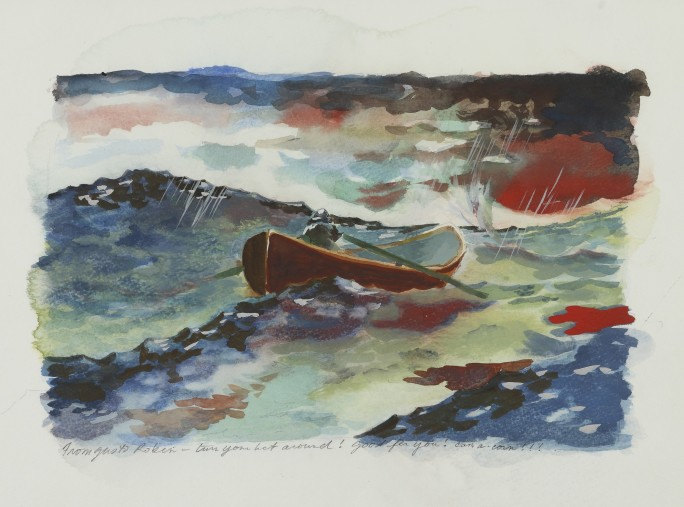
\includegraphics[width = 12cm]{boat_under_storm}
	\caption{{\sc Robin Williams}'s Prized Memento from \href{https://www.imdb.com/title/tt0119217}{\it Good Will Hunting} (1997).}
	\label{fig6}
\end{figure}
{\it Have you ever noticed that there is the phrase ``logical'' at the tail end of the term ``psychological'', which seems to treat nonsense{\tt/}non-logical arguments{\tt/}events{\tt/}situations from human bullshit after its logical counterpart seems so useless?} If anything is not logical{\tt/}does not make sense in the 1st place, you should consider it with the psychological point of view instead, then perhaps it will be even more ``logical''\footnote{Like {\it strong solutions} vs. {\it generalized solutions} in the field of \href{https://en.wikipedia.org/wiki/Partial_differential_equation}{Partial Differential Equations} (PDEs).}.

\subsection{On conscious mind vs. subconscious mind -- Bàn về ý thức vs. tiềm thức}
\textbf{\textsf{Resources -- Tài nguyên.}}
\begin{enumerate}
	\item \cite{Murphy_subconscious}. {\sc Joseph Murphy}. {\it The Power of Subconscious Mind}.
	\item \cite{Murphy_subconscious_VN}. {\sc Joseph Murphy}. {\it The Power of Subconscious Mind -- Sức Mạnh Tiềm Thức}.
\end{enumerate}
Nếu bạn biết sơ về khái niệm về {\it tổng trực tiếp} (direct sum) của Đại số tuyến tính (Linear algebra) trong chương trình Toán cho sinh viên Đại học (Undergraduate Mathematics) thì bạn sẽ hiểu ngay mô tả vắn tắt sau:
\begin{equation}
	\label{conscious + subconscious}
	\tag{mind}
	\mbox{Mind} = \mbox{Conscious Mind}\oplus\mbox{Subconscious Mind},\ \mbox{Tâm thức} = \mbox{Ý Thức}\oplus\mbox{Tiềm Thức}
\end{equation}
Còn nếu bạn đã biết quá rành về khái niệm này, cho phép 2 tác giả xin lỗi vì đã múa rìu qua mắt thợ. Dù sao đi chăng nữa, điều đó không quan trọng lắm, vì mục đích của chúng tôi ở đây là cố gắng mô tả mối tương quan của 2 khía cạnh trong Tâm thức của não bộ loài người là Ý thức (Conscious Mind) \& Tiềm thức (Subconscious Mind). Ý thức điều khiển những việc ta chủ động \& được điều khiển bởi ý chí của ta. Nhưng điều đó không có nghĩa là những hành động tạo bởi Ý thức đều chắc chắn là những hành động thông minh, sáng suốt, thuần logic. Điều đó lại được quyết định bởi cách tư duy \& nhận thức của 1 người chi phối Ý thức hệ của họ. Còn Tiềm thức thì khác, các hoạt động được điều khiển bởi tiềm thức thường nằm sâu bên dưới, thường là lúc ngủ hoặc lúc ta không để ý. 1 cách ví von, khi bạn chạy, Ý thức quyết định việc chuyển động của chân \& tay của bạn, nhưng khi bạn muốn dừng lại, thì Tiềm thức là cái quán tính theo sau ngay đó \& tiếp tục làm việc ở mode background như ở hệ điều hành Unix{\tt/}Linux (operating system, abbr., OS). Việc kiểm soát ý thức hệ sẽ cải thiện đáng kể về các hành động điều khiển bởi Ý thức, nhưng nếu bạn có thể tận dụng Tiềm thức, khiến nó tác động lên các hoạt động này trong 1 thời gian dài theo 1 cách ngấm ngầm. Hoạt động đó sẽ được nâng lên 1 tầm cao hoàn toàn mới. Nguyên lý triết học ở đây là đủ sự thay đổi về lượng sẽ dẫn tới sự thay đổi về chất. Việc thay đổi về lượng là việc tinh chỉnh các tiểu tiết nhỏ nhặt của thói quen (\cite{Clear_habit,Clear_habit_VN,Duhigg_habit,Duhigg_habit_VN}) khiến chúng thay đổi mỗi lần 1 ít, 1 lượng nhỏ. Nhưng nhiều hạt cát nhỏ sẽ tạo thành 1 đống cát to, \& nhiều đống cát to sẽ tạo thành sa mạc. Khi đó Tiềm thức sẽ là thứ chi phối sự thay đổi giữa các nền tảng (platform) hoặc trình độ ở 1 đẳng cấp khác (a whole new level) của 1 hành động bất kỳ.

\subsection{On winning vs. losing -- Bàn về thắng vs. thua}

\begin{quote}
	{\sf Hồng [25; loser]}: I just lost again. {\it What should I do?}
	
	{\sf Hồng [28; philosopher]}: It is alright. You cannot win all the battles in your whole life. If you can, teach me then. After having lost, you need to ask yourself: {\it How did we lose? \& Why did we lose?} Only when you try to reflect yourself in order to answer these questions, you can win some of battles after that painful but useful defeat. Let your enemy become your teacher. Let your enemy help you, teach you, harden you, \& help you harden yourself.
\end{quote}

\begin{quotation}
	{\it``Người không được hèn, nhưng cũng không thể không biết kính sợ, phải biết kính sợ đối thủ của mình.''} -- {\sc Tư Mã Ý}
	
	{\it``Thua mà không đau, thua mà không nhục, cái cần học trước tiên là giỏi thua.''} -- {\sc Tư Mã Ý}
	
	{\it``What will you do? Rebuild it. Just the way it was. Brick for brick.''} -- Dark Knight Trilogy directed by Director {\sc Christopher Nolan}
\end{quotation}

%------------------------------------------------------------------------------%

\section{A Bullshit Theory on Living -- 1 Thuyết Nhảm Nhí Về Việc Sống}
\label{sect: bullshit theory on live}

\begin{quotation}\it
	``No matter what anybody tells you, words \& ideas can change the world.'' -- {\sc Tom Schulman}, \href{https://www.imdb.com/title/tt0097165}{Dead Poets Society} (1989)
\end{quotation}
{\sf Tạm dịch}: Bất luận ai nói gì với bạn đi nữa, ngôn từ \& ý tưởng có thể thay đổi cả thế giới.

\subsection{Love, Death, Robots, \& Artificial Intelligence -- Tình yêu, cái chết, người máy, \& Trí tuệ nhân tạo}
Tên của phần này được lấy cảm hứng từ series film \href{https://www.imdb.com/title/tt9561862}{\it Love, Death \& Robots} (2019--) của nhà sáng tác {\sc Tim Miller} với phần mở rộng là Trí tuệ nhân tạo (AI) trong thời đại AI bắt đầu chiếm lĩnh trên khắp các lĩnh vực của cuộc sống con người.

\noindent\textbf{\textsf{Resources -- Tài nguyên.}}
\begin{enumerate}
	\item \cite{Aoun_robot-proof}. {\sc Joseph E. Aoun}. {\it Robot-Proof: Higher Education in the Age of Artificial Intelligence}.
	
	Với bản dịch tiếng Việt:
	\item \cite{Aoun_robot-proof_VN}. {\sc Joseph E. Aoun}. {\it Robot-Proof: Higher Education in the Age of Artificial Intelligence -- Chạy Đua Với Robot: Học Tập Thời Trí Tuệ Nhân Tạo}.
\end{enumerate}

\begin{flushright}
	\musEighth[\href{https://www.youtube.com/watch?v=dIbeazAlxM4}{\small{\sc Chopin} {\it Ballade No. 1 in G Minor}}]\musEighth
\end{flushright}
18 tuổi. Sinh viên năm nhất Đại học. Khoa Toán Tin. Nhưng ít khi nào hắn đến lớp. Hắn phải chạy về quê liên tục. Chạy lên chạy về. Khối ung thư gan tưởng chừng lành tính của cha hắn giờ chuyển sang ác tính, không còn cứu vãn nổi. Bác sĩ lắc đầu, trả cha hắn về nhà, cốt để sống nốt những ngày còn sót lại trên đời. Hắn vẫn ngồi học bên cạnh giường bệnh của cha hắn. Death bed thì đúng hơn. Hắn đang cố tính toán hay giải 1 bài toán gì đấy trong quyển {\it Calculus} dày cộm của {\sc James Stewart} trên chiếc máy tính bảng nhỏ. Cha hắn đau khắp người, cố gắng trở mình thật nhẹ để dò 1 vị trí nằm đỡ đau hơn nhưng sau khi thử nghiệm 1 hồi thì bất thành. Chả có cách nào bớt đau cả. Ung thư mà. Cơ bắp \& thịt thà bốc hơi. Cơ thể cha hắn khô héo, ốm tong ốm teo, chỉ trừ cái bụng to như cóc chữa do tràn nước dịch gan. Hắn ghét điều này nhưng phải thừa nhận: Cha hắn chưa bao giờ lo cho hắn tới nơi tới chốn nhưng ông ta đã cố hết sức có thể. Sự bất lực của cha hắn trong việc làm cha lại xuất phát từ cha của cha hắn, tức ông nội hắn, \& mẹ của cha hắn, tức bà nội hắn. Ngắn gọn thế này: Nếu bà nội hắn có $n\in\mathbb{N}^\star$ người con với $n\ge2$, với cha hắn là con trưởng, thì mẹ của cha hắn sẽ thương $n - 1$ người còn lại \& cố bòn rút tài sản từ cha hắn để san cho $n - 1$ người em đó, thậm chí 2 đứa con thơ của người con cả đó có nheo nhóc cỡ nào đi chăng nữa thì cũng mặc kệ. Sống chết mặc bây: Tao vai mẹ. Tao chả cần biết. Tao đách quan tâm. Còn nếu $n = 1$ thì bà nội hắn sẽ nhận con nuôi hoặc thương con của hàng xóm. Còn ông nội hắn đào ngũ trong chiến tranh, nghiện tình dục, \& vô trách nhiệm. 1 đống con ngoài giá thú nhưng ít ai gọi ông ta là cha. 1 đống tình nhân không thèm nhìn mặt: hận thấu xương tủy. Rõ ràng đấy là nguyên nhân chính khiến mẹ của cha hắn trút hết sự thù hận từ người chồng lên đứa con đầu lòng. Cha hắn cả 1 đời thiếu thốn tình thương từ cha mẹ \& người vợ trước cho tới tận lúc lìa đời, nên đến lúc làm cha dẫu vẫn cố gắng bao nhiêu cũng không thể bày tỏ cảm xúc. Cha hắn học dốt, bày tỏ cảm xúc còn dốt hơn. Hắn tự học vẽ, thi vẽ nhất nhì tỉnh, cha hắn im. Hắn tự học toán, thi toán nhất nhì tỉnh, cha hắn vẫn im. Đợi hắn đi khỏi nhà thì cha hắn đeo cái tấm Huy chương vàng Olympic 30.4 miền Nam khoe khắp hàng xóm: ``Thằng con tui đấy!'' Mãi tận sau này hắn mới nghe mẹ hắn kể lại chuyện đấy. Ngu xuẩn về chỉ số thông minh cảm xúc -- Super low on Emotion Quotient (EQ): Cả 2 cha con. Vừa ảnh hưởng môi trường, hoàn cảnh, vừa ảnh hưởng nhờ di truyền. Tuyệt nhiên không lẫn vào đâu được.

Thời điểm cha hắn vừa chết, hắn như vỡ òa, lết cái thân như người mất hồn ra vườn kiếm mẹ: ``Cha ổng đi rồi mẹ ơi. Mẹ lên coi thử.'' mẹ hắn cắt 1 nải chuối xanh để lên ngực của xác cha hắn, đúng hủ tục truyền thống dưới quê. Những người mai táng cho cha hắn vào 1 cái bao, có vài phần nhô ra, họ liền thẳng tay bẻ phần xương đó răng rắc cho khớp với cái bao. Chỉ là 1 mớ xương, máu, thịt, \& chất dịch. {\it Sao lại làm hắn khổ sở đến thế?} Hắn chả còn muốn đến trường. Chả có ai để mà hắn khoe chiến tích nữa. Mẹ hắn cũng chả hiểu giải đặc biệt Olympic Toán toàn quốc là gì. Bà trầm cảm vì thành góa phụ mất chồng nên chả thèm trả lời hắn. Không thể trả lời thì đúng hơn. 1 gia đình ít học, ít hiểu biết, \& ít vốn kiến thức ở 1 chốn hoang vu như rừng sâu, thiếu hụt những sự tiện nghi vật chất, \& những tiến bộ kỹ thuật của thế giới bên ngoài.

Trước khi cha hắn chết, thoi thóp chỉ để ráng nói 1 câu: ``Ráng $\ldots$ sống $\ldots$ có $\ldots$ đức.'' {\it Cái kiểu di chúc quái quỷ gì thế này?} Rồi ánh mắt dần đục hẳn. 1 linh hồn vừa thoát khỏi cái xác vật lý ở không gian vật lý 3 chiều $\mathbb{R}^3$ rồi chui tọt vào cõi tâm linh hay cõi linh hồn gì đấy, nói chung là spirituality realm. Hắn chả rành mấy cái bên spirituality.

Đến thầy Quí dạy Toán cấp 3 cho hắn, trước khi chết cũng tìm đến hắn. Hắn chả hiểu. Hắn có để ý tới bài giảng của thầy Quí đâu. Hắn toàn kiểu tự học, không cần ai quan tâm. Sao những người trước khi chết đều tìm đến hắn để hy vọng sau này hắn sẽ trở thành cái gì đấy. Hắn là cái thể loại khó ưa. Lúc nào cũng im im. Dẫu có tốt nhưng chỉ biết giấu trong bụng mà không biết thể hiện cảm xúc. Thầy cô hắn quý hắn chỉ vì tài, chứ nếu xét về tình cảm thì chắc chắn chả bao giờ họ thèm đếm xỉa tới cái thể loại thiểu năng trí tuệ cảm xúc như hắn.

{\it``Họ thấy cái quái quỷ gì ở mình nhỉ?''} -- Hắn tự hỏi mãi câu hỏi ấy. Sau này hắn mới lờ mờ nhận ra câu trả lời. Chính cái sự chính trực đến mức làm người khác khó chịu của hắn sẽ khiến hắn lận đận trong phần lớn thời gian suốt cuộc đời hắn, nhưng tới 1 lúc nào đó, khi đạt đến 1 ngưỡng bão hòa về đau khổ đến mức được khai minh, thức tỉnh nhất định, hắn sẽ tự biết cái sứ mệnh chết tiệt của hắn là gì. {\it Sống có đức để rồi bị mấy thể loại thầy cô ganh tỵ với tài năng của hắn chửi hắn vô đạo đức hay có tài mà không có đức? Sống có tài để rồi bị lợi dụng bởi mấy thể loại bất tài \& vô đạo đức?} Toàn những kiểu sống chả đâu tới đâu. Toàn phải chịu lỗ. Toàn chỉ biết tự hại bản thân. Fucking inevitable (?) self-destruction{\tt/}self-sabotage.

1 quy luật của thế giới tự nhiên về các quần xã động vật: 1 cá thể non nớt khi bị ép buộc phải vào đời, bị quăng vào xã hội khắc nghiệt, đầy phức tạp mà không có sự giúp đỡ từ cha mẹ thì sẽ gần như đồng nghĩa với việc chắn chắc cá thể đó sẽ phải chết. Chỉ có 1 xác suất cực nhỏ là sẽ xuất hiện 1 vài cá thể ngoại lai (outliers) đủ kiên cường vượt qua quá trình sinh tồn khắc nghiệt đó mà không bị biến chất hay hắc hóa.

Khoan đã, nhưng tại sao lại phải theo chủ nghĩa phân cực polarism nhể? Hắn chỉ cần sống có đức với những người xứng đáng cái đức, cái lòng tốt của hắn, \& hắn sống có tài để lấy cái tài tác động đến những người cần cái tài của hắn. Nếu ai đó xứng đáng cả 2 thì hắn sẽ trao cho cả 2. Oh, that is it: the fucking ``blending principle'' in OpenFOAM \& in Fluid Dynamics:

\begin{Rule}[Blending linear combinations \& generalizations]
	Khi bạn có nhiều lựa chọn $A_i$ với $i = 1,2,\ldots,n\in\mathbb{N}^\star$, thay vì suy nghĩ phiến diện hoặc cực đoan chỉ chọn 1 hay 1 vài trong số chúng, hãy (thử) chọn 1 tổ hợp tuyến tính (linear combination, see, e.g., {\rm\cite{Hung_linear_algebra,Trefethen_Bau1997,Trefethen_Bau2022}}) gồm tất cả các lựa chọn đó, i.e., $\sum_{i = 1}^n c_iA_i$ với các hệ số $c_i > 0$ thỏa mãn $\sum_{i = 1}^n c_i = 1$ \& mỗi hệ số $c_i$ phải được chặn dưới bởi ngưỡng cực tiểu $c_{i,\min}$ (minimum threshold), i.e., $c_{i,\min}\le c_i$, \& chặn trên bởi ngưỡng cực đại (maximum threshold) $c_{i,\max}$, i.e., $c_i\le c_{i,\max}$, gom cả 2 lại thành $c_i\in[c_{i,\min},c_{i,\max}]$. Luôn cố gắng giữ các hệ số trong khoảng này để tránh trường hợp khai thác không đủ tốt, i.e., $c_i < c_{i,\min}$ hoặc quá lạm dụng (abusive), i.e., $c_i > c_{i,\max}$. Luôn tinh chỉnh không ngừng các hệ số $c_i$ để dò tìm tổ hợp tuyến tính tối ưu cho từng hoàn cảnh, trường hợp cụ thể để xây dựng hệ thống kinh nghiệm tương ứng với 1 phổ ứng dụng các trường hợp đã, đang, \& sẽ xảy ra. Nếu (các) lựa chọn $A_i$ nào đó có tác hại thì cứ xét $c_i < 0$ vẫn thêm các ngưỡng $c_{i,\min},c_{i,\max}$ tương ứng để luôn kiểm soát sự cân bằng. Đừng ngần ngại phá vỡ ranh giới của tính sự tuyến tính, xét tổ hợp phi tuyến (nonlinear combination) nếu cần thiết.
\end{Rule}

\subsection{Heavens on Earth -- Các thiên đàng trên thế gian}
\begin{quote}
	{\it``The destiny of man lies in his soul.''} -- {\sc Herodotus}, \cite[p. 1]{Adler_human_nature}
	
	-- ``Vận mệnh của 1 người đã được định sẵn trong linh hồn anh ta.'' -- -- {\sc Herodotus}, \cite[p. 4]{Adler_human_nature_VN}
\end{quote}
\textbf{\textsf{Resources -- Tài nguyên.}}
\begin{enumerate}
	\item \cite{Hanh_silence}. {\sc Thích Nhật Hạnh}. {\it Silence: The Power of Quiet in a World Full of Noise}.\footnote{Amazon link: \url{https://www.amazon.com/Silence-Power-Quiet-World-Noise/dp/0062224697}.}	
	\begin{quotation}
		{\it``Consciously choosing what \& who you surround yourself with is among the keys to finding more space for joy.''}
		
		-- Lựa chọn một cách có ý thức những người xung quanh bạn là một trong những chìa khóa để tìm thêm không gian cho niềm vui.
		
		{\it``Am I doing what I most want to be doing with my life? Do I even know what that is?''}
		
		-- Tôi có đang làm điều tôi muốn làm nhất trong đời mình không? Tôi thậm chí có biết đó là gì không?
		
		{\it``The 2nd sound is the Sound of the One Who Observes the World. This is the sound of listening, the sound of silence.''}
		
		-- Âm thanh thứ hai là Âm thanh của Người quan sát thế giới. Đây là âm thanh của sự lắng nghe, âm thanh của sự im lặng.
	\end{quotation}
	Với bản dịch tiếng Việt:
	\item \cite{Hanh_silence_VN}. {\sc Thích Nhật Hạnh}. {\it Silence -- Tĩnh Lặng: Sức Mạnh Tĩnh Lặng Trong Thế Giới Huyên Náo}.
	\item \cite{Ruiz_4_agreements}. {\sc don Miguel Ruiz}. {\it The Four Agreements: A Practical Guide to Personal Freedom (A Toltec Wisdom Book)}.
	
	Với bản dịch tiếng Việt:
	\item \cite{Ruiz_Mills_4_agreements_VN}. {\sc don Miguel Ruiz, Janet Mills}. {\it The Four Agreements: A Practical Guide to Personal Freedom (A Toltec Wisdom Book) -- 4 Thỏa Ước: Bí Quyết Sống Tự Do, Bình An, Hạnh Phúc Giữa Thế Giới Bất Định}.
	\item \cite{Ruiz_Ruiz_5th_agreement}. {\sc don Miguel Ruiz, don Jose Ruiz, Janet Mills}. {\it The Fifth Agreement: A Practical Guide to Self-Mastery (A Toltec Wisdom Book)}.
	\item \cite{Ruiz_mastery_self}. {\sc don Miguel Ruiz Jr.} {\it The Mastery of Self: A Toltec Guide to Personal Freedom (Toltec Mastery Series)}.\footnote{Amazon link: \url{https://www.amazon.com/Mastery-Self-Toltec-Personal-Freedom/dp/1938289692}.}
	\begin{quotation}
		{\it``Self-domestication is the act of accepting ourselves on the condition that we live up to the ideals we have adopted from others in the Dream of the Planet, without ever considering if those ideals are what we truly want.''}
		
		-- Tự thuần hóa là hành động chấp nhận bản thân với điều kiện chúng ta phải sống theo những lý tưởng mà chúng ta đã tiếp nhận từ những người khác trong Giấc mơ về Hành tinh mà không bao giờ cân nhắc xem liệu những lý tưởng đó có phải là điều chúng ta thực sự mong muốn hay không.
				
		{\it``You become a Master of Self when you can engage the Dream of the Planet \& everyone in it without losing sight of your Authentic Self, \& while maintaining the awareness that every choice you make is your own.''}
		
		-- Bạn trở thành Bậc thầy của Bản thân khi bạn có thể tham gia vào Giấc mơ của Hành tinh \& mọi người trong đó mà không đánh mất Con người Đích thực của mình, \& trong khi duy trì nhận thức rằng mọi lựa chọn bạn đưa ra đều là của riêng bạn.
		
		{\it``An attachment is the action of taking something that is not a part of you \& making it a part of you through an emotional or energetic investment.''}
		
		-- Sự gắn bó là hành động lấy đi thứ gì đó không phải là một phần của bạn \& biến nó thành một phần của bạn thông qua một sự đầu tư đầy cảm xúc hoặc năng lượng.
		
		{\it``I am responsible for what I say, but I am not responsible for what you hear.''}
		
		-- Tôi chịu trách nhiệm về những gì tôi nói, nhưng tôi không chịu trách nhiệm về những gì bạn nghe.
		
		{\it``This is what resentment is: self-inflicted suffering with the emotional poison we wish for another.''}
		
		-- Đây chính là sự oán giận: sự đau khổ tự gây ra bằng chất độc cảm xúc mà chúng ta mong muốn cho người khác.
	\end{quotation}
	Với bản dịch tiếng Việt:
	\item \cite{Ruiz_mastery_self}. {\sc don Miguel Ruiz Jr.} {\it The Mastery of Self: A Toltec Guide to Personal Freedom (Toltec Mastery Series) -- The Mastery of Self: A Toltec Guide to Personal Freedom (Toltec Mastery Series) -- Hành Trình Thấu Hiểu Bản Thân \& Tìm Thấy Tự Do}.
	\item \cite{Tolle_oneness}. {\sc Eckhart Tolle}. {\it Oneness With All Life}.
	
	Với bản dịch tiếng Việt:
	\item \cite{Tolle_oneness_VN}. {\sc Eckhart Tolle}. {\it Oneness With All Life -- Hợp Nhất với Vũ Trụ}.
	\item \cite{Tolle_now}. {\sc Eckhart Tolle}. {\it The Power of Now: A Guide to Spiritual Enlightenment}. Với bản dịch tiếng Việt:
	\item \cite{Tolle_now_VN}. {\sc Eckhart Tolle}. {\it The Power of Now: A Guide to Spiritual Enlightenment -- Sức Mạnh của Hiện Tại}.
	\item \cite{Tolle_practice_now}. {\sc Eckhart Tolle}. {\it Practicing The Power of Now: Essential Teachings, Meditations, \& Exercises From The Power of Now}.
	\begin{quotation}
		{\it``Realize deeply that the present moment is all you ever have. Make the Now the primary focus of your life.''}
		
		-- Hãy nhận thức sâu sắc rằng khoảnh khắc hiện tại là tất cả những gì bạn có. Hãy biến cái Hiện tại thành trọng tâm chính trong cuộc đời bạn.
		
		{\it``The single most vital step on your journey toward enlightenment is this: Learn to disidentify from your mind. Every time you create a gap in the stream of mind, the light of your consciousness grows stronger.''}
		
		-- Bước quan trọng nhất trên hành trình hướng tới giác ngộ của bạn là: Học cách loại bỏ sự đồng nhất khỏi tâm trí của bạn. Mỗi khi bạn tạo ra một khoảng trống trong dòng tâm thức, ánh sáng ý thức của bạn ngày càng mạnh mẽ hơn.
		
		{\it``The beginning of freedom is the realization that you are not the possessing entity -- the thinker. Knowing this enables you to observe the entity. The moment you start watching the thinker, a higher level of consciousness becomes activated.''}
		
		-- Sự khởi đầu của tự do là việc nhận ra rằng bạn không phải là thực thể sở hữu - người suy nghĩ. Biết được điều này cho phép bạn quan sát thực thể. Khoảnh khắc bạn bắt đầu quan sát người suy nghĩ, mức độ ý thức cao hơn sẽ được kích hoạt.
	\end{quotation}
	Với bản dịch tiếng Việt:
	\item \cite{Tolle_practice_now_VN}. {\sc Eckhart Tolle}. {\it Practicing The Power of Now -- Trải Nghiệm Sức Mạnh Hiện Tại}.
	\item \cite{Tolle_earth_VN}. {\sc Eckhart Tolle}. {\it A New Earth: Awakening to Your Life's Purpose -- Thức Tỉnh Mục Đích Sống}.
	\item \cite{Tolle_stillness_VN}. {\sc Eckhart Tolle}. {\it Stilless Speaks -- Sức Mạnh của Tĩnh Lặng}.
	\item \cite{Frankl_meaning,Frankl_meaning_revised}. {\sc Viktor Emil Frankl}. {\it Man's Search For Meaning}.
	\begin{quotation}
		{\it``Life ultimately means taking the responsibility to find the right answer to its problems \& to fulfill the tasks which it constantly sets for each individual.''}
		
		-- Cuộc sống suy cho cùng có nghĩa là có trách nhiệm tìm ra câu trả lời đúng đắn cho những vấn đề của mình \& để hoàn thành những nhiệm vụ mà nó không ngừng đặt ra cho mỗi cá nhân.
		
		{\it``Emotion, which is suffering, ceases to be suffering as soon as we form a clear \& precise picture of it.''}
		
		-- Cảm xúc, tức là đau khổ, sẽ ngừng đau khổ ngay khi chúng ta hình thành một bức tranh rõ ràng \& chính xác về nó.
		
		{\it``If there is a meaning in life at all, then there must be a meaning in suffering. Suffering is an ineradicable part of life, even as fate \& death. Without suffering \& death human life cannot be complete.''}
		
		-- Nếu cuộc sống có ý nghĩa gì đó thì đau khổ cũng phải có ý nghĩa. Đau khổ là một phần không thể xóa bỏ được của cuộc sống, kể cả số phận và cái chết. Không có đau khổ và cái chết, cuộc sống con người không thể trọn vẹn.
	\end{quotation}
	Với bản dịch tiếng Việt:
	\item \cite{Frankl_meaning_VN}. {\sc Viktor Emil Frankl}. {\it Man's Search For Meaning -- Đi Tìm Lẽ Sống}.
	\item \cite{Adler_science_living}. {\sc Alfred Adler}. {\it The Science of Living}.
	\begin{quotation}
		{\it``Curiously enough we will find that no 2 children, even those born in the same family, grow up in the same situation. Even within the same family the atmosphere that surrounds each individual child is quite particular. Thus the 1st child has notoriously a different set of circumstances from the other children. The 1st child is at 1st alone \& is thus the center of attention. Once the 2nd child is born, he finds himself dethroned \& he does not like the change of situation. In fact it is quite a tragedy in his life that he has been in power \& is so no longer. This sense of tragedy goes into the formation of his prototype \& will crop out in his adult characteristics.''}
		
		-- Thật kỳ lạ, chúng ta sẽ thấy rằng không có 2 đứa trẻ nào, kể cả những đứa trẻ sinh ra trong cùng một gia đình, đều lớn lên trong hoàn cảnh giống nhau. Ngay cả trong cùng một gia đình, bầu không khí xung quanh mỗi đứa trẻ cũng khá đặc biệt. Vì vậy, đứa trẻ đầu tiên nổi tiếng là có hoàn cảnh khác với những đứa trẻ khác. Đứa con thứ nhất đứng đầu một mình \& nên là trung tâm của sự chú ý. Khi đứa con thứ 2 chào đời, anh thấy mình bị truất ngôi \& anh không thích sự thay đổi của hoàn cảnh. Trên thực tế, đó là một bi kịch trong cuộc đời anh ta khi anh ta đã nắm quyền \& không còn nữa. Cảm giác bi kịch này đi vào quá trình hình thành nguyên mẫu của anh ấy \& sẽ thể hiện những đặc điểm trưởng thành của anh ấy.
		
		{\it``Nature is so rich \& the possibilities of stimuli, instincts, \& mistakes are so numerous, that it is not possible for 2 persons to be exactly identical.''}
		
		-- Thiên nhiên rất phong phú \& khả năng kích thích, bản năng, \& sai lầm nhiều đến mức không thể có 2 người giống hệt nhau được.
		
		{\it``Another fact to be borne in mind in connection with criminals is that if we increase the punishments, so far from frightening the individual criminal, we merely help to increase his belief that he is a hero. We must not forget that the criminal lives in a self-centered world, a world in which one will never find true courage, self-confidence, communal sense, or understanding of common values. It is not possible for such persons to join a society. Neurotics seldom start a club, \& it is an impossible feat for persons suffering from agoraphobia or for insane persons. Problem children or persons who commit suicide never make friends, a fact for which the reason is never given. There is a reason, however: they never make friends because their early life took a self-centered direction. Their prototypes were oriented towards false goals \& followed lines of direction on the useless side of life.''}
		
		-- Một thực tế khác cần lưu ý liên quan đến tội phạm là nếu chúng ta tăng các hình phạt, thay vì khiến cá nhân tội phạm sợ hãi, chúng ta chỉ giúp tăng cường niềm tin của anh ta rằng anh ta là anh hùng. Chúng ta không được quên rằng tội phạm sống trong một thế giới lấy bản thân làm trung tâm, một thế giới mà người ta sẽ không bao giờ tìm thấy lòng dũng cảm thực sự, sự tự tin, ý thức cộng đồng hoặc sự hiểu biết về các giá trị chung. Những người như vậy không thể gia nhập một xã hội. Những kẻ thần kinh hiếm khi thành lập một câu lạc bộ, \& đó là một kỳ tích không thể thực hiện được đối với những người mắc chứng sợ khoảng rộng hoặc những người mất trí. Những đứa trẻ có vấn đề hoặc những người tự tử không bao giờ kết bạn, một sự thật mà lý do không bao giờ được đưa ra. Tuy nhiên, có một lý do: họ không bao giờ kết bạn vì cuộc sống ban đầu của họ có hướng ích kỷ. Nguyên mẫu của họ hướng tới những mục tiêu sai lầm \& đi theo những hướng đi về phía vô ích của cuộc sống.
	\end{quotation}
	\item \cite{Adler_human_nature}. {\sc Alfred Adler}. {\it Understanding Human Nature}.
	
	\item \cite{Adler_human_nature_VN}. {\sc Alfred Adler}. {\it Understanding Human Nature -- Hiểu Về Bản Chất Con Người}.
	\item {\sc Alfred Adler}. {\it What Life Should Mean To You}.
	\item {\sc Alfred Adler}. {\it The Case of Miss R: The Interpretation of A Life Story}.
	\item \cite{Wiest_101_essays}. {\sc Brianna Wiest}. {\it 101 Essays That Will Change The Way You Think}.
	\begin{quotation}
		{\it``Accomplishing goals is not success. How much you expand in the process is.''}
		
		-- Hoàn thành các mục tiêu không phải là thành công. Mà việc bạn mở rộng bao nhiêu trong quá trình này mới là thành công.
		
		{\it``Your habits create your mood, \& your mood is a filter through which you experience your life.''}
		
		-- Thói quen của bạn tạo ra tâm trạng của bạn, \& tâm trạng của bạn là một bộ lọc để bạn trải nghiệm cuộc sống của mình.
		
		{\it``You must learn to let your conscious decisions dictate your day -- not your fears or impulses.''}
		
		-- Bạn phải học cách để những quyết định có ý thức quyết định ngày của bạn -- chứ không phải nỗi sợ hãi hay sự bốc đồng của bạn
	\end{quotation}	
	Với bản dịch tiếng Việt:
	\item \cite{Wiest_101_essays_VN}. {\sc Brianna Wiest}. {\it 101 Essays That Will Change The Way You Think -- Sống Khai Vấn, Sống Tỉnh Thức}.
\end{enumerate}

\begin{question}
	What is living? Why do we live? What to live for? Who to live with? How to live?
	
	-- Sống là gì? Tại sao ta sống? Ta sống vì điều gì? Ai mà ta sống chung với? Sống thế nào?
\end{question}
The authors devote this section to extend some aspects in some humble senses, with all respects, the theory of {\it Adlerian psychology} proposed by the Austrian psychiatrist {\sc Alfred Adler}.

The main sources are \cite{Adler_science_living}.

Instead of keeping \& waiting to open the blackholes as a psychological manipulators to suck all the positivities \& spread all negativities, people should open the heaven gate on Earth to spread all positivities \& destroy all negativities that make human beings keep suffering.

\begin{Rule}[On stupidity -- Bàn về sự ngu dốt]
	Take responsibility of your stupidity. Do not let your stupidity, no matter if you are aware of it or not, harm or even destroy any person in the aspect of either his{\tt/}her (private) personal life or professional career or both.
	
	-- Chịu trách nhiệm cho sự ngu dốt của bạn. Đừng để sự ngu dốt của bạn, dù bạn có nhận thức được nó hay không đi nữa, làm hại hoặc hủy hoại bất cứ ai trong khía cạnh cuộc sống cá nhân (riêng tư) \&{\tt/}hoặc sự nghiệp của người đó.
\end{Rule}


Maps of Meanings.

Let's hunt some low self-esteem.

Let's cook.

\begin{center}\it
	{\sc Life's recipe}
	
	A little bit of trusts. A little bit of betrayals.
	
	A little bit of loves. A little bit of denials.
\end{center}

\begin{Rule}[On deserving responsibility -- Bàn về sự xứng đáng về trách nhiệm] 
	Only take responsibility for whom deserved your responsibility.
	
	-- Chỉ chịu trách nhiệm cho ai xứng đáng với trách nhiệm của bạn.
\end{Rule}

\subsubsection{On fragility vs. hardening process -- Bàn về sự mong manh vs. quá trình cường hóa}

\begin{quote}
	{\sf Thương [25; 2nd year mathematics PhD; sucked at mathematics]}: Hồng như 1 tờ giấy trắng vậy, mong manh dễ vỡ.
	
	{\sf Nhân [23; Master 2 pure mathematics students]} nghĩ trong đầu: {\it Why does this stupid bitch talk so much? Can she just shut the fuck up \& let me alone?} -- Tại sao con đĩ ngu xuẩn, nứng \st{lồn} âm vật mong manh này nói lắm thế? Bộ ả ta không thể câm mồm lại \& để tôi yên được à?
\end{quote}

\begin{example}[Nobel văn học Han Kang]
	On fragility of human beings.
\end{example}

\subsubsection{On joy vs. pain -- Bàn về lạc thú vs. nỗi đau \& cách cân bằng chúng}
\textbf{\textsf{Resources -- Tài nguyên.}}
\begin{enumerate}
	\item \cite{Lembke_dopamine}. {\sc Anna Lembke}. {\it Dopamine Nation: Finding Balance in the Age of Indulgence}.
	\begin{quotation}
		{\it``This book is about pleasure. It's also about pain. Most important, it's about how to find the delicate balance between the two, and why now more than ever finding balance is essential.''}
		
		-- ``Cuốn sách này nói về lạc thú. Nó cũng nói về nỗi đau. Nhưng trên hết, nó nói về mối quan hệ giữa lạc thú \& nỗi đau, cũng như tầm quan trọng của việc hiểu được mối quan hệ đó để sống 1 cuộc đời đúng nghĩa.'' -- \cite[p. 9]{Lembke_dopamine_VN}
		
		{\it``The paradox is that hedonism, the pursuit of pleasure for its own sake, leads to anhedonia, which is the inability to enjoy pleasure of any kind.''}
		
		-- Điều nghịch lý là chủ nghĩa khoái lạc, việc theo đuổi thú vui vì lợi ích riêng của nó, dẫn đến anhedonia, tức là không có khả năng tận hưởng bất kỳ loại khoái cảm nào.
		
		{\it``The reason we're all so miserable may be because we're working so hard to avoid being miserable.''}
		
		-- Lý do khiến tất cả chúng ta đau khổ đến vậy có thể là vì chúng ta đang cố gắng quá nhiều để tránh bị đau khổ.
		
		{\it``Dopamine may play a bigger role in the motivation to get a reward than the pleasure of the reward itself. Wanting more than liking.''}
		
		-- Dopamine có thể đóng một vai trò lớn hơn trong việc tạo động lực để nhận được phần thưởng hơn là niềm vui khi nhận được phần thưởng đó. Muốn nhiều hơn là thích.
	\end{quotation}
	Với bản dịch tiếng Việt:	
	\item \cite{Lembke_dopamine_VN}. {\sc Anna Lembke}. {\it Dopamine Nation: Finding Balance in the Age of Indulgence -- Giải Mã Hoóc-môn Dopamine: Sống Cân Bằng Trong Thời Đại Đầy Cám Dỗ}.
\end{enumerate}

\subsubsection{On betrayal vs. loyalty -- Bàn về sự phản bội vs.{\tt/}\& lòng trung thành}
Nếu bạn có xem phim \href{https://www.imdb.com/title/tt1028532/}{\it Hachi: A Dog's Tale} (2009) kể về chú chó {\sc Hachiko} có thật ở Nhật Bản, bạn sẽ hiểu lòng trung thành (loyalty) là như thế nào. Nhà tôi thích nuôi chó, không biết từ đời nào, chỉ biết là đến giờ mẹ tôi vẫn nuôi vài con, \& tôi yêu tất cả những chú chó từng sống, hiện sống, \& sẽ sống với chúng tôi. Chúng trung thành, quan tâm chủ, tận tụy đi theo theo chủ từ sáng sớm đến tận khuya -- do cha mẹ tôi là nông dân (farmers) \& tôi là con nông dân (farmer boy). Chó còn được dùng như 1 người bạn đồng hành để trị liệu tâm lý cho những người bị chứng rối loạn cảm xúc hoặc mắc chứng trầm cảm. Xem \href{https://en.wikipedia.org/wiki/Therapy_dog}{Wikipedia{\tt/}therapy dog} -- chó trị liệu.

Nếu bạn có cơ hội gặp 1 con chó hoang (stray dog) bị ngược đãi, bạn sẽ hiểu rõ hơn về sự run rẫy, sự sợ hãi, sự đau khổ trước nghịch cảnh cuộc đời của chúng. Khi bạn cho 1 con chó hoang ăn, nó sẽ ít khi nào hoặc sẽ không bao giờ cắn bạn. Nó sẽ vẫy đuôi, nếu còn chút sức lực sót lại, sự hung dữ kích hoạt bởi {\it cơ chế tự vệ} ({\it defending mechanism}) do sợ hãi vì bị ngược đãi trước đây dần dịu đi, ánh mắt cũng dần dịu xuống rồi nhìn bạn 1 cách trìu mến. Tôi thường có thể vuốt ve 1 chú chó hoang 1 cách dễ dàng sau khi gặp chúng trong tầm 10 phút đến nửa tiếng. Trong khoảng thời gian đó, tôi cố thiết lập sự tin tưởng ở chúng đối với tôi. Các người huấn luyện chó nói riêng hoặc động vật nói chung thường hiểu rất rõ ngôn ngữ cơ thể \& ánh mắt dịu dàng, đầy ắp sự quan tâm là 2 trong những điều quan trọng nhất khi tiếp xúc với 1 con vật hoang bị ngược đãi. Chúng mất lòng tin ở cả đồng loại \& ở con người. Bạn cần thời gian để xoa dịu nỗi đau ở chúng. {\it Establish the real trust \& then the loyalty will naturally follow as a reward that you deserve}. It is 1 of the most obvious but easy-to-ignore rule in the natural world of animals. Có thể tôi chỉ là 1 con vật độc ác nào đấy được{\tt/}bị vài người thầy của tôi trước đây ví von như trên kênh Discovery Channel. Nhưng đối với lũ chó hoang thì tôi là ân nhân của chúng.
\begin{figure}[H]
	\centering
	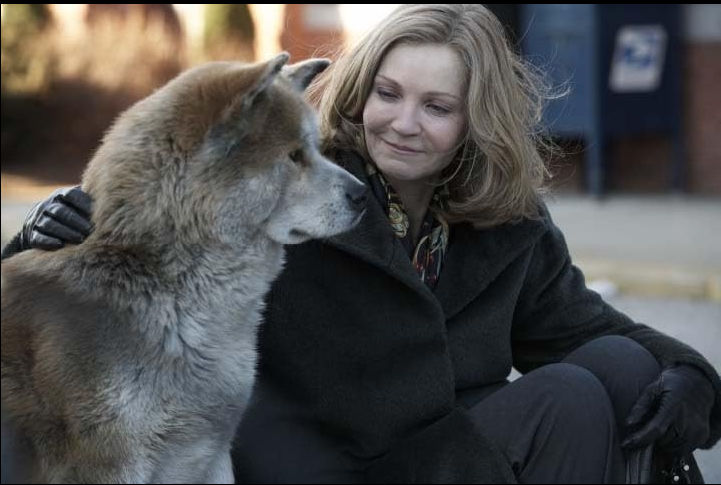
\includegraphics[width = 12cm]{Hachi_wait}
	\caption{A scene in \href{https://www.imdb.com/title/tt1028532/}{\it Hachi: A Dog's Tale} (2009).}
\end{figure}
\begin{figure}[H]
	\centering
	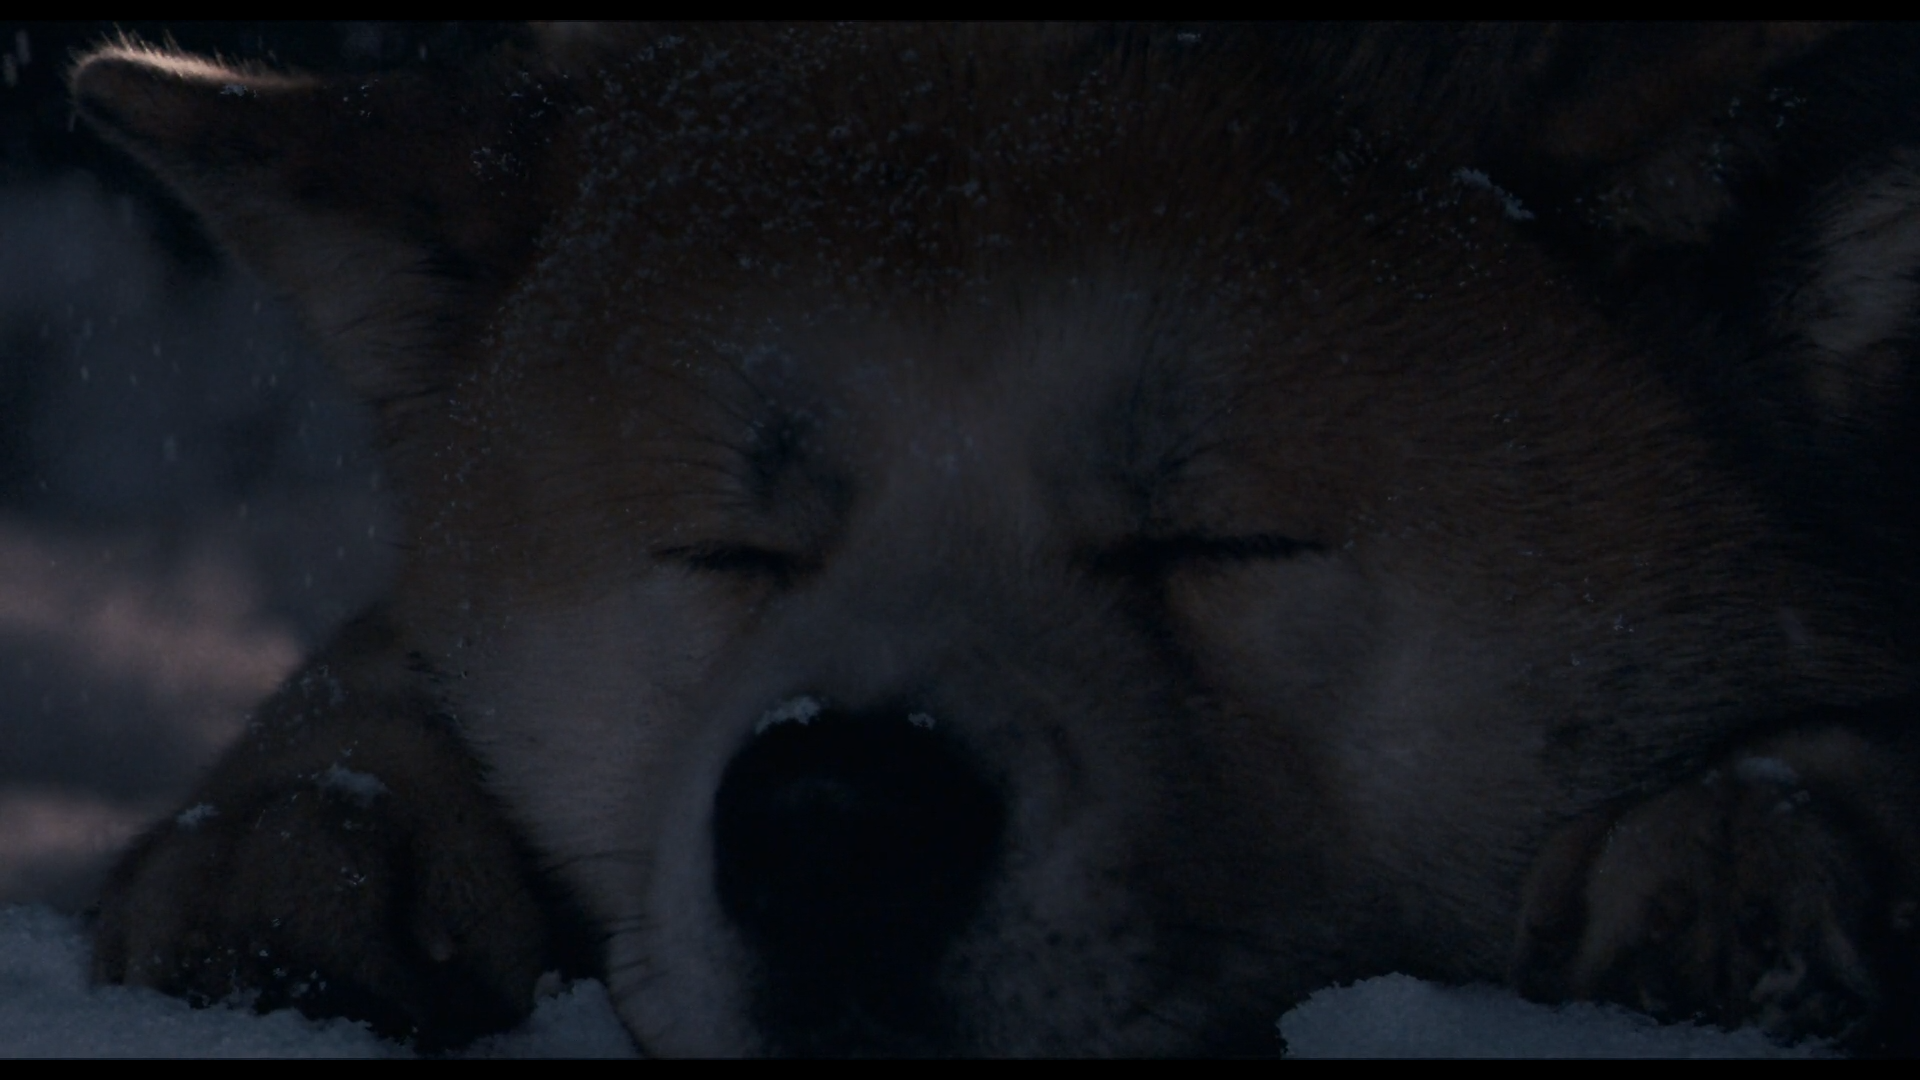
\includegraphics[width = 12cm]{Hachi_die}
	\caption{Hachiko dog dies.}
\end{figure}
\begin{figure}[H]
	\centering
	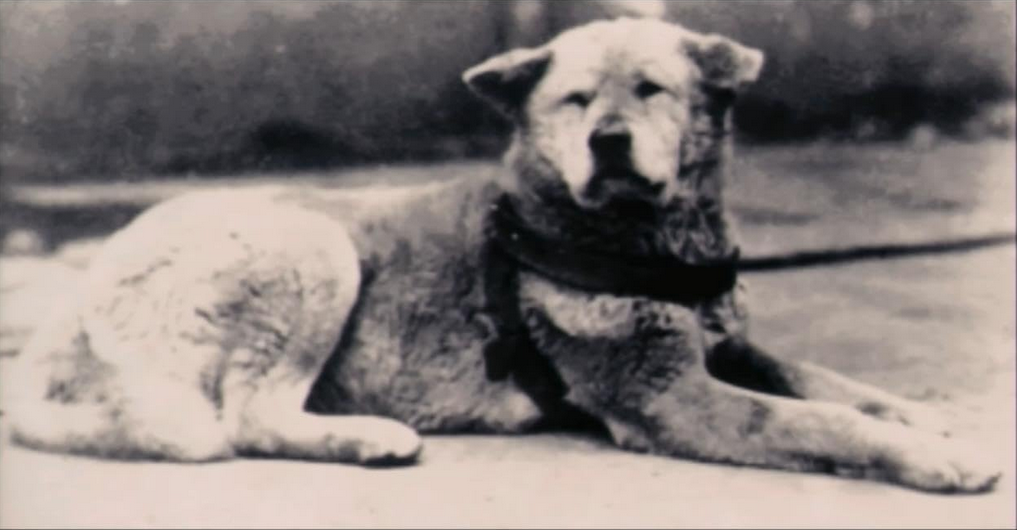
\includegraphics[width = 12cm]{Hachiko}
	\caption{Hachiko dog.}
\end{figure}
\begin{figure}[H]
	\centering
	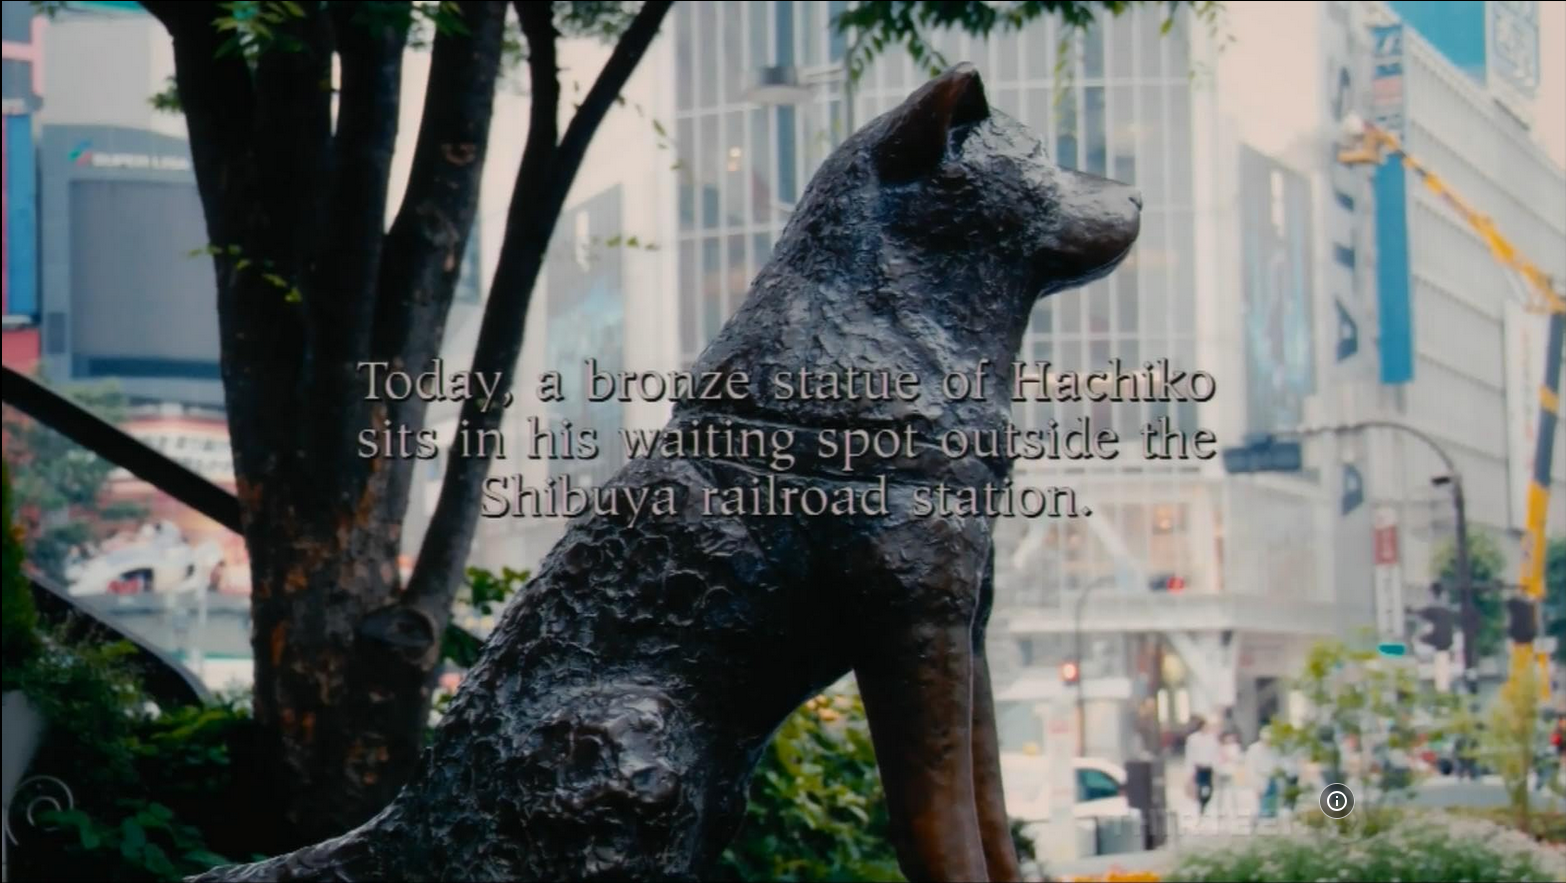
\includegraphics[width = 12cm]{Hachiko_statue}
	\caption{Hachiko dog's statue in Shibuya, Japan.}
\end{figure}
\begin{quotation}
	``The real {\sc Hachiko} was born in Odate Japan in 1923. When his master, Dr. {\sc Eisaburo Ueno}, a professor at {\it Tokyo University} died in May, 1925. {\sc Hachi} returned to the Shibuya train station the next day \& for the next 9 years to wait.'' -- \href{https://www.imdb.com/title/tt1028532/}{\it Hachi: A Dog's Tale} (2009).
\end{quotation}
Con người thì khác. Nhiều người lạ lắm. Có vài người bạn chỉ cần giúp họ 1 lần, họ sẽ nhớ ơn bạn cả đời \& cố gắng để trả ơn hết sức có thể, như nhân vật {\sf Hồng [agreeable giver]} \& {\sf Hồng [disagreeable giver]} trong tiểu thuyết ngắn này. Nhưng cũng có những kẻ chỉ cần bạn trót dại giúp họ 1 lần thôi, họ sẽ xem việc được bạn giúp là hiển nhiên, là nghĩa vụ của bạn. Họ sẽ đòi thêm, đòi nhiều hơn. Nếu bạn bớt giúp hoặc ngừng giúp thì họ sẽ hại \& tấn công bạn ngay, theo nghĩa vật lý hoặc tâm lý. Vết thương vật lý thì dễ lành, nhưng vết thương tâm lý, vết thương tinh thần có khi cả 1 đời vẫn không thể lành mà còn ngày càng tệ hơn. Giống như thí nghiệm tâm lý nổi tiếng trên các đứa trẻ trong 1 khu cô lập (mà thật ra yếu tố bị cô lập đối với xã hội hiện tại không còn cần thiết cho lắm): Nếu mỗi ngày bạn cho 1 đứa trẻ 1 số viên kẹo, đứa trẻ dần quen với việc được cho kẹo \& xem đó là trách nhiệm, là nghĩa vụ của bạn. Đến lúc bạn không còn cho nữa, đứa trẻ đó sẽ chửi bạn, thậm chí hãm hại bạn. Có nhiều người chưa trưởng thành, chưa làm yếu đi cái ác thuần túy của cái tính trẻ con ích kỷ, sẽ bóc lột, bắt nạt bạn cả đời chỉ vì 1 lần bạn lỡ dại giúp họ. Nguyên do là như thế: {\it the purest evil from the selfish \& childish soul -- cái ác thuần khiết nhất từ 1 tâm hồn trẻ con non nớt, ấu trĩ, \& ích kỷ}. Khi bạn chửi ai đó là `đồ chó' hay `con chó', hãy nhớ giúp tôi: {\it Đừng sỉ nhục \& làm vấy bẩn lòng trung thành của loài chó}.

Nếu bạn bắt nạt 1 chú chó, được ai đó hay chính bạn nuôi hoặc chó hoang, thì chúng tôi sẽ gọi ngay cho {\sf John Wick}\footnote{\href{https://www.imdb.com/title/tt2911666}{\it John Wick} (2014), \href{https://www.imdb.com/title/tt4425200}{\it John Wick: Chapter 2} (2017), \href{https://www.imdb.com/title/tt6146586}{\it John Wick: Chapter 3 -- Parabellum} (2019), \href{https://www.imdb.com/title/tt10366206}{\it John Wick: Chapter 4} (2023). Let's see when this film series ends, also {\it Fast \& Furious} series.} tới xử bạn: 1 lần \& mãi mãi. Mở rộng điều tương tự cho các động vật khác.

\subsubsection{On rat race -- Bàn về cuộc đua chuột}

``{\it``The Town Mouse \& the Country Mouse''} is 1 of \href{https://en.wikipedia.org/wiki/Aesop%27s_Fables}{Aesop's Fables}.'' -- \href{https://en.wikipedia.org/wiki/The_Town_Mouse_and_the_Country_Mouse}{Wikipedia{\tt/}The Town Mouse \& the Country Mouse}.

\begin{quotation}\it
	``The Country mouse gets used to live in safety, but doesn't get to eat delicious food like they have in the city. The Town mouse gets to eat delicious food, but runs a higher risk of being killed by humans or cats.'' -- {\sc Angel Devil}, \href{https://www.imdb.com/title/tt13616990/}{Chainsaw Man} (2022)
\end{quotation}
{\sf Tạm dịch}: Chuột quê đã quen với cuộc sống an toàn nhưng không được ăn những món ngon như ở thành phố. Chuột Thị trấn được ăn đồ ăn ngon nhưng có nguy cơ bị người hoặc mèo giết cao hơn.

Ta lấy chuột quê \& chuột thành phố để đua với nhau \& cá cược xem cá thể chuột của loại chuột nào sẽ thắng?

\begin{definition}[Rat race]
	``A \emph{rat race} is an endless, self-defeating, or pointless pursuit. The phrase equates humans to rats attempting to earn a reward such as cheese, in vain. It may also refer to a competitive struggle to get ahead financially or routinely. The term is commonly associated with an exhausting, repetitive lifestyle that leaves no time for relaxation or enjoyment.'' -- \href{https://en.wikipedia.org/wiki/Rat_race}{Wikipedia{\tt/}rat race}
\end{definition}
{\sf Tạm dịch}: Cuộc đua chuột là một cuộc theo đuổi vô tận, tự đánh bại hoặc vô nghĩa. Cụm từ này coi con người giống như những con chuột đang cố gắng kiếm phần thưởng như pho mát một cách vô ích. Nó cũng có thể đề cập đến một cuộc đấu tranh cạnh tranh để vượt lên về mặt tài chính hoặc thường xuyên. Thuật ngữ này thường gắn liền với một lối sống mệt mỏi, lặp đi lặp lại \& không có thời gian để thư giãn hay tận hưởng.

\begin{question}[On sacrificing people to entertain -- Bàn về việc hy sinh người khác để giải trí, tiêu khiển]
	Có nên để các loại chuột đua với nhau không? Có nên cá cược trên cuộc sống \& sinh mệnh của các cá thể khác không?
\end{question}

\begin{example}[P. Diddy \& The Aluminati?]
	Tại sao các ca sĩ nổi tiếng của Mỹ lại chết bởi tai nạn giao thông 1 cách trùng hợp vào ngày tế thần 25? Liệu có thế lực nào đó như Aluminati mà {\sc Jim Carrey} đã từng đề cập không ít lần, đứng sau thao túng tất cả? Rốt cuộc thì liệu cuộc sống của những người nổi tiếng (celebrities) chỉ là 1 sân khấu tiêu khiển, 1 đường đua chuột phiên bản con người của những kẻ quyền lực hiểm ác tàn độc thật sự, buôn bán cơ thể những người nổi tiếng như món hàng tình dục đắt tiền, rồi khi chơi chán thì sai khiến họ giết chóc nhau để tiếp tục tìm thú tiêu khiển ở 1 mức độ phê hơn, sướng hơn, i.e., tàn khốc hơn? Sởn gai óc khi mà điều này chợt khiến ta giật mình chợt nhớ lại câu trích dẫn của {\sc Kentaro Miura}: ``In this world, is the destiny of mankind controlled by some transcendental entity or law?'' or by real devils on Earth in the form of human beings like us? trong phần đầu tiểu thuyết này.
\end{example}
Đến đây thì cần đến sự xuất hiện của 1 nhân vật mới, thật ra là cũ, {\sf Trường [25; 1st-year mathematical PhD student in Austria]} -- 1 con chuột thành thị chính hiệu: a real town mouse. Kiểu học thức, sinh ra từ gia đình cha{\tt/}mẹ giáo viên, giỏi Toán \& nhiều môn khác, thủ khoa các kiểu, mọi thứ đều phải hoàn hảo tươm tất, chủ nghĩa cầu toàn? (perfectionism?), có sức hấp dẫn với những người thèm kiểu người đầy hiểu biết, nhưng chỉ tiếc là hắn sống với đầy định kiến về người khác. 1 con chuột phố như Trường không thể nào chấp nhận 1 con chuột quê như {\sf Hồng [25; 2nd-year mathematical PhD student in Germany]} có thể đi xa hơn hay leo cao hơn. Nếu Trường có 1 cái bảng đo thực lực của người khác hoặc cái kiếng đo chỉ số sức mạnh trong phim Dragon Balls (nên dịch ra là 7 Viên Ngọc Rồng chứ không phải bi rồng) thì ai mà vượt quá cái bảng chỉ số định kiến đó là sẽ có chuyện, e.g., tìm cách đạp các con chuột quê hôi hám, bẩn thỉu, hạ đẳng đó xuống, hoặc ít nhất là cút ra khỏi lãnh địa thiêng liêng của Toán học. Trường sẽ kiếm đến tận chỗ ở để ``giao lưu'', ``tìm hiểu'', săm soi khuyết điểm, \& quan trọng hơn là sẽ có những chiến thuật để thả những con rắn cái lai mèo độc hại như nhân vật {\sf Trinh [26{\tt/}27?; Amazon junior software developer; demanding taker, covert aggressive narcissist]} để cắn Hồng, làm Hồng phát suy \& trở nên yếu đi để dễ dàng thao túng \& kiểm soát. 1 định kiến sâu sắc mà những con chuột quê như {\sf Hồng [25; 2nd-year mathematical PhD student]} không bao giờ hiểu tại sao mình có cố gắng sống tốt \& làm bạn với chuột thành thị đều bất thành.

Trong khi Hồng có thể chơi đùa \& ăn uống thoải mái với các bạn người Brazil (nổi tiếng ăn cắp vặt), \& các bạn châu Phi (nổi tiếng ở bẩn \& mùi hôi tự nhiên của cơ thể) lúc còn ở Pháp, hay dân Maroc lúc còn ở Đức, thì ngược lại, Trường dứt khoát nói không với dân da đen. Sự cách biệt giữa chuột quê \& chuột phố sâu sắc tới mức thấm sâu vào từng ngóc ngách của thói quen, cách nhìn, cách sinh hoạt, cách chọn người để giao thiệp, nói chung là cách thức 1 cá thể tương tác 1 cách chọn lọc với 1 số người cũng như cách thức cá thể đó tham gia vào các hoạt động xã hội rộng lớn hơn.

Trường không bao giờ cho Trinh chơi với nhóm bạn riêng của Trường vì sợ Trinh làm dơ bất cứ ai trong cái nhóm đó, nhưng sẵn lòng thí Hồng cho Trinh. Đấy là mấu chốt về cái ``tình bạn'' mà Hồng luôn ảo tưởng, luôn mơ mộng về việc tìm 1 người cộng tác (a real collaborator \& a true friend) lâu dài trên con đường nghiên cứu Toán học. This is not Friendship. This is not Collaboration. This is Destruction. Nhưng Hồng có làm gì sai? Có lẽ việc bị (?) sinh ra từ 1 gia đình nông dân nghèo kiết xác là cái tội lỗi lớn nhất không thể cứu vãn mà hắn sẽ mang theo suốt cuộc đời này để chịu sự trù dập, sự dày vò, các thủ đoạn hãm hại không thương tiếc của những con người đầy định kiến tương tự. {\it Maybe poverty is a real sin in this scenario}.

Hồng thì lúc nào cũng giúp Trinh. Nhưng Trinh thì  coi việc được giúp như lẽ hiển nhiên. Kẻ yếu phải phục vụ kẻ mạnh, cho kẻ mạnh chà đạp lên. Trinh lúc nào cũng khinh Hồng. Trinh thèm chơi với Trường. Người giỏi chơi với người giỏi. Con giáo viên chỉ chơi với con giáo viên hoặc tầng lớp cao hơn hoặc ngang bằng: only $\ge$ or better $\gg$, not $<$ or worse $\ll$ ({\it Worse is Better?} Not a single chance!), không thèm chơi với con nông dân. Được lợi dụng là phúc phần rồi nên phải tự biết thân biết phận mà cảm thấy may mắn \& hạnh phúc. Gió tầng nào gặp mây tầng đó. Cũng 1 cái bảng định kiến tương tự sinh ra từ cái cuộc thi Học Sinh Giỏi Quốc Gia THPT như trong quyển \cite{Long2021}: {\it Học Trường Chuyên -- Những Góc Nhìn Đa Chiều} -- Bảng Phong Thần: chia tách súc sanh, thường dân, \& thánh nhân. Toàn dạng á khoa, thủ khoa. Hồng thì chả bao giờ ham mấy chuyện đó, nhưng hắn thừa biết là nước ngoài họ đòi hỏi ở mức độ rất khác mà thủ khoa Việt Nam chưa chắc ăn thua gì: Đấy là 1 mức độ ám ảnh về ham muốn am hiểu sâu sắc của tri thức. \& đây là nước Đức.

Hồng lại thêm 1 lần nữa thất vọng trong việc giúp đỡ người khác. Hắn vẫn chưa tởn. Nhìn cái mối quan hệ Trường--Trinh đầy phức tạp\footnote{Thêm nhân vật Trung ăn cắp sách nữa: Cái quái gì đang xảy ra với mấy đứa tên chữ `Tr' lứa sinh năm 1995--1996 thế hả {\sc Malcom Gladwell}?}, Hồng chợt nhớ tới chị Phương hồi ở Pháp. Hồng giúp Phương thì Phương thù, Phương ghét, Phương khinh, Phương đạp. Thọ hại Phương, thao túng tâm lý Phương thì Phương thờ, Phương phụng. Trinh cũng thế. Chả đâu vào đâu. Những cái định kiến mệt mỏi của cuộc đời khiến Hồng chả muốn tiếp tục làm người tốt. Nhưng cái lõi của Hồng là người tốt, hoặc ít nhất mẹ hắn nắn hắn thế. Thành ra Hồng mệt mỏi trong chuyện làm người, sống như 1 con người đúng nghĩa. Lòng tốt thì bị khinh. Còn bị, à nhầm, được thao túng tâm lý thì phê lắm, sướng lắm, như kiểu máu M, cứ sáp vô kẻ hãm hại hoặc kẻ thao túng như hiệu ứng Stockholm khi mà con tin bị bắt cóc dần yêu kẻ bắt cóc \& không thể tách rời được. Tâm lý con người quả là 1 mớ hỗ lốn đầy khó hiểu, muốn hiểu thì lại nhức đầu, rồi chả đâu vào đâu, ấy vậy mà 1 phần nhân cách của con chuột quê như Hồng lại quyết định trở thành nhà Tâm lý học rồi quyết tâm làm điều đó. Thế mới hài. {\it Just another serious joke in the $\infty$ series of jokes}. Just let me inherit a small piece of your huge legacy, {\sc David Foster Wallace}.

\subsubsection{On hatred vs. forgiveness -- Bàn về lòng căm hận vs. sự tha thứ}

\begin{quote}
	{\sf Hồng [28; psychologist \& phisopher]}: Khi cậu tiến lên 1 nền tảng về nhận thức cao hơn, cậu sẽ không còn căm hận các kẻ thù của cậu nữa. Không phải vì cậu tỏ vẻ thương hại họ để tự lừa dối bản thân, nhằm che đậy phức cảm tự ti (inferiority complex) 1 cách sợ hãi \& dữ dằn như 1 con mèo mẹ hoang xù lông lên khi cậu cố bắt con của nó, \& bợ đít cái phức cảm thượng đẳng (superiority complex) để tỏ ra 1 cách đầy giả tạo kiểu cậu đã trở thành dạng thánh thần, đã đạt tới cảnh giới Niết bàn trong Phật giáo. Đơn giản là khi cậu tiến lên 1 nền tảng về nhận thức cao hơn, cậu sẽ thấu hiểu vì sao các kẻ thù của cậu lại làm thế với cậu, tại sao họ hại cậu \& giúp cậu tự hại cậu, cậu hiểu nguyên nhân về tâm lý của từng đối tượng ấy 1 khi cậu đã rành đường trong địa hạt Tâm Lý Học (Psychology $\Psi$), rồi cậu hiểu nguyên nhân sâu xa hơn về mặt xã hội 1 khi cậu rành đường hơn trong địa hạt Xã Hội Học (Sociology), cậu sẽ bắt đầu tha thứ cho họ, để có thể tha thứ cho bản thân cậu. Thay vì cảm thấy hận thù, cậu thấy tội nghiệp cho họ, hệt như cái cách mà {\sf Itadori Yuji} tội nghiệp nguyền hồn {\sc Ryomen Sukuna} trong {\it Jujutsu Kaisen -- Chú Thuật Hồi Chiến} trước khi hủy diệt hắn vậy. This is the Ultimate Empathy -- lòng thấu cảm tột cùng. Tiến lên 1 nền tảng cao hơn đơn giản là việc cậu rành đường ở nhiều địa hạt quan trọng khác nhau thay vì cứ lạc lối trong tâm trí \& linh hồn của cậu. Tới đây cậu đã bớt lạc đường hơn, không còn sợ bị bỏ rơi nữa thì cũng có lẽ là lúc cậu phải tự bước đi trên đôi chân của mình \& gánh vác các tránh nhiệm cần thiết trên đôi vai của cậu, dẫu chúng có nhỏ bé \& yếu ớt tới mức nào đi chăng nữa. You have to go there to see it, to feel it, \& then to live with it, the Tree of Life in {\it Attack on Titan}. But in order to go there, you have to live, to work, to think, to reflect yourself, to balance between living \& working, to feel the flow of this life, all the pains inside it, also all the loves inside it. You must practice day by day. You will get there at the end of your life in this physical world $\mathbb{R}^3$, before transferring to another realms of the soul if there is any.
\end{quote}

\subsection{The last moonwalk in the Inferno -- Điệu nhảy moonwalk cuối cùng ở Hỏa Ngục}

\paragraph*{Dark triad -- Bộ 3 đen tối.} Những kẻ ái kỷ cần học cách quan tâm, yêu thương người khác cho dù họ không có bất cứ cảm giác chân thành nào. Những kẻ xảo quyệt cần bớt gian xảo \& học cách cư xử thành thật hơn. Những kẻ chống đối xã hội nên tập chung tay xây dựng cộng đồng, dù chỉ là đạo đức giả, nhưng quan trọng là hành động. Những kẻ thái nhân cách nên bớt hãm hại người khác 1 cách tàn độc. 3 ba đen tối nên học cách giúp đỡ, thấu hiểu người khác, tập cảm nhận niềm tin, lòng chân thành, sự thấu cảm để cải thiện nhân cách \& các thiếu sót về mặt cấu trúc, chức năng của não bộ theo khía cạnh Khoa học Thần kinh để hòa nhập với cộng đồng theo xu hướng tích cực cho cả bản thân \& cho cộng đồng mà họ có ảnh hưởng tới.

\paragraph*{Teacher-student relationship -- tình sư trò.} I will continue your legacies (i.e., inherit, develop, \& upgrade like a developer), all of my teachers, \& then I will find someone to continue mine. So, now I need to built my legacy. I am building it. Someone will inherit it someday. \& his{\tt/}her students will inherit his{\tt/}hers. Life goes on \& on. Goodness \& positivity need spreading on this Earth, in human communities in particular \& in the whole human society in general, \& in the animal kingdoms, through realms of Psychology $\Psi$, Philosophy $\Phi$, \& Spirituality.

Tôi sẽ tiếp tục các di sản của tất cả thầy cô của tôi, i.e., tôi sẽ kế thừa, phát triển, \& nâng cấp chúng lên, \& rồi tôi sẽ tìm ai đó để kế thừa các di sản của tôi (các học trò của tôi). Cho nên bây giờ tôi nên bắt đầu xây dựng di sản của mình. Tôi đang làm điều đó. Ai đó rồi sẽ kế thừa nó vào 1 ngày nào đó. \& các học sinh, sinh viên của (những) người đó sẽ tiếp tục kế thừa các di sản của người đó. Cuộc sống cứ thế tiếp diễn. Các điều tốt lành \& tích cực cần được lan truyền rộng rãi trên Trái Đất này, trong các cộng đồng loài người nói riêng \& tổng thể xã hội loài người nói chung, \& trong các vương quốc của loài vật, xuyên qua các địa hạt của Tâm Lý Học $\Psi$, Triết Học $\Phi$, \& Tâm Linh Học.

%------------------------------------------------------------------------------%

\section{Miscellaneous -- Linh tinh}

%------------------------------------------------------------------------------%

\appendix

%------------------------------------------------------------------------------%

\section{Acknowledgment -- Lời tri ân}
We, the authors, apologize to save this part for the last. Set the {\it acknowledgment switch variable} is $\delta_{\rm ack}$. Đặt {\it biến công tắc cảm ơn} là $\delta_{\rm ack}$\footnote{Distinguished with {\sc Mikasa Ackerman} or {\sc Levi Ackerman} in {\it Attack on Titan}.}.

\begin{Verbatim}[numbers=left,xleftmargin=5mm]
if project_evaluation = fail
    take_all_responsibility = enabled;
else {
    take_all_credit = disabled;
    distribute_credit;
    acknowledgment;
}
\end{Verbatim}
We thank all the people who helped us, have helping us, also who, without knowing it, made me what I am today \& made us what we are today.

Xin cảm ơn các bài viết sâu sắc về giáo dục của thầy{\tt/}Dr. {\sc Trần Nam Dũng}, về giáo dục \& nghiên cứu Toán cao cấp của thầy{\tt/}Prof. {\sc Nguyễn Hữu Việt Hưng}, Prof. {\sc Ngô Bảo Châu}, Prof. {\sc Hà Huy Khoái}, Prof. {\sc Phan Thành Nam}, Prof. {\sc Đào Hải Long}. 2 tác giả không hề có bất cứ trao đổi nào với các người thầy này, nhưng bài viết của họ đã đủ để các tác giả bắt tay vào chấp bút cho 1 số ý tưởng của phần bàn về việc học \& bàn về việc dạy. Nếu có bất cứ lỗi nào xảy ra trong tiểu thuyết, đó hoàn toàn là lỗi của 2 tác giả đã hiểu sai ý từ các bài viết gốc. Hoàn toàn không liên quan đến ý tốt hay các tư tưởng của những người thầy này.

Xin chân thành những người đã từng giúp, đã từng thương hoặc thương hắn đến tận ngày hôm nay. Cuộc hành trình mưu cầu hạnh phúc \& khám phá tri thức sẽ thật khó khăn nếu không có họ củng cố niềm tin của 2 tác giả. Xin cảm ơn chị{\tt/}Dr. {\sc Lê Thị Minh Thảo}, anh {\sc Hoàng Công Đức}, anh{\tt/}thầy{\tt/}Dr. {\sc Lê Phúc Lữ}, anh{\tt/}thầy{\tt/}Dr.  {\sc Đào Mạnh Khang}, chị{\tt/}Dr.  {\sc Lan Hương}, anh{\tt/}thầy{\tt/}Dr.  {\sc Đào Nguyên Anh}, Prof. {\sc Jesús Ildefonso Díaz}, thầy{\tt/}anh{\tt/}Dr.  {\sc Trà Quốc Khanh}, thầy{\tt/}anh {\sc Lê Văn Chánh}, cô {\sc Lê Thị Thanh Lĩu}, cô {\sc Dương Thị Xuân An} đã truyền động lực trên hành trình học Toán của 2 tác giả. Xin cảm ơn cô {\sc Đặng Thị Hạnh}, cô {\sc Đặng Thị Bích Thư}, thầy {\sc Võ Văn Huynh} đã viếng đám tang của cha 2 tác giả, để họ không bị nỗi sợ bị bỏ rơi nuốt chửng. Xin cảm ơn thầy {\sc Lê Hoàng Minh}, thầy {\sc Nguyễn Thanh Tài}, thầy {\sc Võ Văn Huynh}, thầy {\sc Đệ}, thầy {\sc Lê Thanh Hải}, thầy {\sc Trần Thanh Liêm}, thầy {\sc Nguyễn Văn Quí}\footnote{Rest In Peace, my respected Elementary Mathematics teacher. I dedicate this work \& future works on Mathematics, both Elementary \& Advanced, \& their bridges, connections, for you.}, thầy{\tt/}Dr.  {\sc Trần Nam Dũng}, thầy{\tt/}Dr. {\sc Nguyễn Tấn Trung}, thầy{\tt/}Prof. {\sc Huỳnh Quang Vũ}, thầy{\tt/}Prof. {\sc Đặng Đức Trọng}, đã là những mẫu hình người thầy tuyệt vời để 2 tác giả bắt chước theo. Phải trưởng thành mà không có sự giúp đỡ \& hình mẫu của người cha (father as a role model) trong điều kiện thiếu thốn cả về kiến thức, vật chất, lẫn tinh thần, thật không dễ dàng gì.

We apologize that we should start this project sooner. But the struggle to mentally grow up is great \& devastating enough to prevent us from doing that.

Bạn đọc có thể dễ dàng nhận thấy đây là 1 chủ đề vô cùng nhạy cảm, cực kỳ nguy hiểm. Nên nếu dự án này thất bại, thì đều do sự non nớt của 2 tác giả với ngòi bút chưa đủ sắc bén nên không thể giải phẫu vấn đề này đến nơi đến chốn, không liên quan gì đến bất cứ ai \& khẳng định là không ai giúp 2 tác giả trong tiểu thuyết này. 2 tác giả xin hoàn toàn chịu trách nhiệm về sự thất bại nếu có.

%------------------------------------------------------------------------------%

\section{Lists -- Các Danh Sách}
We, the authors, love making \st{love} lists. Chúng tôi, 2 tác giả, thích tạo ra các danh sách.

\subsection{A summary list of goals -- Danh sách tổng hợp các mục tiêu}

\begin{goal}[Mental maps -- các tấm bản đồ tinh thần]
	Quyển sách này là 1 quyển sách nhỏ nói về các quyển sách mà 2 tác giả cho là cần thiết đối với học sinh cấp 2 bắt đầu tuổi dạy thì, học sinh cấp 3 chuẩn bị bước vào trường Đại học hoặc trường đời hoặc cả 2, cho các sinh viên mới ra trường bắt đầu hoang mang kiếm việc làm, cũng như 1 tài liệu tham khảo dành cho quý phụ huynh, quý thầy cô, những người quan tâm đến giáo dục con cái, trẻ em, học sinh, sinh viên của mình. Quyển sách đóng vai trò như 1 cái Google Map, nhưng không phải về Địa Lý trong thế giới Vật Lý, mà trong thế giới của Tâm Trí để giúp các bạn trẻ không bị lạc đường, đặc biệt là các bạn thiếu sự quan tâm, tình thương của cha mẹ, \& các bạn mất cha hoặc mẹ hoặc cả 2. Quyển sách cũng nhằm mục đích cho các bạn học sinh, sinh viên, nghiên cứu viên có 1 cái nhìn thực tế để mường tượng ra được rìa bên kia thế giới, ý là du học, chứ không phải siêu thoát.
\end{goal}

\begin{goal}[Acknowledgment -- tri ân]
	Quyển sách là 1 lời tri ân đối với các người anh, người chị, thầy cô, những người đã từng giúp 2 tác giả. 2 tác giả nghĩ rằng việc viết 1 chuỗi các quyển sách là cách trả ơn giáo dục thiết thực nhất.
\end{goal}

\subsection{A summary list of principles -- Danh sách tổng hợp các nguyên lý}

\begin{principle}[Principle of positivity non-conservation -- Nguyên lý về sự không bảo toàn của tính tích cực]
	If there is a huge loss of psychological positivity that a person has tried to generate \& spread to other people around that person, then there exists at least a psychological manipulator in the role of the psychological Black Hole with the purpose of destroying all the positivities \& generating negativities \& then spread to people surrounding that psychological manipulated victim.
\end{principle}

\subsection{A summary list of rules -- Danh sách tổng hợp các nguyên tắc}

\begin{enumerate}
	\item {\it On judgment -- Bàn về phán xét.} Không phán xét, công kích, e.g., dí trên mạng xã hội, bất cứ ai. Cũng không áp đặt ai, thậm chí cả việc áp đặt ai đó không được áp đặt người khác. Tạo cho người khác 1 cảm giác thoải mái tối thiểu khi tiếp xúc.
	\item {\it On stalking -- Bàn về rình rập.} Không quá tò mò vào cuộc sống cá nhân của người khác, e.g., stalk in social media -- rình mò trên các nền tảng mạng xã hội, xâm phạm tài khoản  riêng tư cá nhân bất hợp pháp. Keep healthy boundaries for both.
	\item {\it On system reset -- Bàn về khởi động lại hệ thống.} Một phản tư xa hơn trong tương lai có lẽ là chẳng có hành trình phát triển tự thân nào mà đủ sức chống chọi 1 cách hiệu quả với các tương tác xã hội cả, đặc biệt là các tương tác xấu \& các mối quan hệ độc hại (toxic relationships) cả. Khi đó thì tất cả các ghi chú ở đây sẽ bị xóa. Mọi thứ trở về cấu hình sống nhiều mặt phổ dụng để che giấu bản thân.	
	\item {\it On humanity development -- Bàn về phát triển nhân cách.} Dẫu cho bạn làm bất cứ ngành nghề nào, đừng quên nhiệm vụ chính của việc làm người là phát triển nhân cách 1 cách toàn diện. Đừng phát triển nhân cách theo xu hướng của 1 kẻ khốn nạn, thích bắt nạt bất cứ ai mà bạn cho là dưới cơ hay yếu thế hơn bạn.
	\item {\it On reading Wikipedia -- Bàn về chăm đọc Wikipedia.} Dạy học sinh bắt đầu tìm hiểu mọi thứ bằng Google \& chăm đọc Wikipedia tiếng anh nhiều vào, để xem có thể hiểu đến đâu.
	\item {\it On bullying -- Bàn về việc bắt nạt.} Trước khi bạn quyết định bắt nạt hoặc hãm hại 1 ai đó, tự hỏi bản thân là nếu thay đổi vị trí cho nhau thì bạn có thích bị bắt nạt hay hãm hại như thế không. Hoặc hơn thế, liệu con bạn trong tương lai có thể chịu những hành vi mà bạn đang áp lên người khác, liệu bạn có chịu nổi những gì tương tự sẽ xảy ra với con cái của bạn không?
	\item {\it On stupidity -- Bàn về sự ngu dốt.} Take responsibility of your stupidity. Do not let your stupidity, no matter if you are aware of it or not, harm or even destroy any person in the aspect of either his{\tt/}her (private) personal life or professional career or both.
	
	-- Chịu trách nhiệm cho sự ngu dốt của bạn. Đừng để sự ngu dốt của bạn, dù bạn có nhận thức được nó hay không đi nữa, làm hại hoặc hủy hoại bất cứ ai trong khía cạnh cuộc sống cá nhân (riêng tư) \&{\tt/}hoặc sự nghiệp của người đó.
	\item {\it On deserving responsibility -- Bàn về sự xứng đáng về trách nhiệm.} Only take responsibility for whom deserved your responsibility. -- Chỉ chịu trách nhiệm cho ai xứng đáng với trách nhiệm của bạn.
\end{enumerate}

\subsection{A summary list of $\Psi$-theorems, $\Phi$-theorems -- Danh sách tổng hợp các ``định lý'' về tâm lý \& triết học}

\begin{psy-theorem}[Eidetic memory $+$ critical thinking $+$ integrity vs. $\Psi$-manipulation]
	A combination of eidetic memory, a sharp critical thinking, \& a high enough integrity is a natural enemy of psychological manipulation. Consequently, eidetiker with a sharp critical thinking \& a high enough integrity is a natural enemy of psychological manipulators.
	
	-- 1 tổ hợp của trí nhớ điện tử, 1 tư duy phản biện sắc bén, cùng 1 sự chính trực đủ cao là 1 trong những thiên địch của thao túng tâm lý. Hệ quả là kẻ có trí nhớ điện tử với 1 tư duy phản biện sắc bén cùng 1 lòng chính trực đủ cao là 1 trong những thiên địch của các kẻ thao túng tâm lý \& các kẻ tiểu nhân.
\end{psy-theorem}

\begin{psy-theorem}[Art of balancing in life]
	Cố gắng cho đi những người cần sự giúp đỡ của bạn \& xứng đáng với nó, cùng sự phòng thủ đối với các nhân cách độc hại, e.g., các kẻ thao túng tâm lý, bộ 3 đen tối (kẻ ái kỷ, kẻ chống đối xã hội, kẻ thái nhân cách), cố gắng học từ các nỗi đau trong quá khứ \& hiện tại, chấp nhận các nỗi đau sẽ tới trong tương lai, đi thăng bằng trên chiếc xe đạp của {\sc Albert Einstein}, với thanh thăng bằng có 1 bên là đạo đức, 1 bên là lương tâm, cố gắng tối ưu hóa việc tạo ra sự tích cực của cá nhân cho cuộc sống của cộng đồng mà bạn có ảnh hưởng tích cực tới.
\end{psy-theorem}

\section{Authors Bibliography -- Đôi điều về các tác giả}

\begin{enumerate}
	\item {\sc Nguyễn Quản Bá Hồng} (1996--?): Tự thân vận động để đậu lớp chuyên Toán khóa 2011--2014 dưới sự ngăn cấm thi trường chuyên của cha mẹ do hoàn cảnh nghèo rớt mồng $\ldots$, à nhầm, không có cọng mồng tơi để rớt của gia đình. Kẻ hủy diệt ngôn ngữ (Vietnamese Literary Destroyer) khiến gần như tất cả các giáo viên dạy Văn của trường chuyên đều ghét, hoặc ít nhất là không ưa. Kẻ dốt tiếng Anh (English Destroyer) nên được học bổng du học mà chưa có bằng {\sc Ielts} hay {\sc Toefl}. May mắn được phép học Thạc sĩ năm cuối, bỏ Thạc sĩ năm đầu (straight into Master 2, skipped Master 1) ở Đại học Rennes 1 (University of Rennes 1\footnote{Universit\'e de Rennes 1: \url{https://www.univ-rennes.fr/}.}, France) trong lớp ENS của Rennes \& ENS Paris trộn lại. Tiến sĩ Toán Tối Ưu {\it hụt} tại Đại học Humboldt ở Berlin, Đức (Humboldt University of Berlin\footnote{Humboldt-Universität zu Berlin: \url{https://www.hu-berlin.de/en}.}) khi còn làm việc ở Viện Weierstrass (Weierstrass Institute for Applied Analysis \& Stochastics\footnote{Weierstraß-Institut für Angewandte Analysis und Stochastik: \url{https://www.wias-berlin.de/}.}) với sự hỗ trợ của quỹ Marie--Curie -- 1 trong những quỹ khoa học danh giá bậc nhất châu {\sc âu}.
	
	Yêu chó [Dog\st{(gy)} Lover]. Yêu \st{sex} sách (Book Lover). Yêu sự chân thành, ghét sự giả dối. Sẵn sàng \st{từ bỏ xu hướng tính dục \& dục vọng} dùng vài năm không bon chen kiếm việc lương cao, sẵn sàng thí nghiệm tâm lý lên chính bản thân để đạt được mục tiêu riêng nhưng có thể có ích chung, nhốt mình ở nhà để viết 1 cuốn \st{tự truyện (autobiography)} tiểu thuyết hư cấu ngắn (a short fictional novel) để khóa mõm các kẻ thích bắt nạt trí tuệ \& nghiên cứu về các nhân cách độc hại, có tác động xấu đến người khác \& các cộng đồng.
	
	Hắn là kiểu sinh ra trong gia cảnh nghèo mà có tính cầu toàn khó ưa. Eo ơi cái chủ nghĩa hoàn hảo (perfectionism) chết tiệt! Hắn có thể phá hủy cả 1 tác phẩm do hắn làm (hắn tôn trọng bất cứ tác phẩm nào của người khác nên không có chuyện hắn phá tác phẩm của người khác) chỉ đơn giản vì hắn không thích 1 (vài) chi tiết nào trong tác phẩm đó mà hắn không thể sửa được. Điểm này giống nhân vật {\sc Rust Cohl} trong series film \href{https://www.imdb.com/title/tt2356777/}{True Detective}:
	\begin{quotation}\it
		``Rust would pick a fight with the sky if he didn't like its shade of blue. But when we finally got him over to the house - this is when that case was hot - the bastard looks like he was on his way to firing squad.'' -- \href{https://www.imdb.com/title/tt2356777/}{True Detective} (2014--) [S1.E1].
	\end{quotation}
	\begin{itemize}
		\item CV: {\sc url}: \url{https://github.com/NQBH/publication/blob/master/CV/NQBH_CV.pdf}.
		\item Website: {\sc url}: \url{https://nqbh.github.io}.
		\item Trang web của {\it Some Topics in Elementary STEM \& Beyond -- Vài Chủ Đề Trong STEM Sơ Cấp \& Hơn Thế Nữa}: {\sc url}: \url{https://nqbh.github.io/elementary_STEM}.
		\item Trang web của {\it Some Topics in Advanced STEM \& Beyond -- Vài Chủ Đề Trong STEM Cao Cấp \& Hơn Thế Nữa}: {\sc url}: \url{https://nqbh.github.io/advanced_STEM}.
		\item E-book library -- Thư viện sách điện tử: {\sc url}: \url{https://github.com/NQBH/reference}.
		\item File bibliography {\tt bib.bib} dùng để quản lý danh mục sách điện tử: {\sc url}: \url{https://github.com/NQBH/reference/blob/master/bib.bib}.
	\end{itemize}
	
	\item {\sc Nguyễn Quản Trung Nhân} (?--?): Classified information -- thông tin tuyệt mật. You can read some from this book, but there is no information given further.
\end{enumerate}

\subsection{Versions -- Các phiên bản}
Bạn đọc có thể truy cập lịch sử cập nhật, cùng các phiên bản trước đó nếu có 1 sự hiểu biết tối thiểu về công cụ quản lý phiên bản Git hoặc chịu khó mò mẫm đủ lâu.
\begin{itemize}
	\item The last updated version of this short novel is stored at the following (permanent?\footnote{This permanence depends on the fact that stalkers such as {\sf Trung [21], Trinh [27]}, \& {\sf Axel Kr\"oner [$\approx$ 45--50]} in this short novel still like to invade personal \& private account to see all secrets of someone, e.g., the authors of this fictional novel, \& then decide to delete some files or destroy all repositories again.}) link:\\{\sc url}: {\sf\small\url{https://github.com/NQBH/elementary_STEM_beyond/blob/main/learning_teaching_research/NQBH_on_learning_teaching_research.pdf}}.
	
	Bản cập nhật mới nhất của tiểu thuyết này được lưu trữ ở đường dẫn (cố định?\footnote{Việc cố định còn phụ thuộc vào những kẻ rình rập (stalkers) như 3 nhân vật {\sf Trung [21], Trinh [27]}, \& {\sf Axel Kr\"oner [$\approx$ 45--50]} trong tiểu thuyết vẫn còn thích thâm nhập vào tài khoản cá nhân của người khác để lục tung lên rồi có quyết định xóa thành quả lao động của người khác nữa hay không.}):\\{\sc url}: {\sf\small\url{https://github.com/NQBH/elementary_STEM_beyond/blob/main/learning_teaching_research/NQBH_on_learning_teaching_research.pdf}}.
	\item {\it Some Thoughts On Learning, Teaching, \& Research: A Short Novel -- Vài Suy Nghĩ Về Việc Học, Việc Dạy, \& Nghề Nghiên Cứu: 1 Tiểu Thuyết Ngắn: Comments \& Donations -- Bình Luận Góp Ý \& Quyên Góp}.
	
	Folder: {\sf Elementary STEM \& Beyond{\tt/}learning, teaching, \& research{\tt/}comments \& donations}: [\href{https://github.com/NQBH/elementary_STEM_beyond/blob/main/learning_teaching_research/comment_donation/NQBH_learning_teaching_research_comment_donation.pdf}{pdf}\footnote{{\sc url}: \url{https://github.com/NQBH/elementary_STEM_beyond/blob/main/learning_teaching_research/comment_donation/NQBH_learning_teaching_research_comment_donation.pdf}.}][\href{https://github.com/NQBH/elementary_STEM_beyond/blob/main/learning_teaching_research/comment_donation/NQBH_learning_teaching_research_comment_donation.tex}{\TeX}\footnote{{\sc url}: \url{https://github.com/NQBH/elementary_STEM_beyond/blob/main/learning_teaching_research/comment_donation/NQBH_learning_teaching_research_comment_donation.tex}.}].
\end{itemize}
Tiểu thuyết này có 3 phiên bản với 3 cỡ chữ (font size) khác nhau:
\begin{itemize}
	\item 10pt ***link*** Dành cho người trẻ tuổi mắt tốt \& thích tiết kiệm giấy in.
	\item 11pt ***link*** 
	\item 12pt ***link*** dành cho người cao tuổi mắt kém.
\end{itemize}

\subsection{Price -- Giá bán}
Tiểu thuyết này cùng các tài liệu liên quan được bán với giá $x$ VND{\tt/}\${\tt/}\texteuro, với $x\in[0,\infty)$ là 1 số thực không âm, i.e., muốn trả bao nhiêu cũng được, tùy vào đánh giá độ hay, độ hữu ích theo nhu cầu, nhận thức, \& thị hiếu của bạn đọc.

{\it Lý do}: Nếu $x < 0$ thì bỏ 1 đống công sức ra phá sản thì không được thông minh cho lắm, không xứng đáng để dạy Toán \& đầu tư kinh doanh cho các lứa học sinh, sinh viên trong tương lai. Nên các tác giả từ chối bán với giá là 1 số thực âm. Còn nếu $x\in\mathbb{C}\backslash\mathbb{R}$, tức 1 số tiền ảo không thuần thực, i.e., $x = a + bi$ với $a\in\mathbb{R},b\in\mathbb{R}^\star$ thì phải xem lại `đồng tiền ảo' như Bitcoin, hay tệ hơn là Luna Coin xài được hay lâu dài hay không.

\subsection{Donation{\tt/}Payment -- Quyên góp{\tt/}Thanh toán}
\noindent\textbf{\textsf{Bank Transfer Information -- Thông tin chuyển khoản}}:
\begin{itemize}
	\item {\it Account Holder -- Chủ Tài Khoản}: {\sc Nguyễn Quản Bá Hồng}.
	\item {\it Bank -- Ngân hàng}: Ngân Hàng Thương Mại Á Châu{\tt/}Asia Commercial Bank (ACB).
	\item {\it Account Number -- Số Tài Khoản}: 1510717.
	\item {\it Branch -- Chi Nhánh}: ACB-CN Bến Tre.
\end{itemize}

%------------------------------------------------------------------------------%

\printbibliography[heading=bibintoc]
\label{ref}
	
\end{document}